\documentclass{article}
\usepackage[utf8]{inputenc}
\usepackage[T1]{fontenc}
\usepackage{amsmath}
\usepackage{amsthm}
\usepackage{bytefield}
\usepackage{graphicx}
\usepackage{newtxmath}
\usepackage{mathtools}
\usepackage{xspace}
\usepackage{url}
\usepackage{changepage}
\usepackage{enumitem}
\usepackage{tabularx}
\usepackage{hhline}
\usepackage[usestackEOL]{stackengine}
\usepackage{comment}
\usepackage{needspace}
\usepackage[nobottomtitles]{titlesec}
\usepackage[hang]{footmisc}
\usepackage{xstring}
\usepackage[usenames,dvipsnames]{xcolor}
\usepackage[unicode,bookmarksnumbered,bookmarksopen,allbordercolors=MidnightBlue,
            citebordercolor=Plum,urlbordercolor=BrickRed]{hyperref}
\usepackage{cleveref}
\usepackage{nameref}
\usepackage{etoolbox}
\usepackage{subdepth}
\usepackage{fix-cm}
\usepackage{hyphenat}
\usepackage{tocloft}

\usepackage[style=alphabetic,maxbibnames=99,dateabbrev=false,urldate=iso8601,
            backref=true,backrefstyle=none,backend=biber]{biblatex}
\addbibresource{zcash.bib}

% Fonts
\usepackage{lmodern}
\usepackage{quattrocento}
\usepackage[bb=ams]{mathalfa}
\usepackage[scr]{rsfso}
%\usepackage{txfonts}

% Quattrocento is beautiful but doesn't have an italic face. So we scale
% New Century Schoolbook italic to fit in with slanted Quattrocento and
% match its x height.
% (This has the side effect of making all italic text into boxes, so
% it won't linebreak, which has pluses and minuses.)
\renewcommand{\emph}[1]{\hspace{0.15em}{\fontfamily{pnc}\selectfont\scalebox{1.02}[0.999]{\textit{#1}}}\hspace{0.02em}}

% While we're at it, let's match the tt x height to Quattrocento as well,
% and compress it a little to save space in tables.
\let\oldtexttt\texttt
\let\oldmathtt\mathtt
\renewcommand{\texttt}[1]{\scalebox{0.97}[1.07]{\oldtexttt{#1}}}
\renewcommand{\mathtt}[1]{\scalebox{0.97}[1.07]{$\oldmathtt{#1}$}}

% bold but not extended
\newcommand{\textbnx}[1]{{\fontseries{b}\selectfont #1}}


\crefformat{footnote}{#2\footnotemark[#1]#3}

\DeclareLabelalphaTemplate{
  \labelelement{\field{citekey}}
}

\DefineBibliographyStrings{english}{
  page  = {page},
  pages = {pages},
  backrefpage = {\mbox{$\uparrow$ p\!}},
  backrefpages = {\mbox{$\uparrow$ p\!}}
}

\setlength{\oddsidemargin}{-0.25in}
\setlength{\textwidth}{7in}
\setlength{\topmargin}{-0.75in}
\setlength{\textheight}{9.2in}
\setlength{\parindent}{0ex}

\newcommand{\defaultarraystretch}{1.4}
\renewcommand{\arraystretch}{\defaultarraystretch}

% <https://tex.stackexchange.com/a/49898/78411>
\makeatletter
\renewcommand{\@pnumwidth}{2em}
\makeatother

\newcommand{\pagenumfont}{\fontfamily{pnc}\selectfont\rule[-.2\baselineskip]{0pt}{1.35\baselineskip}}
\renewcommand{\cftsecpagefont}{\pagenumfont}
\renewcommand{\cftsubsecpagefont}{\pagenumfont}
\renewcommand{\cftsubsubsecpagefont}{\pagenumfont}
\renewcommand{\cftparapagefont}{\pagenumfont}

\hfuzz=1pt
\overfullrule=2cm

\setlength{\footnotemargin}{0.6em}
\setlength{\footnotesep}{2ex}
\addtolength{\skip\footins}{3ex}

\renewcommand{\bottomtitlespace}{8ex}

% Use rubber lengths between paragraphs to improve default pagination.
% <https://tex.stackexchange.com/questions/17178/vertical-spacing-pagination-and-ideal-results>
\setlength{\parskip}{1.5ex plus 2pt minus 2pt}

\widowpenalties 3 10000 1000 0

\setlength{\bibitemsep}{1.2ex}  % default is too cramped!
\setlength{\biblabelsep}{0.5em} % default is not cramped enough! :-)

\setlist[enumerate]{before=\vspace{-0.8ex}}
\setlist[itemize]{itemsep=0.3ex,topsep=0.2ex,before=\vspace{-0.8ex},after=\vspace{1.5ex}}

\newlist{compactitemize}{itemize}{3}
\setlist[compactitemize]{itemsep=-1ex,topsep=0ex,before=\vspace{-0.2ex},leftmargin=1.2em,label=$\cdot$,after=\vspace{-3.3ex}}

\newlist{formulae}{itemize}{3}
\setlist[formulae]{itemsep=0.2ex,topsep=0ex,leftmargin=1.5em,label=,after=\vspace{1.5ex}}

\newlist{lines}{itemize}{3}
\setlist[lines]{itemsep=-0.5ex,topsep=0ex,before=\vspace{1ex},leftmargin=1.6em,label=,after=\vspace{1ex}}


\makeatletter
\renewcommand*{\@fnsymbol}[1]{\ensuremath{\ifcase#1\or \dagger\or \ddagger\or \mathsection\or \mathparagraph\else\@ctrerr\fi}}
\makeatother

\newcommand{\slightlylarge}{\fontsize{10.5}{10.5}\selectfont}
\newcommand{\notsolarge}{\fontsize{11}{11}\selectfont}
\newcommand{\largeish}{\fontsize{12}{12}\selectfont}
\newcommand{\larger}{\fontsize{13}{13}\selectfont}
\newcommand{\Larger}{\fontsize{16}{16}\selectfont}

\titleformat*{\subsection}{\larger\bfseries}
\titleformat*{\subsubsection}{\largeish\bfseries}
\titleformat*{\paragraph}{\notsolarge\bfseries}
\titleformat*{\subparagraph}{\slightlylarge\bfseries}

% Fix the height of citation link underlines.
% Also, biblatex really doesn't want to support Unicode citation labels, but I will not be beaten.
\newcommand{\linkstrut}{\rule[-0.4ex]{0ex}{\fontcharht\font`X}}
\DeclareFieldFormat{labelalpha}{\linkstrut\smash{\StrSubstitute{#1}{MAEA2010}{MAEÁ2010}}}
\DeclareFieldFormat{postnote}{\linkstrut\smash{#1}}
\let\oldcite\cite
\renewcommand{\cite}[2][]{\raisebox{0ex}{\oldcite[{#1}]{#2}}}

\let\oldfootnote\footnote
\renewcommand{\footnote}[1]{\hairspace{\oldfootnote{#1}}}
\newcommand{\footnotewithlabel}[2]{\hairspace\oldfootnote{\label{#1}{#2}}}

\newcommand{\crossref}[1]{\raisebox{0ex}{\autoref{#1}}\hspace{0.2em}\emph{`\nameref*{#1}\kern -0.05em'} on p.\,\pageref*{#1}}
\newcommand{\theoremref}[1]{\raisebox{0ex}{\autoref{#1}} on p.\,\pageref*{#1}}
\newcommand{\footnoteref}[1]{\hairspace\raisebox{0ex}{\cref{#1}}}

\newcommand{\autorefprefix}{\linkstrut\S\!}
\renewcommand{\sectionautorefname}{\autorefprefix}
\renewcommand{\subsectionautorefname}{\autorefprefix}
\renewcommand{\subsubsectionautorefname}{\autorefprefix}
\renewcommand{\paragraphautorefname}{\autorefprefix}
\renewcommand{\subparagraphautorefname}{\autorefprefix}

%\let\oldhref\href
%\renewcommand{\href}[2]{\raisebox{0ex}{\oldhref{#1}{\linkstrut\smash{#2}}}}
%\let\oldurl\url
%\renewcommand{\url}[1]{\href{#1}{\nolinkurl{#1}}}

% <https://tex.stackexchange.com/a/60212/78411>
\newcommand{\subsubsubsection}[1]{\paragraph{#1}\mbox{}\\}
\newcommand{\subsubsubsubsection}[1]{\subparagraph{#1}\mbox{}\\}
\setcounter{secnumdepth}{4}
\setcounter{tocdepth}{4}

\newcommand{\introlist}{\needspace{15ex}}
\newcommand{\introsection}{\needspace{35ex}}
\newcommand{\intropart}{\needspace{55ex}}

\newtheorem{theorem}{Theorem}
\numberwithin{theorem}{subsection}

\newtheorem*{lemma*}{Lemma}


\mathchardef\mhyphen="2D

\newcommand{\lrarrow}{\texorpdfstring{$\leftrightarrow$}{↔}}

% Using the astral plane character 𝕊 works, but triggers bugs in PDF readers 😛
\newcommand{\rS}{\texorpdfstring{$\ParamS{r}$}{rS}}

% <https://tex.stackexchange.com/a/309445/78411>
\DeclareFontFamily{U}{FdSymbolA}{}
\DeclareFontShape{U}{FdSymbolA}{m}{n}{
    <-> s*[.4] FdSymbolA-Regular
}{}
\DeclareSymbolFont{fdsymbol}{U}{FdSymbolA}{m}{n}
\DeclareMathSymbol{\smallcirc}{\mathord}{fdsymbol}{"60}

\makeatletter
\newcommand{\hollowcolon}{\mathpalette\hollow@colon\relax}
\newcommand{\hollow@colon}[2]{
  \mspace{0.7mu}
  \vbox{\hbox{$\m@th#1\smallcirc$}\nointerlineskip\kern.45ex \hbox{$\m@th#1\smallcirc$}\kern-.06ex}
  \mspace{1mu}
}
\makeatother
\newcommand{\typecolon}{\;\hollowcolon\;}

% <https://tex.stackexchange.com/a/235120/78411>
\makeatletter
\newcommand*\bigcdot{\mathpalette\bigcdot@{.5}}
\newcommand*\bigcdot@[2]{\mathbin{\vcenter{\hbox{\scalebox{#2}{$\m@th#1\bullet$}}}}}
\makeatother

% We just want one ampersand symbol from boisik.
\DeclareSymbolFont{bskadd}{U}{bskma}{m}{n}
\DeclareFontFamily{U}{bskma}{\skewchar\font130 }
\DeclareFontShape{U}{bskma}{m}{n}{<->bskma10}{}
\DeclareMathSymbol{\binampersand}{\mathbin}{bskadd}{"EE}

% $v$ is too close to $u$.
% <https://tex.stackexchange.com/questions/130569/sharp-or-angled-v-in-math-mode-varv>
\DeclareSymbolFont{matha}{OML}{txmi}{m}{it}
\DeclareMathSymbol{\varv}{\mathord}{matha}{118}

\newcommand{\hairspace}{~\!}
\newcommand{\oparen}{\big(}
\newcommand{\hparen}{\phantom{\oparen}}
\newcommand{\cparen}{\big)}
\newcommand{\mhspace}[1]{\mbox{\hspace{#1}}}
\newcommand{\tab}{\hspace{1.5em}}

\newcommand{\raisedstrut}{\raisebox{0.3ex}{\strut}}

\newcommand{\plus}{\hairspace +\hairspace}
\newcommand{\vv}{\hspace{0.071em}\varv\hspace{0.064em}}
\newcommand{\varvv}{\varv\kern 0.02em\varv}

\newcommand{\hfrac}[2]{\scalebox{0.8}{$\genfrac{}{}{0.5pt}{0}{#1}{#2}$}}
\newcommand{\ssqrt}[1]{\rlap{\scalebox{0.64}[1]{$\sqrt{\scalebox{1.5625}[1]{${#1}\strut$}}$}} %
             \hspace{0.005em}\scalebox{0.64}[1]{$\sqrt{\scalebox{1.5625}[1]{$\phantom{#1}\strut$}}$}}

\newcommand{\sbitbox}[2]{\bitbox{#1}{\strut #2}}


\newcommand{\docversion}{Version unavailable (check protocol.ver)}
\newcommand{\SaplingSpec}{Overwinter+Sapling}
\newtoggle{issapling}
\togglefalse{issapling}
\InputIfFileExists{protocol.ver}{}{}

\newcommand{\doctitle}{Zcash Protocol Specification}
\newcommand{\leadauthor}{Daira Hopwood}
\newcommand{\coauthora}{Sean Bowe}
\newcommand{\coauthorb}{Taylor Hornby}
\newcommand{\coauthorc}{Nathan Wilcox}

\newcommand{\keywords}{anonymity, applications, cryptographic protocols,\
electronic commerce and payment, financial privacy, proof of work, zero knowledge}

\hypersetup{
  pdfborderstyle={/S/U/W 0.7},
  pdfinfo={
    Title={\doctitle, \docversion},
    Author={\leadauthor, \coauthora, \coauthorb, \coauthorc},
    Keywords={\keywords}
  }
}


% <https://en.wikibooks.org/wiki/LaTeX/Colors#The_68_standard_colors_known_to_dvips>

\newcommand{\todo}[1]{{\color{Sepia}\sf{TODO: #1}}}
\definecolor{green}{RGB}{0,100,10}

\newcommand{\changedcolor}{magenta}
\newcommand{\setchanged}{\color{\changedcolor}}
\newcommand{\changed}[1]{\texorpdfstring{{\setchanged{#1}}}{#1}}
\newcommand{\saplingcolor}{green}
\newcommand{\nuzerocolor}{blue}

\iftoggle{issapling}{
  \newcommand{\sprout}[1]{}
  \newcommand{\notsprout}[1]{#1}
  \newcommand{\setsapling}{\color{\saplingcolor}}
  \newcommand{\sapling}[1]{\texorpdfstring{{\setsapling{#1}}}{#1}}
  \newcommand{\setnuzero}{\color{\nuzerocolor}}
  \newcommand{\nuzero}[1]{\texorpdfstring{{\setnuzero{#1}}}{#1}}
  \newcommand{\optSprout}[1]{{#1}^\mathsf{Sprout}}
  \pagecolor{yellow!3}
} {
  \newcommand{\sprout}[1]{#1}
  \newcommand{\notsprout}[1]{}
  \newcommand{\setsapling}{}
  \newcommand{\sapling}[1]{}
  \newcommand{\setnuzero}{}
  \newcommand{\nuzero}[1]{}
  \newcommand{\optSprout}[1]{#1}
}


% Terminology

\newcommand{\term}[1]{\textsl{#1}\kern 0.05em\xspace}
\newcommand{\titleterm}[1]{#1}
\newcommand{\termbf}[1]{\textbf{#1}\xspace}
\newcommand{\quotedterm}[1]{``~\!\!\term{#1}''}
\newcommand{\conformance}[1]{\textbnx{#1}\xspace}

\newcommand{\Zcash}{\termbf{Zcash}}
\newcommand{\Zerocash}{\termbf{Zerocash}}
\newcommand{\Sprout}{\termbf{Sprout}}
\newcommand{\SproutOrZcash}{\notsprout{\Sprout}\sprout{\Zcash}}
\newcommand{\SproutOrNothing}{\notsprout{\Sprout}}
\newcommand{\pSproutOrNothing}{\notsprout{ (\Sprout)}}
\newcommand{\Sapling}{\termbf{Sapling}}
\newcommand{\NUZero}{\termbf{Overwinter}}
\newcommand{\Bitcoin}{\termbf{Bitcoin}}
\newcommand{\CryptoNote}{\termbf{CryptoNote}}
\newcommand{\ZEC}{\termbf{ZEC}}
\newcommand{\zatoshi}{\term{zatoshi}}
\newcommand{\zcashd}{\textsf{zcashd}\,}

\newcommand{\MUST}{\conformance{MUST}}
\newcommand{\MUSTNOT}{\conformance{MUST NOT}}
\newcommand{\SHOULD}{\conformance{SHOULD}}
\newcommand{\SHOULDNOT}{\conformance{SHOULD NOT}}
\newcommand{\RECOMMENDED}{\conformance{RECOMMENDED}}
\newcommand{\MAY}{\conformance{MAY}}
\newcommand{\ALLCAPS}{\conformance{ALL CAPS}}

\newcommand{\collisionResistant}{collision\hyp resistant }
\newcommand{\collisionResistance}{collision\hyp resistance }

\newcommand{\note}{\term{note}}
\newcommand{\notes}{\term{notes}}
\newcommand{\Note}{\titleterm{Note}}
\newcommand{\Notes}{\titleterm{Notes}}
\newcommand{\dummy}{\term{dummy}}
\newcommand{\dummyNotes}{\term{dummy notes}}
\newcommand{\DummyNotes}{\titleterm{Dummy Notes}}
\newcommand{\commitmentScheme}{\term{commitment scheme}}
\newcommand{\commitmentSchemes}{\term{commitment schemes}}
\newcommand{\commitmentTrapdoor}{\term{commitment trapdoor}}
\newcommand{\commitmentTrapdoors}{\term{commitment trapdoors}}
\newcommand{\trapdoor}{\term{trapdoor}}
\newcommand{\noteCommitment}{\term{note commitment}}
\newcommand{\noteCommitments}{\term{note commitments}}
\newcommand{\xNoteCommitments}{\term{Note commitments}}
\newcommand{\NoteCommitment}{\titleterm{Note Commitment}}
\newcommand{\NoteCommitments}{\titleterm{Note Commitments}}
\newcommand{\noteCommitmentTree}{\term{note commitment tree}}
\newcommand{\noteCommitmentTrees}{\term{note commitment trees}}
\newcommand{\NoteCommitmentTrees}{\titleterm{Note Commitment Trees}}
\newcommand{\notePosition}{\term{note position}}
\newcommand{\notePositions}{\term{note positions}}
\newcommand{\positionedNote}{\term{positioned note}}
\newcommand{\positionedNotes}{\term{positioned notes}}
\newcommand{\noteTraceabilitySet}{\term{note traceability set}}
\newcommand{\noteTraceabilitySets}{\term{note traceability sets}}
\newcommand{\KeyComponents}{\titleterm{Key Components}}
\newcommand{\valueCommitment}{\term{value commitment}}
\newcommand{\valueCommitments}{\term{value commitments}}
\newcommand{\joinSplitDescription}{\term{JoinSplit description}}
\newcommand{\joinSplitDescriptions}{\term{JoinSplit descriptions}}
\newcommand{\JoinSplitDescriptions}{\titleterm{JoinSplit Descriptions}}
\newcommand{\sequenceOfJoinSplitDescriptions}{\changed{sequence of} \joinSplitDescription{}\kern -0.05em\changed{\term{s}}}
\newcommand{\joinSplitTransfer}{\term{JoinSplit transfer}}
\newcommand{\joinSplitTransfers}{\term{JoinSplit transfers}}
\newcommand{\JoinSplitTransfer}{\titleterm{JoinSplit Transfer}}
\newcommand{\JoinSplitTransfers}{\titleterm{JoinSplit Transfers}}
\newcommand{\joinSplitSignature}{\term{JoinSplit signature}}
\newcommand{\joinSplitSignatures}{\term{JoinSplit signatures}}
\newcommand{\JoinSplitSignature}{\titleterm{JoinSplit Signature}}
\newcommand{\joinSplitSigningKey}{\term{JoinSplit signing key}}
\newcommand{\joinSplitVerifyingKey}{\term{JoinSplit verifying key}}
\newcommand{\joinSplitStatement}{\term{JoinSplit statement}}
\newcommand{\joinSplitStatements}{\term{JoinSplit statements}}
\newcommand{\JoinSplitStatement}{\titleterm{JoinSplit Statement}}
\newcommand{\joinSplitProof}{\term{JoinSplit proof}}
\newcommand{\shieldedTransfer}{\term{shielded transfer}}
\newcommand{\shieldedTransfers}{\term{shielded transfers}}
\newcommand{\shieldedSpend}{\term{shielded spend}}
\newcommand{\shieldedSpends}{\term{shielded spends}}
\newcommand{\shieldedInput}{\term{shielded input}}
\newcommand{\shieldedInputs}{\term{shielded inputs}}
\newcommand{\spendDescription}{\term{Spend description}}
\newcommand{\spendDescriptions}{\term{Spend descriptions}}
\newcommand{\SpendDescriptions}{\titleterm{Spend Descriptions}}
\newcommand{\spendTransfer}{\term{Spend transfer}}
\newcommand{\spendTransfers}{\term{Spend transfers}}
\newcommand{\SpendTransfers}{\titleterm{Spend Transfers}}
\newcommand{\spendCircuit}{\term{Spend circuit}}
\newcommand{\spendStatement}{\term{Spend statement}}
\newcommand{\spendStatements}{\term{Spend statements}}
\newcommand{\SpendStatement}{\titleterm{Spend Statement}}
\newcommand{\spendProof}{\term{Spend proof}}
\newcommand{\spendAuthSignature}{\term{spend authorization signature}}
\newcommand{\spendAuthSignatures}{\term{spend authorization signatures}}
\newcommand{\SpendAuthSignature}{\titleterm{Spend Authorization Signature}}
\newcommand{\outputDescription}{\term{Output description}}
\newcommand{\outputDescriptions}{\term{Output descriptions}}
\newcommand{\OutputDescriptions}{\titleterm{Output Descriptions}}
\newcommand{\outputTransfer}{\term{Output transfer}}
\newcommand{\outputTransfers}{\term{Output transfers}}
\newcommand{\OutputTransfers}{\titleterm{Output Transfers}}
\newcommand{\outputCircuit}{\term{Output circuit}}
\newcommand{\outputStatement}{\term{Output statement}}
\newcommand{\outputStatements}{\term{Output statements}}
\newcommand{\OutputStatement}{\titleterm{Output Statement}}
\newcommand{\outputProof}{\term{Output proof}}
\newcommand{\shieldedOutput}{\term{shielded output}}
\newcommand{\shieldedOutputs}{\term{shielded outputs}}
\newcommand{\statement}{\term{statement}}
\newcommand{\ZkSNARKStatements}{\titleterm{Zk-SNARK Statements}}
\newcommand{\zkProof}{\term{zk proof}}
\newcommand{\zeroKnowledgeProof}{\term{zero-knowledge proof}}
\newcommand{\zeroKnowledgeProofs}{\term{zero-knowledge proofs}}
\newcommand{\provingSystem}{\term{proving system}}
\newcommand{\provingSystems}{\term{proving systems}}
\newcommand{\zeroKnowledgeProvingSystem}{\term{zero-knowledge proving system}}
\newcommand{\ZeroKnowledgeProvingSystem}{\titleterm{Zero-Knowledge Proving System}}
\newcommand{\ZeroKnowledgeProvingSystems}{\titleterm{Zero-Knowledge Proving Systems}}
\newcommand{\quadraticArithmeticProgram}{\term{quadratic arithmetic program}}
\newcommand{\quadraticArithmeticPrograms}{\term{quadratic arithmetic programs}}
\newcommand{\QuadraticArithmeticPrograms}{\titleterm{Quadratic Arithmetic Programs}}
\newcommand{\linearCombination}{\term{linear combination}}
\newcommand{\linearCombinations}{\term{linear combinations}}
\newcommand{\representedGroup}{\term{represented group}}
\newcommand{\representedGroups}{\term{represented groups}}
\newcommand{\RepresentedGroup}{\titleterm{Represented Group}}
\newcommand{\hashExtractor}{\term{hash extractor}}
\newcommand{\HashExtractor}{\titleterm{Hash Extractor}}
\newcommand{\groupHash}{\term{group hash}}
\newcommand{\groupHashes}{\term{group hashes}}
\newcommand{\GroupHash}{\titleterm{Group Hash}}
\newcommand{\representedPairing}{\term{represented pairing}}
\newcommand{\RepresentedPairing}{\titleterm{Represented Pairing}}
\newcommand{\RepresentedGroupsAndPairings}{\titleterm{Represented Groups and Pairings}}
\newcommand{\PHGR}{\mathsf{PHGR13}}
\newcommand{\Groth}{\mathsf{Groth16}}
\newcommand{\EncodingOfPHGRProofs}{\titleterm{Encoding of PHGR13 Proofs}}
\newcommand{\EncodingOfGrothProofs}{\titleterm{Encoding of Groth16 Proofs}}
\newcommand{\PHGRProvingSystem}{\titleterm{PHGR13}}
\newcommand{\GrothProvingSystem}{\titleterm{Groth16}}
\newcommand{\BNCurve}{\mathsf{BN\mhyphen{}254}}
\newcommand{\BLSCurve}{\mathsf{BLS12\mhyphen{}381}}
\newcommand{\JubjubCurve}{\mathsf{Jubjub}}
\newcommand{\jubjubCurve}{\term{Jubjub curve}}
\newcommand{\Jubjub}{\titleterm{Jubjub}}
\newcommand{\EdJubjub}{\mathsf{EdJubjub}}
\newcommand{\commonRandomString}{\term{Common Random String}}
\newcommand{\BNRepresentedPairing}{\titleterm{BN-254}}
\newcommand{\BLSRepresentedPairing}{\titleterm{BLS12-381}}
\newcommand{\ppzkSNARK}{\term{preprocessing zk-SNARK}}
\newcommand{\provingKey}{\term{proving key}}
\newcommand{\provingKeys}{\term{proving keys}}
\newcommand{\zkProvingKeys}{\term{zero-knowledge proving keys}}
\newcommand{\verifyingKey}{\term{verifying key}}
\newcommand{\verifyingKeys}{\term{verifying keys}}
\newcommand{\zkVerifyingKeys}{\term{zero-knowledge verifying keys}}
\newcommand{\joinSplitParameters}{\term{JoinSplit parameters}}
\newcommand{\SproutZKParameters}{\titleterm{\notsprout{\Sprout }zk-SNARK Parameters}}
\newcommand{\SaplingZKParameters}{\titleterm{\Sapling zk-SNARK Parameters}}
\newcommand{\arithmeticCircuit}{\term{arithmetic circuit}}
\newcommand{\rankOneConstraintSystem}{\term{Rank 1 Constraint System}}
\newcommand{\rankOneConstraintSystems}{\term{Rank 1 Constraint Systems}}
\newcommand{\primary}{\term{primary}}
\newcommand{\primaryInput}{\term{primary input}}
\newcommand{\primaryInputs}{\term{primary inputs}}
\newcommand{\auxiliaryInput}{\term{auxiliary input}}
\newcommand{\auxiliaryInputs}{\term{auxiliary inputs}}
\newcommand{\fullValidator}{\term{full validator}}
\newcommand{\fullValidators}{\term{full validators}}
\newcommand{\consensusRuleChange}{\term{consensus rule change}}
\newcommand{\anchor}{\term{anchor}}
\newcommand{\anchors}{\term{anchors}}
\newcommand{\block}{\term{block}}
\newcommand{\blocks}{\term{blocks}}
\newcommand{\header}{\term{header}}
\newcommand{\headers}{\term{headers}}
\newcommand{\blockHeader}{\term{block header}}
\newcommand{\blockHeaders}{\term{block headers}}
\newcommand{\Blockheader}{\term{Block header}}
\newcommand{\BlockHeader}{\titleterm{Block Header}}
\newcommand{\blockVersionNumber}{\term{block version number}}
\newcommand{\blockVersionNumbers}{\term{block version numbers}}
\newcommand{\Blockversions}{\term{Block versions}}
\newcommand{\blockTime}{\term{block time}}
\newcommand{\blockHeight}{\term{block height}}
\newcommand{\blockHeights}{\term{block heights}}
\newcommand{\activationHeight}{\term{activation block height}}
\newcommand{\activationHeights}{\term{activation block heights}}
\newcommand{\genesisBlock}{\term{genesis block}}
\newcommand{\transaction}{\term{transaction}}
\newcommand{\transactions}{\term{transactions}}
\newcommand{\Transactions}{\titleterm{Transactions}}
\newcommand{\transactionFee}{\term{transaction fee}}
\newcommand{\transactionFees}{\term{transaction fees}}
\newcommand{\transactionVersion}{\term{transaction version}}
\newcommand{\transactionVersionNumber}{\term{transaction version number}}
\newcommand{\transactionVersionNumbers}{\term{transaction version numbers}}
\newcommand{\Transactionversion}{\term{Transaction version}}
\newcommand{\versionGroupID}{\term{version group ID}}
\newcommand{\coinbaseTransaction}{\term{coinbase transaction}}
\newcommand{\coinbaseTransactions}{\term{coinbase transactions}}
\newcommand{\CoinbaseTransactions}{\titleterm{Coinbase Transactions}}
\newcommand{\transparent}{\term{transparent}}
\newcommand{\xTransparent}{\term{Transparent}}
\newcommand{\Transparent}{\titleterm{Transparent}}
\newcommand{\transparentValuePool}{\term{transparent value pool}}
\newcommand{\transparentAddress}{\term{transparent address}}
\newcommand{\transparentAddresses}{\term{transparent addresses}}
\newcommand{\xTransparentAddresses}{\term{Transparent addresses}}
\newcommand{\TransparentAddresses}{\titleterm{Transparent Addresses}}
\newcommand{\transparentTransfers}{\term{transparent transfers}}
\newcommand{\shielded}{\term{shielded}}
\newcommand{\shieldedNote}{\term{shielded note}}
\newcommand{\shieldedNotes}{\term{shielded notes}}
\newcommand{\xShielded}{\term{Shielded}}
\newcommand{\Shielded}{\titleterm{Shielded}}
\newcommand{\blockchain}{\term{block chain}}
\newcommand{\blockchains}{\term{block chains}}
\newcommand{\validBlockchain}{\term{valid block chain}}
\newcommand{\bestValidBlockchain}{\term{best valid block chain}}
\newcommand{\mempool}{\term{mempool}}
\newcommand{\treestate}{\term{treestate}}
\newcommand{\treestates}{\term{treestates}}
\newcommand{\nullifier}{\term{nullifier}}
\newcommand{\nullifiers}{\term{nullifiers}}
\newcommand{\xNullifier}{\term{Nullifier}}
\newcommand{\xNullifiers}{\term{Nullifiers}}
\newcommand{\Nullifier}{\titleterm{Nullifier}}
\newcommand{\Nullifiers}{\titleterm{Nullifiers}}
\newcommand{\nullifierSet}{\term{nullifier set}}
\newcommand{\nullifierSets}{\term{nullifier sets}}
\newcommand{\NullifierSets}{\titleterm{Nullifier Sets}}
\newcommand{\paymentAddress}{\term{shielded payment address}}
\newcommand{\paymentAddresses}{\term{shielded payment addresses}}
\newcommand{\PaymentAddresses}{\titleterm{Shielded Payment Addresses}}
\newcommand{\diversifiedPaymentAddress}{\term{diversified payment address}}
\newcommand{\diversifiedPaymentAddresses}{\term{diversified payment addresses}}
\newcommand{\diversifiedBase}{\term{diversified base}}
\newcommand{\diversifiedBases}{\term{diversified bases}}
\newcommand{\diversifier}{\term{diversifier}}
\newcommand{\diversifiers}{\term{diversifiers}}
\newcommand{\incomingViewingKey}{\term{incoming viewing key}}
\newcommand{\incomingViewingKeys}{\term{incoming viewing keys}}
\newcommand{\IncomingViewingKeys}{\titleterm{Incoming Viewing Keys}}
\newcommand{\fullViewingKey}{\term{full viewing key}}
\newcommand{\fullViewingKeys}{\term{full viewing keys}}
\newcommand{\FullViewingKeys}{\titleterm{Full Viewing Keys}}
\newcommand{\receivingKey}{\term{receiving key}}
\newcommand{\receivingKeys}{\term{receiving keys}}
\newcommand{\spendingKey}{\term{spending key}}
\newcommand{\spendingKeys}{\term{spending keys}}
\newcommand{\SpendingKeys}{\titleterm{Spending Keys}}
\newcommand{\payingKey}{\term{paying key}}
\newcommand{\transmissionKey}{\term{transmission key}}
\newcommand{\transmissionKeys}{\term{transmission keys}}
\newcommand{\diversifiedTransmissionKey}{\term{diversified transmission key}}
\newcommand{\diversifiedTransmissionKeys}{\term{diversified transmission keys}}
\newcommand{\authSigningKey}{\term{spend authorizing key}}
\newcommand{\authSigningKeys}{\term{spend authorizing keys}}
\newcommand{\authRandomizedVerifyingKey}{\term{randomized spend verifying key}}
\newcommand{\authRandomizedVerifyingKeys}{\term{randomized spend verifying keys}}
\newcommand{\authProvingKey}{\term{proof authorizing key}}
\newcommand{\authProvingKeys}{\term{proof authorizing keys}}
\newcommand{\nullifierKey}{\term{nullifier deriving key}}
\newcommand{\nullifierKeys}{\term{nullifier deriving keys}}
\newcommand{\humanReadablePart}{\term{Human-Readable Part}}
\newcommand{\notePlaintext}{\term{note plaintext}}
\newcommand{\notePlaintexts}{\term{note plaintexts}}
\newcommand{\NotePlaintexts}{\titleterm{Note Plaintexts}}
\newcommand{\noteCiphertext}{\term{transmitted note ciphertext}}
\newcommand{\notesCiphertext}{\term{transmitted notes ciphertext}}
\newcommand{\incrementalMerkleTree}{\term{incremental Merkle tree}}
\newcommand{\MerkleTree}{\titleterm{Merkle Tree}}
\newcommand{\merkleRoot}{\term{root}}
\newcommand{\merkleNode}{\term{node}}
\newcommand{\merkleNodes}{\term{nodes}}
\newcommand{\merkleHash}{\term{hash value}}
\newcommand{\merkleHashes}{\term{hash values}}
\newcommand{\merkleLeafNode}{\term{leaf node}}
\newcommand{\merkleLeafNodes}{\term{leaf nodes}}
\newcommand{\merkleInternalNode}{\term{internal node}}
\newcommand{\merkleInternalNodes}{\term{internal nodes}}
\newcommand{\MerkleInternalNodes}{\term{Internal nodes}}
\newcommand{\merklePath}{\term{Merkle tree path}}
\newcommand{\merkleLayer}{\term{layer}}
\newcommand{\merkleLayers}{\term{layers}}
\newcommand{\merkleIndex}{\term{index}}
\newcommand{\merkleIndices}{\term{indices}}
\newcommand{\zkSNARK}{\term{zk-SNARK}}
\newcommand{\zkSNARKs}{\term{zk-SNARKs}}
\newcommand{\zkSNARKProof}{\term{zk-SNARK proof}}
\newcommand{\zkSNARKCircuit}{\term{zk-SNARK circuit}}
\newcommand{\zkSNARKCircuits}{\term{zk-SNARK circuits}}
\newcommand{\libsnark}{\term{libsnark}}
\newcommand{\bellman}{\term{bellman}}
\newcommand{\memo}{\term{memo field}}
\newcommand{\memos}{\term{memo fields}}
\newcommand{\Memos}{\titleterm{Memo Fields}}
\newcommand{\keyAgreementScheme}{\term{key agreement scheme}}
\newcommand{\keyAgreementSchemes}{\term{key agreement schemes}}
\newcommand{\keyDerivationFunction}{\term{Key Derivation Function}}
\newcommand{\keyDerivationFunctions}{\term{Key Derivation Functions}}
\newcommand{\KeyAgreement}{\titleterm{Key Agreement}}
\newcommand{\KeyDerivation}{\titleterm{Key Derivation}}
\newcommand{\KeyAgreementAndDerivation}{\titleterm{Key Agreement and Derivation}}
\newcommand{\hashFunction}{\term{hash function}}
\newcommand{\hashFunctions}{\term{hash functions}}
\newcommand{\HashFunction}{\titleterm{Hash Function}}
\newcommand{\HashFunctions}{\titleterm{Hash Functions}}
\newcommand{\encryptionScheme}{\term{encryption scheme}}
\newcommand{\symmetricEncryptionScheme}{\term{authenticated one-time symmetric encryption scheme}}
\newcommand{\SymmetricEncryption}{\titleterm{Authenticated One-Time Symmetric Encryption}}
\newcommand{\signatureScheme}{\term{signature scheme}}
\newcommand{\signatureSchemes}{\term{signature schemes}}
\newcommand{\rerandomizableSignatureScheme}{\term{signature scheme with re\hyp randomizable keys}}
\newcommand{\rerandomizableSignatureSchemes}{\term{signature schemes with re\hyp randomizable keys}}
\newcommand{\pseudoRandomFunction}{\term{Pseudo Random Function}}
\newcommand{\pseudoRandomFunctions}{\term{Pseudo Random Functions}}
\newcommand{\PseudoRandomFunctions}{\titleterm{Pseudo Random Functions}}
\newcommand{\pseudoRandomGenerator}{\term{Pseudo Random Generator}}
\newcommand{\pseudoRandomGenerators}{\term{Pseudo Random Generators}}
\newcommand{\PseudoRandomGenerators}{\titleterm{Pseudo Random Generators}}
\newcommand{\expandedSeed}{\term{expanded seed}}
\newcommand{\shaHashFunction}{\term{SHA-256 hash function}}
\newcommand{\shaCompress}{\term{SHA-256 compression}}
\newcommand{\shaCompressFunction}{\term{SHA-256 compression function}}
\newcommand{\BlakeTwo}{\titleterm{BLAKE2}}
\newcommand{\xPedersenHash}{\term{Pedersen hash}}
\newcommand{\xPedersenHashes}{\term{Pedersen hashes}}
\newcommand{\PedersenHashFunction}{\titleterm{Pedersen Hash Function}}
\newcommand{\xPedersenCommitment}{\term{Pedersen commitment}}
\newcommand{\xPedersenCommitments}{\term{Pedersen commitments}}
\newcommand{\xPedersenValueCommitment}{\term{Pedersen value commitment}}
\newcommand{\xPedersenValueCommitments}{\term{Pedersen value commitments}}
\newcommand{\windowedPedersenCommitment}{\term{windowed Pedersen commitment}}
\newcommand{\windowedPedersenCommitments}{\term{windowed Pedersen commitments}}
\newcommand{\WindowedPedersenCommitment}{\titleterm{Windowed Pedersen Commitment}}
\newcommand{\homomorphicPedersenCommitment}{\term{homomorphic Pedersen commitment}}
\newcommand{\homomorphicPedersenCommitments}{\term{homomorphic Pedersen commitments}}
\newcommand{\HomomorphicPedersenCommitment}{\titleterm{Homomorphic Pedersen Commitment}}
\newcommand{\distinctXCriterion}{\term{distinct-$x$ criterion}}

% Conventions

\newcommand{\bytes}[1]{\underline{\raisebox{-0.22ex}{}\smash{#1}}}
\newcommand{\zeros}[1]{[0]^{#1}}
\newcommand{\ones}[1]{[1]^{#1}}
\newcommand{\bit}{\mathbb{B}}
\newcommand{\overlap}[2]{\rlap{#2}\hspace{#1}{#2}}
\newcommand{\byte}{\mathbb{B}\kern -0.1em\raisebox{0.55ex}{\overlap{0.0001em}{\scalebox{0.7}{$\mathbb{Y}$}}}}
\newcommand{\Nat}{\mathbb{N}}
\newcommand{\PosInt}{\mathbb{N}^+}
\newcommand{\Int}{\mathbb{Z}}
\newcommand{\Rat}{\mathbb{Q}}
\newcommand{\GF}[1]{\mathbb{F}_{\!#1}}
\newcommand{\GFstar}[1]{\mathbb{F}^\ast_{#1}}
\newcommand{\typeexp}[2]{{#1}\vphantom{)}^{[{#2}]}}
\newcommand{\bitseq}[1]{\typeexp{\bit}{#1}}
\newcommand{\bitseqs}{\bitseq{\Nat}}
\newcommand{\byteseq}[1]{\typeexp{\byte}{#1}}
\newcommand{\byteseqs}{\byteseq{\Nat}}
\newcommand{\concatbits}{\mathsf{concat}_\bit}
\newcommand{\bconcat}{\,||\,}
\newcommand{\listcomp}[1]{\overlap{0.06em}{\ensuremath{[}}~{#1}~\overlap{0.06em}{\ensuremath{]}}}
\newcommand{\fun}[2]{{#1} \mapsto {#2}}
\newcommand{\first}{\mathsf{first}}
\newcommand{\for}{\text{ for }}
\newcommand{\from}{\text{ from }}
\newcommand{\upto}{\text{ up to }}
\newcommand{\downto}{\text{ down to }}
\newcommand{\tand}{\text{ \;and\, }}
\newcommand{\tor}{\text{ \;or\, }}
\newcommand{\squash}{\!\!\!}
\newcommand{\caseif}{\squash\text{if }}
\newcommand{\caseotherwise}{\squash\text{otherwise}}
\newcommand{\sidecondition}[1]{\hspace{3em}\left[{#1}\right]}
\newcommand{\sorted}{\mathsf{sorted}}
\newcommand{\length}{\mathsf{length}}
\newcommand{\mean}{\mathsf{mean}}
\newcommand{\median}{\mathsf{median}}
\newcommand{\bound}[2]{\mathsf{bound\,}_{#1}^{#2}}
\newcommand{\Lower}{\mathsf{lower}}
\newcommand{\Upper}{\mathsf{upper}}
\newcommand{\bitlength}{\mathsf{bitlength}}
\newcommand{\size}{\mathsf{size}}
\newcommand{\mantissa}{\mathsf{mantissa}}
\newcommand{\ToCompact}{\mathsf{ToCompact}}
\newcommand{\ToTarget}{\mathsf{ToTarget}}
\newcommand{\hexint}[1]{\mathtt{0x{#1}}}
\newcommand{\dontcare}{\kern -0.06em\raisebox{0.1ex}{\footnotesize{$\times$}}}
\newcommand{\ascii}[1]{\textbf{``\texttt{#1}''}}
\newcommand{\Justthebox}[2][-1.8ex]{\raisebox{#1}{\;\usebox{#2}\;}}
\newcommand{\setof}[1]{\{{#1}\}}
\newcommand{\powerset}[1]{\raisebox{-0.28ex}{\scalebox{1.25}{$\mathscr{P}$}}\kern -0.35em\left(\strut{#1}\right)}
\newcommand{\barerange}[2]{{{#1}\,..\,{#2}}}
\newcommand{\range}[2]{\setof{\barerange{#1}{#2}}}
\newcommand{\rangenozero}[2]{\range{#1}{#2} \difference \setof{0}}
\newcommand{\binaryrange}[1]{\range{0}{2^{#1}\!-\!1}}
\newcommand{\oneto}[1]{\mathrm{1}..{#1}}
\newcommand{\alln}{\oneto{n}}
\newcommand{\minimum}{\mathsf{min}}
\newcommand{\maximum}{\mathsf{max}}
\newcommand{\floor}[1]{\mathsf{floor}\!\left({#1}\right)}
\newcommand{\trunc}[1]{\mathsf{trunc}\!\left({#1}\right)}
\newcommand{\ceiling}[1]{\mathsf{ceiling}\kern-0.06em\left({#1}\right)}
\newcommand{\sceiling}[1]{\mathsf{ceiling}\left({#1}\right)}
\newcommand{\vop}[3]{\,\raisebox{0.29ex}{\scalebox{0.89}{$\smashoperator[r]{#3_{#1}^{#2}}$\,}}}
\newcommand{\sop}[3]{\!\scalebox{0.89}{$\scalebox{1.404}{$\strut#3$}_{#1}^{#2}$}}
\newcommand{\vsum}[2]{\vop{#1}{#2}{\sum}}
\newcommand{\ssum}[2]{\sop{#1}{#2}{\sum}}
\newcommand{\vproduct}[2]{\vop{#1}{#2}{\prod}}
\newcommand{\sproduct}[2]{\sop{#1}{#2}{\prod}}
\newcommand{\vxor}[2]{\vop{#1}{#2}{\bigoplus}}
\newcommand{\sxor}[2]{\sop{#1}{#2}{\bigoplus}}
\newcommand{\xor}{\oplus}
\newcommand{\band}{\binampersand}
\newcommand{\suband}{\raisebox{-0.6ex}{\kern-0.06em\scalebox{0.65}{$\binampersand$}}}
\newcommand{\bchoose}{\;\scalebox{1.2}[1]{\textsf{?}}\;}
\newcommand{\mult}{\cdot}
\newcommand{\smult}{\!\cdot\!}
\newcommand{\scalarmult}[2]{\boldsymbol{[}{#1}\boldsymbol{]}\,{#2}}
\newcommand{\rightarrowR}{\phantom{(}\smash{\buildrel{\scriptstyle\mathrm{R}}\over\rightarrow}\phantom{)}}
\newcommand{\leftarrowR}{\phantom{(}\smash{\buildrel{\scriptstyle\mathrm{R}}\over\leftarrow}\phantom{)}}
\newcommand{\union}{\cup}
\newcommand{\intersection}{\cap}
\newcommand{\difference}{\setminus}
\newcommand{\suchthat}{\,\vert\;}
\newcommand{\paramdot}{\bigcdot}
\newcommand{\lincomb}[1]{\left(\strut\kern-.025em{#1}\kern-0.04em\right)}
\newcommand{\constraint}[3]{\lincomb{#1}\hairspace \times\hairspace \lincomb{#2}\hairspace =\hairspace \lincomb{#3}}

% Hashes

\newcommand{\hSigCRH}{\mathsf{hSigCRH}}
\newcommand{\hSigLength}{\mathsf{\ell_{hSig}}}
\newcommand{\hSigType}{\bitseq{\hSigLength}}
\newcommand{\EquihashGen}[1]{\mathsf{EquihashGen}_{#1}}
\newcommand{\CRH}{\mathsf{CRH}}
\newcommand{\SHACompress}{\mathsf{SHA256Compress}}
\newcommand{\SHACompressBox}[1]{\SHACompress\left(\Justthebox{#1}\right)}
\newcommand{\SHAFull}{\mathsf{SHA\mhyphen256}}
\newcommand{\SHAFullBox}[1]{\SHAFull\left(\Justthebox{#1}\right)}
\newcommand{\BlakeTwoGeneric}{\mathsf{BLAKE2}}
\newcommand{\BlakeTwobGeneric}{\mathsf{BLAKE2b}}
\newcommand{\BlakeTwob}[1]{\mathsf{BLAKE2b\kern 0.05em\mhyphen{#1}}}
\newcommand{\BlakeTwobOf}[2]{\BlakeTwob{#1}\!\left({#2}\right)}
\newcommand{\BlakeTwosGeneric}{\mathsf{BLAKE2s}}
\newcommand{\BlakeTwos}[1]{\mathsf{BLAKE2s\kern 0.05em\mhyphen{#1}}}
\newcommand{\BlakeTwosOf}[2]{\BlakeTwos{#1}\!\left({#2}\right)}
\newcommand{\CRHivk}{\mathsf{CRH^{\InViewingKey}}}
\newcommand{\CRHivkText}{\texorpdfstring{$\CRHivk$}{CRHivk}}
\newcommand{\CRHivkOutput}{\CRHivk\mathsf{.Output}}
\newcommand{\CRHivkBox}[1]{\CRHivk\!\left(\Justthebox{#1}\right)}
\newcommand{\DiversifyHash}{\mathsf{DiversifyHash}}
\newcommand{\DiversifyHashText}{\texorpdfstring{$\DiversifyHash$}{DiversifyHash}}

% Key pairs

\newcommand{\PaymentAddress}{\mathsf{addr_{pk}}}
\newcommand{\DiversifiedPaymentAddress}{\mathsf{addr_{d}}}
\newcommand{\PaymentAddressLeadByte}{\hexint{16}}
\newcommand{\PaymentAddressSecondByte}{\hexint{9A}}
\newcommand{\InViewingKey}{\mathsf{ivk}}
\newcommand{\InViewingKeyLength}{\ell_{\InViewingKey}}
\newcommand{\InViewingKeyLeadByte}{\hexint{A8}}
\newcommand{\InViewingKeySecondByte}{\hexint{AB}}
\newcommand{\InViewingKeyThirdByte}{\hexint{D3}}
\newcommand{\SpendingKeyLeadByte}{\hexint{AB}}
\newcommand{\SpendingKeySecondByte}{\hexint{36}}
\newcommand{\PtoSHAddressLeadByte}{\hexint{1C}}
\newcommand{\PtoSHAddressSecondByte}{\hexint{BD}}
\newcommand{\PtoPKHAddressLeadByte}{\hexint{1C}}
\newcommand{\PtoPKHAddressSecondByte}{\hexint{B8}}
\newcommand{\PaymentAddressTestnetLeadByte}{\hexint{16}}
\newcommand{\PaymentAddressTestnetSecondByte}{\hexint{B6}}
\newcommand{\InViewingKeyTestnetLeadByte}{\hexint{A8}}
\newcommand{\InViewingKeyTestnetSecondByte}{\hexint{AC}}
\newcommand{\InViewingKeyTestnetThirdByte}{\hexint{0C}}
\newcommand{\SpendingKeyTestnetLeadByte}{\hexint{AC}}
\newcommand{\SpendingKeyTestnetSecondByte}{\hexint{08}}
\newcommand{\PtoSHAddressTestnetLeadByte}{\hexint{1C}}
\newcommand{\PtoSHAddressTestnetSecondByte}{\hexint{BA}}
\newcommand{\PtoPKHAddressTestnetLeadByte}{\hexint{1D}}
\newcommand{\PtoPKHAddressTestnetSecondByte}{\hexint{25}}
\newcommand{\NotePlaintextLeadByteSprout}{\hexint{00}}
\newcommand{\NotePlaintextLeadByteSapling}{\hexint{01}}
\newcommand{\AuthPublic}{\mathsf{a_{pk}}}
\newcommand{\AuthPrivate}{\mathsf{a_{sk}}}
\newcommand{\AuthPrivateSup}[1]{\mathsf{a^\mathrm{#1}_{sk}}}
\newcommand{\AuthPrivateLength}{\mathsf{\ell_{\AuthPrivate}}}
\newcommand{\AuthPublicOld}[1]{\mathsf{a^{old}_{pk,\mathnormal{#1}}}}
\newcommand{\AuthPrivateOld}[1]{\mathsf{a^{old}_{sk,\mathnormal{#1}}}}
\newcommand{\AuthEmphPublicOld}[1]{\mathsf{a^{old}_{\textsf{\textbf{pk}},\mathnormal{#1}}}}
\newcommand{\AuthPublicOldX}[1]{\mathsf{a^{old}_{pk,\mathrm{#1}}}}
\newcommand{\AuthPrivateOldX}[1]{\mathsf{a^{old}_{sk,\mathrm{#1}}}}
\newcommand{\AuthPublicNew}[1]{\mathsf{a^{new}_{pk,\mathnormal{#1}}}}
\newcommand{\AuthPrivateNew}[1]{\mathsf{a^{new}_{sk,\mathnormal{#1}}}}
\newcommand{\AddressPublicNew}[1]{\mathsf{addr^{new}_{pk,\mathnormal{#1}}}}
\newcommand{\enc}{\mathsf{enc}}
\newcommand{\DHSecret}[1]{\mathsf{sharedSecret}_{#1}}
\newcommand{\EphemeralPublic}{\mathsf{epk}}
\newcommand{\Repr}{\kern-0.03em\star}
\newcommand{\EphemeralPublicRepr}{\EphemeralPublic^{\Repr}}
\newcommand{\EphemeralPrivate}{\mathsf{esk}}
\newcommand{\TransmitPublic}{\mathsf{pk_{enc}}}
\newcommand{\TransmitPublicSup}[1]{\mathsf{pk}^{#1}_\mathsf{enc}}
\newcommand{\TransmitPublicNew}[1]{\mathsf{pk^{new}_{\enc,\mathnormal{#1}}}}
\newcommand{\TransmitPrivate}{\mathsf{sk_{enc}}}
\newcommand{\TransmitPrivateSup}[1]{\mathsf{sk}^{#1}_\mathsf{enc}}
\newcommand{\TransmitBase}{\mathsf{g}}

% Sapling

\newcommand{\SpendingKey}{\mathsf{sk}}
\newcommand{\SpendingKeyLength}{\mathsf{\ell_{\SpendingKey}}}
\newcommand{\AuthSignPrivate}{\mathsf{ask}}
\newcommand{\AuthSignBase}{\mathcal{G}}
\newcommand{\AuthSignPublic}{\mathsf{ak}}
\newcommand{\AuthSignPublicRepr}{\AuthSignPublic^{\Repr}}
\newcommand{\AuthSignRandomizedPublic}{\mathsf{rk}}
\newcommand{\AuthSignRandomizedPublicRepr}{\AuthSignRandomizedPublic^{\Repr}}
\newcommand{\AuthSignRandomizedPublicOld}{\AuthSignRandomizedPublic^{\mathsf{old}}}
\newcommand{\AuthSignRandomizedPublicOldRepr}{\AuthSignRandomizedPublic^{\mathsf{old}*}}
\newcommand{\AuthSignRandomness}{\mathsf{ar}}
\newcommand{\AuthProvePrivate}{\mathsf{nsk}}
\newcommand{\AuthProveBase}{\mathcal{H}}
\newcommand{\AuthProvePublic}{\mathsf{nk}}
\newcommand{\AuthProvePublicRepr}{\AuthProvePublic^{\Repr}}
\newcommand{\NotePosition}{\mathsf{pos}}
\newcommand{\NotePositionBase}{\mathcal{J}}
\newcommand{\NotePositionTypeSprout}{\binaryrange{\MerkleDepthSprout}}
\newcommand{\NotePositionTypeSapling}{\binaryrange{\MerkleDepthSapling}}
\newcommand{\Diversifier}{\mathsf{d}}
\newcommand{\DiversifierLength}{\mathsf{\ell_{\Diversifier}}}
\newcommand{\DiversifierType}{\bitseq{\DiversifierLength}}
\newcommand{\DiversifiedTransmitBase}{\mathsf{g_d}}
\newcommand{\DiversifiedTransmitBaseRepr}{\mathsf{g^{\Repr}_d}}
\newcommand{\DiversifiedTransmitPublic}{\mathsf{pk_d}}
\newcommand{\DiversifiedTransmitPublicRepr}{\mathsf{pk^{\Repr}_d}}

% PRFs

\newcommand{\PRF}[2]{\mathsf{{PRF}^{#2}_\mathnormal{#1}}}
\newcommand{\PRFaddr}[1]{\PRF{#1}{addr}}
\newcommand{\PRFexpand}[1]{\PRF{#1}{expand}}
\newcommand{\PRFnf}[1]{\PRF{#1}{\nf}}
\newcommand{\PRFsn}[1]{\PRF{#1}{sn}}
\newcommand{\PRFpk}[1]{\PRF{#1}{pk}}
\newcommand{\PRFrho}[1]{\PRF{#1}{\NoteAddressRand}}
\newcommand{\PRFnfSapling}[1]{\PRF{#1}{nf\kern-0.01em Sapling}}
\newcommand{\PRFOutputLength}{\mathsf{\ell_{PRF}}}
\newcommand{\PRFOutput}{\bitseq{\PRFOutputLength}}
\newcommand{\PRFOutputLengthSapling}{\mathsf{\ell_{PRFSapling}}}
\newcommand{\PRFOutputSapling}{\bitseq{\PRFOutputLengthSapling}}

% Commitments

\newcommand{\UncommittedSprout}{\optSprout{\mathsf{Uncommitted}}}
\newcommand{\UncommittedSapling}{\mathsf{Uncommitted^{Sapling}}}
\newcommand{\NoteCommitmentSprout}{\optSprout{\mathsf{NoteCommitment}}}
\newcommand{\NoteCommitmentSapling}{\mathsf{NoteCommitment^{Sapling}}}

\newcommand{\CommitAlg}{\mathsf{COMM}}
\newcommand{\Commit}[1]{\CommitAlg_{#1}}
\newcommand{\CommitTrapdoor}{\CommitAlg\mathsf{.Trapdoor}}
\newcommand{\CommitInput}{\CommitAlg\mathsf{.Input}}
\newcommand{\CommitOutput}{\CommitAlg\mathsf{.Output}}
\newcommand{\NoteCommitSproutAlg}{\mathsf{\sprout{COMM}\notsprout{NoteCommit}}^{\mathsf{Sprout}}}
\newcommand{\NoteCommitSprout}[1]{\NoteCommitSproutAlg_{#1}}
\newcommand{\NoteCommitSproutTrapdoor}{\NoteCommitSproutAlg\mathsf{.Trapdoor}}
\newcommand{\NoteCommitSproutInput}{\NoteCommitSproutAlg\mathsf{.Input}}
\newcommand{\NoteCommitSproutOutput}{\NoteCommitSproutAlg\mathsf{.Output}}
\newcommand{\NoteCommitSaplingAlg}{\mathsf{NoteCommit}^{\mathsf{Sapling}}}
\newcommand{\NoteCommitSapling}[1]{\NoteCommitSaplingAlg_{#1}}
\newcommand{\NoteCommitSaplingTrapdoor}{\NoteCommitSaplingAlg\mathsf{.Trapdoor}}
\newcommand{\NoteCommitSaplingInput}{\NoteCommitSaplingAlg\mathsf{.Input}}
\newcommand{\NoteCommitSaplingOutput}{\NoteCommitSaplingAlg\mathsf{.Output}}
\newcommand{\ValueCommitAlg}{\mathsf{ValueCommit}}
\newcommand{\ValueCommit}[1]{\ValueCommitAlg_{#1}}
\newcommand{\ValueCommitTrapdoor}{\ValueCommitAlg\mathsf{.Trapdoor}}
\newcommand{\ValueCommitInput}{\ValueCommitAlg\mathsf{.Input}}
\newcommand{\ValueCommitOutput}{\ValueCommitAlg\mathsf{.Output}}

% Symmetric encryption

\newcommand{\Sym}{\mathsf{Sym}}
\newcommand{\SymEncrypt}[1]{\Sym\mathsf{.Encrypt}_{#1}}
\newcommand{\SymDecrypt}[1]{\Sym\mathsf{.Decrypt}_{#1}}
\newcommand{\SymSpecific}{\mathsf{AEAD\_CHACHA20\_POLY1305}}
\newcommand{\SymCipher}{\mathsf{ChaCha20}}
\newcommand{\SymAuth}{\mathsf{Poly1305}}
\newcommand{\Ptext}{\mathsf{P}}
\newcommand{\Plaintext}{\mathsf{Sym.}\mathbf{P}}
\newcommand{\Ctext}{\mathsf{C}}
\newcommand{\Ciphertext}{\mathsf{Sym.}\mathbf{C}}
\newcommand{\Key}{\mathsf{K}}
\newcommand{\Keyspace}{\mathsf{Sym.}\mathbf{K}}
\newcommand{\TransmitPlaintext}[1]{\Ptext^\enc_{#1}}
\newcommand{\TransmitCiphertext}[1]{\Ctext^\enc_{#1}}
\newcommand{\TransmitKey}[1]{\Key^\enc_{#1}}
\newcommand{\Adversary}{\mathcal{A}}
\newcommand{\Oracle}{\mathsf{O}}
\newcommand{\CryptoBoxSeal}{\mathsf{crypto\_box\_seal}}

% Key agreement

\newcommand{\KA}{\mathsf{KA}}
\newcommand{\KAPublic}{\KA\mathsf{.Public}}
\newcommand{\KAPrivate}{\KA\mathsf{.Private}}
\newcommand{\KASharedSecret}{\KA\mathsf{.SharedSecret}}
\newcommand{\KAFormatPrivate}{\KA\mathsf{.FormatPrivate}}
\newcommand{\KADerivePublic}{\KA\mathsf{.DerivePublic}}
\newcommand{\KAAgree}{\KA\mathsf{.Agree}}
\newcommand{\KABase}{\KA\mathsf{.Base}}

\newcommand{\KASprout}{\mathsf{\optSprout{KA}}}
\newcommand{\KASproutPublic}{\KASprout\mathsf{.Public}}
\newcommand{\KASproutPrivate}{\KASprout\mathsf{.Private}}
\newcommand{\KASproutSharedSecret}{\KASprout\mathsf{.SharedSecret}}
\newcommand{\KASproutFormatPrivate}{\KASprout\mathsf{.FormatPrivate}}
\newcommand{\KASproutDerivePublic}{\KASprout\mathsf{.DerivePublic}}
\newcommand{\KASproutAgree}{\KASprout\mathsf{.Agree}}
\newcommand{\KASproutBase}{\KASprout\mathsf{.Base}}

\newcommand{\KASapling}{\mathsf{KA^{Sapling}}}
\newcommand{\KASaplingPublic}{\KASapling\mathsf{.Public}}
\newcommand{\KASaplingPrivate}{\KASapling\mathsf{.Private}}
\newcommand{\KASaplingSharedSecret}{\KASapling\mathsf{.SharedSecret}}
\newcommand{\KASaplingFormatPrivate}{\KASapling\mathsf{.FormatPrivate}}
\newcommand{\KASaplingDerivePublic}{\KASapling\mathsf{.DerivePublic}}
\newcommand{\KASaplingAgree}{\KASapling\mathsf{.Agree}}

\newcommand{\CurveMultiply}{\mathsf{Curve25519}}
\newcommand{\CurveBase}{\bytes{9}}
\newcommand{\Clamp}{\mathsf{clamp_{Curve25519}}}

% KDF

\newcommand{\KDF}{\mathsf{KDF}}
\newcommand{\KDFSprout}{\optSprout{\KDF}}
\newcommand{\KDFSapling}{\mathsf{KDF^{Sapling}}}
\newcommand{\kdftag}{\mathsf{kdftag}}
\newcommand{\kdfinput}{\mathsf{kdfinput}}

% Notes

\newcommand{\Value}{\mathsf{v}}
\newcommand{\ValueNew}[1]{\Value^\mathsf{new}_{#1}}
\newcommand{\ValueOld}[1]{\Value^\mathsf{old}_{#1}}
\newcommand{\ValueLength}{\ell_{\Value}}
\newcommand{\ValueType}{\binaryrange{\ValueLength}}
\newcommand{\ValueCommitRand}{\mathsf{rcv}}
\newcommand{\ValueCommitRandLength}{\mathsf{\ell_{\ValueCommitRand}}}
\newcommand{\ValueCommitRandOld}[1]{\ValueCommitRand^\mathsf{old}_{#1}}
\newcommand{\ValueCommitRandNew}[1]{\ValueCommitRand^\mathsf{new}_{#1}}
\newcommand{\NoteTuple}[1]{\mathbf{n}_{#1}}
\newcommand{\NoteTypeSprout}{\optSprout{\mathsf{Note}}}
\newcommand{\NoteTypeSapling}{\mathsf{Note^{Sapling}}}
\newcommand{\NotePlaintext}[1]{\mathbf{np}_{#1}}
\newcommand{\NoteCommitRand}{\mathsf{\sprout{r}\notsprout{rcm}}}
\newcommand{\NoteCommitRandLength}{\mathsf{\ell_{\NoteCommitRand}}}
\newcommand{\NoteCommitRandOld}[1]{\NoteCommitRand^\mathsf{old}_{#1}}
\newcommand{\NoteCommitRandNew}[1]{\NoteCommitRand^\mathsf{new}_{#1}}
\newcommand{\NoteAddressRand}{\mathsf{\uprho}}
\newcommand{\NoteAddressRandOld}[1]{\NoteAddressRand^\mathsf{old}_{#1}}
\newcommand{\NoteAddressRandNew}[1]{\NoteAddressRand^\mathsf{new}_{#1}}
\newcommand{\NoteAddressPreRand}{\mathsf{\upvarphi}}
\newcommand{\NoteAddressPreRandLength}{\mathsf{\ell_{\NoteAddressPreRand}}}
\newcommand{\OutputIndex}{\mathsf{idx}}
\newcommand{\OutputIndexType}{\mathsf{OutputIndex}}
\newcommand{\NoteCommitS}{\mathsf{s}}
\newcommand{\cv}{\mathsf{cv}}
\newcommand{\cvOld}[1]{\cv^\mathsf{old}_{#1}}
\newcommand{\cvNew}[1]{\cv^\mathsf{new}_{#1}}
\newcommand{\cm}{\mathsf{cm}}
\newcommand{\cmOld}[1]{\cm^\mathsf{old}_{#1}}
\newcommand{\cmNew}[1]{\cm^\mathsf{new}_{#1}}
\newcommand{\snOld}[1]{\mathsf{sn}^\mathsf{old}_{#1}}
\newcommand{\nf}{\mathsf{nf}}
\newcommand{\nfOld}[1]{\nf^\mathsf{old}_{#1}}
\newcommand{\Memo}{\mathsf{memo}}
\newcommand{\DecryptNote}{\mathtt{DecryptNote}}
\newcommand{\ReplacementCharacter}{\textsf{U+FFFD}}

% Money supply

\newcommand{\MAXMONEY}{\mathsf{MAX\_MONEY}}
\newcommand{\BlockSubsidy}{\mathsf{BlockSubsidy}}
\newcommand{\MinerSubsidy}{\mathsf{MinerSubsidy}}
\newcommand{\FoundersReward}{\mathsf{FoundersReward}}
\newcommand{\SlowStartInterval}{\mathsf{SlowStartInterval}}
\newcommand{\SlowStartShift}{\mathsf{SlowStartShift}}
\newcommand{\SlowStartRate}{\mathsf{SlowStartRate}}
\newcommand{\HalvingInterval}{\mathsf{HalvingInterval}}
\newcommand{\MaxBlockSubsidy}{\mathsf{MaxBlockSubsidy}}
\newcommand{\NumFounderAddresses}{\mathsf{NumFounderAddresses}}
\newcommand{\FounderAddressChangeInterval}{\mathsf{FounderAddressChangeInterval}}
\newcommand{\FoundersFraction}{\mathsf{FoundersFraction}}
\newcommand{\BlockHeight}{\mathsf{height}}
\newcommand{\Halving}{\mathsf{Halving}}
\newcommand{\FounderAddress}{\mathsf{FounderAddress}}
\newcommand{\FounderAddressList}{\mathsf{FounderAddressList}}
\newcommand{\FounderAddressIndex}{\mathsf{FounderAddressIndex}}
\newcommand{\RedeemScriptHash}{\mathsf{RedeemScriptHash}}

\newcommand{\blockSubsidy}{\term{block subsidy}}
\newcommand{\minerSubsidy}{\term{miner subsidy}}
\newcommand{\foundersReward}{\term{Founders' Reward}}
\newcommand{\slowStartPeriod}{\term{slow-start period}}
\newcommand{\halvingInterval}{\term{halving interval}}

\newcommand{\PoWLimit}{\mathsf{PoWLimit}}
\newcommand{\PoWAveragingWindow}{\mathsf{PoWAveragingWindow}}
\newcommand{\PoWMedianBlockSpan}{\mathsf{PoWMedianBlockSpan}}
\newcommand{\PoWMaxAdjustDown}{\mathsf{PoWMaxAdjustDown}}
\newcommand{\PoWMaxAdjustUp}{\mathsf{PoWMaxAdjustUp}}
\newcommand{\PoWDampingFactor}{\mathsf{PoWDampingFactor}}
\newcommand{\PoWTargetSpacing}{\mathsf{PoWTargetSpacing}}
\newcommand{\MeanTarget}{\mathsf{MeanTarget}}
\newcommand{\MedianTime}{\mathsf{MedianTime}}
\newcommand{\AveragingWindowTimespan}{\mathsf{AveragingWindowTimespan}}
\newcommand{\MinActualTimespan}{\mathsf{MinActualTimespan}}
\newcommand{\MaxActualTimespan}{\mathsf{MaxActualTimespan}}
\newcommand{\ActualTimespan}{\mathsf{ActualTimespan}}
\newcommand{\ActualTimespanDamped}{\mathsf{ActualTimespanDamped}}
\newcommand{\ActualTimespanBounded}{\mathsf{ActualTimespanBounded}}
\newcommand{\Threshold}{\mathsf{Threshold}}
\newcommand{\ThresholdBits}{\mathsf{ThresholdBits}}

\newcommand{\targetThreshold}{\term{target threshold}}
\newcommand{\targetThresholds}{\term{target thresholds}}

% Signatures

\newcommand{\Sig}{\mathsf{Sig}}
\newcommand{\SigPublic}{\Sig\mathsf{.Public}}
\newcommand{\SigPrivate}{\Sig\mathsf{.Private}}
\newcommand{\SigMessage}{\Sig\mathsf{.Message}}
\newcommand{\SigSignature}{\Sig\mathsf{.Signature}}
\newcommand{\SigGen}{\Sig\mathsf{.Gen}}
\newcommand{\SigSign}[1]{\Sig\mathsf{.Sign}_{#1}}
\newcommand{\SigVerify}[1]{\Sig\mathsf{.Verify}_{#1}}
\newcommand{\SigRandom}{\Sig\mathsf{.Random}}
\newcommand{\SigRandomizePublic}{\Sig\mathsf{.RandomizePublic}}
\newcommand{\SigRandomizePrivate}{\Sig\mathsf{.RandomizePrivate}}
\newcommand{\SigRandomnessId}{\Sig\mathsf{.Id}}
\newcommand{\SigRandomness}{r}

\newcommand{\JoinSplitSig}{\mathsf{JoinSplitSig}}
\newcommand{\JoinSplitSigPublic}{\JoinSplitSig\mathsf{.Public}}
\newcommand{\JoinSplitSigPrivate}{\JoinSplitSig\mathsf{.Private}}
\newcommand{\JoinSplitSigMessage}{\JoinSplitSig\mathsf{.Message}}
\newcommand{\JoinSplitSigSignature}{\JoinSplitSig\mathsf{.Signature}}
\newcommand{\JoinSplitSigGen}{\JoinSplitSig\mathsf{.Gen}}
\newcommand{\JoinSplitSigSign}[1]{\JoinSplitSig\mathsf{.Sign}_{#1}}
\newcommand{\JoinSplitSigVerify}[1]{\JoinSplitSig\mathsf{.Verify}_{#1}}
\newcommand{\JoinSplitSigSpecific}{\mathsf{Ed25519}}
\newcommand{\JoinSplitSigHashName}{\mathsf{SHA\mhyphen512}}

\newcommand{\SpendAuthSig}{\mathsf{SpendAuthSig}}
\newcommand{\SpendAuthSigPublic}{\SpendAuthSig\mathsf{.Public}}
\newcommand{\SpendAuthSigPrivate}{\SpendAuthSig\mathsf{.Private}}
\newcommand{\SpendAuthSigMessage}{\SpendAuthSig\mathsf{.Message}}
\newcommand{\SpendAuthSigSignature}{\SpendAuthSig\mathsf{.Signature}}
\newcommand{\SpendAuthSigGen}{\SpendAuthSig\mathsf{.Gen}}
\newcommand{\SpendAuthSigSign}[1]{\SpendAuthSig\mathsf{.Sign}_{#1}}
\newcommand{\SpendAuthSigVerify}[1]{\SpendAuthSig\mathsf{.Verify}_{#1}}
\newcommand{\SpendAuthSigSpecific}{\mathsf{EdJubjub}}
\newcommand{\SpendAuthSigHashName}{\mathsf{BlakeTwob{512}}}

\newcommand{\EdDSA}{\mathsf{EdDSA}}
\newcommand{\EdDSAr}{R}
\newcommand{\EdDSAs}{S}
\newcommand{\EdDSAR}{\bytes{R}}
\newcommand{\EdDSAS}{\bytes{S}}
\newcommand{\RandomSeedLength}{\mathsf{\ell_{Seed}}}
\newcommand{\RandomSeedType}{\bitseq{\mathsf{\ell_{Seed}}}}
\newcommand{\pksig}{\mathsf{pk_{sig}}}
\newcommand{\sk}{\mathsf{sk}}
\newcommand{\hSigInput}{\mathsf{hSigInput}}
\newcommand{\crhInput}{\mathsf{crhInput}}
\newcommand{\dataToBeSigned}{\mathsf{dataToBeSigned}}

% Merkle tree

\newcommand{\MerkleDepth}{\mathsf{MerkleDepth}}
\newcommand{\MerkleDepthSprout}{\optSprout{\MerkleDepth}}
\newcommand{\MerkleDepthSapling}{\MerkleDepth^\mathsf{Sapling}}
\newcommand{\MerkleNode}[2]{\mathsf{M}^{#1}_{#2}}
\newcommand{\MerkleSibling}{\mathsf{sibling}}
\newcommand{\MerkleCRH}{\mathsf{MerkleCRH}}
\newcommand{\MerkleCRHSprout}{\optSprout{\MerkleCRH}}
\newcommand{\MerkleCRHSapling}{\MerkleCRH^\mathsf{Sapling}}
\newcommand{\MerkleHashLength}{\mathsf{\ell_{Merkle}}}
\newcommand{\MerkleHashLengthSprout}{\mathsf{\ell_{\sprout{Merkle}\notsprout{MerkleSprout}}}}
\newcommand{\MerkleHashLengthSapling}{\mathsf{\ell_{MerkleSapling}}}
\newcommand{\MerkleHash}{\bitseq{\MerkleHashLength}}
\newcommand{\MerkleHashSprout}{\bitseq{\MerkleHashLengthSprout}}
\newcommand{\MerkleHashSapling}{\bitseq{\MerkleHashLengthSapling}}
\newcommand{\MerkleLayer}{\range{0}{\MerkleDepth-1}}
\newcommand{\MerkleLayerSprout}{\range{0}{\MerkleDepthSprout-1}}
\newcommand{\MerkleLayerSapling}{\range{0}{\MerkleDepthSapling-1}}

% Transactions

\newcommand{\headerField}{\mathtt{header}}
\newcommand{\fOverwintered}{\mathtt{fOverwintered}}
\newcommand{\versionField}{\mathtt{version}}
\newcommand{\nVersionGroupId}{\mathtt{nVersionGroupId}}
\newcommand{\txInCount}{\mathtt{tx\_in\_count}}
\newcommand{\txIn}{\mathtt{tx\_in}}
\newcommand{\txOutCount}{\mathtt{tx\_out\_count}}
\newcommand{\txOut}{\mathtt{tx\_out}}
\newcommand{\lockTime}{\mathtt{lock\_time}}
\newcommand{\nExpiryHeight}{\mathtt{nExpiryHeight}}
\newcommand{\nShieldedSpend}{\mathtt{nShieldedSpend}}
\newcommand{\vShieldedSpend}{\mathtt{vShieldedSpend}}
\newcommand{\nShieldedOutput}{\mathtt{nShieldedOutput}}
\newcommand{\vShieldedOutput}{\mathtt{vShieldedOutput}}
\newcommand{\nJoinSplit}{\mathtt{nJoinSplit}}
\newcommand{\vJoinSplit}{\mathtt{vJoinSplit}}
\newcommand{\vpubOldField}{\mathtt{vpub\_old}}
\newcommand{\vpubNewField}{\mathtt{vpub\_new}}
\newcommand{\anchorField}{\mathtt{anchor}}
\newcommand{\joinSplitSig}{\mathtt{joinSplitSig}}
\newcommand{\joinSplitPrivKey}{\mathtt{joinSplitPrivKey}}
\newcommand{\joinSplitPubKey}{\mathtt{joinSplitPubKey}}
\newcommand{\nullifierField}{\mathtt{nullifier}}
\newcommand{\nullifiersField}{\mathtt{nullifiers}}
\newcommand{\rkField}{\mathtt{rk}}
\newcommand{\cvField}{\mathtt{cv}}
\newcommand{\cmField}{\mathtt{cm}}
\newcommand{\commitment}{\mathtt{commitment}}
\newcommand{\commitments}{\mathtt{commitments}}
\newcommand{\ephemeralKey}{\mathtt{ephemeralKey}}
\newcommand{\encCiphertext}{\mathtt{encCiphertext}}
\newcommand{\encCiphertexts}{\mathtt{encCiphertexts}}
\newcommand{\randomSeed}{\mathtt{randomSeed}}
\newcommand{\spendAuthSig}{\mathtt{spendAuthSig}}
\newcommand{\Varies}{\textit{\!Varies}}
\newcommand{\heading}[1]{\multicolumn{1}{c|}{#1}}
\newcommand{\type}[1]{\texttt{#1}}
\newcommand{\compactSize}{\type{compactSize uint}}


\newcommand{\sighashTxHashes}{\term{SIGHASH transaction hashes}}
\newcommand{\sighashType}{\term{SIGHASH type}}
\newcommand{\sighashTypes}{\term{SIGHASH types}}
\newcommand{\SIGHASHALL}{\mathsf{SIGHASH\_ALL}}
\newcommand{\scriptSig}{\mathtt{scriptSig}}
\newcommand{\scriptPubKey}{\mathtt{scriptPubKey}}
\newcommand{\ScriptOP}[1]{\texttt{OP\_{#1}}}

% Equihash and block headers

\newcommand{\validEquihashSolution}{\term{valid Equihash solution}}
\newcommand{\powtag}{\mathsf{powtag}}
\newcommand{\powheader}{\mathsf{powheader}}
\newcommand{\powcount}{\mathsf{powcount}}
\newcommand{\nVersion}{\mathtt{nVersion}}
\newcommand{\hashPrevBlock}{\mathtt{hashPrevBlock}}
\newcommand{\hashMerkleRoot}{\mathtt{hashMerkleRoot}}
\newcommand{\hashReserved}{\mathtt{hashReserved}}
\newcommand{\hashFinalSaplingRoot}{\mathtt{hashFinalSaplingRoot}}
\newcommand{\nTimeField}{\mathtt{nTime}}
\newcommand{\nTime}{\mathsf{nTime}}
\newcommand{\nBitsField}{\mathtt{nBits}}
\newcommand{\nBits}{\mathsf{nBits}}
\newcommand{\nNonce}{\mathtt{nNonce}}
\newcommand{\solutionSize}{\mathtt{solutionSize}}
\newcommand{\solution}{\mathtt{solution}}
\newcommand{\SHAd}{\term{SHA-256d}}

% Proving system

\newcommand{\ZK}{\mathsf{ZK}}
\newcommand{\ZKProvingKey}{\mathsf{ZK.ProvingKey}}
\newcommand{\ZKVerifyingKey}{\mathsf{ZK.VerifyingKey}}
\newcommand{\pk}{\mathsf{pk}}
\newcommand{\vk}{\mathsf{vk}}
\newcommand{\ZKGen}{\mathsf{ZK.Gen}}
\newcommand{\ZKProof}{\mathsf{ZK.Proof}}
\newcommand{\ZKPrimary}{\mathsf{ZK.PrimaryInput}}
\newcommand{\ZKAuxiliary}{\mathsf{ZK.AuxiliaryInput}}
\newcommand{\ZKSatisfying}{\mathsf{ZK.SatisfyingInputs}}
\newcommand{\ZKProve}[1]{\mathsf{ZK.}\mathtt{Prove}_{#1}}
\newcommand{\ZKVerify}[1]{\mathsf{ZK.}\mathtt{Verify}_{#1}}
\newcommand{\Simulator}{\mathcal{S}}
\newcommand{\Distinguisher}{\mathcal{D}}
\newcommand{\JoinSplit}{\mathsf{ZKJoinSplit}}
\newcommand{\JoinSplitVerify}{\JoinSplit\mathsf{.Verify}}
\newcommand{\JoinSplitProve}{\JoinSplit\mathsf{.Prove}}
\newcommand{\JoinSplitProof}{\JoinSplit\mathsf{.Proof}}
\newcommand{\Spend}{\mathsf{ZKSpend}}
\newcommand{\SpendVerify}{\Spend\mathsf{.Verify}}
\newcommand{\SpendProve}{\Spend\mathsf{.Prove}}
\newcommand{\SpendProof}{\Spend\mathsf{.Proof}}
\newcommand{\Output}{\mathsf{ZKOutput}}
\newcommand{\OutputVerify}{\Output\mathsf{.Verify}}
\newcommand{\OutputProve}{\Output\mathsf{.Prove}}
\newcommand{\OutputProof}{\Output\mathsf{.Proof}}
\newcommand{\Proof}[1]{\pi_{\!{#1}}}
\newcommand{\ProofJoinSplit}{\pi_\JoinSplit}
\newcommand{\ProofSpend}{\pi_\Spend}
\newcommand{\ProofOutput}{\pi_\Output}
\newcommand{\zkproof}{\mathtt{zkproof}}
\newcommand{\POUR}{\texttt{POUR}}
\newcommand{\Prob}[2]{\mathrm{Pr}\scalebox{0.88}{\ensuremath{
  \left[\!\!\begin{array}{c}#1\end{array} \middle| \begin{array}{l}#2\end{array}\!\!\right]
}}}
\newcommand{\BNImpl}{\mathtt{ALT\_BN128}}

% JoinSplit

\newcommand{\hSig}{\mathsf{h_{Sig}}}
\newcommand{\hSigText}{\texorpdfstring{$\hSig$}{hSig}}
\newcommand{\h}[1]{\mathsf{h_{\mathnormal{#1}}}}
\newcommand{\NOld}{\mathrm{N}^\mathsf{old}}
\newcommand{\NNew}{\mathrm{N}^\mathsf{new}}
\newcommand{\allN}[1]{\oneto{\mathrm{N}^\mathsf{#1}}}
\newcommand{\allOld}{\allN{old}}
\newcommand{\allNew}{\allN{new}}
\newcommand{\setofOld}{\setof{\allOld}}
\newcommand{\setofNew}{\setof{\allNew}}
\newcommand{\vmacs}{\mathtt{vmacs}}
\newcommand{\vpubOld}{\mathsf{v_{pub}^{old}}}
\newcommand{\vpubNew}{\mathsf{v_{pub}^{new}}}
\newcommand{\nOld}[1]{\NoteTuple{#1}^\mathsf{old}}
\newcommand{\nNew}[1]{\NoteTuple{#1}^\mathsf{new}}
\newcommand{\vOld}[1]{\mathsf{v}_{#1}^\mathsf{old}}
\newcommand{\vNew}[1]{\mathsf{v}_{#1}^\mathsf{new}}
\newcommand{\RandomSeed}{\mathsf{randomSeed}}
\newcommand{\rt}{\mathsf{rt}}
\newcommand{\treepath}[1]{\mathsf{path}_{#1}}
\newcommand{\Receive}{\mathsf{Receive}}
\newcommand{\EnforceMerklePath}[1]{\mathsf{enforceMerklePath}_{~\!\!#1}}

% Elliptic curve stuff

\newcommand{\Curve}{E}
\newcommand{\Zero}{\mathcal{O}}
\newcommand{\Generator}{\mathcal{P}}
\newcommand{\Selectu}{\scalebox{1.53}{$u$}}
\newcommand{\SelectuOf}[1]{\Selectu\!\left({#1}\right)\!}
\newcommand{\Selectv}{\scalebox{1.53}{$\varv$}}
\newcommand{\SelectvOf}[1]{\Selectv\!\left({#1}\right)\!}

\newcommand{\ParamP}[1]{{{#1}_\mathbb{P}}}
\newcommand{\ParamPexp}[2]{{{#1}_\mathbb{P}\!}^{#2}}
\newcommand{\GroupP}[1]{\mathbb{P}_{#1}}
\newcommand{\GroupPstar}[1]{\mathbb{P}^\ast_{#1}}
\newcommand{\CurveP}[1]{\Curve_{\GroupP{#1}}}
\newcommand{\ZeroP}[1]{\Zero_{\GroupP{#1}}}
\newcommand{\GenP}[1]{\Generator_{\GroupP{#1}}}
\newcommand{\ellP}[1]{\ell_{\GroupP{#1}}}
\newcommand{\reprP}[1]{\repr_{\GroupP{#1}}}
\newcommand{\abstP}[1]{\abst_{\GroupP{#1}}}
\newcommand{\PairingP}{\ParamP{\hat{e}}}

\newcommand{\ParamG}[1]{{{#1}_\mathbb{G}}}
\newcommand{\ParamGexp}[2]{{{#1}_\mathbb{G}\!}^{#2}}
\newcommand{\GroupG}[1]{\mathbb{G}_{#1}}
\newcommand{\GroupGstar}[1]{\mathbb{G}^\ast_{#1}}
\newcommand{\GroupGHash}[1]{\mathsf{GroupHash}^\GroupG{#1}}
\newcommand{\CurveG}[1]{\Curve_{\GroupG{#1}}}
\newcommand{\ZeroG}[1]{\Zero_{\GroupG{#1}}}
\newcommand{\GenG}[1]{\Generator_{\GroupG{#1}}}
\newcommand{\ellG}[1]{\ell_{\GroupG{#1}}}
\newcommand{\ReprG}[1]{\bitseq{\ellG{#1}}}
\newcommand{\reprG}[1]{\repr_{\GroupG{#1}}}
\newcommand{\reprGOf}[2]{\reprG{#1}\!\left({#2}\right)\!}
\newcommand{\abstG}[1]{\abst_{\GroupG{#1}}}
\newcommand{\abstGOf}[2]{\abstG{#1}\!\left({#2}\right)\!}
\newcommand{\PairingG}{\ParamG{\hat{e}}}
\newcommand{\ExtractG}{\ParamG{\mathsf{Extract}}}

\newcommand{\ParamS}[1]{{{#1}_\mathbb{\hskip 0.03em S}}}
\newcommand{\ParamSexp}[2]{{{#1}_\mathbb{\hskip 0.03em S}\!}^{#2}}
\newcommand{\GroupS}[1]{\mathbb{S}_{#1}}
\newcommand{\GroupSstar}[1]{\mathbb{S}^\ast_{#1}}
\newcommand{\CurveS}[1]{\Curve_{\GroupS{#1}}}
\newcommand{\ZeroS}[1]{\Zero_{\GroupS{#1}}}
\newcommand{\GenS}[1]{\Generator_{\GroupS{#1}}}
\newcommand{\ellS}[1]{\ell_{\GroupS{#1}}}
\newcommand{\reprS}[1]{\repr_{\GroupG{#1}}}
\newcommand{\reprSOf}[1]{\reprS\!\left({#1}\right)\!}
\newcommand{\abstS}{\abst_{\GroupS}}
\newcommand{\abstSOf}[1]{\abstS\!\left({#1}\right)\!}
\newcommand{\PairingS}{\ParamS{\hat{e}}}

\newcommand{\ParamJ}[1]{{{#1}_\mathbb{\hskip 0.01em J}}}
\newcommand{\ParamJexp}[2]{{{#1}_\mathbb{\hskip 0.01em J}\!}^{#2}}
\newcommand{\GroupJ}{\mathbb{J}}
\newcommand{\GroupJHash}[1]{\mathsf{GroupHash}^\mathbb{J}_{#1}}
\newcommand{\CurveJ}{\Curve_{\GroupJ}}
\newcommand{\ZeroJ}{\Zero_{\GroupJ}}
\newcommand{\GenJ}{\Generator_{\GroupJ}}
\newcommand{\ellJ}{\ell_{\GroupJ}}
\newcommand{\ReprJ}{\bitseq{\ellJ}}
\newcommand{\reprJ}{\repr_{\GroupJ}}
\newcommand{\reprJOf}[1]{\reprJ\!\left({#1}\right)\!}
\newcommand{\abstJ}{\abst_{\GroupJ}}
\newcommand{\abstJOf}[1]{\abstJ\!\left({#1}\right)\!}
\newcommand{\ExtractJ}{\ParamJ{\mathsf{Extract}}}
\newcommand{\FindGroupJHash}{\mathsf{FindGroupHash}^\mathbb{J}}
\newcommand{\FindGroupJHashOf}[1]{\FindGroupJHash\!\left({#1}\right)\!}

\newcommand{\ParamM}[1]{{{#1}_\mathbb{\hskip 0.03em M}}}
\newcommand{\ParamMexp}[2]{{{#1}_\mathbb{\hskip 0.03em M}\!}^{#2}}

\newcommand{\pack}{\mathsf{pack}}

\newcommand{\Acc}{\mathsf{Acc}}
\newcommand{\Base}{\mathsf{Base}}
\newcommand{\Addend}{\mathsf{Addend}}
\newcommand{\Sum}{\mathsf{Sum}}
\newcommand{\Ainv}{A_{\mathsf{inv}}}
\newcommand{\Inv}[1]{{#1}_{\mathsf{inv}}}

\newcommand{\repr}{\mathsf{repr}}
\newcommand{\abst}{\mathsf{abst}}
\newcommand{\xP}{{x_{\hspace{-0.12em}P}}}
\newcommand{\yP}{{y_{\hspace{-0.03em}P}}}

\newcommand{\CRS}{\mathsf{CRS}}
\newcommand{\CRSType}{\mathsf{CRSType}}

% Conversions

\newcommand{\ECtoOSP}{\mathsf{EC2OSP}}
\newcommand{\ECtoOSPXL}{\mathsf{EC2OSP\mhyphen{}XL}}
\newcommand{\ECtoOSPXS}{\mathsf{EC2OSP\mhyphen{}XS}}
\newcommand{\FEtoIP}{\mathsf{FE2IP}}
\newcommand{\FEtoIPP}{\mathsf{FE2IPP}}
\newcommand{\ItoLEBSP}[1]{\mathsf{I2LEBSP}_{#1}}
\newcommand{\ItoBEBSP}[1]{\mathsf{I2BEBSP}_{#1}}
\newcommand{\LEOStoIP}[1]{\mathsf{LEOS2IP}_{#1}}
\newcommand{\LEOStoIPOf}[2]{\LEOStoIP{#1}\!\left({#2}\right)}
\newcommand{\LEBStoOSP}[1]{\mathsf{LEBS2OSP}_{#1}}
\newcommand{\LEBStoOSPOf}[2]{\LEBStoOSP{#1}\!\left({#2}\right)}

% Sapling circuits

\newcommand{\DecompressValidate}{\mathsf{DecompressValidate}}
\newcommand{\FixedScalarMult}{\mathsf{FixedScalarMult}}
\newcommand{\VariableScalarMult}{\mathsf{VariableScalarMult}}
\newcommand{\MontToEdwards}{\mathsf{MontToEdwards}}
\newcommand{\EdwardsToMont}{\mathsf{EdwardsToMont}}
\newcommand{\AffineEdwardsJubjub}{\mathsf{AffineEdwardsJubjub}}
\newcommand{\AffineMontJubjub}{\mathsf{AffineMontJubjub}}
\newcommand{\CompressedEdwardsJubjub}{\mathsf{CompressedEdwardsJubjub}}
\newcommand{\PedersenHash}{\mathsf{PedersenHash}}
\newcommand{\PedersenGenAlg}{\mathcal{I}}
\newcommand{\PedersenGen}[2]{\PedersenGenAlg^{\kern -0.05em{#1}}_{\kern 0.1em {#2}}}
\newcommand{\PedersenEncode}[1]{\langle{#1}\rangle}
\newcommand{\PedersenEncodeSub}[2]{\langle{#2}\rangle_{\kern -0.1em {#1}\vphantom{S'}}}
\newcommand{\PedersenEncodeNonneg}[1]{\langle{#1}\rangle^{\PedersenRangeOffset}}
\newcommand{\PedersenHashToPoint}{\mathsf{PedersenHashToPoint}}
\newcommand{\MixingPedersenHash}{\mathsf{MixingPedersenHash}}
\newcommand{\WindowedPedersenCommitAlg}{\mathsf{WindowedPedersenCommit}}
\newcommand{\WindowedPedersenCommit}[1]{\WindowedPedersenCommitAlg_{#1}}
\newcommand{\HomomorphicPedersenCommitAlg}{\mathsf{HomomorphicPedersenCommit}}
\newcommand{\HomomorphicPedersenCommit}[1]{\HomomorphicPedersenCommitAlg_{#1}}
\newcommand{\Digits}{\mathsf{Digits}}
\newcommand{\PedersenRangeOffset}{\Delta}
\newcommand{\Mask}{\mathsf{Mask}}
\newcommand{\abs}{\mathsf{abs}}

% Consensus rules

\newcommand{\consensusrule}[1]{\needspace{3ex}\subparagraph{Consensus rule:}{#1}}
\newenvironment{consensusrules}{\vspace{-4ex}\introlist\subparagraph{Consensus rules:}\begin{itemize}}{\end{itemize}}
\newcommand{\sproutspecificitem}[1]{\item \sproutspecific{#1}}
\newcommand{\sproutonlyitem}[1]{\item \sproutonly{#1}}
\newcommand{\saplingonwarditem}[1]{\sapling{\item {[\Sapling onward]}\, {#1}}}
\newcommand{\prenuzeroitem}[1]{\item \prenuzero{#1}}
\newcommand{\nuzeroonlyitem}[1]{\nuzero{\item {[\NUZero only, pre-\Sapling\!]}\, {#1}}}
\newcommand{\nuzeroonwarditem}[1]{\nuzero{\item {[\NUZero onward]}\, {#1}}}
\newcommand{\sproutspecific}[1]{\notsprout{[\Sprout\!]\,} {#1}}
\newcommand{\sproutonly}[1]{\notsprout{[\Sprout only]\,} {#1}}
\newcommand{\saplingonward}[1]{\sapling{[\Sapling onward]\, {#1}}}
\newcommand{\prenuzero}[1]{\notsprout{[Pre-\NUZero\!]\,} {#1}}
\newcommand{\nuzeroonly}[1]{\nuzero{[\NUZero only, pre-\Sapling\!]\, {#1}}}
\newcommand{\nuzeroonward}[1]{\nuzero{[\NUZero onward]\, {#1}}}

\newcommand{\securityrequirement}[1]{\needspace{3ex}\subparagraph{Security requirement:}{#1}}
\newenvironment{securityrequirements}{\introlist\subparagraph{Security requirements:}\begin{itemize}}{\end{itemize}}
\newcommand{\pnote}[1]{\subparagraph{Note:}{#1}}
\newenvironment{pnotes}{\introlist\subparagraph{Notes:}\begin{itemize}}{\end{itemize}}
\newcommand{\sproutspecificpnote}[1]{\notsprout{[\Sprout\!]\,\,} \textbf{Note:\,} {#1}}
\newcommand{\sproutonlypnote}[1]{\notsprout{[\Sprout only]\,\,} \textbf{Note:\,} {#1}}
\newcommand{\prenuzeropnote}[1]{\notsprout{[Pre-\NUZero\!]\,\,} \textbf{Note:\,} {#1}}
\newcommand{\nuzeroonlypnote}[1]{\nuzero{[\NUZero only, pre-\Sapling\!]\,\,} \textbf{Note:\,} {#1}}
\newcommand{\nuzeroonwardpnote}[1]{\nuzero{[\NUZero onward]\,\,} \textbf{Note:\,} {#1}}
\newcommand{\fact}[1]{\subparagraph{Fact:}{#1}}
\newcommand{\facts}[1]{\subparagraph{Facts:}{#1}}
\newcommand{\snarkcondition}[1]{\vspace{-3.5ex}\introlist\subparagraph{#1}}

\newcommand{\affiliation}{\hairspace$^\dagger$\;}

\begin{document}

\title{\textbf{\doctitle} \\
\Large \docversion}
\author{
\Large \leadauthor\hairspace\thanks{\;Zerocoin Electric Coin Company} \\
\Large \coauthora\affiliation — \coauthorb\affiliation — \coauthorc\affiliation}
\date{\today}
\maketitle

\renewcommand{\abstractname}{}
\vspace{-8ex}
\begin{abstract}
\normalsize \noindent \textbf{Abstract.}
\Zcash is an implementation of the \term{Decentralized Anonymous Payment}
scheme \Zerocash, with security fixes and adjustments
to terminology, functionality and performance. It bridges the existing
\emph{transparent} payment scheme used by \Bitcoin with a
\emph{shielded} payment scheme secured by zero-knowledge succinct
non-interactive arguments of knowledge (\zkSNARKs). It attempts to
address the problem of mining centralization by use of the Equihash
memory-hard proof-of-work algorithm.

\vspace{1.5ex}
\sprout{\noindent This specification defines the \Zcash consensus protocol and explains
its differences from \Zerocash and \Bitcoin.}
\sapling{\noindent This \em{draft} specification defines the next
upgrade of the \Zcash consensus protocol, codenamed \NUZero, and the
subsequent upgrade, codenamed \Sapling. It is a work in progress
and should not be used as a reference for the current protocol.}

\vspace{2.5ex}
\noindent \textbf{Keywords:}~ \StrSubstitute[0]{\keywords}{,}{, }.
\end{abstract}

\phantomsection
\addcontentsline{toc}{section}{\larger{Contents}}

\renewcommand{\contentsname}{}
% <https://tex.stackexchange.com/a/182744/78411>
\renewcommand{\baselinestretch}{0.85}\normalsize
\tableofcontents
\renewcommand{\baselinestretch}{1.0}\normalsize
\newpage


\section{Introduction}

\Zcash is an implementation of the \term{Decentralized Anonymous Payment}
scheme \Zerocash \cite{BCG+2014}, with some security fixes and adjustments
to terminology, functionality and performance. It bridges the existing
\emph{transparent} payment scheme used by \Bitcoin \cite{Naka2008} with a
\emph{shielded} payment scheme secured by zero-knowledge succinct
non-interactive arguments of knowledge (\zkSNARKs).

Changes from the original \Zerocash are explained in \crossref{differences},
and highlighted in \changed{\changedcolor} throughout the document.
\notsprout{Changes specific to the \NUZero upgrade (which are also changes from
\Zerocash) are highlighted in \nuzero{\nuzerocolor}.
Changes specific to the \Sapling upgrade following \NUZero (which are also
changes from \Zerocash) are highlighted in \sapling{\saplingcolor}.
The name \Sprout is used for the \Zcash protocol prior to \Sapling
(both before and after \NUZero).
} %notsprout

Technical terms for concepts that play an important rôle in \Zcash are
written in \term{slanted text}. \emph{Italics} are used for emphasis and
for references between sections of the document.

The key words \MUST, \MUSTNOT, \SHOULD,
\sprout{and \SHOULDNOT}\notsprout{\SHOULDNOT, \MAY, and \RECOMMENDED} in
this document are to be interpreted as described in \cite{RFC-2119} when
they appear in \ALLCAPS. These words may also appear in this document in
lower case as plain English words, absent their normative meanings.

\vspace{2ex}
\introlist
This specification is structured as follows:

\begin{itemize}
  \item Notation — definitions of notation used throughout the document;
  \item Concepts — the principal abstractions needed to understand the protocol;
  \item Abstract Protocol — a high-level description of the protocol in terms
        of ideal cryptographic components;
  \item Concrete Protocol — how the functions and encodings of the abstract
        protocol are instantiated;
\notsprout{
  \item Network Upgrades — the strategy for upgrading from \Sprout to \NUZero
and then \Sapling;
}
  \item Consensus Changes from \Bitcoin — how \Zcash differs from \Bitcoin at
        the consensus layer, including the Proof of Work;
  \item Differences from the \Zerocash protocol — a summary of changes from the
        protocol in \cite{BCG+2014}.
\notsprout{
  \item Appendix: Circuit Design — details of how the \Sapling circuit is defined
as a Quadratic Arithmetic Program.
}
\end{itemize}


\subsection{Caution}

\Zcash security depends on consensus. Should a program interacting with the
\Zcash network diverge from consensus, its security will be weakened or destroyed.
The cause of the divergence doesn't matter: it could be a bug in your program,
it could be an error in this documentation which you implemented as described,
or it could be that you do everything right but other software on the network
behaves unexpectedly. The specific cause will not matter to the users of your
software whose wealth is lost.

Having said that, a specification of \emph{intended} behaviour is essential
for security analysis, understanding of the protocol, and maintenance of
\Zcash and related software. If you find any mistake in this specification,
please file an issue at \url{https://github.com/zcash/zips/issues} or contact
\texttt{<security@z.cash>}.

\subsection{High-level Overview}

The following overview is intended to give a concise summary of the ideas
behind the protocol, for an audience already familiar with \blockchain-based
cryptocurrencies such as \Bitcoin. It is imprecise in some aspects and is not
part of the normative protocol specification. \notsprout{This overview applies
to both \Sprout and \Sapling, differences in the cryptographic constructions
used notwithstanding.}

\introsection
Value in \Zcash is either \transparent or \shielded. Transfers of \transparent
value work essentially as in \Bitcoin and have the same privacy properties.
\xShielded value is carried by \notes\footnotewithlabel{notesandnullifiers}{In
\Zerocash \cite{BCG+2014}, \notes were called \quotedterm{coins}, and \nullifiers
were called \quotedterm{serial numbers}.},
which specify an amount and \sprout{a \payingKey. The \payingKey is part of}
\notsprout{(indirectly)}
a \paymentAddress, which is a destination to which \notes can be sent.
As in \Bitcoin, this is associated with a private key that can be used to
spend \notes sent to the address; in \Zcash this is called a \spendingKey.

To each \note there is cryptographically associated a \noteCommitment, and
a \nullifier\footnoteref{notesandnullifiers} (so that there is a 1:1:1 relation
between \notes, \noteCommitments, and \nullifiers). Computing the \nullifier
requires the associated private \spendingKey\sapling{ (or the \nullifierKey for \Sapling \notes)}.
It is infeasible to correlate the \noteCommitment with the corresponding
\nullifier without knowledge of at least this \sprout{\spendingKey}\notsprout{key}.
An unspent valid \note, at a given point on the \blockchain,
is one for which the \noteCommitment has been publically revealed on the
\blockchain prior to that point, but the \nullifier has not.
\notsprout{\todo{The ``1:1:1'' part isn't correct for \Sapling.}}

\introlist
A \transaction can contain \transparent inputs, outputs, and scripts, which all
work as in \Bitcoin \cite{Bitcoin-Protocol}.
\sprout{
It also contains a sequence of zero or more \joinSplitDescriptions.
Each of these describes a \joinSplitTransfer\footnote{
\joinSplitTransfers in \Zcash generalize \quotedterm{Mint} and \quotedterm{Pour}
\transactions in \Zerocash; see \crossref{trstructure} for differences.}
which takes in a \transparent value and up to two input \notes, and produces a
\transparent value and up to two output \notes.
}
\notsprout{
It also includes \joinSplitDescriptions, \spendDescriptions, and \outputDescriptions.
Together these describe \shieldedTransfers which take in \shieldedInput \notes,
and/or produce \shieldedOutput \notes.
(For \Sprout, each \joinSplitDescription handles up to two \shieldedInputs and
up to two \shieldedOutputs. For \Sapling, each \shieldedInput or \shieldedOutput
has its own description.)
It is also possible for value to be transferred between the \transparent and
\shielded domains.
}

The \nullifiers of the input \notes are revealed (preventing them from being
spent again) and the commitments of the output \notes are revealed (allowing
them to be spent in future).
\sprout{
Each \joinSplitDescription also includes a computationally sound \zkSNARK proof,
which proves that all of the following hold except with insignificant probability:

\begin{itemize}
  \item The input and output values balance (individually for each \joinSplitTransfer).
  \item For each input \note of non-zero value, some revealed \noteCommitment
        exists for that \note.
  \item The prover knew the private \spendingKeys of the input \notes.
  \item The \nullifiers and \noteCommitments are computed correctly.
  \item The private \spendingKeys of the input \notes are cryptographically
        linked to a signature over the whole \transaction, in such a way that
        the \transaction cannot be modified by a party who did not know these
        private keys.
  \item Each output \note is generated in such a way that it is infeasible to
        cause its \nullifier to collide with the \nullifier of any other \note.
\end{itemize}
} %sprout
\notsprout{
A \transaction also includes computationally sound \zkSNARK proofs, which prove
that all of the following hold except with insignificant probability:

For each \shieldedInput,

\begin{itemize}
  \item \saplingonward{there is a revealed \valueCommitment to the same value as
        the input \note;}
  \item some revealed \noteCommitment exists for the input \note;
  \item the prover knew the \authProvingKey of the input \note;
  \item the \nullifier and \noteCommitment are computed correctly.
\end{itemize}

and for each \shieldedOutput,

\begin{itemize}
  \item \saplingonward{there is a revealed \valueCommitment to the same value as
        the output \note;}
  \item the \noteCommitment is computed correctly;
  \item the output \note is generated in such a way that it is infeasible to
        cause its \nullifier to collide with the \nullifier of any other \note.
\end{itemize}

For \Sprout, the \joinSplitStatement also includes an explicit balance check.
For \Sapling, the \valueCommitments corresponding to the inputs and outputs are
checked to balance (together with any net \transparent input or output)
outside the \zkSNARK.

In addition, various measures (differing between \Sprout and \Sapling) are
used to ensure that the \transaction cannot be modified by a party not authorized
to do so.
} %notsprout

Outside the \zkSNARK, it is \sprout{also} checked that the \nullifiers for the input
\notes had not already been revealed (i.e.\ they had not already been spent).

A \paymentAddress includes
\sprout{two public keys: a \payingKey matching that of \notes sent to the address, and}
a \transmissionKey for a key-private asymmetric encryption
scheme. \quotedterm{Key-private} means that ciphertexts do not reveal information
about which key they were encrypted to, except to a holder of the corresponding
private key, which in this context is called the \receivingKey. This facility is
used to communicate encrypted output \notes on the \blockchain to their
intended recipient, who can use the \receivingKey to scan the \blockchain for
\notes addressed to them and then decrypt those \notes.

The basis of the privacy properties of \Zcash is that when a \note is spent,
the spender only proves that some commitment for it had been revealed, without
revealing which one. This implies that a spent \note cannot be linked to the
\transaction in which it was created. That is, from an adversary's point of
view the set of possibilities for a given \note input to a \transaction
---its \noteTraceabilitySet--- includes \emph{all} previous notes that the
adversary does not control or know to have been spent. This contrasts with
other proposals for private payment systems, such as CoinJoin \cite{Bitcoin-CoinJoin}
or \CryptoNote \cite{vanS2014}, that are based on mixing of a limited number of
transactions and that therefore have smaller \noteTraceabilitySets.

The \nullifiers are necessary to prevent double-spending: each note only has
one valid \nullifier, and so attempting to spend a \note twice would reveal the
\nullifier twice, which would cause the second \transaction to be rejected.


\introsection
\section{Notation}

$\bit$ means the type of bit values, i.e.\ $\setof{0, 1}$.

$\byte$ means the type of byte values, i.e.\ $\range{0}{255}$.

$\Nat$ means the type of nonnegative integers. $\PosInt$~means
the type of positive integers. $\Int$~means the type of integers.
$\Rat$~means the type of rationals.

$x \typecolon T$ is used to specify that $x$ has type $T$.
A cartesian product type is denoted by $S \times T$, and a function type
by $S \rightarrow T$. An argument to a function can determine other argument
or result types.

The type of a randomized algorithm is denoted by $S \rightarrowR T$.
The domain of a randomized algorithm may be $()$, indicating that it requires
no arguments. Given $f \typecolon S \rightarrowR T$ and $s \typecolon S$,
sampling a variable $x \typecolon T$ from the output of $f$ applied to $s$
is denoted by $x \leftarrowR f(s)$.

Initial arguments to a function or randomized algorithm may be
written as subscripts, e.g.\ if $x \typecolon X$, $y \typecolon Y$, and
$f \typecolon X \times Y \rightarrow Z$, then an invocation of
$f(x, y)$ can also be written $f_x(y)$.

\notsprout{
$\fun{x \typecolon T}{e_x \typecolon U}$ means the function of type $T \rightarrow U$
mapping formal parameter $x$ to $e_x$ (an expression depending on~$x$).
The types $T$ and $U$ are always explicit.

$\powerset{T}$ means the powerset of $T$.
}

$\typeexp{T}{\ell}$, where $T$ is a type and $\ell$ is an integer,
means the type of sequences of length $\ell$ with elements in $T$. For example,
$\bitseq{\ell}$ means the set of sequences of $\ell$ bits, and
$\byteseq{k}$ means the set of sequences of $k$ bytes.

$\byteseqs$ means the type of byte sequences of arbitrary length.

$\length(S)$ means the length of (number of elements in) $S$.

$T \subseteq U$ indicates that $T$ is an inclusive subset or subtype of $U$.

\notsprout{
$\setof{x \typecolon T \suchthat p(x)}$ means the subset of $x$ from $T$
for which $p(x)$ holds.
}

$S \union T$ means the set union of $S$ and $T$, or the type corresponding
to it.

$S \intersection T$ means the set intersection of $S$ and $T$.

\notsprout{
$S \difference T$ means the set difference obtained by removing elements
in $T$ from $S$, i.e. $\setof{x \typecolon S \suchthat x \neq T}$.
}

$\hexint{}$ followed by a string of $\mathtt{monospace}$ hexadecimal
digits means the corresponding integer converted from hexadecimal.

$\ascii{...}$ means the given string represented as a
sequence of bytes in US-ASCII. For example, $\ascii{abc}$ represents the
byte sequence $[\hexint{61}, \hexint{62}, \hexint{63}]$.

$\zeros{\ell}$ means the sequence of $\ell$ zero bits.
\notsprout{$\ones{\ell}$ means the sequence of $\ell$ one bits.}

$a..b$, used as a subscript, means the sequence of values
with indices $a$ through $b$ inclusive. For example,
$\AuthPublicNew{\allNew}$ means the sequence
$\vphantom{\mathsf{a_a}}\smash{[\AuthPublicNew{\mathrm{1}}, \AuthPublicNew{\mathrm{2}}, ...\,\AuthPublicNew{\NNew}]}$.
(For consistency with the notation in \cite{BCG+2014} and in \cite{BK2016},
this specification uses 1-based indexing and inclusive ranges,
\raisedstrut notwithstanding the compelling arguments to the contrary made in
\cite{EWD-831}.)

$\range{a}{b}$ means the set or type of integers from $a$ through
$b$ inclusive.

$\listcomp{f(x) \for x \from a \upto b}$ means the sequence
formed by evaluating $f$ on each integer from $a$ to $b$ inclusive, in
ascending order. Similarly, $\listcomp{f(x) \for x \from a \downto b}$ means
the sequence formed by evaluating $f$ on each integer from $a$ to $b$
inclusive, in descending order.

$a \bconcat b$ means the concatenation of sequences $a$ then $b$.

$\concatbits(S)$ means the sequence of bits obtained by
concatenating the elements of $S$ viewed as bit sequences. If the
elements of $S$ are byte sequences, they are converted to bit sequences
with the \emph{most significant} bit of each byte first.

$\sorted(S)$ means the sequence formed by sorting the elements
of $S$.

$\GF{n}$ means the finite field with $n$ elements, and
$\GFstar{n}$ means its group under multiplication.

Where there is a need to make the distinction, we denote the unique
representative of $a \typecolon \GF{n}$ in the range $\range{0}{n-1}$
(or the unique representative of $a \typecolon \GFstar{n}$ in the range
$\range{1}{n-1}$) as $a \bmod n$. Conversely, we denote the element
of $\GF{n}$ corresponding to an integer $k \typecolon \Int$
as $k \pmod{n}$. We also use the latter notation in the context of
an equality $k = k' \pmod{n}$ as shorthand for $k \bmod n = k' \bmod n$,
and similarly $k \neq k' \pmod{n}$ as shorthand for $k \bmod n \neq k' \bmod n$.
(When referring to constants such as $0$ and $1$ it is usually not
necessary to make the distinction between field elements and their
representatives, since the meaning is normally clear from context.)

$\GF{n}[z]$ means the ring of polynomials over $z$ with coefficients
in $\GF{n}$.

$a + b$ means the sum of $a$ and $b$. This may refer to addition of
integers, rationals, finite field elements, or group elements
(see \crossref{abstractgroup}) according to context.

$-a$ means the value of the appropriate integer, rational,
finite field, or group type such that $(-a) + a = 0$
(or when $a$ is an element of a group $\GroupG{}$, $(-a) + a = \ZeroG{}$),
and $a - b$ means $a + (-b)$.

$a \mult b$ means the product of multiplying $a$ and $b$.
This may refer to multiplication of integers, rationals, or
finite field elements according to context (this notation is not
used for group elements).

$a / b$, also written $\hfrac{a}{b}$, means the value of the
appropriate integer, rational, or finite field type such that
$(a / b) \mult b = a$.

$a \bmod q$, for $a \typecolon \Nat$ and $q \typecolon \PosInt$,
means the remainder on dividing $a$ by $q$. (This usage does not
conflict with the notation above for the unique representative of
a field element.)

$a \xor b$ means the bitwise-exclusive-or of $a$ and $b$,
and $a \band b$ means the bitwise-and of $a$ and $b$. These are
defined on integers or (equal-length) bit sequences according to context.

$\!\vsum{i=1}{\mathrm{N}} a_i$ means the sum of $a_{\allN{}}$.\;
$\vproduct{i=1}{\mathrm{N}} a_i$ means the product of $a_{\allN{}}$.\;
$\vxor{i=1}{\mathrm{N}} a_i$ means the bitwise exclusive-or of $a_{\allN{}}$.

When $N = 0$ these yield the appropriate neutral element, i.e.
\smash{$\vsum{i=1}{0} a_i = 0$, $\vproduct{i=1}{0} a_i = 1$, and
$\vxor{i=1}{0} a_i = 0$} or the all-zero bit sequence of the
appropriate length given by the type of $a$.

\notsprout{
$b \bchoose x : y$ means $x$ when $b = 1$, or $y$ when $b = 0$.
}

$a^b$, for $a$ an integer or finite field element and
$b \typecolon \Int$, means the result of raising $a$ to the exponent $b$,
i.e.
\begin{formulae}
  \item $a^b := \begin{cases}
          \sproduct{i=1}{b}  \kern 0.15em a, &\caseif b \geq 0 \\[1.5ex]
          \sproduct{i=1}{-b} \kern 0.1em \hfrac{1}{a}, &\caseotherwise.
        \end{cases}$
\end{formulae}

The $\scalarmult{k}{P}$ notation for scalar multiplication in a group is
defined in \crossref{abstractgroup}.

The binary relations $<$, $\leq$, $=$, $\geq$, and $>$ have their conventional
meanings on integers and rationals, and are defined lexicographically on
sequences of integers.

$\floor{x}$ means the largest integer $\leq x$.
$\ceiling{x}$ means the smallest integer $\geq x$.

$\bitlength(x)$, for $x \typecolon \Nat$, means the smallest integer
$\ell$ such that $2^\ell > x$.

The symbol $\bot$ is used to indicate unavailable information, or a failed
decryption or validity check.

\introlist
The following integer constants will be instantiated in \crossref{constants}:
\notsprout{\begin{formulae} \item}
  $\MerkleDepthSprout$, \sapling{$\MerkleDepthSapling$,}
  $\NOld$, $\NNew$, $\MerkleHashLengthSprout$, \sapling{$\MerkleHashLengthSapling$,}
  $\hSigLength$, $\PRFOutputLength$, $\NoteCommitRandLength$,
  \changed{$\RandomSeedLength$,} $\AuthPrivateLength$, \changed{$\NoteAddressPreRandLength$,}
  \sapling{$\SpendingKeyLength$, $\DiversifierLength$, $\InViewingKeyLength$,}
  $\MAXMONEY$, $\SlowStartInterval$, $\HalvingInterval$,
  $\MaxBlockSubsidy$, $\NumFounderAddresses$, $\PoWAveragingWindow$, $\PoWLimit$,
  $\PoWMedianBlockSpan$, $\PoWDampingFactor$, $\PoWTargetSpacing$.
\notsprout{\end{formulae}}

\sprout{The bit sequence constant $\UncommittedSprout \typecolon \bitseq{\MerkleHashLengthSprout}$,}
\notsprout{The bit sequence constants $\UncommittedSprout \typecolon \bitseq{\MerkleHashLengthSprout}$
and $\UncommittedSapling \typecolon \bitseq{\MerkleHashLengthSapling}$,}
and rational constants $\FoundersFraction$, $\PoWMaxAdjustDown$, and
$\PoWMaxAdjustUp$ will also be defined in that section.


\intropart
\section{Concepts}

\subsection{Payment Addresses and Keys} \label{addressesandkeys}

Users who wish to receive payments under this scheme first generate a
random \spendingKey\sprout{ $\AuthPrivate$}.
\notsprout{In \Sprout this is called $\AuthPrivate$ \sapling{and in \Sapling it is
called $\SpendingKey$}.}

\introlist
The following diagram depicts the relations between key
components\notsprout{ in \Sprout}\sapling{ and \Sapling}.
Arrows point from a component to any other component(s) that can be derived
from it.

\begin{center}
\sprout{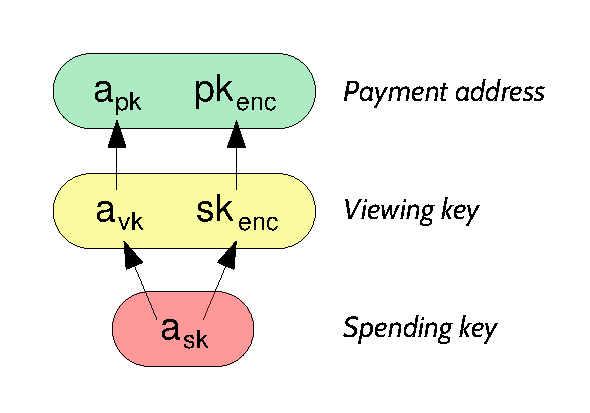
\includegraphics[scale=.7,interpolate]{key_components}}
\sapling{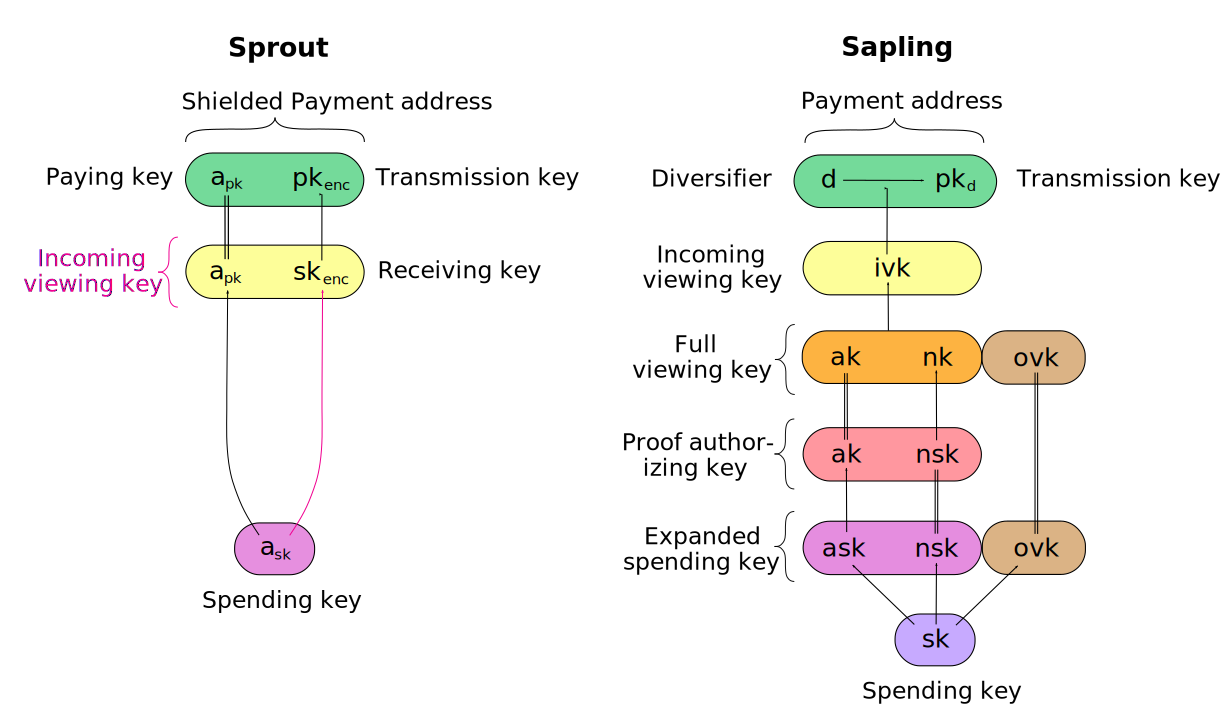
\includegraphics[scale=.5,interpolate]{key_components_sapling}}
\end{center}

\sproutspecific{
The \receivingKey $\TransmitPrivate$, the \incomingViewingKey
$\InViewingKey = (\AuthPublic, \TransmitPrivate)$, and the \paymentAddress
$\PaymentAddress = (\AuthPublic, \TransmitPublic)$ are derived from
$\AuthPrivate$, as described in \crossref{sproutkeycomponents}.
} %sproutspecific

\saplingonward{
The \authSigningKey $\AuthSignPrivate$,
the \authProvingKey $(\AuthSignPublic, \AuthProvePrivate)$,
the \fullViewingKey $(\AuthSignPublic, \AuthProvePublic)$,
the \incomingViewingKey $\InViewingKey$, and
each \diversifiedPaymentAddress $\DiversifiedPaymentAddress = (\Diversifier, \DiversifiedTransmitPublic)$
are derived from $\SpendingKey$, as described in \crossref{saplingkeycomponents}.
} %saplingonward

The composition of \paymentAddresses, \changed{\incomingViewingKeys,}
\sapling{\fullViewingKeys,} and \spendingKeys is a cryptographic protocol
detail that should not normally be exposed to users. However, user-visible
operations should be provided to obtain a
\paymentAddress\changed{ or \incomingViewingKey}\sapling{ or \fullViewingKey}
from a \spendingKey.

Users can accept payment from multiple parties with a single \paymentAddress
and the fact that these payments are destined to
the same payee is not revealed on the \blockchain, even to the
paying parties. \emph{However} if two parties collude to compare a
\paymentAddress they can trivially determine they are the same. In the
case that a payee wishes to prevent this they should create a distinct
\paymentAddress for each payer.

\saplingonward{
\Sapling provides a mechanism to allow the efficient creation of
\diversifiedPaymentAddresses with the same spending authority. A group of
such addresses shares the same \fullViewingKey and \incomingViewingKey, and
so creating as many unlinkable addresses as needed does not increase the cost
of scanning the \blockchain for relevant \transactions.
} %saplingonward

\vspace{-1ex}
\pnote{
It is conventional in cryptography to refer to the key used to encrypt
a message in an asymmetric encryption scheme as the \quotedterm{public key}.
However, the public key used as the \transmissionKey component of an address
($\TransmitPublic$\sapling{ or $\DiversifiedTransmitPublic$}) need not be
publically distributed; it has the same distribution as the \paymentAddress itself.
As mentioned above, limiting the distribution of the \paymentAddress is important
for some use cases. This also helps to reduce reliance of the overall protocol
on the security of the cryptosystem used for \note encryption
(see \crossref{inband}), since an adversary would have to know
$\TransmitPublic$\sapling{ or some $\DiversifiedTransmitPublic$} in order to
exploit a hypothetical weakness in that cryptosystem.
}

\introsection
\subsection{\Notes} \label{notes}

\sprout{
A \note (denoted $\NoteTuple{}$) is a tuple $\changed{(\AuthPublic, \Value,
\NoteAddressRand, \NoteCommitRand)}$. It represents that a value $\Value$ is
spendable by the recipient who holds the \spendingKey $\AuthPrivate$ corresponding
to $\AuthPublic$, as described in the previous section.
} %sprout
\notsprout{
A \note (denoted $\NoteTuple{}$) can be a \Sprout \note\sapling{ or a
\Sapling \note}. In either case it represents that a value $\Value$ is
spendable by the recipient who holds the \spendingKey corresponding
to a given \paymentAddress.
} %notsprout

\introlist
A \SproutOrNothing \note is a tuple $\changed{(\AuthPublic,
\Value, \NoteAddressRand, \NoteCommitRand)}$, where:
\begin{itemize}
  \item $\AuthPublic \typecolon \PRFOutput$ is the \payingKey of the
        recipient's \paymentAddress;
  \item $\Value \typecolon \range{0}{\MAXMONEY}$ is an integer
        representing the value of the \note in \zatoshi
        ($1$ \ZEC = $10^8$ \zatoshi);
  \item $\NoteAddressRand \typecolon \PRFOutput$
        is used as input to $\PRFnf{\AuthPrivate}$ to derive the
        \nullifier of the \note;
  \item $\NoteCommitRand \typecolon \NoteCommitSproutTrapdoor$
        is a random \commitmentTrapdoor as defined in \crossref{abstractcommit}.
\end{itemize}

\introlist
Let $\NoteTypeSprout$ be the type of a \SproutOrNothing \note, i.e.
\begin{formulae}
  \item $\NoteTypeSprout := \changed{\PRFOutput \times \range{0}{\MAXMONEY} \times \PRFOutput
           \times \NoteCommitSproutTrapdoor}$.
\end{formulae}

\sapling{
\vspace{1ex}
\introlist
A \Sapling \note is a tuple $(\Diversifier, \DiversifiedTransmitPublic,
\Value, \NoteCommitRand)$, where:
\begin{itemize}
  \item $\Diversifier \typecolon \DiversifierType$
        is the \diversifier of the recipient's \paymentAddress;
  \item $\DiversifiedTransmitPublic \typecolon \GroupJ$
        is the \diversifiedTransmissionKey of the recipient's \paymentAddress;
  \item $\Value \typecolon \range{0}{\MAXMONEY}$ is an integer
        representing the value of the \note in \zatoshi;
  \item $\NoteCommitRand \typecolon \NoteCommitSaplingTrapdoor$
        is a random \commitmentTrapdoor as defined in \crossref{abstractcommit}.
\end{itemize}

\introlist
Let $\NoteTypeSapling$ be the type of a \Sapling \note, i.e.
\begin{formulae}
  \item $\NoteTypeSapling := \DiversifierType \times \GroupJ \times \range{0}{\MAXMONEY}
           \times \NoteCommitSaplingTrapdoor$.
\end{formulae}
} %sapling

Creation of new \notes is described in \crossref{send}. When \notes are sent,
only a commitment (see \crossref{abstractcommit}) to the above values is disclosed
publically, and added to a data structure called the \noteCommitmentTree.
This allows the value and recipient to be kept private, while the commitment is
used by the \zeroKnowledgeProof when the \note is spent, to check that it exists
on the \blockchain.

\vspace{2ex}
\introlist
A \SproutOrNothing{} \noteCommitment on a \note
$\NoteTuple{} = \changed{(\AuthPublic, \Value, \NoteAddressRand, \NoteCommitRand)}$ is computed as

\begin{formulae}
  \item $\NoteCommitmentSprout(\NoteTuple{}) =
          \NoteCommitSprout{\NoteCommitRand}(\AuthPublic, \Value, \NoteAddressRand)$,
\end{formulae}
\vspace{-1.5ex}
where $\NoteCommitSprout{}$ is instantiated in \crossref{concretesproutcommit}.


\sapling{
\vspace{2ex}
\introlist
Let $\DiversifyHash$ be as defined in \crossref{concretediversifyhash}.

A \Sapling{} \noteCommitment on a \note
$\NoteTuple{} = (\Diversifier, \DiversifiedTransmitPublic, \Value, \NoteCommitRand)$ is computed as

\begin{formulae}
  \item $\DiversifiedTransmitBase := \DiversifyHash(\Diversifier)$
        \vspace{-1ex}
  \item $\NoteCommitmentSapling(\NoteTuple{}) := \begin{cases}
          \bot, &\caseif \DiversifiedTransmitBase = \bot \\
          \NoteCommitSapling{\NoteCommitRand}(\reprJOf{\DiversifiedTransmitBase},
                                              \reprJOf{\DiversifiedTransmitPublic},
                                              \Value), &\caseotherwise.
        \end{cases}$
\end{formulae}
\vspace{-1.5ex}
where $\NoteCommitSapling{}$ is instantiated in \crossref{concretewindowedcommit}.

Notice that the above definition of a \Sapling \note does not have a
$\NoteAddressRand$ field. There is in fact a $\NoteAddressRand$ value associated
with each \Sapling \note, but this only be computed once its position in the
\noteCommitmentTree is known (see \crossref{blockchain} and \crossref{transactions}).
We refer to the combination of a \note and its \notePosition $\NotePosition$, as a
\positionedNote.

For a \positionedNote, we can compute the value
$\NoteAddressRand \typecolon \bitseq{\PRFOutputLengthSapling}$; see
\crossref{commitmentsandnullifiers}.
} %sapling

\vspace{2ex}
A \nullifier (denoted $\nf$) is derived from the $\NoteAddressRand$ value
of a \note and the recipient's
\spendingKey $\AuthPrivate$\sapling{ or \nullifierKey $\AuthProvePublic$}.
This computation uses a \pseudoRandomFunction (see \crossref{abstractprfs}),
as described in \crossref{commitmentsandnullifiers}.

A \note is spent by proving knowledge of
$(\NoteAddressRand, \AuthPrivate)$\sapling{ or $(\NoteAddressRand, \AuthSignPublic, \AuthProvePrivate)$}
in zero knowledge while publically disclosing its \nullifier $\nf$,
allowing $\nf$ to be used to prevent double-spending. \sapling{In the case
of \Sapling, a \spendAuthSignature is also required, in order to demonstrate
knowledge of $\AuthSignPrivate$.}


\subsubsection{\NotePlaintexts{} and \Memos} \label{noteptconcept}

Transmitted \notes are stored on the \blockchain in encrypted form, together with
a \noteCommitment $\cm$.

The \notePlaintexts in a \joinSplitDescription are encrypted to the
respective \transmissionKeys $\TransmitPublicNew{\allNew}$.
Each \SproutOrNothing{} \notePlaintext (denoted $\NotePlaintext{}$) consists of
$(\Value, \NoteAddressRand, \NoteCommitRand\changed{, \Memo})$.

\saplingonward{
The \notePlaintext in each \outputDescription is encrypted to the
\diversifiedTransmissionKey $\DiversifiedTransmitPublic$.
Each \Sapling{} \notePlaintext (denoted $\NotePlaintext{}$) consists of
$(\Diversifier, \Value, \NoteCommitRand, \Memo)$.
} %saplingonward

\changed{
$\Memo$ represents a \memo associated with this \note. The usage of the
\memo is by agreement between the sender and recipient of the \note.
}

Other fields are as defined in \crossref{notes}.

Encodings are given in \crossref{notept}.

The result of encryption forms part of a \notesCiphertext (see \crossref{inband}
for further details).


\subsection{The Block Chain} \label{blockchain}

At a given point in time, each \fullValidator is aware of a set of candidate
\blocks. These form a tree rooted at the \genesisBlock, where each node
in the tree refers to its parent via the $\hashPrevBlock$ \blockHeader field
(see \crossref{blockheader}).

A path from the root toward the leaves of the tree consisting of a sequence
of one or valid \blocks consistent with consensus rules, is called a
\validBlockchain.

Each \block in a \blockchain has a \blockHeight. The \blockHeight of the
\genesisBlock is $0$, and the \blockHeight of each subsequent \block in the
\blockchain increments by $1$.

In order to choose the \bestValidBlockchain in its view of the
overall \block tree, a node sums the work, as defined in \crossref{workdef}, of
all \blocks in each chain, and considers the \validBlockchain with greatest
total work to be best. To break ties between leaf \blocks, a node will prefer the
\block that it received first.

The consensus protocol is designed to ensure that for any given \blockHeight,
the vast majority of nodes should eventually agree on their \bestValidBlockchain
up to that height.


\subsection{Transactions and Treestates} \label{transactions}

Each \block contains one or more \transactions.

Inputs to a \transaction insert value into a \transparentValuePool, and outputs
remove value from this pool. As in \Bitcoin, the remaining value in the pool is
available to miners as a fee.

\vspace{-3ex}
\consensusrule{
The remaining value in the \transparentValuePool{} \MUST be nonnegative.
}
\vspace{2ex}

\sprout{To each \transaction there is associated an initial \treestate.}
\notsprout{To each \transaction there are associated initial \treestates
for \Sprout\sapling{ and for \Sapling}.}

\introlist
\sprout{A}\sapling{Each} \treestate consists of:

\begin{itemize}
  \item a \noteCommitmentTree (\crossref{merkletree});
  \item a \nullifierSet (\crossref{nullifierset}).
\end{itemize}

Validation state associated with \transparentTransfers, such as the UTXO
(Unspent Transaction Output) set, is not described in this document; it is
used in essentially the same way as in \Bitcoin.

An \anchor is a Merkle tree root of a \noteCommitmentTree\sapling{ (either the
\Sprout tree or the \Sapling tree)}. It uniquely identifies a \noteCommitmentTree
state given the assumed security properties of the Merkle tree's
\hashFunction. Since the \nullifierSet is always updated together with the
\noteCommitmentTree, this also identifies a particular state of the associated
\nullifierSet.

\introlist
In a given \blockchain, \sapling{for each of \Sprout and \Sapling,}
\treestates are chained as follows:

\begin{itemize}
  \item The input \treestate of the first \block is the empty \treestate.
  \item The input \treestate of the first \transaction of a \block is the final
        \treestate of the immediately preceding \block.
  \item The input \treestate of each subsequent \transaction in a \block is the
        output \treestate of the immediately preceding \transaction.
  \item The final \treestate of a \block is the output \treestate of its last
        \transaction.
\end{itemize}

\joinSplitDescriptions also have interstitial input and output
\treestates\notsprout{ for \Sprout}, explained in the following section.
\sapling{There is no equivalent of interstitial \treestates for \Sapling.}


\subsection{\JoinSplitTransfers{} and Descriptions} \label{joinsplit}

A \joinSplitDescription is data included in a \transaction that describes a \joinSplitTransfer,
i.e.\ a \shielded value transfer.
\sprout{This kind of value transfer is}
\notsprout{In \Sprout, this kind of value transfer was}
the primary \Zcash-specific operation performed by \transactions.

A \joinSplitTransfer spends $\NOld$ \notes $\nOld{\allOld}$ and \transparent input
$\vpubOld$, and creates $\NNew$ \notes $\nNew{\allNew}$ and \transparent output
$\vpubNew$.
It is associated with a \joinSplitStatement instance (\crossref{joinsplitstatement}),
for which it provides a \zkSNARKProof{}.

Each \transaction has a \sequenceOfJoinSplitDescriptions{}.

The \changed{total $\vpubNew$ value adds to, and the total} $\vpubOld$
value subtracts from the \transparentValuePool of the containing \transaction.

The \anchor of each \joinSplitDescription in a \transaction{} refers to a
\SproutOrNothing \treestate.

For each of the $\NOld$ \shieldedInputs, a \nullifier is revealed. This allows
detection of double-spends as described in \crossref{nullifierset}.

\changed{
For each \joinSplitDescription in a \transaction, an interstitial output \treestate is
constructed which adds the \noteCommitments and \nullifiers specified in that
\joinSplitDescription to the input \treestate referred to by its \anchor.
This interstitial output \treestate is available for use as the \anchor of subsequent
\joinSplitDescriptions in the same \transaction.

Interstitial \treestates are necessary because when a \transaction is constructed,
it is not known where it will eventually appear in a mined \block. Therefore the
\anchors that it uses must be independent of its eventual position.
}

\begin{consensusrules}
  \item The input and output values of each \joinSplitTransfer{} \MUST balance
        exactly.
  \item For the first \joinSplitDescription of a \transaction, the \anchor \MUST
        be the output \SproutOrNothing \treestate of a previous \block.
\changed{
  \item The \anchor of each \joinSplitDescription in a \transaction{} \MUST refer
        to either some earlier \block's final \SproutOrNothing \treestate, or to
        the interstitial output \treestate of any prior \joinSplitDescription in
        the same \transaction.
}
\end{consensusrules}


\sapling{
\subsection{\SpendTransfers, \OutputTransfers, and their Descriptions} \label{spendsandoutputs}

\joinSplitTransfers are not used for \Sapling \notes. Instead, there is a
separate \spendTransfer for each \shieldedInput, and a separate \outputTransfer
for each \shieldedOutput.

\spendDescriptions and \outputDescriptions are data included in a transaction
that describe \spendTransfers and \outputTransfers, respectively.

A \spendTransfer spends a \note $\nOld{}$. Its \spendDescription includes a
\xPedersenValueCommitment to the value of the \note.
It is associated with an instance of a \spendStatement (\crossref{spendstatement})
for which it provides a \zkSNARKProof{}.

An \outputTransfer creates a \note $\nNew{}$. Similarly, its \outputDescription
includes a \xPedersenValueCommitment to the \note value.
It is associated with an instance of an \outputStatement (\crossref{outputstatement})
for which it provides a \zkSNARKProof{}.

Each \transaction has a sequence of \spendDescriptions and a sequence of
\outputDescriptions.

To ensure balance, we use a homomorphic property of \xPedersenCommitments that
allows them to be added and subtracted, as elliptic curve points. The result
of adding two \xPedersenValueCommitments, committing to values $\Value_1$ and
$\Value_2$, is a new \xPedersenValueCommitment that commits to $\Value_1 + \Value_2$.
Subtraction works similarly.

Therefore, balance can be enforced by adding all of the \valueCommitments for
\shieldedInputs, subtracting all of the \valueCommitments for \shieldedOutputs,
and checking that the result commits to a value consistent with the net \transparent
value change (see \crossref{saplingbalance} for a full specification).
This approach allows all of the \zkSNARK statements to be independent of
each other, potentially increasing opportunities for precomputation.

A \spendDescription includes an \anchor, which refers to the output
\Sapling \treestate of a previous \block. It also reveals a \nullifier,
which allows detection of double-spends as described in \crossref{nullifierset}.

\pnote{
Interstitial \treestates are not necessary for \Sapling, because a \spendTransfer
in a given \transaction cannot spend any of the \shieldedOutputs of the same
\transaction. This is not an onerous restriction because, unlike \Sprout where
each \joinSplitTransfer must balance individually, in \Sapling it is only necessary
for the whole \transaction to balance.
}

\begin{consensusrules}
  \item The \transaction{} \MUST balance as specified in \crossref{saplingbalance}.
  \item The \anchor of each \spendDescription in a \transaction{} \MUST refer
        to some earlier \block's final \Sapling \treestate.
\end{consensusrules}
} %sapling


\subsection{\NoteCommitmentTrees} \label{merkletree}

\begin{center}
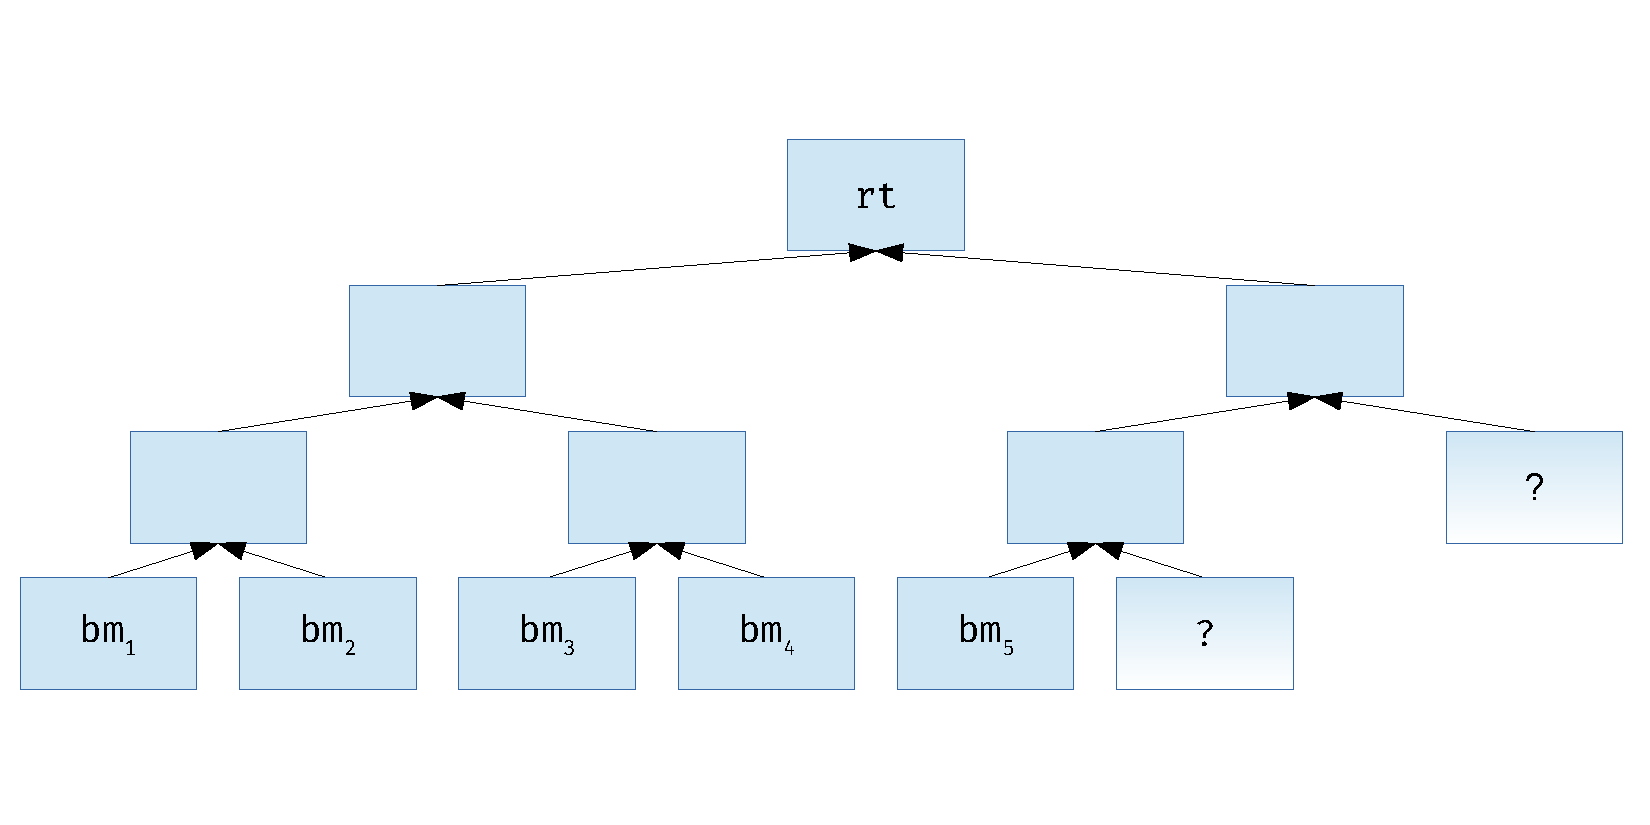
\includegraphics[scale=.4,interpolate]{incremental_merkle}
\end{center}

\sapling{\todo{The commitment indices in the above diagram should be zero-based to reflect the \notePosition{}.}}

The \noteCommitmentTree is an \incrementalMerkleTree of fixed depth used to store
\noteCommitments that \joinSplitTransfers\sapling{ and \spendTransfers} produce.
Just as the \term{unspent transaction output set} (UTXO set) used in \Bitcoin,
it is used to express the existence of value and the capability to spend it.
However, unlike the UTXO set, it is \emph{not} the job of this tree to protect
against double-spending, as it is append-only.

A \merkleRoot of this tree is associated with each \treestate, as described in
\crossref{transactions}.

Each \merkleNode in the \incrementalMerkleTree is associated with a \merkleHash of
size $\MerkleHashLengthSprout$ \sapling{ or $\MerkleHashLengthSapling$} bits.
The \merkleLayer numbered $h$, counting from \merkleLayer $0$ at the \merkleRoot, has
$2^h$ \merkleNodes with \merkleIndices $0$ to $2^h-1$ inclusive.
The \merkleHash associated with the \merkleNode at \merkleIndex $i$ in \merkleLayer $h$
is denoted $\MerkleNode{h}{i}$.


\subsection{\NullifierSets} \label{nullifierset}

Each \fullValidator maintains a \nullifierSet logically associated with each \treestate.
As valid \transactions containing \joinSplitTransfers \sapling{ or \spendTransfers} are
processed, the \nullifiers revealed in \joinSplitDescriptions \sapling{ and \spendDescriptions}
are inserted into the \nullifierSet associated with the new \treestate.

\xNullifiers are enforced to be unique within a \validBlockchain, in order to
prevent double-spends.

\consensusrule{
A \nullifier{} \MUSTNOT repeat either within a \transaction, or across
\transactions in a \validBlockchain.
}

\sapling{\pnote{
\Sprout and \Sapling \nullifiers are considered disjoint, even if they have
the same bit pattern.
}}


\subsection{Block Subsidy and Founders' Reward} \label{subsidyconcepts}

Like \Bitcoin, \Zcash creates currency when \blocks are mined. The value created on
mining a \block is called the \blockSubsidy. It is composed of a \minerSubsidy and a
\foundersReward. As in \Bitcoin, the miner of a \block also receives \transactionFees.

The calculations of the \blockSubsidy, \minerSubsidy, and \foundersReward depend on
the \blockHeight, as defined in \crossref{blockchain}.

These calculations are described in \crossref{subsidies}.


\subsection{\CoinbaseTransactions}

The first \transaction in a block must be a \coinbaseTransaction, which should
collect and spend any \minerSubsidy and \transactionFees paid by \transactions
included in this \block. The \coinbaseTransaction must also pay the \foundersReward
as described in \crossref{foundersreward}.


\intropart
\section{Abstract Protocol}

\subsection{Abstract Cryptographic Schemes}

\subsubsection{\HashFunctions} \label{abstracthashes}

Let $\MerkleDepthSprout$, $\MerkleHashLengthSprout$,
\sapling{$\MerkleDepthSapling$, $\MerkleHashLengthSapling$, $\InViewingKeyLength$,}
$\RandomSeedLength$, $\hSigLength$, $\PRFOutputLength$, and $\NOld$
be as defined in \crossref{constants}.

\sapling{Let $\ellJ$ be as defined in \crossref{jubjub}.}

\sprout{
$\MerkleCRH \typecolon \MerkleHashSprout \times \MerkleHashSprout \rightarrow \MerkleHashSprout$
is a \collisionResistant \hashFunction used in \crossref{merklepath}.
It is instantiated in \crossref{merklecrh}.
} %sprout
\notsprout{
The functions $\MerkleCRHSprout \typecolon \MerkleLayerSprout \times \MerkleHashSprout \times \MerkleHashSprout
\rightarrow \MerkleHashSprout$
\sapling{and (for \Sapling),
$\MerkleCRHSapling \typecolon \MerkleLayerSapling \times \MerkleHashSapling \times \MerkleHashSapling
\rightarrow \MerkleHashSapling$
}
are \hashFunctions used in \crossref{merklepath}.
\sapling{$\MerkleCRHSapling$ is \collisionResistant on all its arguments, and}
$\MerkleCRHSprout$ is \collisionResistant except on its first argument.
Both of these functions are instantiated in \crossref{merklecrh}.
} %notsprout

\changed{
$\hSigCRH{} \typecolon \bitseq{\RandomSeedLength} \times \typeexp{\PRFOutput}{\NOld} \times \JoinSplitSigPublic \rightarrow \hSigType$
is a \collisionResistant \hashFunction used in \crossref{joinsplitdesc}.
It is instantiated in \crossref{hsigcrh}.

$\EquihashGen{} \typecolon (n \typecolon \PosInt) \times \PosInt \times \byteseqs \times \PosInt \rightarrow \bitseq{n}$
is another \hashFunction, used in \crossref{equihash} to generate
input to the Equihash solver. The first two arguments, representing
the Equihash parameters $n$ and $k$, are written subscripted.
It is instantiated in \crossref{equihashgen}.
}

\sapling{
$\CRHivk \typecolon \ReprJ \times \ReprJ \rightarrow \binaryrange{\InViewingKeyLength}$
is a \collisionResistant \hashFunction used in \crossref{saplingkeycomponents}
to derive an \incomingViewingKey for a \Sapling \paymentAddress. It is also used
in the \spendStatement (\crossref{spendstatement}) to confirm use of the correct
key for the \note being spent. It is instantiated in \crossref{concretecrhivk}.

$\DiversifyHash \typecolon \DiversifierType \rightarrow \GroupJ$ is a \hashFunction
satisfying the Discrete Logarithm Independence property (which implies \collisionResistance\!\!)
described in \crossref{abstractgrouphash}.
It is used to derive a \diversifiedBase from a \diversifier in \crossref{saplingkeycomponents}.
It is instantiated in \crossref{concretediversifyhash}.
} %sapling


\introsection
\subsubsection{\PseudoRandomFunctions} \label{abstractprfs}

$\PRF{x}{}$ is a \pseudoRandomFunction keyed by $x$.

Let $\AuthPrivateLength$, $\NoteAddressPreRandLength$, $\hSigLength$,
$\PRFOutputLengthSprout$, \sapling{$\PRFOutputLengthSapling$,} $\NOld$, and $\NNew$
be as defined in \crossref{constants}.

\sapling{Let $\ellJ$ and $\ParamJ{r}$ be as defined in \crossref{jubjub}.}

\sprout{\changed{Four} \emph{independent} $\PRF{x}{}$ are needed in our protocol:}

\notsprout{For \Sprout, \changed{four} \emph{independent} $\PRF{x}{}$ are needed:}

\begin{tabular}{@{\hskip 2em}l@{\notsprout{\hskip 1.88em}}l@{\;}l@{\;}l@{\;}l}
$\PRFaddr{}      $&$\typecolon\; \bitseq{\AuthPrivateLength} $&$\times\; \byte $& &$\rightarrow \PRFOutput $\\
$\PRFnf{}        $&$\typecolon\; \bitseq{\AuthPrivateLength} $&$\times\; \PRFOutput $& &$\rightarrow \PRFOutput $\\
$\PRFpk{}        $&$\typecolon\; \bitseq{\AuthPrivateLength} $&$\times\; \setofOld $&$\times\; \hSigType $&$\rightarrow \PRFOutput $\\
$\PRFrho{}       $&$\typecolon\; \bitseq{\NoteAddressPreRandLength} $&$\times\; \setofNew $&$\times\; \hSigType $&$\rightarrow \PRFOutput $
\end{tabular}

These are used in \crossref{joinsplitstatement}; $\PRFaddr{}$ is also used to
derive a \paymentAddress from a \spendingKey in \crossref{sproutkeycomponents}.

\sapling{
For \Sapling, two additional $\PRF{x}{}$ are needed:

\begin{tabular}{@{\hskip 2em}l@{\;}l@{\hskip 0.6em}l@{\;}l@{\hskip 4.25em}l}
$\PRFexpand{}    $&$\typecolon\; \bitseq{\SpendingKeyLength} $&$\times\; \byte  $& &$\rightarrow \GF{\ParamJ{r}} $\\
$\PRFnfSapling{} $&$\typecolon\; \ReprJ                      $&$\times\; \ReprJ $& &$\rightarrow \PRFOutputSapling $
\end{tabular}

$\PRFexpand{}$ is used in \crossref{saplingkeycomponents}.

$\PRFnfSapling{}$ is used in \crossref{spendstatement}.
} %sapling

\sprout{They}\notsprout{All of these \pseudoRandomFunctions} are instantiated in \crossref{concreteprfs}.

\begin{securityrequirements}
  \item Security definitions for \pseudoRandomFunctions are given in \cite[section 4]{BDJR2000}.
  \item In addition to being \pseudoRandomFunctions, it is required that
        $\PRFnf{x}$,\changed{ $\PRFaddr{x}$,\sprout{ and} $\PRFrho{x}$}\sapling{, and $\PRFnfSapling{x}$}
        be \collisionResistant across all $x$ --- i.e.\ finding $(x, y) \neq (x', y')$
        such that $\PRFnf{x}(y) = \PRFnf{x'}(y')$ should not be feasible\changed{, and
        similarly for $\PRFaddr{}$ and $\PRFrho{}$\sapling{ and $\PRFnfSapling{}$}}.
\end{securityrequirements}

\pnote{$\PRFnf{}$ was called $\PRFsn{}$ in \Zerocash \cite{BCG+2014}.}


\introsection
\subsubsection{\SymmetricEncryption} \label{abstractsym}

Let $\Sym$ be an \symmetricEncryptionScheme with keyspace $\Keyspace$, encrypting
plaintexts in $\Plaintext$ to produce ciphertexts in $\Ciphertext$.

$\SymEncrypt{} \typecolon \Keyspace \times \Plaintext \rightarrow \Ciphertext$
is the encryption algorithm.

$\SymDecrypt{} \typecolon \Keyspace \times \Ciphertext \rightarrow
\Plaintext \union \setof{\bot}$ is the corresponding decryption algorithm, such that
for any $\Key \in \Keyspace$ and $\Ptext \in \Plaintext$,
$\SymDecrypt{\Key}(\SymEncrypt{\Key}(\Ptext)) = \Ptext$.
$\bot$ is used to represent the decryption of an invalid ciphertext.

\securityrequirement{
$\Sym$ must be one-time (INT-CTXT $\wedge$ IND-CPA)-secure. \quotedterm{One-time} here
means that an honest protocol participant will almost surely encrypt only one message
with a given key; however, the attacker may make many adaptive chosen ciphertext
queries for a given key. The security notions INT-CTXT and IND-CPA are as defined in
\cite{BN2007}.
}

\subsubsection{\KeyAgreement} \label{abstractkeyagreement}

A \keyAgreementScheme is a cryptographic protocol in which two parties agree
a shared secret, each using their private key and the other party's public key.

A \keyAgreementScheme $\KA$ defines a type of public keys $\KAPublic$, a type
of private keys $\KAPrivate$, and a type of shared secrets $\KASharedSecret$.

Let $\KAFormatPrivate \typecolon \PRFOutput \rightarrow \KAPrivate$ be a function
that converts a bit string of length $\PRFOutputLength$ to a $\KA$ private key.

Let $\KADerivePublic \typecolon \KAPrivate \times \KAPublic \rightarrow \KAPublic$
be a function that derives the $\KA$ public key corresponding to a given $\KA$
private key and base point.

Let $\KAAgree \typecolon \KAPrivate \times \KAPublic \rightarrow \KASharedSecret$
be the agreement function.

\sapling{Optional:} Let $\KABase \typecolon \KAPublic$ be a public base point.

\pnote{
The range of $\KADerivePublic$ may be a strict subset of $\KAPublic$.
}

\begin{securityrequirements}
  \item $\KAFormatPrivate$ must preserve sufficient entropy from its input to be used
        as a secure $\KA$ private key.
  \item The key agreement and the KDF defined in the next section must together
        satisfy a suitable adaptive security assumption along the lines of
        \cite[section 3]{Bern2006} or \cite[Definition 3]{ABR1999}.
\end{securityrequirements}

More precise formalization of these requirements is beyond the scope of this
specification.


\subsubsection{\KeyDerivation} \label{abstractkdf}

A \keyDerivationFunction is defined for a particular \keyAgreementScheme and
\symmetricEncryptionScheme; it takes the shared secret produced by the key
agreement and additional arguments, and derives a key suitable for the encryption
scheme.

Let $\KDF \typecolon \setofNew \times \hSigType \times \KASharedSecret
\times \KAPublic \times \KAPublic \rightarrow \Keyspace$ be a
\keyDerivationFunction suitable for use with $\KA$, deriving keys
for $\SymEncrypt{}$.

\securityrequirement{
In addition to adaptive security of the key agreement and KDF,
the following security property is required:

\notsprout{
\todo{adapt this definition to handle \Sapling, or maybe just remove it.}

Let $\TransmitBase := \todo{?}$
}
\sprout{Let $\TransmitBase := \KABase$.}

Let $\TransmitPrivateSup{1}$ and $\TransmitPrivateSup{2}$ each be chosen uniformly and
independently at random from $\KAPrivate$.

Let $\TransmitPublicSup{j} := \KADerivePublic(\TransmitPrivateSup{j}, \TransmitBase)$.

\introlist
An adversary can adaptively query a function
$Q \typecolon \range{1}{2} \times \hSigType \rightarrow
\KAPublic \times \Keyspace_{\allNew}$ where $Q_j(\hSig)$ is defined as follows:
\begin{enumerate}
  \item Choose $\EphemeralPrivate$ uniformly at random from $\KAPrivate$.
  \item Let $\EphemeralPublic := \KADerivePublic(\EphemeralPrivate, \TransmitBase)$.
  \item For $i \in \setofNew$, let $\Key_i :=
        \KDF(i, \hSig, \KAAgree(\EphemeralPrivate, \TransmitPublicSup{j}), \EphemeralPublic, \TransmitPublicSup{j}))$.
  \item Return $(\EphemeralPublic, \Key_{\allNew})$.
\end{enumerate}

Then the adversary must make another query to $Q_j$ with random unknown
$j \in \range{1}{2}$, and guess $j$ with probability greater than chance.
}

If the adversary's advantage is insignificant, then the asymmetric encryption scheme
constructed from $\KA$, $\KDF$ and $\Sym$ in \crossref{inband} will be key-private
as defined in \cite{BBDP2001}.

\pnote{The given definition only requires ciphertexts to be indistinguishable
between \transmissionKeys that are outputs of $\KADerivePublic$ (which
includes all keys generated as in \crossref{sproutkeycomponents}). If a
\transmissionKey not in that range is used, it may be distinguishable.
This is not considered to be a significant security weakness.
}


\introlist
\subsubsection{Signature} \label{abstractsig}

A signature scheme $\Sig$ defines:

\begin{itemize}
  \item a type of signing keys $\SigPrivate$;
  \item a type of verifying keys $\SigPublic$;
  \item a type of messages $\SigMessage$;
  \item a type of signatures $\SigSignature$;
  \item a randomized key pair generation algorithm $\SigGen \typecolon () \rightarrowR \SigPrivate \times \SigPublic$;
  \item a randomized signing algorithm $\SigSign{} \typecolon \SigPrivate \times \SigMessage \rightarrowR \SigSignature$;
  \item a verifying algorithm $\SigVerify{} \typecolon \SigPublic \times \SigMessage \times \SigSignature \rightarrow \bit$;
\end{itemize}

such that for any key pair $(\sk, \vk) \leftarrowR \SigGen()$, and
any $m \typecolon \SigMessage$ and $s \typecolon \SigSignature \leftarrowR \SigSign{\sk}(m)$,
$\SigVerify{\vk}(m, s) = 1$.

\vspace{2ex}
\introlist
\Zcash uses \sprout{two}\sapling{three} signature schemes:

\begin{itemize}
  \item one used for signatures that can be verified by script operations such as
        \ScriptOP{CHECKSIG} and \ScriptOP{CHECKMULTISIG} as in \Bitcoin;
  \item one called $\JoinSplitSig$ (instantiated in \crossref{concretejssig}),
        which is used to sign \transactions that contain at least one
        \joinSplitDescription\sprout{.}\notsprout{;}
  \saplingonwarditem{one called $\SpendAuthSig$ (instantiated in
        \crossref{concretespendauthsig}), which is used to sign authorizations of
        \spendDescriptions.}
\end{itemize}

The following defines only the security properties needed for $\JoinSplitSig$.
\sapling{Security properties for $\SpendAuthSig$ are defined in the next section,
\crossref{abstractsigrerand}.}

\securityrequirement{
$\JoinSplitSig$ must be Strongly Unforgeable under (non-adaptive) Chosen Message Attack
(SU-CMA), as defined for example in \cite[Definition 6]{BDEHR2011}. This allows an
adversary to obtain signatures on chosen messages, and then requires it to be infeasible
for the adversary to forge a previously unseen valid \mbox{(message, signature)}
pair without access to the signing key.
}

\todo{Reference a different paper for the security definition. \cite{BDEHR2011} has
a flawed security proof; this doesn't affect \Zcash but it would be better to avoid
confusion that it might.}

\begin{pnotes}
  \item A fresh signature key pair is generated for each \transaction containing
        a \joinSplitDescription{}.
        Since each key pair is only used for one signature (see \crossref{nonmalleability}),
        a one-time signature scheme would suffice for $\JoinSplitSig$.
        This is also the reason why only security against \emph{non-adaptive}
        chosen message attack is needed. In fact the instantiation of $\JoinSplitSig$
        uses a scheme designed for security under adaptive attack even when multiple
        signatures are signed under the same key.
  \item SU-CMA security requires it to be infeasible for the adversary, not
        knowing the private key, to forge a distinct signature on a previously
        seen message. That is, \joinSplitSignatures are intended to be nonmalleable
        in the sense of \cite{BIP-62}.
\end{pnotes}


\sapling{
\introlist
\subsubsubsection{Signature with Re-Randomizable Keys} \label{abstractsigrerand}

A \rerandomizableSignatureScheme $\Sig$ is a \signatureScheme that
additionally defines:

\begin{itemize}
  \item a type of randomizers $\SigRandom$;
  \item a public key randomization algorithm $\SigRandomizePublic \typecolon \SigPublic \times \SigRandom \rightarrow \SigPublic$;
  \item a private key randomization algorithm $\SigRandomizePrivate \typecolon \SigPrivate \times \SigRandom \rightarrow \SigPrivate$
  \item a distinguished ``identity'' randomizer $\SigRandomnessId \typecolon \SigRandom$
\end{itemize}

\vspace{-1.2ex}
such that if $(\pk \typecolon \SigPublic, \sk \typecolon \SigPrivate)$ is a
valid $\Sig$ key pair, then:
\vspace{0.8ex}

\begin{itemize}
  \item $\left(\SigRandomizePublic(\pk, \SigRandomness), \SigRandomizePrivate(\sk, \SigRandomness)\right)$
        is also a valid $\Sig$ key pair for any $\SigRandomness \typecolon \SigRandom$;
  \item $\SigRandomizePrivate(\paramdot, \SigRandomness) \typecolon \SigPrivate \rightarrow \SigPrivate$
        is injective and easily invertible for any $\SigRandomness \typecolon \SigRandom$;
  \item For \emph{any} key pair $(\pk, \sk)$ returned by $\SigGen()$, the distribution of
        \begin{formulae}
          \item $\left(\SigRandomizePublic(\pk, \SigRandomness), \SigRandomizePrivate(\sk, \SigRandomness)\right) :
                \SigRandomness \leftarrowR \SigRandom$
        \end{formulae}
        \vspace{-0.5ex} is identical to the distribution of $\SigGen()$.
  \item $\left(\SigRandomizePublic(\pk, \SigRandomnessId), \SigRandomizePrivate(\sk, \SigRandomnessId)\right) = (\pk, \sk)$.
\end{itemize}

The following security requirement for such \signatureSchemes is based on that
given in \cite[section 3]{FKMSSS2016}. Note that we require Strong Unforgeability
with Re-randomized Keys, not Existential Unforgeability with Re-randomized Keys
(the latter is called ``Unforgeability under Re-randomized Keys'' in
\cite[Definition 8]{FKMSSS2016}). Unlike the case for $\JoinSplitSig$, we require
security under adaptive chosen message attack with multiple messages signed using
a given key. (Although each \note uses a different re-randomized key pair, the same
original key pair can be re-randomized for multiple \notes, and also it can happen
that multiple \transactions spending the same \note are revealed to an adversary.)

\introsection
\securityrequirement{\textbf{Strong Unforgeability with Re-randomized Keys under adaptive Chosen Message Attack (SURK-CMA)}

Let $\Oracle \typecolon \SigPrivate \times \SigMessage \times \SigRandom \rightarrow \SigSignature$
be a generator of signing oracles.

A signing oracle $\Oracle_{\sk}$ for private key $\sk$ has state
$Q \typecolon \powerset{\SigMessage \times \SigSignature}$ initialized to $\setof{}$
that records queried messages and corresponding signatures.

\begin{formulae}
  \item $\Oracle_{\sk} :=$ var $Q \leftarrow \setof{}$ in $\fun{(m \typecolon \SigMessage, \SigRandomness \typecolon \SigRandom)}{}$
  \item \tab let $\sigma = \SigSign{\SigRandomizePrivate(\sk, \SigRandomness)}(m)$
  \item \tab $Q \leftarrow Q \union \setof{(m, \sigma)}$
  \item \tab return $\sigma \typecolon \SigSignature$.
\end{formulae}

For random $(\pk, \sk) \leftarrowR \SigGen()$, it must be infeasible for an adversary
given $\pk$ and a new instance of $\Oracle_{\sk}$ to find $(m^*, \sigma^*, \SigRandomness^*)$
such that $\SigVerify{\SigRandomizePublic(\pk, \SigRandomness^*)}(m^*, \sigma^*) = 1$ and
$(m^*, \sigma^*) \not\in \Oracle_{\sk}\mathsf{.}Q$.
}

\begin{pnotes}
  \item The requirement for $\SigRandomnessId$ simplifies the definition of SURK-CMA
        by removing the need for two oracles (since the oracle for original keys,
        called $\Oracle_1$ in \cite{FKMSSS2016}, is a special case of the oracle for
        randomized keys).
  \item Since
        $\left(\SigRandomizePublic(\pk, \SigRandomness), \SigRandomizePrivate(\sk, \SigRandomness)\right) :
        \SigRandomness \leftarrowR \SigRandom$ is identically distributed to $\SigGen()$,
        the combination of a re-randomized public key and signature(s)
        under that key do not reveal the key from which it was re-randomized.
  \item Since $\SigRandomizePrivate(\paramdot, \SigRandomness)$ is injective and
        easily invertible, knowledge of $\SigRandomizePrivate(\sk, \SigRandomness)$
        \emph{and} $\SigRandomness$ implies knowledge of $\sk$.
\end{pnotes}
} %sapling


\introlist
\subsubsection{Commitment} \label{abstractcommit}

A \commitmentScheme is a function that, given a random \commitmentTrapdoor
and an input, can be used to commit to the input in such a way that:

\begin{itemize}
  \item no information is revealed about it without the \trapdoor (\quotedterm{hiding}),
  \item given the \trapdoor and input, the commitment can be verified to \quotedterm{open}
        to that input and no other (\quotedterm{binding}).
\end{itemize}

\vspace{-3ex}
A \commitmentScheme $\CommitAlg$ defines a type of inputs $\CommitInput$,
a type of commitments $\CommitOutput$, and a type of \commitmentTrapdoors
$\CommitTrapdoor$.

\vspace{2ex}
Let $\CommitAlg \typecolon \CommitTrapdoor \times \CommitInput \rightarrow \CommitOutput$
be a function satisfying the following security requirements.

\vspace{-2ex}
\begin{securityrequirements}
  \item \textbf{Computational hiding:} For all $x, x' \typecolon \CommitInput$,
        the distributions $\{\; \Commit{r}(x) \;|\; r \leftarrowR \CommitTrapdoor \;\}$
        and $\{\; \Commit{r}(x') \;|\; r \leftarrowR \CommitTrapdoor \;\}$ are
        computationally indistinguishable.
  \item \textbf{Computational binding:} It is infeasible to find
        $x, x' \typecolon \CommitInput$ and
        $r, r' \typecolon \CommitTrapdoor$
        such that $x \neq x'$ and $\Commit{r}(x) = \Commit{r'}(x')$.
\end{securityrequirements}

\vspace{-2ex}
\pnote{
If it were only feasible to find $x \typecolon \CommitInput$ and
$r, r' \typecolon \CommitTrapdoor$ such that $r \neq r'$ and
$\Commit{r}(x) = \Commit{r'}(x)$, this would not by itself contradict
the computational binding security requirement.
}


\introsection
\subsubsection{\RepresentedGroup} \label{abstractgroup}

A \representedGroup $\GroupG{}$ consists of:

\begin{itemize}
  \item a subgroup order parameter $\ParamG{r} \typecolon \PosInt$, which must be prime;
  \item a cofactor parameter $\ParamG{h} \typecolon \PosInt$;
  \item a group $\GroupG{}$ of order $\ParamG{h} \mult \ParamG{r}$, written additively
        with operation $+ \typecolon \GroupG{} \times \GroupG{} \rightarrow \GroupG{}$,
        and additive identity $\ZeroG{}$;
  \item a generator $\GenG{}$ of the subgroup of $\GroupG{}$ of order $\ParamG{r}$;
  \item a bit-length parameter $\ellG{} \typecolon \Nat$;
  \item a representation function \smash{$\reprG{} \typecolon \GroupG{} \rightarrow \bitseq{\ellG{}}$}
        and an abstraction function \smash{$\abstG{} \typecolon \bitseq{\ellG{}} \rightarrow \GroupG{} \union \setof{\bot}$},
        such that $\abstG{}$ is the left inverse of $\reprG{}$, i.e. for all $P \in \GroupG{}$,
        $\abstG{}(\reprG{}(P)) = P$, and for all $S$ not in the image of $\reprG{}$, $\abstG{}(S) = \bot$.
\end{itemize}
\vspace{-1.5ex}

% Do we actually need \GenG? It is natural to include it for some groups
% and not others.

For $G \typecolon \GroupG{}$ we write $-G$ for the negation of $G$, such that
$(-G) + G = \ZeroG{}$. We write $G - H$ for $G + (-H)$.

We also extend the $\vsum{}{}$ notation to addition on group elements.

For $G \typecolon \GroupG{}$ and $k \typecolon \Int$ we write $\scalarmult{k}{G}$
for scalar multiplication on the group, i.e.

\begin{formulae}
  \item $\scalarmult{k}{G} := \begin{cases}
          \ssum{i = 1}{k} G, &\caseif k \geq 0 \\[1.5ex]
          \ssum{i = 1}{-k} (-G), &\caseotherwise.
        \end{cases}$
\end{formulae}

For $G \typecolon \GroupG{}$ and $a \typecolon \GF{\ParamG{r}}$, we may also write
$\scalarmult{a}{G}$ meaning $\scalarmult{a \bmod \ParamG{r}}{G}$ as defined above.
(This variant is not defined for fields other than $\GF{\ParamG{r}}$.)


\sapling{
\introsection
\subsubsection{\HashExtractor} \label{abstractextractor}

A \hashExtractor for a \representedGroup $\GroupG{}$ is a function
$\ExtractG \typecolon \GroupG{} \rightarrow T$ for some type $T$,
such that $\ExtractG$ is injective on the subgroup of $\GroupG{}$ of order
$\ParamG{r}$.

\pnote{
Unlike the representation function $\reprG{}$, $\ExtractG$ need not have an
efficiently computable left inverse.
}
} %sapling


\sapling{
\introlist
\subsubsection{\GroupHash} \label{abstractgrouphash}

Given a represented group $\GroupG{}$ and a type $\CRSType$, we define a
\term{family of group hashes into\, $\GroupG{}$} as a function

\begin{formulae}
  \item $\GroupGHash{} \typecolon \CRSType \times \bitseq{\ell} \rightarrow \GroupG{}$
\end{formulae}
\vspace{-1ex}
with the following security requirement.

\securityrequirement{\textbf{Discrete Logarithm Independence}

For a randomly selected member $\GroupGHash{\CRS}$ of the family, it is infeasible to find
a sequence of distinct inputs $m_{\alln} \typecolon \typeexp{\bitseq{\ell}}{n}$
and a sequence of nonzero scalars $x_{\alln} \typecolon \typeexp{\GFstar{\ParamG{r}}}{n}$
such that $\ssum{i = 1}{n}\!\left(\scalarmult{x_i}{\GroupGHash{\CRS}(m_i)}\right) = \ZeroG{}$.
}

\begin{pnotes}
  \item This property implies (and is stronger than) collision-resistance,
        since a collision $(m_1, m_2)$ for $\GroupGHash{\CRS}$ trivially gives a
        discrete logarithm relation with $x_1 = 1$ and $x_2 = -1$.
  \item An alternative approach is to model $\GroupGHash{\CRS}$ as a random
        oracle, and assume that the Discrete Logarithm Problem is hard in
        the group. We prefer to avoid the Random Oracle Model and instead make
        a more specific standard-model assumption, which is effectively no
        stronger than the assumptions made in the random oracle approach.
  \item $\CRS$ is a \commonRandomString; we choose it verifiably at random,
        \emph{after} fixing the concrete group hash algorithm to be used.
        If we publish the algorithm and the method of choosing the
        \commonRandomString before the $\CRS$ could be known, then this
        mitigates the possibility that the group hash algorithm could have
        been backdoored.
\end{pnotes}
} %sapling


\introlist
\subsubsection{\RepresentedPairing} \label{abstractpairing}

A \representedPairing $\GroupP{}$ consists of:

\begin{itemize}
  \item a group order parameter $\ParamP{r} \typecolon \PosInt$ which must be prime;
  \item two \representedGroups $\GroupP{1, 2}$, both of order $\ParamP{r}$;
  \item a group $\GroupP{T}$ of order $\ParamP{r}$, written multiplicatively with operation\,
        $\mult \typecolon \GroupP{T} \times \GroupP{T} \rightarrow \GroupP{T}$
        and multiplicative identity $\ParamP{\mathbf{1}}$;
  \item a pairing function
        $\PairingP \typecolon \GroupP{1} \times \GroupP{2} \rightarrow \GroupP{T}$
        satisfying:

        \begin{itemize}
          \item (Bilinearity)\; for all $a, b \typecolon \GFstar{r}$,
                $P \typecolon \GroupP{1}$, and $Q \typecolon \GroupP{2}$,\;
                $\PairingP(\scalarmult{a}{P}, \scalarmult{b}{Q}) = \PairingP(P, Q)^{a \mult b}$;\, and
          \item (Nondegeneracy)\; there does not exist $P \typecolon \GroupP{1} \setminus \ZeroP{1}$
                such that for all $Q \typecolon \GroupP{2},\;
                \PairingP(P, Q) = \ParamP{\mathbf{1}}$.
        \end{itemize}
\end{itemize}

\subsubsection{\ZeroKnowledgeProvingSystem} \label{abstractzk}

A \zeroKnowledgeProvingSystem is a cryptographic protocol that allows
proving a particular \statement, dependent on \primary and \auxiliaryInputs,
in zero knowledge --- that is, without revealing information about the
\auxiliaryInputs other than that implied by the \statement. The type of
\zeroKnowledgeProvingSystem needed by \Zcash is a \ppzkSNARK.

\introlist
A \ppzkSNARK instance $\ZK$ defines:

\begin{itemize}
  \item a type of \zkProvingKeys, $\ZKProvingKey$;
  \item a type of \zkVerifyingKeys, $\ZKVerifyingKey$;
  \item a type of \primaryInputs $\ZKPrimary$;
  \item a type of \auxiliaryInputs $\ZKAuxiliary$;
  \item a type of proofs $\ZKProof$;
  \item a type $\ZKSatisfying \subseteq \ZKPrimary \times \ZKAuxiliary$ of inputs satisfying
the \statement;
  \item a randomized key pair generation algorithm $\ZKGen \typecolon () \rightarrowR \ZKProvingKey \times \ZKVerifyingKey$;
  \item a proving algorithm $\ZKProve{} \typecolon \ZKProvingKey \times \ZKSatisfying \rightarrow \ZKProof$;
  \item a verifying algorithm $\ZKVerify{} \typecolon \ZKVerifyingKey \times \ZKPrimary \times \ZKProof \rightarrow \bit$;
\end{itemize}

The security requirements below are supposed to hold with overwhelming
probability for $(\pk, \vk) \leftarrowR \ZKGen()$.

\begin{securityrequirements}
  \item \textbf{Completeness:} An honestly generated proof will convince a verifier:
for any $(x, w) \in \ZKSatisfying$, if $\ZKProve{\pk}(x, w)$ outputs $\Proof{}$,
then $\ZKVerify{\vk}(x, \Proof{}) = 1$.
  \item \textbf{Knowledge Soundness:} For any adversary $\Adversary$ able to find an
$x \typecolon \ZKPrimary$ and proof $\Proof{} \typecolon \ZKProof$ such that $\ZKVerify{\vk}(x, \Proof{}) = 1$,
there is an efficient extractor $E_{\Adversary}$ such that if $E_{\Adversary}(\vk, \pk)$
returns $w$, then the probability that $(x, w) \not\in \ZKSatisfying$ is insignificant.
  \item \textbf{Statistical Zero Knowledge:} An honestly generated proof is statistical
zero knowledge. That is, there is a feasible stateful simulator $\Simulator$ such that,
for all stateful distinguishers $\Distinguisher$, the following two probabilities are
not significantly different:
\vspace{0.5ex}

$\;\;\Prob{
  (x, w) \in \ZKSatisfying \\
  \Distinguisher(\Proof{}) = 1
}{
  (\pk, \vk) \leftarrowR \ZKGen() \\
  (x, w) \leftarrowR \Distinguisher(\pk, \vk) \\
  \Proof{} \leftarrowR \ZKProve{\pk}(x, w)
}
\text{\; and \;}
\Prob{
  (x, w) \in \ZKSatisfying \\
  \Distinguisher(\Proof{}) = 1
}{
  (\pk, \vk) \leftarrowR \Simulator() \\
  (x, w) \leftarrowR \Distinguisher(\pk, \vk) \\
  \Proof{} \leftarrowR \Simulator(x)
}$
\end{securityrequirements}

These definitions are derived from those in \cite[Appendix C]{BCTV2014}, adapted to
state concrete security for a fixed circuit, rather than asymptotic security for
arbitrary circuits. ($\ZKProve{}$ corresponds to $P$, $\ZKVerify{}$ corresponds to $V$,
and $\ZKSatisfying$ corresponds to $\mathcal{R}_C$ in the notation of that appendix.)

The Knowledge Soundness definition is a way to formalize the property that it is
infeasible to find a new proof $\Proof{}$ where $\ZKVerify{\vk}(x, \Proof{}) = 1$ without
\emph{knowing} an \auxiliaryInput $w$ such that $(x, w) \in \ZKSatisfying$.
Note that Knowledge Soundness implies Soundness --- i.e.\ the property that it is
infeasible to find a new proof $\Proof{}$ where $\ZKVerify{\vk}(x, \Proof{}) = 1$ without
\emph{there existing} an \auxiliaryInput $w$ such that $(x, w) \in \ZKSatisfying$.

It is possible to replay proofs, but informally, a proof for a given $(x, w)$ gives
no information that helps to find a proof for other $(x, w)$.

\sprout{
The \provingSystem is instantiated in \crossref{phgr}.
$\JoinSplit$ refers to this \provingSystem with the $\BNCurve$ pairing,
specialized to the \joinSplitStatement given in \crossref{joinsplitstatement}.
In this case we omit the key subscripts on $\JoinSplitProve$ and $\JoinSplitVerify$,
taking them to be the particular \provingKey and \verifyingKey defined by the
\joinSplitParameters in \crossref{sproutparameters}.
} %sprout
\sapling{
\Zcash uses two \provingSystems:
\begin{itemize}
  \item $\PHGR$ (\crossref{phgr}) is used with the
        $\BNCurve$ pairing (\crossref{bnpairing}),
        to prove and verify the \Sprout \joinSplitStatement
        (\crossref{joinsplitstatement}).
  \item $\Groth$ (\crossref{groth}) is used with the
        $\BLSCurve$ pairing (\crossref{blspairing}),
        to prove and verify the \Sapling \spendStatement
        (\crossref{spendstatement}) and \outputStatement
        (\crossref{outputstatement}).
\end{itemize}

These specializations are referred to as
$\JoinSplit$ for the \Sprout \joinSplitStatement,
$\Spend$ for the \Sapling \spendStatement, and
$\Output$ for the \Sapling \outputStatement.

We omit the key subscripts on $\JoinSplitProve$ and
$\JoinSplitVerify$, taking them to be the $\PHGR$ \provingKey
and \verifyingKey defined in \crossref{sproutparameters}.

Similarly, we omit the key subscripts on $\SpendProve$,
$\SpendVerify$, $\OutputProve$, and $\OutputVerify$, taking
them to be the $\Groth$ \provingKeys and
\verifyingKeys defined in \crossref{saplingparameters}.
} %sapling


\subsection{\KeyComponents} \label{keycomponents}

\notsprout{\subsubsection{\Sprout{} \KeyComponents}} \label{sproutkeycomponents}

Let $\PRFaddr{}$ be a \pseudoRandomFunction, instantiated in \crossref{concreteprfs}.

Let $\KASprout$ be a \keyAgreementScheme, instantiated in \crossref{concretesproutkeyagreement}.

A new \SproutOrNothing \spendingKey $\AuthPrivate$ is generated by choosing a bit sequence
uniformly at random from $\bitseq{\AuthPrivateLength}$.

\introlist
\changed{
$\AuthPublic$, $\TransmitPrivate$ and $\TransmitPublic$ are derived from
$\AuthPrivate$
as follows:}

\begin{tabular}{@{\hskip 2em}r@{\;}l}
  $\AuthPublic$ &$:= \changed{\PRFaddr{\AuthPrivate}(0)}$ \\
  $\TransmitPrivate$ &$:= \changed{\KASproutFormatPrivate(\PRFaddr{\AuthPrivate}(1))}$ \\
  $\TransmitPublic$ &$:= \changed{\KASproutDerivePublic(\TransmitPrivate, \KASproutBase)}$.
\end{tabular}

\sapling{
\subsubsection{\Sapling{} \KeyComponents} \label{saplingkeycomponents}

Let $\PRFexpand{}$ be a \pseudoRandomFunction, instantiated in \crossref{concreteprfs}.

Let $\KASapling$ be a \keyAgreementScheme, instantiated in \crossref{concretesaplingkeyagreement}.

Let $\CRHivk$ be a \hashFunction, instantiated in \crossref{concretecrhivk}.

Let $\DiversifyHash$ be a \hashFunction, instantiated in \crossref{concretediversifyhash}.

Let $\FindGroupJHash$ be as defined in \crossref{concretegrouphashjubjub}.

Let $\AuthSignBase = \FindGroupJHashOf{\ascii{Zcash\_G\_}, \ascii{}}$ and
let $\AuthProveBase = \FindGroupJHashOf{\ascii{Zcash\_H\_}, \ascii{}}$.

Let $\reprJ$ be the representation function for the $\JubjubCurve$ \representedGroup,
instantiated in \crossref{jubjub}.

Let $\LEBStoOSP{} \typecolon (\ell \typecolon \Nat) \times \bitseq{\ell} \rightarrow \byteseq{\sceiling{\ell/8}}$
be defined as in \crossref{endian}.

\vspace{2ex}
A new \Sapling \spendingKey $\SpendingKey$ is generated by choosing a bit sequence
uniformly at random from $\bitseq{\SpendingKeyLength}$.

\introlist
From this \spendingKey, the \authSigningKey $\AuthSignPrivate$ and \authProvingKey $\AuthProvePrivate$
are derived as follows:

\begin{formulae}
  \item $\AuthSignPrivate := \PRFexpand{\SpendingKey}(0)$
  \item $\AuthProvePrivate := \PRFexpand{\SpendingKey}(1)$
\end{formulae}
} %sapling

\newsavebox{\crhivkinputbox}
\begin{lrbox}{\crhivkinputbox}
\begin{bytefield}[bitwidth=0.06em]{512}
\sapling{
    \sbitbox{256}{$256$-bit $\reprJOf{\AuthSignPublic}$} &
    \sbitbox{256}{$256$-bit $\reprJOf{\AuthProvePublic}$}
}
\end{bytefield}
\end{lrbox}

\sapling{
\introlist
$\AuthSignPublic$, $\AuthProvePublic$, and $\InViewingKey$ are then derived as follows:

\begin{tabular}{@{\hskip 1.7em}r@{\;}l}
  $\AuthSignPublic$ &$:= \scalarmult{\AuthSignPrivate}{\AuthSignBase}$ \\
  $\AuthProvePublic$ &$:= \scalarmult{\AuthProvePrivate}{\AuthProveBase}$ \\
  $\InViewingKey$ &$:= \CRHivkBox{\crhivkinputbox}$.
\end{tabular}

\vspace{2ex}
As explained in \crossref{addressesandkeys}, \Sapling allows the efficient
creation of multiple \diversifiedPaymentAddresses with the same spending
authority. A group of such addresses shares the same \fullViewingKey and
\incomingViewingKey.

To create a new \diversifiedPaymentAddress given an \incomingViewingKey
$\InViewingKey$, repeatedly pick a \diversifier $\Diversifier$ uniformly at
random from $\DiversifierType$ until
$\DiversifiedTransmitBase = \DiversifyHash(\Diversifier)$ is not $\bot$.
Then calculate:

\begin{formulae}
  \item $\DiversifiedTransmitPublic := \KASaplingDerivePublic(\InViewingKey, \DiversifiedTransmitBase)$.
\end{formulae}

The resulting \diversifiedPaymentAddress is $(\Diversifier, \DiversifiedTransmitPublic)$.

\begin{pnotes}
  \item The protocol does not prevent using the \diversifier $\Diversifier$ to produce
        \quotedterm{vanity} addresses that start with a meaningful string when
        encoded in Bech32 (see \crossref{saplingpaymentaddrencoding}).
        Users and writers of software that generates addresses should be aware that
        this provides weaker privacy properties than a randomly chosen \diversifier,
        since a vanity address can obviously be distinguished, and might leak more
        information than intended as to who created it.
  \item Similarly, address generators \MAY encode information in the \diversifier
        that can be recovered by the recipient of a payment to determine which
        \diversifiedPaymentAddress was used. It is \RECOMMENDED that such \diversifiers
        be randomly chosen unique byte sequences used to index into a database, rather
        than directly encoding the needed data.
\end{pnotes}
} %sapling


\subsection{\JoinSplitDescriptions} \label{joinsplitdesc}

A \joinSplitTransfer, as specified in \crossref{joinsplit}, is encoded in
\transactions as a \joinSplitDescription.

Each \transaction includes a sequence of zero or more \joinSplitDescriptions.
When this sequence is non-empty, the \transaction also includes encodings of a
$\JoinSplitSig$ public verification key and signature.

\introlist
A \joinSplitDescription consists of $(\vpubOld, \vpubNew, \rt, \nfOld{\allOld},
\cmNew{\allNew}, \EphemeralPublic, \RandomSeed, \h{\allOld}, \ProofJoinSplit,
\TransmitCiphertext{\allNew})$

where
\begin{itemize}
  \item \changed{$\vpubOld \typecolon \range{0}{\MAXMONEY}$ is
        the value that the \joinSplitTransfer removes from the \transparentValuePool};
  \item $\vpubNew \typecolon \range{0}{\MAXMONEY}$ is
        the value that the \joinSplitTransfer inserts into the \transparentValuePool;
  \item $\rt \typecolon \MerkleHash$ is an \anchor, as defined in
        \crossref{blockchain}, for the output \treestate of either
        a previous \block, or a previous \joinSplitTransfer in this
        \transaction.
  \item $\nfOld{\allOld} \typecolon \typeexp{\PRFOutput}{\NOld}$ is
        the sequence of \nullifiers for the input \notes;
  \item $\cmNew{\allNew} \typecolon \typeexp{\NoteCommitSproutOutput}{\NNew}$ is
        the sequence of \noteCommitments for the output \notes;
  \item \changed{$\EphemeralPublic \typecolon \KASproutPublic$ is
        a key agreement public key, used to derive the key for encryption
        of the \notesCiphertext (\crossref{inband})};
  \item \changed{$\RandomSeed \typecolon \RandomSeedType$ is
        a seed that must be chosen independently at random for each
        \joinSplitDescription};
  \item $\h{\allOld} \typecolon \typeexp{\PRFOutput}{\NOld}$ is
        a sequence of tags that bind $\hSig$ to each
        $\AuthPrivate$ of the input \notes;
  \item $\ProofJoinSplit \typecolon \JoinSplitProof$ is
        the \zeroKnowledgeProof for the \joinSplitStatement;
  \item $\TransmitCiphertext{\allNew} \typecolon \typeexp{\Ciphertext}{\NNew}$ is
        a sequence of ciphertext components for the encrypted output \notes.
\end{itemize}

The $\ephemeralKey$ and $\encCiphertexts$ fields together form the \notesCiphertext.

\introlist
The value $\hSig$ is also computed from \changed{$\RandomSeed$, $\nfOld{\allOld}$, and} the
$\joinSplitPubKey$ of the containing \transaction:
\begin{formulae}
  \item $\hSig := \hSigCRH(\changed{\RandomSeed, \nfOld{\allOld},\,} \joinSplitPubKey)$.
\end{formulae}

$\hSigCRH$ is instantiated in \crossref{hsigcrh}.

\vspace{2ex}
\begin{consensusrules}
  \item Elements of a \joinSplitDescription{} \MUST have the types given
        above (for example: $0 \leq \vpubOld \leq \MAXMONEY$ and $0 \leq \vpubNew \leq \MAXMONEY$).
  \item Either $\vpubOld$ or $\vpubNew$ \MUST be zero.
  \item The proof $\Proof{\JoinSplit}$ \MUST be valid given a \primaryInput formed
        from the relevant other fields and $\hSig$.
        I.e.\ it must be the case that $\JoinSplitVerify{}((\rt, \nfOld{\allOld},
        \cmNew{\allNew},\changed{\vpubOld,} \vpubNew, \hSig, \h{\allOld}), \Proof{\JoinSplit}) = 1$.
\end{consensusrules}


\sapling{
\subsection{\SpendDescriptions} \label{spenddesc}

A \spendTransfer, as specified in \crossref{spendsandoutputs}, is encoded in
\transactions as a \spendDescription.

Each \transaction includes a sequence of zero or more \spendDescriptions.

Unlike \joinSplitSignatures of which there is at most one per \transaction,
\emph{each} \spendDescription is authorized by a signature, called the
\spendAuthSignature.

\introlist
A \spendDescription consists of $(\cv, \rt, \nf, \AuthSignRandomizedPublic, \ProofSpend, \spendAuthSig)$

where
\begin{itemize}
  \item $\cv \typecolon \ValueCommitOutput$ is the \valueCommitment to the value of the input \note;
  \item $\rt \typecolon \MerkleHashSapling$ is an \anchor, as defined in
        \crossref{blockchain}, for the output \treestate of a previous \block.
  \item $\nf \typecolon \bitseq{\PRFOutputLengthSapling}$ is the \nullifier for the input \note;
  \item $\AuthSignRandomizedPublic \typecolon \SpendAuthSigPublic$ is a randomized public key
        that should be used to verify $\spendAuthSig$;
  \item $\ProofSpend \typecolon \SpendProof$ is the \zeroKnowledgeProof for the \spendStatement;
  \item $\spendAuthSig \typecolon \SpendAuthSigSignature$ is a signature authorizing this spend.
\end{itemize}

\begin{consensusrules}
  \item Elements of a \spendDescription{} \MUST have the types given above.
  \item The proof $\Proof{\Spend}$ \MUST be valid given a \primaryInput formed
        from the other fields except $\spendAuthSig$.
        I.e.\ it must be the case that $\SpendVerify{}((\cv, \rt, \nf), \Proof{\Spend}) = 1$.
  \item The \spendAuthSignature{} \MUST be a valid $\SpendAuthSig$ signature using
        $\AuthSignRandomizedPublic$ as the public key, over \todo{...}
\end{consensusrules}
} %sapling


\sapling{
\subsection{\OutputDescriptions} \label{outputdesc}

An \outputTransfer, as specified in \crossref{spendsandoutputs}, is encoded in
\transactions as an \outputDescription.

Each \transaction includes a sequence of zero or more \outputDescriptions.
There are no signatures associated with \outputDescriptions.

\introlist
An \outputDescription consists of $(\cv, \cm, \EphemeralPublic, \TransmitCiphertext{}, \ProofOutput)$

where
\begin{itemize}
  \item $\cv \typecolon \ValueCommitOutput$ is the \valueCommitment to the value of the output \note;
  \item $\cm \typecolon \NoteCommitSaplingOutput$ is the \noteCommitment for the output \note;
  \item $\EphemeralPublic \typecolon \KASaplingPublic$ is
        a key agreement public key, used to derive the key for encryption
        of the \notesCiphertext (\crossref{inband});
  \item $\TransmitCiphertext{} \typecolon \Ciphertext$ is
        a ciphertext component for the encrypted output \note.
  \item $\ProofOutput \typecolon \OutputProof$ is
        the \zeroKnowledgeProof for the \outputStatement.
\end{itemize}

\begin{consensusrules}
  \item Elements of an \outputDescription{} \MUST have the types given above.
  \item The proof $\Proof{\Output}$ \MUST be valid given a \primaryInput formed
        from the other fields except $\TransmitCiphertext{}$.
        I.e.\ it must be the case that $\SpendVerify{}((\cv, \cm, \EphemeralPublic), \Proof{\Output}) = 1$.
\end{consensusrules}
} %sapling


\introlist
\subsection{Sending \Notes} \label{send}

\notsprout{\subsubsection{Sending \Notes{} (\Sprout)}} \label{sproutsend}

In order to send \SproutOrNothing{} \shielded value, the sender constructs a
\transaction containing one or more \joinSplitDescriptions. This involves first
generating a new $\JoinSplitSig$ key pair:

\begin{formulae}
  \item $(\joinSplitPrivKey, \joinSplitPubKey) \leftarrowR \JoinSplitSigGen()$.
\end{formulae}

\introlist
For each \joinSplitDescription, the sender chooses $\RandomSeed$ uniformly at
random on $\bitseq{\RandomSeedLength}$, and selects
the input \notes. At this point there is sufficient information to compute $\hSig$,
as described in the previous section. \changed{The sender also chooses $\NoteAddressPreRand$
uniformly at random on $\bitseq{\NoteAddressPreRandLength}$.}
Then it creates each output \note with index $i \typecolon \setofNew$ as follows:

\begin{itemize}
  \item Choose uniformly random $\NoteCommitRandNew{i} \leftarrowR \NoteCommitSproutTrapdoor$.
\changed{
  \item Compute $\NoteAddressRandNew{i} = \PRFrho{\NoteAddressPreRand}(i, \hSig)$.
}
  \item Encrypt the \note to the recipient \transmissionKey $\TransmitPublicNew{i}$,
        as described in \crossref{inband}, giving the ciphertext component
        $\TransmitCiphertext{i}$.
\end{itemize}

In order to minimize information leakage, the sender \SHOULD randomize the order
of the input \notes and of the output \notes. Other considerations relating to
information leakage from the structure of \transactions are beyond the
scope of this specification.

\introlist
After generating all of the \joinSplitDescriptions, the sender obtains the
$\dataToBeSigned$ (\crossref{nonmalleability}), and signs it with
the private \joinSplitSigningKey:

\begin{formulae}
  \item $\joinSplitSig \leftarrowR \JoinSplitSigSign{\text{\small\joinSplitPrivKey}}(\dataToBeSigned)$
\end{formulae}

Then the encoded \transaction including $\joinSplitSig$ is submitted to the network.


\introlist
\subsubsection{\DummyNotes\notsprout{ (\Sprout)}} \label{dummynotes}

The fields in a \joinSplitDescription allow for $\NOld$ input \notes, and
$\NNew$ output \notes. In practice, we may wish to encode a \joinSplitTransfer
with fewer input or output \notes. This is achieved using \dummyNotes.

\introlist
\changed{
A \dummy input \note, with index $i$ in the \joinSplitDescription, is constructed
as follows:

\begin{itemize}
  \item Generate a new random \spendingKey $\AuthPrivateOld{i}$ and derive its
        \payingKey $\AuthPublicOld{i}$.
  \item Set $\vOld{i} := 0$.
  \item Choose $\NoteAddressRandOld{i}$ uniformly at random on $\PRFOutput$.
  \item Choose $\NoteCommitRandOld{i}$ uniformly at random on $\bitseq{\NoteCommitRandLength}$.
  \item Compute $\nfOld{i} := \PRFnf{\AuthPrivateOld{i}}(\NoteAddressRandOld{i})$.
  \item Construct a \dummy \merklePath $\treepath{i}$ for use in the
        \auxiliaryInput to the \joinSplitStatement (this will not be checked).
  \item When generating the \joinSplitProof\!\!, set $\EnforceMerklePath{i}$ to $0$.
\end{itemize}
}

A \dummy output \note is constructed as normal but with zero value, and
sent to a random \paymentAddress.

\sapling{
\introlist
\subsubsection{Sending \Notes{} (\Sapling)} \label{saplingsend}

In order to send \Sapling{} \shielded value, the sender constructs a \transaction
containing one or more \shieldedOutputs{}.

Let $\OutputIndexType$ be the type $\binaryrange{32}$.


\introlist
For each \outputDescription with index $\OutputIndex \typecolon \OutputIndexType$, the sender
selects a value $\ValueNew{\OutputIndex}$ and a destination \Sapling \paymentAddress
$(\Diversifier, \DiversifiedTransmitPublic)$, and then performs the following steps:

\begin{enumerate}
  \item Check that $\DiversifiedTransmitPublic$ is a valid compressed representation of
        an Edwards point on the \jubjubCurve and this point is not of small order
        (i.e. $\abstJOf{\DiversifiedTransmitPublic} \neq \bot$ and
        $\scalarmult{8}{\abstJOf{\DiversifiedTransmitPublic}} \neq \ZeroJ$).

  \item Calculate $\DiversifiedTransmitBase = \DiversifyHash(\Diversifier)$
        and check that $\DiversifiedTransmitBase \neq \bot$.

  \item Choose $\EphemeralPrivate$ uniformly at random on $\range{0}{\ParamJ{r} - 1}$.

  \item Choose independent random commitment trapdoors:

        \begin{tabular}{@{\hskip 2em}r@{\;}l}
          $\ValueCommitRandNew{\OutputIndex}$ &$\typecolon \ValueCommitTrapdoor$ \\
          $\NoteCommitRandNew{\OutputIndex}$ &$\typecolon \NoteCommitSaplingTrapdoor$
        \end{tabular}

  \item Calculate

        \begin{tabular}{@{\hskip 2em}r@{\;}l}
          $\cvNew{\OutputIndex}$ &$:= \ValueCommit{\ValueCommitRandNew{\OutputIndex}}(\ValueNew{\OutputIndex})$ \\[1ex]
          $\cmNew{\OutputIndex}$ &$:=
             \NoteCommitSapling{\NoteCommitRandNew{\OutputIndex}}(\reprJOf{\DiversifiedTransmitBase},
                                                                  \reprJOf{\DiversifiedTransmitPublic},
                                                                  \ValueNew{\OutputIndex})$ \\[1ex]
          $\EphemeralPublic$ &$:= \KASaplingDerivePublic(\EphemeralPrivate, \DiversifiedTransmitBase)$ \\
          $\DHSecret{}$ &$:= \KASaplingAgree(\EphemeralPrivate, \DiversifiedTransmitPublic)$.
        \end{tabular}

  \item Let $\Key := \KDFSapling(\OutputIndex, \DHSecret{}, \EphemeralPublic)$.

  \item Let $\Ptext$ be the raw encoding of the \notePlaintext
        $(\Diversifier, \ValueNew{\OutputIndex}, \NoteCommitRandNew{\OutputIndex}, \Memo)$.

        (See \crossref{notept}.)

  \item Encrypt $\Ptext$ using the IETF version of $\SymSpecific$, with empty associated data,
        all zero $96$-bit nonce, and $256$-bit key $\Key$, giving $\Ctext$.

  \item Generate a proof $\ProofOutput$ for the \outputCircuit described below.

  \item Return $(\cvNew{\OutputIndex}, \cmNew{\OutputIndex}, \EphemeralPublic, \Ctext, \ProofOutput)$.

%  \item Encrypt the \note to the recipient \transmissionKey $\TransmitPublicNew{i}$,
%        as described in \crossref{inbandsapling}, giving the ciphertext component
%        $\TransmitCiphertext{i}$.
\end{enumerate}

In order to minimize information leakage, the sender \SHOULD randomize the order
of the input \notes and of the output \notes. Other considerations relating to
information leakage from the structure of \transactions are beyond the
scope of this specification.

The encoded \transaction is submitted to the network.

\todo{The actual encryption should be split into a subsection of \crossref{inband}
as it is for \Sprout.}

\todo{Receiving a \Sapling note.}
} %sapling


\introsection
\subsection{Merkle path validity} \label{merklepath}

\sprout{
The depth of the \noteCommitmentTree is $\MerkleDepth$ (defined in \crossref{constants}).
} %sprout
\notsprout{
Let $\MerkleDepth$ be $\MerkleDepthSprout$ for the \Sprout \noteCommitmentTree\sapling{,
or $\MerkleDepthSapling$ for the \Sapling \noteCommitmentTree}. These constants are
defined in \crossref{constants}.

Similarly, let $\MerkleCRH$ be $\MerkleCRHSprout$ for \Sprout\sapling{, or $\MerkleDepthSapling$
for \Sapling}.

The following discussion applies independently to the \Sprout and \Sapling \noteCommitmentTrees.
} %notsprout

Each \merkleNode in the \incrementalMerkleTree is associated with a \merkleHash,
which is a bit sequence.

The \merkleLayer numbered $h$, counting from \merkleLayer $0$ at the \merkleRoot,
has $2^h$ \merkleNodes with \merkleIndices $0$ to $2^h-1$ inclusive.

Let $\MerkleNode{h}{i}$ be the \merkleHash associated with the \merkleNode at
\merkleIndex $i$ in \merkleLayer $h$.

The \merkleNodes at \merkleLayer $\MerkleDepth$ are called \merkleLeafNodes.
When a \noteCommitment is added to the tree, it occupies the \merkleLeafNode
\merkleHash $\MerkleNode{\MerkleDepth}{i}$ for the next available $i$.

As-yet unused \merkleLeafNodes are associated with a distinguished \merkleHash
$\UncommittedSprout$ \sapling{ or $\UncommittedSapling$}.
It is assumed to be infeasible to find a preimage \note $\NoteTuple{}$ such that
$\NoteCommitmentSprout(\NoteTuple{}) = \UncommittedSprout$.
\sapling{(No similar assumption is needed for \Sapling because we use a representation
for $\UncommittedSapling$ that cannot occur as an output of $\NoteCommitmentSapling$.)}

\introlist
The \merkleNodes at \merkleLayers $0$ to $\MerkleDepth-1$ inclusive are called
\merkleInternalNodes, and are associated with $\MerkleCRH$ outputs.
\MerkleInternalNodes are computed from their children in the next \merkleLayer
as follows: for $0 \leq h < \MerkleDepth$ and $0 \leq i < 2^h$,

\begin{formulae}
  \item $\MerkleNode{h}{i} := \MerkleCRH(\MerkleNode{h+1}{2i}, \MerkleNode{h+1}{2i+1})$.
\end{formulae}

\introlist
A \merklePath from \merkleLeafNode $\MerkleNode{\MerkleDepth}{i}$ in the
\incrementalMerkleTree is the sequence

\begin{formulae}
  \item $\listcomp{\MerkleNode{h}{\MerkleSibling(h, i)} \for
          h \from \MerkleDepth \downto 1}$,
\end{formulae}

where
\begin{formulae}
  \item $\MerkleSibling(h, i) := \floor{\frac{i}{\strut 2^{\MerkleDepth-h}}} \xor 1$
\end{formulae}

Given such a \merklePath, it is possible to verify that \merkleLeafNode
$\MerkleNode{\MerkleDepth}{i}$ is in a tree with a given \merkleRoot $\rt = \MerkleNode{0}{0}$.

\subsection{Non-malleability} \label{nonmalleability}

\Bitcoin defines several \sighashTypes that cover various parts of a transaction.
\changed{In \Zcash, all of these \sighashTypes are extended to cover the \Zcash-specific
fields $\nJoinSplit$, $\vJoinSplit$, and (if present) $\joinSplitPubKey$, described in
\crossref{txnencoding}. They \emph{do not} cover the field $\joinSplitSig$.

\consensusrule{
If $\nJoinSplit > 0$, the \transaction{} \MUSTNOT use \sighashTypes other than
$\SIGHASHALL$.
}
}

\vspace{3ex}
Let $\dataToBeSigned$ be the hash of the \transaction{} \changed{using the $\SIGHASHALL$
\sighashType}. \changed{This \emph{excludes} all of the $\scriptSig$ fields in
the non-\Zcash-specific parts of the \transaction.}

In order to ensure that a \joinSplitDescription is cryptographically bound to the
\transparent inputs and outputs corresponding to $\vpubNew$ and $\vpubOld$, and
to the other \joinSplitDescriptions in the same \transaction, an ephemeral $\JoinSplitSig$
key pair is generated for each \transaction, and the $\dataToBeSigned$ is
signed with the private signing key of this key pair. The corresponding public
verification key is included in the \transaction encoding as $\joinSplitPubKey$.

$\JoinSplitSig$ is instantiated in \crossref{concretejssig}.

\changed{
If $\nJoinSplit$ is zero, the $\joinSplitPubKey$ and $\joinSplitSig$ fields are
omitted. Otherwise, a \transaction has a correct \joinSplitSignature if and only if
$\JoinSplitSigVerify{\text{\small\joinSplitPubKey}}(\dataToBeSigned, \joinSplitSig) = 1$.
% FIXME: distinguish pubkey and signature from their encodings.
}

\introsection
Let $\hSig$ be computed as specified in \crossref{joinsplitdesc}.

Let $\PRFpk{}$ be as defined in \crossref{abstractprfs}.

For each $i \in \setofOld$, the creator of a \joinSplitDescription calculates
$\h{i} = \PRFpk{\AuthPrivateOld{i}}(i, \hSig)$.

The correctness of $\h{\allOld}$ is enforced by the \joinSplitStatement
given in \crossref{sproutnonmalleablejs}. This ensures that a holder of
all of the $\AuthPrivateOld{\allOld}$ for every \joinSplitDescription in the
\transaction has authorized the use of the private signing key corresponding
to $\joinSplitPubKey$ to sign this \transaction.

\saplingonward{
\todo{Specify the \spendAuthSignature.}
}


\subsection{Balance} \label{balance} \label{saplingbalance}

A \joinSplitTransfer can be seen, from the perspective of the \transaction, as
an input \changed{and an output simultaneously}.

\changed{$\vpubOld$ takes value from the \transparentValuePool and}
$\vpubNew$ adds value to the \transparentValuePool. As a result, \changed{$\vpubOld$ is
treated like an \emph{output} value, whereas} $\vpubNew$ is treated like an
\emph{input} value.

\changed{
Unlike original \Zerocash \cite{BCG+2014}, \Zcash does not have
a distinction between Mint and Pour operations. The addition of $\vpubOld$ to a
\joinSplitDescription subsumes the functionality of both Mint and Pour.

Also, a difference in the number of real input \notes does not by itself cause two
\joinSplitDescriptions to be distinguishable.

As stated in \crossref{joinsplitdesc}, either $\vpubOld$ or $\vpubNew$ \MUST be zero.
No generality is lost because, if a \transaction in which both $\vpubOld$ and
$\vpubNew$ were nonzero were allowed, it could be replaced by an equivalent one
in which $\minimum(\vpubOld, \vpubNew)$ is subtracted from both of these values.
This restriction helps to avoid unnecessary distinctions between \transactions
according to client implementation.
}

\sapling{\todo{Add details of balance checking for \Sapling \transactions.}}


\subsection{\NoteCommitments{} and \Nullifiers} \label{commitmentsandnullifiers}

A \transaction that contains one or more
\joinSplitDescriptions\sapling{ or \spendDescriptions}, when entered
into the \blockchain, appends to the \noteCommitmentTree with all constituent
\noteCommitments.

All of the constituent \nullifiers are also entered into the
\nullifierSet of the associated \treestate. A \transaction is not valid if it
would have added a \nullifier to the \nullifierSet that already exists in the set
(see \crossref{nullifierset}).

\sprout{Each}\notsprout{In \Sprout, each} \note has a $\NoteAddressRand$ component.

\sapling{
In \Sapling, each \positionedNote has an associated $\NoteAddressRand$ value which
is computed from its \noteCommitment $\cm$ and \notePosition $\NotePosition$
as follows:

\begin{formulae}
  \item $\NoteAddressRand := \MixingPedersenHash(\cm, \NotePosition)$.
\end{formulae}

$\MixingPedersenHash$ is defined in \crossref{concretemixinghash}.
} %sapling

Let $\PRFnf{}{}$\sapling{ and $\PRFnfSapling{}{}$} be as instantiated in \crossref{concreteprfs}.

\sprout{The \nullifier of a \note}\notsprout{For a \Sprout{} \note, the \nullifier}
is derived as $\PRFnf{\AuthPrivate}(\NoteAddressRand)$.

\sapling{
For a \Sapling{} \note, the \nullifier is derived as
$\PRFnfSapling{\AuthProvePublic}(\NoteAddressRand)$.
} %sapling


\intropart
\subsection{\ZkSNARKStatements} \label{snarkstatements}

\subsubsection{\JoinSplitStatement\pSproutOrNothing} \label{joinsplitstatement}

A valid instance of $\ProofJoinSplit$ assures that given a \primaryInput:

\begin{formulae}
  \item $\oparen\rt \typecolon \MerkleHashSprout,\\
         \hparen\nfOld{\allOld} \typecolon \typeexp{\PRFOutput}{\NOld},\\
         \hparen\cmNew{\allNew} \typecolon \typeexp{\NoteCommitSproutOutput}{\NNew},\vspace{0.6ex}\\
         \hparen\changed{\vpubOld \typecolon \ValueType,}\vspace{0.6ex}\\
         \hparen\vpubNew \typecolon \ValueType,\\
         \hparen\hSig \typecolon \hSigType,\\
         \hparen\h{\allOld} \typecolon \smash{\typeexp{\PRFOutput}{\NOld}\cparen}$,
\end{formulae}
\vspace{-1ex}
\introlist
the prover knows an \auxiliaryInput:
\begin{formulae}
  \item $(\treepath{\allOld} \typecolon \typeexp{\typeexp{\MerkleHashSprout}{\MerkleDepthSprout}
                                                 \times \NotePositionTypeSprout}{\NOld},\\
         \hparen\nOld{\allOld} \typecolon \typeexp{\NoteTypeSprout}{\NOld},\\
         \hparen\AuthPrivateOld{\allOld} \typecolon \typeexp{\bitseq{\AuthPrivateLength}}{\NOld},\\
         \hparen\nNew{\allNew} \typecolon \typeexp{\NoteTypeSprout}{\NNew}\changed{,}\vspace{0.8ex}\\
         \hparen\changed{\NoteAddressPreRand \typecolon \bitseq{\NoteAddressPreRandLength},}\\
         \hparen\changed{\EnforceMerklePath{\allOld} \typecolon \bitseq{\NOld}}\cparen$,
\end{formulae}
\vspace{-2ex}
\introlist
where:
\begin{formulae}
  \item for each $i \in \setofOld$: $\nOld{i} = (\AuthPublicOld{i},
\vOld{i}, \NoteAddressRandOld{i}, \NoteCommitRandOld{i})$;
  \item for each $i \in \setofNew$: $\nNew{i} = (\AuthPublicNew{i},
\vNew{i}, \NoteAddressRandNew{i}, \NoteCommitRandNew{i})$
\end{formulae}
such that the following conditions hold:
\vspace{1ex}

\snarkcondition{Merkle path validity} \label{sproutmerklepathvalidity}

for each $i \in \setofOld$ \changed{$\mid$ $\EnforceMerklePath{i} = 1$}:
$\treepath{i}$ is a valid \merklePath (see \crossref{merklepath}) of depth
$\MerkleDepthSprout$ from $\NoteCommitmentSprout(\nOld{i})$ to the \anchor $\rt$.

\textbf{Note:} Merkle path validity covers both conditions 1. (a) and 1. (d) of the NP statement
in \cite[section 4.2]{BCG+2014}.
\vspace{1ex}

\changed{
\snarkcondition{Merkle path enforcement} \label{sproutmerklepathenforcement}

for each $i \in \setofOld$, if $\vOld{i} \neq 0$ then $\EnforceMerklePath{i} = 1$.
}

\vspace{-1ex}
\snarkcondition{Balance} \label{sproutbalance}

$\changed{\vpubOld\; +} \ssum{i=1}{\NOld} \vOld{i} = \vpubNew + \ssum{i=1}{\NNew} \vNew{i} \in \ValueType$.

\snarkcondition{\Nullifier{} integrity} \label{sproutnullifierintegrity}

for each $i \in \setofOld$:
$\nfOld{i} = \PRFnf{\AuthPrivateOld{i}}(\NoteAddressRandOld{i})$.

\snarkcondition{Spend authority} \label{sproutspendauthority}

for each $i \in \setofOld$:
$\AuthPublicOld{i} = \changed{\PRFaddr{\AuthPrivateOld{i}}(0)}$.

\snarkcondition{Non-malleability} \label{sproutnonmalleablejs}

for each $i \in \setofOld$:
$\h{i} = \PRFpk{\AuthPrivateOld{i}}(i, \hSig)$.

\changed{
\snarkcondition{Uniqueness of $\NoteAddressRandNew{i}$} \label{sproutuniquerho}

for each $i \in \setofNew$:
$\NoteAddressRandNew{i} = \PRFrho{\NoteAddressPreRand}(i, \hSig)$.
}

\snarkcondition{Note commitment integrity} \label{sproutcommitmentintegrity}

for each $i \in \setofNew$: $\cmNew{i} = \NoteCommitmentSprout(\nNew{i})$.

\vspace{2.5ex}
For details of the form and encoding of proofs, see \crossref{phgr}.


\sapling{
\introsection
\subsubsection{\SpendStatement{} (\Sapling)} \label{spendstatement}

Let $\AuthSignBase$ be as defined in \crossref{saplingkeycomponents}.

A valid instance of $\ProofSpend$ assures that given a \primaryInput:

\begin{formulae}
  \item $\oparen\rt \typecolon \MerkleHashSapling,\\
         \hparen\cvOld{} \typecolon \ValueCommitOutput,\\
         \hparen\nfOld{} \typecolon \bitseq{\PRFOutputLengthSapling},\\
   \hparen\AuthSignRandomizedPublicOldRepr \typecolon \bitseq{\ellJ})$,
\end{formulae}

\introlist
the prover knows an \auxiliaryInput:

\begin{formulae}
  \item $(\treepath{} \typecolon \typeexp{\MerkleHash}{\MerkleDepthSapling} \times \NotePositionTypeSapling,\\
   \hparen\DiversifiedTransmitBaseRepr \typecolon \bitseq{\ellJ},\\
   \hparen\DiversifiedTransmitPublicRepr \typecolon \bitseq{\ellJ},\\
   \hparen\vOld{} \typecolon \range{0}{2^{64}-1},\\
   \hparen\ValueCommitRandOld{} \typecolon \ValueCommitTrapdoor,\\
   \hparen\cmOld{} \typecolon \MerkleHashSapling,\\
   \hparen\NoteCommitRandOld{} \typecolon \NoteCommitSaplingTrapdoor,\\
   \hparen\AuthSignRandomness \typecolon \range{0}{2^{252}-1},\\
   \hparen\AuthSignPublicRepr \typecolon \bitseq{\ellJ},\\
   \hparen\AuthProvePrivate \typecolon \range{0}{2^{252}-1})$  % FIXME better type
\end{formulae}
\vspace{-1ex}
%\introlist
such that the following conditions hold:

\snarkcondition{Note commitment integrity} \label{saplingnotecommitmentintegrity}

$\pack(\cmOld{}) = \NoteCommitSapling{\NoteCommitRandOld{}}(\DiversifiedTransmitBaseRepr,
                                                            \DiversifiedTransmitPublicRepr,
                                                            \vOld{})$.

\todo{define $\pack$.}

\snarkcondition{Merkle path validity} \label{saplingmerklepathvalidity}

$\treepath{}$ is a valid \merklePath, as defined in \crossref{merklepath}, of depth
$\MerkleDepthSapling$ from $\cmOld{}$ to the \anchor $\rt$.

\snarkcondition{Value commitment integrity} \label{saplingvaluecommitmentintegrity}

$\cvOld{} = \ValueCommit{\ValueCommitRandOld{}}(\vOld{})$.

\snarkcondition{Point validity checks} \label{saplingpointvalidity}

$\AuthSignRandomizedPublicOld, \AuthSignPublic, \DiversifiedTransmitBase \in \GroupJ$ and
are not of small order, i.e.\ $\scalarmult{8}{\AuthSignRandomizedPublicOld} \neq \ZeroJ$
and $\scalarmult{8}{\AuthSignPublic} \neq \ZeroJ$
and $\scalarmult{8}{\DiversifiedTransmitBase} \neq \ZeroJ$.

\snarkcondition{\Nullifier{} integrity} \label{saplingnullifierintegrity}

$\nfOld{} = \PRFnfSapling{\AuthProvePublic}(\NoteAddressRand)$ where

\begin{formulae}
  \item $\AuthProvePublic = \scalarmult{\AuthProvePrivate}{\AuthProveBase}$
  \item $\NoteAddressRand = \MixingPedersenHash(\cmOld{}, \NotePosition)$.
\end{formulae}

\snarkcondition{Spend authority} \label{saplingspendauthority}

$\AuthSignRandomizedPublicOld = \AuthSignPublic + \scalarmult{\AuthSignRandomness}{\AuthSignBase}$ where

\begin{formulae}
  \item $\AuthSignRandomizedPublicOld \typecolon \GroupJ = \abstJOf{\strut\smash{\AuthSignRandomizedPublicOldRepr}}$
  \item $\AuthSignPublic \typecolon \GroupJ = \abstJOf{\AuthSignPublicRepr}$.
\end{formulae}

\snarkcondition{Diversified address integrity} \label{saplingaddressintegrity}

$\DiversifiedTransmitPublic = \scalarmult{\InViewingKey}{\DiversifiedTransmitBase}$ where

\begin{formulae}
  \item $\InViewingKey = \CRHivk(\AuthSignPublicRepr, \AuthProvePublicRepr)$
  \item $\DiversifiedTransmitBase = \abstJOf{\DiversifiedTransmitBaseRepr}$.
\end{formulae}


\vspace{2.5ex}
For details of the form and encoding of \spendStatement proofs, see \crossref{groth}.
} %sapling


\sapling{
\introsection
\subsubsection{\OutputStatement{} (\Sapling)} \label{outputstatement}

A valid instance of $\ProofOutput$ assures that given a \primaryInput:

\begin{formulae}
  \item $\oparen\cvNew{} \typecolon \ValueCommitOutput,\\
         \hparen\cmNew{} \typecolon \NoteCommitSaplingOutput,\\
         \hparen\EphemeralPublic \typecolon \GroupJ\cparen$,
\end{formulae}

\introlist
the prover knows an \auxiliaryInput:

\begin{formulae}
  \item $(\DiversifiedTransmitBaseRepr \typecolon \bitseq{\ellJ},\\
   \hparen\DiversifiedTransmitPublicRepr \typecolon \bitseq{\ellJ},\\
   \hparen\vNew{} \typecolon \ValueType,\\
   \hparen\ValueCommitRandNew{} \typecolon \ValueCommitTrapdoor,\\
   \hparen\NoteCommitRandNew{} \typecolon \NoteCommitSaplingTrapdoor,\\
   \hparen\EphemeralPrivate \typecolon \range{0}{2^{252}-1})$
\end{formulae}
such that the following conditions hold:

\snarkcondition{Note commitment integrity} \label{outputnotecommitmentintegrity}

$\pack(\cmNew{}) = \NoteCommitSapling{\NoteCommitRandNew{}}(\DiversifiedTransmitBaseRepr,
                                                            \DiversifiedTransmitPublicRepr,
                                                            \vNew{})$.

\todo{define $\pack$.}

\snarkcondition{Value commitment integrity} \label{outputvaluecommitmentintegrity}

$\cvNew{} = \ValueCommit{\ValueCommitRandNew{}}(\vNew{})$.

\snarkcondition{Point validity checks} \label{outputpointvalidity}

$\DiversifiedTransmitBase \in \GroupJ$ and is not of small order,
i.e.\ $\scalarmult{8}{\DiversifiedTransmitBase} \neq \ZeroJ$, where

\begin{formulae}
  \item $\DiversifiedTransmitBase = \abstJOf{\DiversifiedTransmitBaseRepr}$.
\end{formulae}

\snarkcondition{Ephemeral public key integrity} \label{outputepkintegrity}

$\EphemeralPublic = \scalarmult{\EphemeralPrivate}{\DiversifiedTransmitBase}$ where

\begin{formulae}
  \item $\EphemeralPublic = \abstJOf{\EphemeralPublicRepr}$.
\end{formulae}


\vspace{2.5ex}
For details of the form and encoding of \outputStatement proofs, see \crossref{groth}.
} %sapling


\subsection{In-band secret distribution} \label{inband}

The secrets that need to be transmitted to a recipient of funds in order for
them to later spend, are $\Value$, $\NoteAddressRand$, $\NoteCommitRand$\sapling{,
and in the case of \Sapling $\Diversifier$ and $\DiversifiedTransmitPublic$}.
\changed{A \memo (\crossref{noteptconcept}) is also transmitted.}

In order to the transmit these secrets securely to a recipient
\emph{without} requiring an out-of-band communication channel, the
\transmissionKey $\TransmitPublic$\sapling{ or $\DiversifiedTransmitPublic$}
is used to encrypt them. The recipient's possession of the associated
\incomingViewingKey $\InViewingKey$ is used to reconstruct the original
\note\changed{ and \memo}.

All of the resulting ciphertexts are combined to form a \notesCiphertext.

\introlist
\sprout{
For both encryption and decryption,

\begin{itemize}
  \item let $\Sym$ be the \encryptionScheme instantiated in \crossref{concretesym};
  \item let $\KDFSprout$ be the \keyDerivationFunction instantiated in \crossref{concretesproutkdf};
  \item let $\KASprout$ be the \keyAgreementScheme instantiated in \crossref{concretesproutkeyagreement};
  \item let $\hSig$ be the value computed for this \joinSplitDescription in \crossref{joinsplitdesc}.
\end{itemize}
} %sprout
\notsprout{
For both encryption and decryption:

Let $\Sym$ be the \encryptionScheme instantiated in \crossref{concretesym}.

Let $\KDFSprout$\sapling{ and $\KDFSapling$} be the \keyDerivationFunctions instantiated in
\crossref{concretesproutkdf}.

Let $\KASprout$\sapling{ and $\KASapling$} be the \keyAgreementSchemes instantiated in
\crossref{concretekaandkdf}.

\sproutspecific{Let $\hSig$ be the value computed for this \joinSplitDescription in
\crossref{joinsplitdesc}.}
} %notsprout


\subsubsection{Encryption \pSproutOrNothing}

Let $\TransmitPublicNew{\allNew}$ be the \transmissionKeys
for the intended recipient addresses of each new \note.

Let $\NotePlaintext{\allNew}$ be the \notePlaintexts as defined in \crossref{notept}.

\introlist
Then to encrypt:

\begin{itemize}
\changed{
  \item Generate a new $\KASprout$ (public, private) key pair
$(\EphemeralPublic, \EphemeralPrivate)$.
  \item For $i \in \setofNew$,
    \begin{itemize}
      \item Let $\TransmitPlaintext{i}$ be the raw encoding of $\NotePlaintext{i}$.
      \item Let $\DHSecret{i} := \KASproutAgree(\EphemeralPrivate,
\TransmitPublicNew{i})$.
      \item Let $\TransmitKey{i} := \KDFSprout(i, \hSig, \DHSecret{i}, \EphemeralPublic,
\TransmitPublicNew{i})$.
      \item Let $\TransmitCiphertext{i} :=
\SymEncrypt{\TransmitKey{i}}(\TransmitPlaintext{i})$.
    \end{itemize}
}
\end{itemize}

The resulting \notesCiphertext is $\changed{(\EphemeralPublic,
\TransmitCiphertext{\allNew})}$.

\pnote{
It is technically possible to replace $\TransmitCiphertext{i}$ for a given \note
with a random (and undecryptable) dummy ciphertext, relying instead on out-of-band
transmission of the \note to the recipient. In this case the ephemeral key \MUST
still be generated as a random public key (rather than a random bit sequence) to ensure
indistinguishability from other \joinSplitDescriptions. This mode of operation raises
further security considerations, for example of how to validate a \SproutOrNothing{}
\note received out-of-band, which are not addressed in this document.
}

\subsubsection{Decryption\pSproutOrNothing} \label{decryptsprout}

Let $\InViewingKey = (\AuthPublic, \TransmitPrivate)$ be the recipient's \incomingViewingKey,
and let $\TransmitPublic$ be the corresponding \transmissionKey derived from
$\TransmitPrivate$ as specified in \crossref{keycomponents}.

Let $\cmNew{\allNew}$ be the \noteCommitments of each output coin.

\introlist
Then for each $i \in \setofNew$, the recipient will attempt to decrypt that ciphertext
component as follows:

\changed{
\begin{formulae}
  \item let $\DHSecret{i} = \KASproutAgree(\TransmitPrivate, \EphemeralPublic)$
  \item let $\TransmitKey{i} = \KDFSprout(i, \hSig, \DHSecret{i}, \EphemeralPublic,
\TransmitPublic)$
  \item return $\DecryptNote(\TransmitKey{i}, \TransmitCiphertext{i}, \cmNew{i},
\AuthPublic).$
\end{formulae}

\introlist
$\DecryptNote(\TransmitKey{i}, \TransmitCiphertext{i}, \cmNew{i}, \AuthPublic)$
is defined as follows:

\begin{formulae}
  \item let $\TransmitPlaintext{i} =
\SymDecrypt{\TransmitKey{i}}(\TransmitCiphertext{i})$
  \item if $\TransmitPlaintext{i} = \bot$, return $\bot$
  \item extract $\NotePlaintext{i} = (\ValueNew{i},
\NoteAddressRandNew{i}, \NoteCommitRandNew{i}, \Memo_i)$ from $\TransmitPlaintext{i}$
  \item if $\NoteCommitSprout((\AuthPublic, \ValueNew{i}, \NoteAddressRandNew{i},
\NoteCommitRandNew{i})) \neq \cmNew{i}$, return $\bot$, else return $\NotePlaintext{i}$.
\end{formulae}
}

To test whether a \note is unspent in a particular \blockchain also requires
the \spendingKey $\AuthPrivate$; the coin is unspent if and only if
$\nf = \PRFnf{\AuthPrivate}(\NoteAddressRand)$ is not in the \nullifierSet
for that \blockchain.

\begin{pnotes}
  \item The decryption algorithm corresponds to step 3 (b) i. and ii.
        (first bullet point) of the $\Receive$ algorithm shown in \cite[Figure 2]{BCG+2014}.
  \item A \note can change from being unspent to spent as a node's view of the best
        \blockchain is extended by new \transactions. Also, \blockchain reorganizations
        can cause a node to switch to a different best \blockchain that does not
        contain the \transaction in which a \note was output.
\end{pnotes}

See \crossref{inbandrationale} for further discussion of the security and
engineering rationale behind this encryption scheme.


\intropart
\section{Concrete Protocol}

\subsection{Caution}

\todo{Explain the kind of things that can go wrong with linkage between
abstract and concrete protocol. E.g. \crossref{internalh}}

\subsection{Integers, Bit Sequences, and Endianness} \label{boxnotation} \label{endian}

All integers in \Zcash-specific encodings are unsigned, have a fixed
bit length, and are encoded in little-endian byte order \emph{unless otherwise
specified}.

\sprout{
Define $\ItoBEBSP{} \typecolon (\ell \typecolon \Nat) \times \binaryrange{\ell} \rightarrow \bitseq{\ell}$
such that $\ItoBEBSP{\ell}(x)$ is the sequence of $\ell$ bits representing $x$ in
\emph{big-endian} order.
} %sprout
\notsprout{
The following functions convert between sequences of bits, sequences of bytes,
and integers:

\begin{itemize}
  \item $\ItoLEBSP{} \typecolon (\ell \typecolon \Nat) \times \binaryrange{\ell} \rightarrow \bitseq{\ell}$,
        such that $\ItoLEBSP{\ell}(x)$ is the sequence of $\ell$ bits representing $x$ in
        little-endian order;
  \item $\ItoBEBSP{} \typecolon (\ell \typecolon \Nat) \times \binaryrange{\ell} \rightarrow \bitseq{\ell}$
        such that $\ItoBEBSP{\ell}(x)$ is the sequence of $\ell$ bits representing $x$ in
        big-endian order.
  \item $\LEOStoIP{} \typecolon (k \typecolon \Nat) \times \byteseq{k} \rightarrow \range{0}{256^k\!-\!1}$
        such that $\LEOStoIP{k}(S)$ is the integer represented in little-endian order by the
        byte sequence $S$ of length $k$.
  \item $\LEBStoOSP{} \typecolon (\ell \typecolon \Nat) \times \bitseq{\ell} \rightarrow \byteseq{\sceiling{\ell/8}}$
        defined as follows: pad the input on the right with $8 \mult \ceiling{\ell/8} - \ell$ zero bits
        so that its length is a multiple of 8 bits. Then convert each group of 8 bits to a byte
        value with the \emph{least} significant bit first, and concatenate the resulting bytes
        in the same order as the groups.
\end{itemize}
} %notsprout

In bit layout diagrams, each box of the diagram represents a sequence of bits.
Diagrams are read from left-to-right, with lines read from top-to-bottom;
the breaking of boxes across lines has no significance.
The bit length $\ell$ is given explicitly in each box, except when it is obvious
(e.g. for a single bit, or for the notation $\zeros{\ell}$ representing the sequence
of $\ell$ zero bits\notsprout{, or for the output of $\LEBStoOSP{\ell}$}).

The entire diagram represents the sequence of \emph{bytes} formed by first
concatenating these bit sequences, and then treating each subsequence of 8 bits
as a byte with the bits ordered from \emph{most significant} to
\emph{least significant}. Thus the \emph{most significant} bit in each byte
is toward the left of a diagram. Where bit fields are used, the text will
clarify their position in each case.

\introsection
\subsection{Constants} \label{constants}

Define:

\begin{formulae}[itemsep=\sprout{1ex}\notsprout{0.2ex}]
  \item $\MerkleDepthSprout \typecolon \Nat := \changed{29}$
\sapling{
  \item $\MerkleDepthSapling \typecolon \Nat := 32$
} %sapling
  \item $\NOld \typecolon \Nat := 2$
  \item $\NNew \typecolon \Nat := 2$
  \item $\MerkleHashLengthSprout \typecolon \Nat := 256$
\sapling{
  \item $\MerkleHashLengthSapling \typecolon \Nat := 255$
} %sapling
  \item $\hSigLength \typecolon \Nat := 256$
  \item $\PRFOutputLength \typecolon \Nat := 256$
  \item $\NoteCommitRandLength \typecolon \Nat := \changed{256}$
  \item $\changed{\RandomSeedLength \typecolon \Nat := 256}$
  \item $\AuthPrivateLength \typecolon \Nat := \changed{252}$
  \item $\changed{\NoteAddressPreRandLength \typecolon \Nat := 252}$
\sapling{
  \item $\SpendingKeyLength \typecolon \Nat := 256$
  \item $\DiversifierLength \typecolon \Nat := 88$
  \item $\InViewingKeyLength \typecolon \Nat := 251$
} %sapling
  \item $\UncommittedSprout \typecolon \bitseq{\MerkleHashLengthSprout} := \zeros{\MerkleHashLengthSprout}$
\sapling{
  \item $\UncommittedSapling \typecolon \bitseq{\MerkleHashLengthSapling} := \ItoLEBSP{\MerkleHashLengthSapling}(1)$
} %sapling
  \item $\MAXMONEY \typecolon \Nat := \changed{2.1 \smult 10^{15}}$ (\zatoshi)
  \item $\SlowStartInterval \typecolon \Nat := 20000$
  \item $\HalvingInterval \typecolon \Nat := 840000$
  \item $\MaxBlockSubsidy \typecolon \Nat := 1.25 \smult 10^9$ (\zatoshi)
  \item $\NumFounderAddresses \typecolon \Nat := 48$
  \item $\FoundersFraction \typecolon \Rat := \frac{1}{5}$
  \item $\PoWLimit \typecolon \Nat := \begin{cases}
          2^{243} - 1,&\squash\text{for the production network} \\
          2^{251} - 1,&\squash\text{for the test network}
        \end{cases}$
  \item $\PoWAveragingWindow \typecolon \Nat := 17$
  \item $\PoWMedianBlockSpan \typecolon \Nat := 11$
  \item $\PoWMaxAdjustDown \typecolon \Rat := \frac{32}{100}$
  \item $\PoWMaxAdjustUp \typecolon \Rat := \frac{16}{100}$
  \item $\PoWDampingFactor \typecolon \Nat := 4$
  \item $\PoWTargetSpacing \typecolon \Nat := 150$ (seconds).
\end{formulae}


\introsection
\subsection{Concrete Cryptographic Schemes}

\subsubsection{\HashFunctions}

\subsubsubsection{SHA-256 and SHA256Compress \HashFunctions} \label{concretesha256}

SHA-256 is defined by \cite{NIST2015}.

\Zcash uses the full \shaHashFunction to instantiate $\NoteCommitmentSprout$.

\begin{formulae}
  \item $\SHAFull \typecolon \byteseqs \rightarrow \byteseq{32}$
\end{formulae}

\cite{NIST2015} strictly speaking only specifies the application of SHA-256 to
messages that are bit sequences, producing outputs (``message digests'') that
are also bit sequences. In practice, SHA-256 is universally implemented with a
byte-sequence interface for messages and outputs, such that the
\emph{most significant} bit of each byte corresponds to the first bit of the
associated bit sequence. (In the NIST specification ``first'' is conflated with
``leftmost''.)

\Zcash also uses the \shaCompressFunction, $\SHACompress$. This operates
on a single $512$-bit block and \emph{excludes} the padding step specified
in \cite[section 5.1]{NIST2015}.

That is, the input to $\SHACompress$ is what
\cite[section 5.2]{NIST2015} refers to as ``the message and its padding''.
The Initial Hash Value is the same as for full $\SHAFull$.

\introlist
$\SHACompress$ is used to instantiate several \pseudoRandomFunctions and
$\MerkleCRHSprout$.

\begin{formulae}
  \item $\SHACompress \typecolon \bitseq{512} \rightarrow \bitseq{256}$
\end{formulae}

The ordering of bits within words in the interface to $\SHACompress$ is
consistent with \cite[section 3.1]{NIST2015}, i.e.\ big-endian.


\subsubsubsection{\BlakeTwo{} \HashFunction} \label{concreteblake2}

BLAKE2 is defined by \cite{ANWW2013}.
\sprout{\Zcash uses only the $\BlakeTwobGeneric$ variant.}
\sapling{\Zcash uses both the $\BlakeTwobGeneric$ and $\BlakeTwosGeneric$
variants.}

$\BlakeTwobOf{\ell}{p, x}$ refers to unkeyed $\BlakeTwob{\ell}$
in sequential mode, with an output digest length of $\ell/8$ bytes,
$16$-byte personalization string $p$, and input $x$.

\introlist
$\BlakeTwobGeneric$ is used to instantiate $\hSigCRH$, $\EquihashGen{}$,
and $\KDFSprout$.
\nuzero{From \NUZero onward, it is used to compute \sighashTxHashes
as specified in \cite{ZIP-143}.}
\sapling{For \Sapling, it is also used to instantiate $\KDFSapling$,
and in the $\EdJubjub$ \signatureScheme which instantiates $\SpendAuthSig$.}

\begin{formulae}
  \item $\BlakeTwob{\ell} \typecolon \byteseq{16} \times \byteseqs \rightarrow \byteseq{\ell/8}$
\end{formulae}

\vspace{-3ex}
\pnote{
$\BlakeTwob{\ell}$ is not the same as $\BlakeTwob{512}$ truncated to
$\ell$ bits, because the digest length is encoded in the parameter
block.
}

\sapling{
\vspace{3ex}
$\BlakeTwosOf{\ell}{p, x}$ refers to unkeyed $\BlakeTwos{\ell}$
in sequential mode, with an output digest length of $\ell/8$ bytes,
$8$-byte personalization string $p$, and input $x$.

$\BlakeTwosGeneric$ is used to instantiate $\PRFexpand{}$, $\PRFnfSapling{}$,
$\CRHivk$, and $\GroupJHash{}$.

\begin{formulae}
  \item $\BlakeTwos{\ell} \typecolon \byteseq{8} \times \byteseqs \rightarrow \byteseq{\ell/8}$
\end{formulae}
} %sapling


\introsection
\subsubsubsection{\MerkleTree{} \HashFunction} \label{merklecrh}

\newsavebox{\merklebox}
\begin{lrbox}{\merklebox}
\begin{bytefield}[bitwidth=0.04em]{512}
    \sbitbox{256}{$256$-bit $\mathsf{left}$} &
    \sbitbox{256}{$256$-bit $\mathsf{right}$}
\end{bytefield}
\end{lrbox}

\sprout{
$\MerkleCRHSprout$ is used to hash \incrementalMerkleTree \merkleHashes.

Let $\SHACompress$ be as specified in \crossref{concretesha256}.

$\MerkleCRHSprout \typecolon \MerkleHashSprout \times \MerkleHashSprout \rightarrow \MerkleHashSprout$
is defined as follows:

\begin{formulae}
  \item $\MerkleCRHSprout(\mathsf{left}, \mathsf{right}) := \SHACompressBox{\merklebox}$.
\end{formulae}

\pnote{
$\SHACompress$ is not the same as the $\SHAFull$ function, which hashes arbitrary-length
byte sequences.
}
}
\notsprout{
$\MerkleCRHSprout$ and $\MerkleCRHSapling$ are used to hash
\incrementalMerkleTree \merkleHashes for \Sprout and \Sapling respectively.

\subsubsubsubsection{$\MerkleCRHSprout$ \HashFunction} \label{merklecrhsprout}

Let $\SHACompress$ be as specified in \crossref{concretesha256}.

$\MerkleCRHSprout \typecolon \MerkleLayerSprout \times \MerkleHashSprout \times \MerkleHashSprout
\rightarrow \MerkleHashSprout$ is defined as follows:

\begin{formulae}
  \item $\MerkleCRHSprout(\mathsf{layer}, \mathsf{left}, \mathsf{right}) := \SHACompressBox{\merklebox}$.
\end{formulae}

\vspace{-4ex}
\begin{pnotes}
  \item The $\mathsf{layer}$ argument does not affect the output.
  \item $\SHACompress$ is not the same as the $\SHAFull$ function, which hashes arbitrary-length
        byte sequences.
\end{pnotes}
}

\vspace{-2ex}
\securityrequirement{
$\SHACompress$ must be \collisionResistant, and it must be infeasible to find a preimage $x$
such that $\SHACompress(x) = \zeros{256}$.
}

\sapling{
\subsubsubsubsection{$\MerkleCRHSapling$ \HashFunction} \label{merklecrhsapling}

Let $\PedersenHash$ be as specified in \crossref{concretepedersenhash}.

$\MerkleCRHSapling \typecolon \MerkleLayerSapling \times \MerkleHashSapling \times \MerkleHashSapling
\rightarrow \MerkleHashSapling$ is defined as follows:

\begin{formulae}
  \item $\MerkleCRHSapling(\mathsf{layer}, \mathsf{left}, \mathsf{right}) := \PedersenHash(\ascii{Zcash\_PH},
           l \bconcat \mathsf{left} \bconcat \mathsf{right})$
  \item \tab where $l = \ItoLEBSP{6}(\MerkleDepthSapling - 1 - \mathsf{layer})$.
\end{formulae}

\vspace{-2ex}
\securityrequirement{
$\PedersenHash$ must be \collisionResistant\!.
}

\pnote{
The prefix $l$ provides domain separation between inputs at different layers of the
\noteCommitmentTree. It is distinct from the prefix used in $\NoteCommitSaplingAlg$
as noted in \crossref{concretewindowedcommit}.
}
} %sapling


\introsection
\subsubsubsection{\hSigText{} \HashFunction} \label{hsigcrh}

\newsavebox{\hsigbox}
\begin{lrbox}{\hsigbox}
\setchanged
\begin{bytefield}[bitwidth=0.04em]{1024}
    \sbitbox{256}{$256$-bit $\RandomSeed$} &
    \sbitbox{256}{\hfill $256$-bit $\nfOld{\mathrm{1}}$\hfill...\;} &
    \sbitbox{256}{$256$-bit $\nfOld{\NOld}$} &
    \sbitbox{300}{$256$-bit $\joinSplitPubKey$}
\end{bytefield}
\end{lrbox}

$\hSigCRH$ is used to compute the value $\hSig$ in \crossref{joinsplitdesc}.

\changed{
\begin{formulae}
  \item $\hSigCRH(\RandomSeed, \nfOld{\allOld}, \joinSplitPubKey) := \BlakeTwobOf{256}{\ascii{ZcashComputehSig},\; \hSigInput}$
\end{formulae}

where
\begin{formulae}
  \item $\hSigInput := \Justthebox{\hsigbox}$.
\end{formulae}
}

$\BlakeTwobOf{256}{p, x}$ is defined in \crossref{concreteblake2}.

\securityrequirement{
$\BlakeTwobOf{256}{\ascii{ZcashComputehSig}, x}$ must be \collisionResistant on $x$.
}


\newsavebox{\crhivkbox}
\begin{lrbox}{\crhivkbox}
\setsapling
\begin{bytefield}[bitwidth=0.05em]{512}
    \sbitbox{256}{$\LEBStoOSPOf{256}{\AuthSignPublicRepr}$} &
    \sbitbox{256}{$\LEBStoOSPOf{256}{\AuthProvePublicRepr}$}
\end{bytefield}
\end{lrbox}

\sapling{
\introlist
\subsubsubsection{\CRHivkText{} \HashFunction} \label{concretecrhivk}

$\CRHivk$ is used to derive the \incomingViewingKey $\InViewingKey$
for a \Sapling \paymentAddress.
For its use when generating an address see \crossref{saplingkeycomponents},
and for its use in the \spendStatement see \crossref{spendstatement}.

\introlist
It is defined as follows:

\begin{formulae}
  \item $\CRHivk(\AuthSignPublic, \AuthProvePublic) :=
           \LEOStoIPOf{256}{\BlakeTwosOf{256}{\ascii{Zcashivk},\; \crhInput}} \bmod 2^{\InViewingKeyLength}$
\end{formulae}

where
\begin{formulae}
  \item $\crhInput := \Justthebox{\crhivkbox}$
\end{formulae}

\vspace{2ex}
$\BlakeTwobOf{256}{p, x}$ is defined in \crossref{concreteblake2}.

\securityrequirement{
$\LEOStoIPOf{256}{\BlakeTwosOf{256}{\ascii{Zcashivk}, x}} \bmod 2^{\InViewingKeyLength}$
must be \collisionResistant on a $64$-byte input $x$. Note that this
does not follow from collision-resistance of $\BlakeTwos{256}$
(and the best possible concrete security is that of a $251$-bit hash
rather than a $256$-bit hash), but it is a reasonable assumption
given the design, structure, and cryptanalysis to date of $\BlakeTwosGeneric$.
}

\pnote{
The variable output digest length feature of $\BlakeTwosGeneric$ does
not support arbitrary bit lengths, otherwise that would have been
used rather than external truncation. However, the protocol-specific
personalization string together with truncation achieve essentially
the same effect as using that feature.
}
} %sapling


\sapling{
\introlist
\subsubsubsection{\DiversifyHashText{} \HashFunction} \label{concretediversifyhash}

$\DiversifyHash$ is used to derive a \diversifiedBase from a \diversifier in
\crossref{saplingkeycomponents}.

Let $\GroupJHash{}$ and $U$ be as defined in \crossref{concretegrouphashjubjub}.

Define

\begin{formulae}
  \item $\DiversifyHash(\Diversifier) := \GroupJHash{U}(\ascii{Zcash\_gd}, \LEBStoOSPOf{\DiversifierLength}{\Diversifier})$
\end{formulae}

\securityrequirement{
$\DiversifyHash$ must satisfy the Discrete Logarithm Independence property
described in \crossref{abstractgrouphash}. \todo{make this more precise.}
}
} %sapling


\sapling{
\introlist
\subsubsubsection{\PedersenHashFunction} \label{concretepedersenhash}

$\PedersenHash$ is an algebraic hash function with collision resistance
(for fixed input length) derived from assumed hardness of the
Discrete Logarithm Problem on the \jubjubCurve.
It is based on the work of David Chaum, Ivan Damgård, Jeroen van de Graaf,
Jurjen Bos, George Purdy, Eugène van Heijst and Birgit Pfitzmann in
\cite{CDG1987}, \cite{BCP1988} and \cite{CvHP1991},
and of Mihir Bellare, Oded Goldreich, and Shafi Goldwasser in \cite{BGG1995},
with optimizations for efficient instantiation in \zkSNARKCircuits
by Sean Bowe and Daira Hopwood.

$\PedersenHash$ is used in the \incrementalMerkleTree over \noteCommitments
(\crossref{merkletree}) and in the definition of \xPedersenCommitments
(\crossref{concretewindowedcommit}).

Let $\GroupJ$ be as defined in \crossref{jubjub}.

Let $\ExtractJ$ be as defined in \crossref{concreteextractorjubjub}.

Let $\FindGroupJHash$ be as defined in \crossref{concretegrouphashjubjub}.

Let $c := 63$.

\newsavebox{\gencountbox}
\begin{lrbox}{\gencountbox}
\begin{bytefield}[bitwidth=0.28em]{32}
    \sbitbox{32}{$32$-bit $\floor{\frac{i-1}{c}}$}
\end{bytefield}
\end{lrbox}

\introlist
\vspace{2ex}
Define $\PedersenGenAlg \typecolon \byteseq{8} \times \Nat \rightarrow \GroupJ$ by:

\begin{formulae}
  \item $\PedersenGen{D}{i} := \FindGroupJHashOf{D, \Justthebox{\gencountbox}}$.
\end{formulae}

\newcommand{\sj}[1]{s^{\kern 0.02em j}_{#1}}

\vspace{2ex}
\introsection
Define $\PedersenHashToPoint(D \typecolon \byteseq{8}, M \typecolon \bitseq{\PosInt})$ as follows:

\begin{formulae}
  \item Pad $M$ to a multiple of $3$ bits by appending zero bits, giving $M'$.
  \item Let $n = \ceiling{\hfrac{\length(M')}{3 \mult c}}$.
  \item Split $M'$ into $n$ \quotedterm{segments} $M_\barerange{1}{n}$
        so that $M' = \concatbits(M_\barerange{1}{n})$, and
        each of $M_\barerange{1}{n-1}$ is of length $3 \smult c$ bits.
        ($M_n$ may be shorter.)
  \item Return $\vsum{i=1}{n} \scalarmult{\PedersenEncode{M_i}}{\PedersenGen{D}{i}} \typecolon \GroupJ$.
\end{formulae}

where
$\PedersenEncode{\paramdot} \typecolon \bitseq{3 \mult \range{1}{c}} \rightarrow
   \rangenozero{-\hfrac{\ParamJ{r}-1}{2}}{\hfrac{\ParamJ{r}-1}{2}}$ is defined as:

\begin{formulae}
  \item Let $k_i = \length(M_i)/3$.
  \item Split $M_i$ into $3$-bit \quotedterm{chunks} $m_\barerange{1}{k_i}$
        so that $M_i = \concatbits(m_\barerange{1}{k_i})$.
  \item Write each $m_j$ as $[\sj{0}, \sj{1}, \sj{2}]$, and let
        $\enc(m_j) = (1 - 2 \smult \sj{2}) \mult (1 + \sj{0} + 2 \smult \sj{1}) \typecolon \Int$.
  \item Let $\PedersenEncode{M_i} = \vsum{j=1}{k_i} \enc(m_j) \mult 2^{4 \mult (j-1)}$.
\end{formulae}

Finally, define $\PedersenHash \typecolon \byteseq{8} \times \bitseq{\PosInt} \rightarrow \MerkleHashSapling$ by:

\begin{formulae}
  \item $\PedersenHash(D, M) := \ItoLEBSP{\MerkleHashLengthSapling}(\ExtractJ(\PedersenHashToPoint(D, M)))$.
\end{formulae}

See \crossref{cctpedersenhash} for rationale and efficient circuit implementation
of these functions.

\securityrequirement{
$\PedersenHash$ and $\PedersenHashToPoint$ are required to be \collisionResistant
between inputs of fixed length, for a given personalization input $D$.
No other security properties commonly associated with \hashFunctions are needed.
}

\vspace{2ex}
\introsection
\begin{theorem} \label{thmpedersenencodeinjective}
The encoding function $\PedersenEncode{\paramdot}$ is injective.
\end{theorem}

\begin{proof}
We first check that the range of
$\vsum{j=1}{k_i} \enc(m_j) \mult 2^{4 \mult (j-1)}$ is a subset of
the allowable range $\rangenozero{-\hfrac{\ParamJ{r}-1}{2}}{\hfrac{\ParamJ{r}-1}{2}}$.
The range of this expression is a subset of
$\rangenozero{-\PedersenRangeOffset}{\PedersenRangeOffset}$ where
$\PedersenRangeOffset = 4 \mult \vsum{i=0}{c-1} 2^{4 \mult i} = 4 \mult \hfrac{2^{4 \mult c}}{15}$.

\introlist
When $c = 63$, we have

\begin{tabular}{@{\hskip 2em}r@{\;}l}
  $4 \mult \hfrac{2^{4 \mult c}}{15}$ &$= \hexint{444444444444444444444444444444444444444444444444444444444444444}$ \\
                                      & \\[-2ex]
  $\hfrac{\ParamJ{r}-1}{2}$           &$= \hexint{73EDA753299D7D483339D80809A1D8053341049E6640841684B872F6B7B965B}$
\end{tabular}

so the required condition is met. This implies that there is no ``wrap around''
and so $\ssum{j=1}{k_i} \enc(m_j) \mult 2^{4 \mult (j-1)}$ may be treated as an
integer expression.

$\enc$ is injective. In order to prove that $\PedersenEncode{\paramdot}$ is injective,
consider $\PedersenEncodeNonneg{\paramdot} \typecolon \bitseq{3 \mult \range{1}{c}} \rightarrow
\range{0}{2 \smult \PedersenRangeOffset}$ such that
$\PedersenEncodeNonneg{M_i} = \PedersenEncode{M_i} + \PedersenRangeOffset$.
With $k_i$ and $m_j$ defined as above, we have
$\PedersenEncodeNonneg{M_i} = \ssum{j=1}{k_i} \enc'(m_j) \mult 2^{4 \mult (j-1)}$
where $\enc'(m_j) = \enc(m_j) + 4$ is in $\range{0}{8}$ and $\enc'$ is injective.
Express this sum in hexadecimal; then each $m_j$ affects only one hex digit, and
it is easy to see that $\PedersenEncodeNonneg{\paramdot}$ is injective.
Therefore so is $\PedersenEncode{\paramdot}$.
\end{proof}

Since the security proof from \cite[Appendix A]{BGG1995}
depends only on the encoding being injective and its range not including
zero, the proof can be adapted straightforwardly to show that $\PedersenHashToPoint$
is \collisionResistant under the same assumptions and security bounds.
Because $\ItoLEBSP{\MerkleHashLengthSapling}$ and $\ExtractJ$ are injective,
it follows that $\PedersenHash$ is equally \collisionResistant\!.

\vspace{2ex}
\begin{theorem} \label{thmnohashtouncommittedsapling}
$\UncommittedSapling = \ItoLEBSP{\MerkleHashLengthSapling}(1)$ is not in the range of $\PedersenHash$.
\end{theorem}

\begin{proof}
By the definition of $\PedersenHash$, $\ItoLEBSP{\smash{\MerkleHashLengthSapling}}(1)$
can be in the range of $\PedersenHash$ only if there exist $D \typecolon \byteseq{8}$ and
$M \typecolon \bitseq{\PosInt}$ such that $\ExtractJ(\PedersenHashToPoint(D, M)) = 1$.
The latter can only be the affine-Edwards $u$-coordinate of a point in $\strut\GroupJ$.
We show that there are no points in $\GroupJ$ with affine-Edwards $u$-coordinate $1$.
Suppose for a contradiction that $(u, \varv) \in \GroupJ$ for $u = 1$ and some
$\varv \typecolon \GF{\ParamJ{r}}$. By writing the curve equation as
$\varv^2 = (1 - \ParamJ{a} \smult u^2) / (1 - \ParamJ{d} \smult u^2)$, and noting that
$1 - \ParamJ{d} \smult u^2 \neq 0$, we have $\varv^2 = (1 - \ParamJ{a}) / (1 - \ParamJ{d})$.
The right-hand-side is a nonsquare in $\GF{\ParamJ{r}}$, so there are no solutions for $\varv$
(contradiction).
\end{proof}
} %sapling


\sapling{
\subsubsubsection{Mixing Pedersen \HashFunction} \label{concretemixinghash}

A mixing \xPedersenHash is used to compute $\NoteAddressRand$ from
$\cm$ and $\NotePosition$ in \crossref{commitmentsandnullifiers}. It takes as
input a \xPedersenCommitment $P$, and hashes it with another input $x$.

Let $\NotePositionBase = \FindGroupJHashOf{\ascii{Zcash\_J\_}, \ascii{}}$.

We define $\MixingPedersenHash \typecolon \GroupJ \times \range{0}{\ParamJ{r}-1}
\rightarrow \GroupJ$ by:

\begin{formulae}
  \item $\MixingPedersenHash(P, x) := P + \scalarmult{x}{\NotePositionBase}$.
\end{formulae}

\vspace{-3ex}
\securityrequirement{
The function
\begin{formulae}
  \item $\fun{(r, M, x) \typecolon \range{0}{\ParamJ{r}-1} \times \bitseq{\PosInt} \times
           \range{0}{\ParamJ{r}-1}}{\MixingPedersenHash(\WindowedPedersenCommit{r}(M), x) \typecolon \GroupJ}$
\end{formulae}
\vspace{-1ex}
must be \collisionResistant on $(r, M, x)$.
}

\vspace{2ex}
See \crossref{cctmixinghash} for efficient circuit implementation of this function.
} %sapling


\introlist
\subsubsubsection{Equihash Generator} \label{equihashgen}

$\EquihashGen{n, k}$ is a specialized \hashFunction that maps an input
and an index to an output of length $n$ bits. It is used in \crossref{equihash}.

\newsavebox{\powtagbox}
\begin{lrbox}{\powtagbox}
\begin{bytefield}[bitwidth=0.16em]{128}
    \sbitbox{64}{64-bit $\ascii{ZcashPoW}$} &
    \sbitbox{32}{32-bit $n$} &
    \sbitbox{32}{32-bit $k$}
\end{bytefield}
\end{lrbox}

\newsavebox{\powcountbox}
\begin{lrbox}{\powcountbox}
\begin{bytefield}[bitwidth=0.16em]{32}
    \sbitbox{32}{32-bit $g$}
\end{bytefield}
\end{lrbox}

Let $\powtag := \Justthebox{\powtagbox}$.

Let $\powcount(g) := \Justthebox{\powcountbox}$.

\vspace{2ex}
\introlist
% Blech. Dijkstra was right \cite{EWD-831}.
Let $\EquihashGen{n, k}(S, i) := T_\barerange{h+1}{h+n}$, where
\begin{formulae}
  \item $m := \floor{\frac{512}{n}}$;
  \item $h := (i-1 \bmod m) \mult n$;
  \item $T := \BlakeTwobOf{(\mathnormal{n \mult m})}{\powtag,\, S \bconcat \powcount(\floor{\frac{i-1}{m}})}$.
\end{formulae}

Indices of bits in $T$ are 1-based.

$\BlakeTwobOf{\ell}{p, x}$ is defined in \crossref{concreteblake2}.

\securityrequirement{
$\BlakeTwobOf{\ell}{\powtag, x}$ must generate output that is sufficiently
unpredictable to avoid short-cuts to the Equihash solution process.
It would suffice to model it as a random oracle.
}

\pnote{
When $\EquihashGen{}$ is evaluated for sequential indices, as
in the Equihash solving process (\crossref{equihash}),
the number of calls to $\BlakeTwobGeneric$ can be reduced by a factor of
$\floor{\frac{512}{n}}$ in the best case (which is a factor of 2 for
$n = 200$).
}


\introsection
\subsubsection{\PseudoRandomFunctions} \label{concreteprfs}

$\PRFaddr{}$, $\PRFnf{}$, $\PRFpk{}$\changed{, and $\PRFrho{}$},
described in \crossref{abstractprfs}, are all instantiated using the \shaCompressFunction
defined in \crossref{concretesha256}:

\newcommand{\iminusone}{\hspace{0.3pt}\scriptsize{$i$\hspace{0.6pt}-1}}

\newsavebox{\addrbox}
\begin{lrbox}{\addrbox}
\setchanged
\begin{bytefield}[bitwidth=0.06em]{512}
    \sbitbox{18}{$1$} &
    \sbitbox{18}{$1$} &
    \sbitbox{18}{$0$} &
    \sbitbox{18}{$0$} &
    \sbitbox{224}{$252$-bit $x$} &
    \sbitbox{56}{$8$-bit $t$} &
    \sbitbox{200}{$\zeros{248}$}
\end{bytefield}
\end{lrbox}

\newsavebox{\nfbox}
\begin{lrbox}{\nfbox}
\setchanged
\begin{bytefield}[bitwidth=0.06em]{512}
    \sbitbox{18}{$1$} &
    \sbitbox{18}{$1$} &
    \sbitbox{18}{$1$} &
    \sbitbox{18}{$0$} &
    \sbitbox{224}{$252$-bit $\AuthPrivate$} &
    \sbitbox{256}{$256$-bit $\NoteAddressRand$}
\end{bytefield}
\end{lrbox}

\newsavebox{\pkbox}
\begin{lrbox}{\pkbox}
\setchanged
\begin{bytefield}[bitwidth=0.06em]{512}
    \sbitbox{18}{$0$} &
    \sbitbox{18}{\iminusone} &
    \sbitbox{18}{$0$} &
    \sbitbox{18}{$0$} &
    \sbitbox{224}{$252$-bit $\AuthPrivate$} &
    \sbitbox{256}{$256$-bit $\hSig$}
\end{bytefield}
\end{lrbox}

\newsavebox{\rhobox}
\begin{lrbox}{\rhobox}
\setchanged
\begin{bytefield}[bitwidth=0.06em]{512}
    \sbitbox{18}{$0$} &
    \sbitbox{18}{\iminusone} &
    \sbitbox{18}{$1$} &
    \sbitbox{18}{$0$} &
    \sbitbox{224}{$252$-bit $\NoteAddressPreRand$} &
    \sbitbox{256}{$256$-bit $\hSig$}
\end{bytefield}
\end{lrbox}

\vspace{-2ex}
\begin{equation*}
\begin{aligned}
\setchanged \PRFaddr{x}(t) &\setchanged := \SHACompressBox{\addrbox} \\
\PRFnf{\AuthPrivate}(\NoteAddressRand) &:= \SHACompressBox{\nfbox} \\
\PRFpk{\AuthPrivate}(i, \hSig) &:= \SHACompressBox{\pkbox} \\
\setchanged \PRFrho{\NoteAddressPreRand}(i, \hSig) &\setchanged := \SHACompressBox{\rhobox}
\end{aligned}
\end{equation*}

\begin{securityrequirements}
  \item The \shaCompressFunction must be \collisionResistant\!.
  \item The \shaCompressFunction must be a PRF when keyed by the bits
        corresponding to $x$, $\AuthPrivate$ or $\NoteAddressPreRand$
        in the above diagrams, with input in the remaining bits.
\end{securityrequirements}

\vspace{-3ex}
\changed{
\pnote{
The first four bits --i.e.\ the most significant four bits of the first byte--
are used to separate distinct uses of $\SHACompress$, ensuring that the functions
are independent. As well as the inputs shown here, bits $\mathtt{1011}$
in this position are used to distinguish uses of the full $\SHAFull$ hash
function; see \crossref{concretesproutcommit}.

(The specific bit patterns chosen here were motivated by the possibility of future
extensions that might have increased $\NOld$ and/or $\NNew$ to 3, or added an
additional bit to $\AuthPrivate$ to encode a new key type, or that would have
required an additional PRF.\sapling{ In fact since \Sapling switches to
non-$\SHACompress$-based cryptographic primitives, these extensions are unlikely to
be necessary.})
}
}


\newsavebox{\expandbox}
\begin{lrbox}{\expandbox}
\setsapling
\begin{bytefield}[bitwidth=0.042em]{264}
    \sbitbox{256}{$\LEBStoOSPOf{256}{\SpendingKey}$} &
    \sbitbox{80}{$8$-bit $t$}
\end{bytefield}
\end{lrbox}

\newsavebox{\nfsaplingbox}
\begin{lrbox}{\nfsaplingbox}
\setsapling
\begin{bytefield}[bitwidth=0.046em]{512}
    \sbitbox{256}{$\LEBStoOSPOf{256}{\reprJOf{\AuthProvePublic}\hairspace}$} &
    \sbitbox{256}{$\LEBStoOSPOf{256}{\reprJOf{\NoteAddressRand}\hairspace}$}
\end{bytefield}
\end{lrbox}

\sapling{
\introlist
\vspace{2ex}
Let $\LEOStoIP{}$ be as defined in \crossref{endian}.

$\PRFexpand{}$ is used in \crossref{saplingkeycomponents} to derive the
\authSigningKey $\AuthSignPrivate$ and the \authProvingKey $\AuthProvePrivate$.

It is instantiated using the $\BlakeTwobGeneric$ \hashFunction defined in
\crossref{concreteblake2}:

\begin{formulae}
  \item $\PRFexpand{\SpendingKey}(t) :=
           \LEOStoIPOf{512}{\BlakeTwobOf{512}{\ascii{Zcash\_ExpandSeed}, \Justthebox{\expandbox}}} \pmod{\ParamJ{r}}$
\end{formulae}

\vspace{-4.5ex}
\securityrequirement{
$\BlakeTwobOf{512}{\ascii{Zcash\_ExpandSeed}, \Justthebox{\expandbox}}$ must be a PRF for output range
$\byteseq{64}$ when keyed by the bits corresponding to $\SpendingKey$, with input in the bits
corresponding to $t$. In that case it follows that $\PRFexpand{}$ is also a PRF for output range
$\GF{\ParamJ{r}}$, since $\LEOStoIP{512} \typecolon \byteseq{64} \rightarrow \binaryrange{512}$
is injective and $2^{512}$ is large compared to $\ParamJ{r}$.
}


\vspace{2ex}
\introlist
$\PRFnfSapling{}$ is used to derive the \nullifier for a \Sapling{} \note.
It is instantiated using the $\BlakeTwosGeneric$ \hashFunction defined in \crossref{concreteblake2}:

\begin{formulae}
  \item $\PRFnfSapling{\AuthProvePublic}(\NoteAddressRand) := \BlakeTwosOf{256}{\ascii{Zcash\_nf}, \Justthebox{\nfsaplingbox}}$.
\end{formulae}

\vspace{-3.5ex}
\securityrequirement{
$\BlakeTwosOf{256}{\ascii{Zcash\_nf}, \Justthebox{\nfsaplingbox}}$ must be a
\collisionResistant PRF for output range $\byteseq{32}$ when keyed by the bits
corresponding to $\AuthProvePublic$, with input in the bits corresponding to
$\NoteAddressRand$.
}
} %sapling


\introsection
\subsubsection{\SymmetricEncryption} \label{concretesym}

\changed{
Let $\Keyspace := \bitseq{256}$, $\Plaintext := \byteseqs$, and $\Ciphertext := \byteseqs$.

Let $\SymEncrypt{\Key}(\Ptext)$ be authenticated encryption using
$\SymSpecific$ \cite{RFC-7539} encryption of plaintext $\Ptext \in \Plaintext$,
with empty ``associated data", all-zero nonce $\zeros{96}$, and $256$-bit key
$\Key \in \Keyspace$.

Similarly, let $\SymDecrypt{\Key}(\Ctext)$ be $\SymSpecific$
decryption of ciphertext $\Ctext \in \Ciphertext$, with empty
``associated data", all-zero nonce $\zeros{96}$, and $256$-bit key
$\Key \in \Keyspace$. The result is either the plaintext byte sequence,
or $\bot$ indicating failure to decrypt.

\vspace{-3ex}
\pnote{
The ``IETF" definition of $\SymSpecific$ from \cite{RFC-7539} is
used; this has a $32$-bit block count and a $96$-bit nonce, rather than a $64$-bit
block count and $64$-bit nonce as in the original definition of $\SymCipher$.
}
} %changed

\subsubsection{\KeyAgreementAndDerivation} \label{concretekaandkdf}

\subsubsubsection{\SproutOrNothing \KeyAgreement} \label{concretesproutkeyagreement}

\changed{
The \keyAgreementScheme specified in \crossref{abstractkeyagreement} is
instantiated using Curve25519 \cite{Bern2006} as follows.

Let $\KASproutPublic$ and $\KASproutSharedSecret$ be the type of Curve25519 public keys
(i.e.\ a sequence of $32$ bytes), and let $\KASproutPrivate$ be the type of Curve25519
secret keys.

Let $\CurveMultiply(\bytes{n}, \bytes{q})$ be the result of point
multiplication of the Curve25519 public key represented by the byte
sequence $\bytes{q}$ by the Curve25519 secret key represented by the
byte sequence $\bytes{n}$, as defined in \cite[section 2]{Bern2006}.

Let $\KASproutBase := \CurveBase$ be the public byte sequence representing
the Curve25519 base point.

Let $\Clamp(\bytes{x})$ take a 32-byte sequence $\bytes{x}$ as input
and return a byte sequence representing a Curve25519 private key, with
bits ``clamped'' as described in \cite[section 3]{Bern2006}:
``clear bits $0, 1, 2$ of the first byte, clear bit $7$ of the last byte,
and set bit $6$ of the last byte.'' Here the bits of a byte are numbered
such that bit $b$ has numeric weight $2^b$.

Define $\KASproutFormatPrivate(x) := \Clamp(x)$.

Define $\KASproutAgree(n, q) := \CurveMultiply(n, q)$.
}

\introsection
\subsubsubsection{\SproutOrNothing \KeyDerivation} \label{concretesproutkdf}

\newsavebox{\kdftagbox}
\begin{lrbox}{\kdftagbox}
\setchanged
\begin{bytefield}[bitwidth=0.16em]{128}
    \sbitbox{64}{$64$-bit $\ascii{ZcashKDF}$} &
    \sbitbox{32}{$8$-bit $i\!-\!1$} &
    \sbitbox{56}{$\zeros{56}$}
\end{bytefield}
\end{lrbox}

\newsavebox{\kdfinputbox}
\begin{lrbox}{\kdfinputbox}
\setchanged
\begin{bytefield}[bitwidth=0.04em]{1024}
    \sbitbox{256}{$256$-bit $\hSig$} &
    \sbitbox{256}{$256$-bit $\DHSecret{i}$} &
    \sbitbox{256}{$256$-bit $\EphemeralPublic$} &
    \sbitbox{256}{$256$-bit $\TransmitPublicNew{i}$}
\end{bytefield}
\end{lrbox}

\changed{
The \SproutOrNothing{} \keyDerivationFunction specified in \crossref{abstractkdf}
is instantiated using $\BlakeTwob{256}$ as follows:

\begin{formulae}
  \item $\KDFSprout(i, \hSig, \DHSecret{i}, \EphemeralPublic, \TransmitPublicNew{i}) :=
\BlakeTwobOf{256}{\kdftag, \kdfinput}$
\end{formulae}
\introlist
where:
\begin{formulae}
  \item $\kdftag := \Justthebox{\kdftagbox}$
  \item $\kdfinput := \Justthebox{\kdfinputbox}$.
\end{formulae}
}

$\BlakeTwobOf{256}{p, x}$ is defined in \crossref{concreteblake2}.


\sapling{
\subsubsubsection{\Sapling \KeyAgreement} \label{concretesaplingkeyagreement}

The \keyAgreementScheme specified in \crossref{abstractkeyagreement} is
instantiated using Diffie-Hellman with cofactor multiplication on $\JubjubCurve$
as follows.

Let $\KASaplingPublic$ and $\KASaplingSharedSecret$ be the type of compressed
$\JubjubCurve$ points $\CompressedEdwardsJubjub$, and let $\KASaplingPrivate$ be
the type of $\JubjubCurve$ secret keys. \todo{expand this}
} %sapling


\newsavebox{\kdfsaplinginputbox}
\begin{lrbox}{\kdfsaplinginputbox}
\setsapling
\begin{bytefield}[bitwidth=0.07em]{544}
    \sbitbox{80}{$32$-bit $\OutputIndex$} &
    \sbitbox{256}{$\LEBStoOSPOf{256}{\reprJOf{\DHSecret{}}\hairspace}$} &
    \sbitbox{256}{$\LEBStoOSPOf{256}{\reprJOf{\EphemeralPublic}\hairspace}$}
\end{bytefield}
\end{lrbox}

\sapling{
\subsubsubsection{\Sapling \KeyDerivation} \label{concretesaplingkdf}

The $\KDFSapling$ \keyDerivationFunction is specified in \crossref{abstractkdf}.

It is instantiated using $\BlakeTwob{256}$ as follows:

\begin{formulae}
  \item $\KDFSapling(\OutputIndex, \DHSecret{}, \EphemeralPublic) :=
           \BlakeTwobOf{256}{\ascii{Zcash\_SaplingKDF}, \kdfinput}$.
\end{formulae}
\introlist
where:
\begin{formulae}
  \item $\kdfinput := \Justthebox{\kdfsaplinginputbox}$.
\end{formulae}

$\BlakeTwobOf{256}{p, x}$ is defined in \crossref{concreteblake2}.
} %sapling


\subsubsection{\JoinSplitSignature} \label{concretejssig}

$\JoinSplitSig$ is specified in \crossref{abstractsig}.

\changed{It is instantiated as $\JoinSplitSigSpecific$ \cite{BDLSY2012},
with the additional requirements that:

\begin{itemize}
  \item $\EdDSAS$ \MUST represent an integer less than
        the prime $\ell = 2^{252} + 27742317777372353535851937790883648493$;
  \item $\EdDSAR$ \MUST represent a point of order $\ell$ on the Ed25519 curve;
\end{itemize}

\vspace{-1ex}
If these requirements are not met then the signature is considered invalid.
Note that it is \emph{not} required that the encoding of the $y$-coordinate
in $\EdDSAR$ is less than $2^{255}-19$.

$\JoinSplitSigSpecific$ is defined as using $\JoinSplitSigHashName$ internally.

A valid $\JoinSplitSigSpecific$ public key is defined as a point of order $\ell$
on the Ed25519 curve, in the encoding specified by \cite{BDLSY2012}. Again, it is
\emph{not} required that the encoding of the y-coordinate of the public key is
less than $2^{255}-19$.
}

\newsavebox{\sigbox}
\begin{lrbox}{\sigbox}
\setchanged
\begin{bytefield}[bitwidth=0.075em]{512}
    \sbitbox{256}{$256$-bit $\EdDSAR$} &
    \sbitbox{256}{$256$-bit $\EdDSAS$}
\end{bytefield}
\end{lrbox}

\introlist
\changed{
The encoding of a signature is:
}
\begin{formulae}
  \item $\Justthebox{\sigbox}$
\end{formulae}

\changed{
where $\EdDSAR$ and $\EdDSAS$ are as defined in \cite{BDLSY2012}.

The encoding of a public key is as defined in \cite{BDLSY2012}.
}

\sapling{
\subsubsection{\SpendAuthSignature} \label{concretespendauthsig}

$\SpendAuthSig$ is a signature scheme with re-randomizable keys specified in
\crossref{abstractsigrerand}.

It is instantiated as EdJubjub, which is defined as $\EdDSA$ \cite{BJLSY2015} over the
\jubjubCurve which these additional constraints: \todo{...}

\cite{FKMSSS2016}
} %sapling

\introlist
\subsubsection{Commitment schemes} \label{concretecommit}

\subsubsubsection{\SproutOrNothing{} \NoteCommitments} \label{concretesproutcommit}

\newsavebox{\cmbox}
\begin{lrbox}{\cmbox}
\setchanged
\begin{bytefield}[bitwidth=0.027em]{840}
    \sbitbox{28}{$1$} &
    \sbitbox{28}{$0$} &
    \sbitbox{28}{$1$} &
    \sbitbox{28}{$1$} &
    \sbitbox{28}{$0$} &
    \sbitbox{28}{$0$} &
    \sbitbox{28}{$0$} &
    \sbitbox{28}{$0$} &
    \sbitbox{256}{$256$-bit $\AuthPublic$} &
    \sbitbox{140}{$64$-bit $\Value$} &
    \sbitbox{256}{$256$-bit $\NoteAddressRand$} &
    \sbitbox{256}{$256$-bit $\NoteCommitRand$}
\end{bytefield}
\end{lrbox}

The commitment scheme $\NoteCommitSprout{}$ specified in \crossref{abstractcommit} is
instantiated using $\SHAFull$ as follows:

\begin{formulae}[leftmargin=1em]
  \item $\NoteCommitSprout{\NoteCommitRand}(\AuthPublic, \Value, \NoteAddressRand) := \SHAFullBox{\cmbox}$
\end{formulae}

\pnote{
The leading byte of the $\SHAFull$ input is $\hexint{B0}$.
}

\begin{securityrequirements}
  \item The \shaCompressFunction must be \collisionResistant\!.
  \item The \shaCompressFunction must be a PRF when keyed by the bits corresponding
        to the position of $\NoteCommitRand$ in the second block of $\SHAFull$
        input, with input to the PRF in the remaining bits of the block and
        the chaining variable.
\end{securityrequirements}


\sapling{
\subsubsubsection{Windowed Pedersen commitments} \label{concretewindowedcommit}

We construct \quotedterm{windowed} \xPedersenCommitments by reusing the \xPedersenHash
construction from \crossref{concretepedersenhash}, and adding a randomized point
on the \jubjubCurve (see \crossref{jubjub}):

\begin{formulae}
  \item $\WindowedPedersenCommit{r}(s) :=
           \PedersenHashToPoint(\ascii{Zcash\_PH}, s) + \scalarmult{r}{\FindGroupJHashOf{\ascii{Zcash\_PH}, \ascii{r}}}$
\end{formulae}

See \crossref{cctwindowedcommit} for rationale and efficient circuit implementation
of this function.

The commitment scheme $\NoteCommitSprout{}$ specified in \crossref{abstractcommit} is
instantiated using $\WindowedPedersenCommitAlg$ as follows:

\begin{formulae}
  \item $\NoteCommitSapling{\NoteCommitRand}(\DiversifiedTransmitBaseRepr, \DiversifiedTransmitPublicRepr, \Value) :=
           \WindowedPedersenCommit{\NoteCommitRand}(\ones{6} \bconcat \DiversifiedTransmitBaseRepr \bconcat
             \DiversifiedTransmitPublicRepr \bconcat \ItoLEBSP{64}(\Value))$.
\end{formulae}

\begin{securityrequirements}
  \item $\WindowedPedersenCommitAlg$ must be a computationally binding and at least
        computationally hiding \commitmentScheme.
  \item $\NoteCommitSaplingAlg$ must be a computationally binding and at least
        computationally hiding \commitmentScheme.
\end{securityrequirements}

(They are in fact unconditionally hiding \commitmentSchemes.)

\pnote{
The prefix $\ones{6}$ distinguishes the use of $\WindowedPedersenCommitAlg$ in
$\NoteCommitSaplingAlg$ from the layer prefix used in $\MerkleCRHSapling$ (see
\crossref{merklecrh}). The latter is a $6$-bit little-endian encoding of an integer
in $\range{0}{\MerkleDepthSapling-1}$, and so cannot collide with $\ones{6}$ because
$\MerkleDepthSapling < 64$.
}
}


\sapling{
\subsubsubsection{Homomorphic Pedersen commitments} \label{concretehomomorphiccommit}

The windowed Pedersen commitments defined in the preceding section are
highly efficient, but they do not support the homomorphic property we
need when instantiating $\ValueCommit{}$ (see \crossref{saplingbalance} and
\crossref{spendsandoutputs}).

In order to support this property, we also define \quotedterm{homomorphic}
\xPedersenCommitments as follows:

\begin{formulae}
  \item $\HomomorphicPedersenCommit{\ValueCommitRand}(D, \Value) :=
           \scalarmult{\Value}{\FindGroupJHashOf{D, \ascii{v}}} + \scalarmult{\ValueCommitRand}{\FindGroupJHashOf{D, \ascii{r}}}$
\end{formulae}

See \crossref{ccthomomorphiccommit} for rationale and efficient circuit implementation
of this function.

The commitment scheme $\ValueCommit{}$ specified in \crossref{abstractcommit} is
instantiated using $\HomomorphicPedersenCommit{}$ as follows:
\begin{formulae}
  \item $\ValueCommit{\ValueCommitRand}(\Value) :=
           \HomomorphicPedersenCommit{\ValueCommitRand}(\ascii{Zcash\_cv}, \Value)$.
\end{formulae}

which is equivalent to:
\begin{formulae}
  \item $\ValueCommit{\ValueCommitRand}(\Value) := \scalarmult{\Value}{\ValueCommitValueBase}
                                                 + \scalarmult{\ValueCommitRand}{\ValueCommitRandBase}$.
\end{formulae}

\begin{securityrequirements}
  \item $\HomomorphicPedersenCommitAlg$ must be a computationally binding and at least
        computationally hiding \commitmentScheme, for a given personalization input $D$.
  \item $\ValueCommitAlg$ must be a computationally binding and at least
        computationally hiding \commitmentScheme.
\end{securityrequirements}

(They are in fact unconditionally hiding \commitmentSchemes.)
}


\introsection
\subsubsection{\RepresentedGroupsAndPairings} \label{concretepairing}

\subsubsubsection{\BNRepresentedPairing} \label{bnpairing}

The \representedPairing $\BNCurve$ is defined in this section.

Let $\ParamG{q} := 21888242871839275222246405745257275088696311157297823662689037894645226208583$.

Let $\ParamG{r} := 21888242871839275222246405745257275088548364400416034343698204186575808495617$.

Let $\ParamG{b} := 3$.

(\hairspace $\ParamG{q}$ and $\ParamG{r}$ are prime.)

Let $\GroupG{1}$ be the group of points on a Barreto--Naehrig curve $\CurveG{1}$ over
$\GF{\ParamG{q}}$ with equation $y^2 = x^3 + \ParamG{b}$.
This curve has embedding degree 12 with respect to $\ParamG{r}$.

Let $\GroupG{2}$ be the subgroup of order $r$ in the sextic twist $\CurveG{2}$ of
$\GroupG{1}$ over $\GF{\ParamGexp{q}{2}}$ with equation $y^2 = x^3 + \frac{\ParamG{b}}{\xi}$,
where $\xi \typecolon \GF{\ParamGexp{q}{2}}$.

We represent elements of $\GF{\ParamGexp{q}{2}}$ as polynomials
$a_1 \mult t + a_0 \typecolon \GF{\ParamG{q}}[t]$, modulo the irreducible polynomial
$t^2 + 1$; in this representation, $\xi$ is given by $t + 9$.

Let $\GroupG{T}$ be the subgroup of $\ParamGexp{r}{\mathrm{th}}$ roots of unity in
$\GFstar{\ParamGexp{q}{12}}$.

Let $\PairingG$ be the optimized ate pairing of type
$\GroupG{1} \times \GroupG{2} \rightarrow \GroupG{T}$.

For $i \typecolon \range{1}{2}$, let $\ZeroG{i}$ be the point at infinity
(which is the additive identity) in $\GroupG{i}$, and let
$\GroupGstar{i} := \GroupG{i} \setminus \setof{\ZeroG{i}}$.

Let $\GenG{1} \typecolon \GroupGstar{1} := (1, 2)$.

\vspace{-1ex}
\begin{tabular}{@{}l@{}r@{}l@{}}
Let $\GenG{2} \typecolon \GroupGstar{2} :=\;$
% are these the right way round?
&$(11559732032986387107991004021392285783925812861821192530917403151452391805634$ & $\,\mult\, t\;+$ \\
&$ 10857046999023057135944570762232829481370756359578518086990519993285655852781$ & $,             $ \\
&$  4082367875863433681332203403145435568316851327593401208105741076214120093531$ & $\,\mult\, t\;+$ \\
&$  8495653923123431417604973247489272438418190587263600148770280649306958101930$ & $).            $
\end{tabular}

$\GenG{1}$ and $\GenG{2}$ are generators of $\GroupG{1}$ and $\GroupG{2}$ respectively.

\newsavebox{\gonebox}
\begin{lrbox}{\gonebox}
\setchanged
\begin{bytefield}[bitwidth=0.045em]{264}
    \sbitbox{20}{$0$} &
    \sbitbox{20}{$0$} &
    \sbitbox{20}{$0$} &
    \sbitbox{20}{$0$} &
    \sbitbox{20}{$0$} &
    \sbitbox{20}{$0$} &
    \sbitbox{20}{$1$} &
    \sbitbox{80}{$1$-bit $\tilde{y}$} &
    \sbitbox{256}{$256$-bit $\ItoBEBSP{256}(x)$}
\end{bytefield}
\end{lrbox}

\newsavebox{\gtwobox}
\begin{lrbox}{\gtwobox}
\setchanged
\begin{bytefield}[bitwidth=0.045em]{520}
    \sbitbox{20}{$0$} &
    \sbitbox{20}{$0$} &
    \sbitbox{20}{$0$} &
    \sbitbox{20}{$0$} &
    \sbitbox{20}{$1$} &
    \sbitbox{20}{$0$} &
    \sbitbox{20}{$1$} &
    \sbitbox{80}{$1$-bit $\tilde{y}$} &
    \sbitbox{512}{$512$-bit $\ItoBEBSP{512}(x)$}
\end{bytefield}
\end{lrbox}

Define $\ItoBEBSP{} \typecolon (\ell \typecolon \Nat) \times \range{0}{2^\ell\!-\!1} \rightarrow
\bitseq{\ell}$ as in \crossref{endian}.

\introlist
For a point $P \typecolon \GroupGstar{1} = (\xP, \yP)$:

\begin{itemize}
  \item The field elements $\xP$ and $\yP \typecolon \GF{q}$ are represented as
        integers $x$ and $y \typecolon \range{0}{q\!-\!1}$.
  \item Let $\tilde{y} = y \bmod 2$.
  \item $P$ is encoded as $\Justthebox{\gonebox}$.
\end{itemize}

\introlist
For a point $P \typecolon \GroupGstar{2} = (\xP, \yP)$:

\begin{itemize}
  \item Define $\FEtoIP \typecolon \GF{\ParamG{q}}[t] / (t^2 + 1) \rightarrow
          \range{0}{\ParamGexp{q}{2}\!-\!1}$ such that
        $\FEtoIP(a_{w,1} \mult t + a_{w,0}) = a_{w,1} \mult q + a_{w,0}$.
  \item Let $x = \FEtoIP(\xP)$, $y = \FEtoIP(\yP)$, and $y' = \FEtoIP(-\yP)$.
  \item Let $\tilde{y} = \begin{cases}
          1, &\caseif y > y' \\
          0, &\caseotherwise.
        \end{cases}$
  \item $P$ is encoded as $\Justthebox{\gtwobox}$.
\end{itemize}

\introlist
\subparagraph{Non-normative notes:}

\begin{itemize}
  \item The use of big-endian order by $\ItoBEBSP{}$ is different from the encoding
        of most other integers in this protocol.
        The encodings for $\GroupGstar{1, 2}$ are consistent with the
        definition of $\ECtoOSP{}$ for compressed curve points in
        \cite[section 5.5.6.2]{IEEE2004}. The LSB compressed form
        (i.e.\ $\ECtoOSPXL$) is used for points in $\GroupGstar{1}$,
        and the SORT compressed form (i.e.\ $\ECtoOSPXS$) for points in
        $\GroupGstar{2}$.
  \item The points at infinity $\ZeroG{1, 2}$ never occur in proofs and
        have no defined encodings in this protocol.
  \item Testing $y > y'$ for the compression of $\GroupGstar{2}$ points is equivalent
        to testing whether $(a_{y,1}, a_{y,0}) > (a_{-y,1}, a_{-y,0})$ in lexicographic order.
  \item Algorithms for decompressing points from the above encodings are
        given in \cite[Appendix A.12.8]{IEEE2000} for $\GroupGstar{1}$, and
        \cite[Appendix A.12.11]{IEEE2004} for $\GroupGstar{2}$.
  \item A rational point $P \neq \ZeroG{2}$ on the curve $\CurveG{2}$ can be
        verified to be of order $\ParamG{r}$, and therefore in $\GroupGstar{2}$,
        by checking that $\ParamG{r} \mult P = \ZeroG{2}$.
\end{itemize}

When computing square roots in $\GF{\ParamG{q}}$ or $\GF{\ParamGexp{q}{2}}$ in
order to decompress a point encoding, the implementation \MUSTNOT assume that
the square root exists, or that the encoding represents a point on the curve.


\newsavebox{\sonebox}
\begin{lrbox}{\sonebox}
\setsapling
\begin{bytefield}[bitwidth=0.045em]{384}
    \sbitbox{20}{$1$} &
    \sbitbox{20}{$0$} &
    \sbitbox{80}{$1$-bit $\tilde{y}$} &
    \sbitbox{381}{$381$-bit $\ItoBEBSP{381}(x)$}
\end{bytefield}
\end{lrbox}

\newsavebox{\stwobox}
\begin{lrbox}{\stwobox}
\setsapling
\begin{bytefield}[bitwidth=0.045em]{768}
    \sbitbox{20}{$1$} &
    \sbitbox{20}{$0$} &
    \sbitbox{80}{$1$-bit $\tilde{y}$} &
    \sbitbox{381}{$381$-bit $\ItoBEBSP{381}(x_1)$} &
    \sbitbox{384}{$384$-bit $\ItoBEBSP{384}(x_2)$}
\end{bytefield}
\end{lrbox}

\sapling{
\subsubsubsection{\BLSRepresentedPairing} \label{blspairing}

The \representedPairing $\BLSCurve$ is defined in this section. Parameters are taken from
\cite{Bowe2017}.

\introlist
Let $\ParamS{q} :=\;$\scalebox{0.81}[1]{$4002409555221667393417789825735904156556882819939007885332058136124031650490837864442687629129015664037894272559787$.}

Let $\ParamS{r} := 52435875175126190479447740508185965837690552500527637822603658699938581184513$.

Let $\ParamS{u} := -15132376222941642752$.

Let $\ParamS{b} := 4$.

(\hairspace $\ParamS{q}$ and $\ParamS{r}$ are prime.)

Let $\GroupS{1}$ be the group of points on a Barreto--Lynn--Scott curve $\CurveS{1}$ over
$\GF{\ParamS{q}}$ with equation $y^2 = x^3 + \ParamS{b}$.
This curve has embedding degree 12 with respect to $\ParamS{r}$.

Let $\GroupS{2}$ be the subgroup of order $\ParamS{r}$ in the sextic twist $\CurveS{2}$ of
$\GroupS{1}$ over $\GF{\ParamSexp{q}{2}}$ with equation $y^2 = x^3 + 4(i + 1)$, where
$i \typecolon \GF{\ParamSexp{q}{2}}$.

We represent elements of $\GF{\ParamSexp{q}{2}}$ as polynomials
$a_1 \mult t + a_0 \typecolon \GF{\ParamS{q}}[t]$, modulo the irreducible polynomial
$t^2 + 1$; in this representation, $i$ is given by \todo{$?$}.

Let $\GroupS{T}$ be the subgroup of $\ParamSexp{r}{\mathrm{th}}$ roots of unity in
$\GFstar{\ParamSexp{q}{12}}$.

Let $\PairingS$ be the optimized ate pairing of type
$\GroupS{1} \times \GroupS{2} \rightarrow \GroupS{T}$.

For $i \typecolon \range{1}{2}$, let $\ZeroS{i}$ be the point at infinity in $\GroupS{i}$,
and let $\GroupSstar{i} := \GroupS{i} \setminus \setof{\ZeroS{i}}$.

\introlist
Let $\GenS{1} \typecolon \GroupSstar{1} := (1, 2)$.

\begin{tabular}{@{}l@{}r@{}l@{}}
Let $\GenS{2} \typecolon \GroupSstar{2} :=\;$
% are these the right way round?
&$(11559732032986387107991004021392285783925812861821192530917403151452391805634$ & $\,\mult\, t\;+$ \\
&$ 10857046999023057135944570762232829481370756359578518086990519993285655852781$ & $,             $ \\
&$  4082367875863433681332203403145435568316851327593401208105741076214120093531$ & $\,\mult\, t\;+$ \\
&$  8495653923123431417604973247489272438418190587263600148770280649306958101930$ & $).            $
\end{tabular}

$\GenS{1}$ and $\GenS{2}$ are generators of $\GroupS{1}$ and $\GroupS{2}$ respectively.

Define $\ItoBEBSP{} \typecolon (\ell \typecolon \Nat) \times \range{0}{2^\ell\!-\!1} \rightarrow
\bitseq{\ell}$ as in \crossref{endian}.

\introlist
For a point $P \typecolon \GroupSstar{1} = (\xP, \yP)$:

\begin{itemize}
  \item The field elements $\xP$ and $\yP \typecolon \GF{\ParamS{q}}$ are represented as
        integers $x$ and $y \typecolon \range{0}{\ParamS{q}\!-\!1}$.
  \item Let $\tilde{y} = \begin{cases}
          1, &\caseif y > \ParamS{q}-y \\
          0, &\caseotherwise.
        \end{cases}$
  \item $P$ is encoded as $\Justthebox{\sonebox}$.
\end{itemize}

\introlist
For a point $P \typecolon \GroupSstar{2} = (\xP, \yP)$:

\begin{itemize}
  \item Define $\FEtoIPP \typecolon \GF{\ParamS{q}}[t] / (t^2 + 1) \rightarrow
                  \typeexp{\range{0}{\ParamS{q}\!-\!1}}{2}$ such that
        $\FEtoIPP(a_{w,1} \mult t + a_{w,0}) = [a_{w,1}, a_{w,0}]$.
  \item Let $x = \FEtoIPP(\xP)$, $y = \FEtoIPP(\yP)$, and $y' = \FEtoIPP(-\yP)$.
  \item Let $\tilde{y} = \begin{cases}
          1, &\caseif y > y' \text{ lexicographically} \\
          0, &\caseotherwise.
        \end{cases}$
  \item $P$ is encoded as $\Justthebox{\stwobox}$.
\end{itemize}

\introlist
\subparagraph{Non-normative notes:}

\begin{itemize}
  \item The encodings for $\GroupSstar{1, 2}$ are specific to \Zcash.
  \item The points at infinity $\ZeroS{1, 2}$ never occur in proofs and
        have no defined encodings in this protocol.
  \item Algorithms for decompressing points from the encodings of
        $\GroupSstar{1, 2}$ are defined analogously to those for
        $\GroupGstar{1, 2}$ in \crossref{bnpairing}, taking into account that
        the SORT compressed form (not the LSB compressed form) is used
        for $\GroupGstar{1}$.
  \item A rational point $P \neq \ZeroS{2}$ on the curve $\CurveS{2}$ can be
        verified to be of order $\ParamS{r}$, and therefore in $\GroupSstar{2}$,
        by checking that $\ParamS{r} \mult P = \ZeroS{2}$.
\end{itemize}

When computing square roots in $\GF{\ParamS{q}}$ or $\GF{\ParamSexp{q}{2}}$
in order to decompress a point encoding, the implementation \MUSTNOT assume
that the square root exists, or that the encoding represents a point on the
curve.
}

\sapling{
\subsubsubsection{\Jubjub} \label{jubjub}

The \representedGroup $\JubjubCurve$ is defined in this section.

Let $\ParamJ{q} := \ParamS{r}$, as defined in \crossref{blspairing}.

Let $\ParamJ{r} := 6554484396890773809930967563523245729705921265872317281365359162392183254199$.

(\hairspace $\ParamJ{q}$ and $\ParamJ{r}$ are prime.)

Let $\ParamJ{a} := -1$.

Let $\ParamJ{d} := -10240/10241 \pmod{\ParamJ{q}}$.

Let $\GroupJ$ be the group of points $(u, \varv)$ on a twisted Edwards curve $\CurveJ$
over $\GF{\ParamJ{q}}$ with equation $\ParamJ{a} \smult u^2 + \varv^2 = 1 + \ParamJ{d} \smult u^2 \smult \varv^2$.
The zero point with coordinates $(0, 1)$ is denoted $\ZeroJ$.
$\GroupJ$ has order $8 \smult \ParamJ{r}$.

Let $\ellJ := 256$.

Define $\ItoLEBSP{} \typecolon (\ell \typecolon \Nat) \times \range{0}{2^\ell\!-\!1} \rightarrow \bitseq{\ell}$
as in \crossref{endian}.

Define $\reprJ \typecolon \GroupJ \rightarrow \bitseq{\ellJ}$ such
that $\reprJOf{u, \varv} = \ItoLEBSP{256}(\varv + 2^{255} \smult \tilde{u})$, where
$\tilde{u} = u \bmod 2$.

Let $\abstJ \typecolon \bitseq{\ellJ} \rightarrow \GroupJ \union \setof{\bot}$
be the left inverse of $\reprJ$ such that if $S$ is not in the range of
$\reprJ$, then $\abstJOf{S} = \bot$.

\introlist
\subparagraph{Non-normative notes:}

\begin{itemize}
  \item The encoding of a compressed twisted Edwards point used here is
        consistent with that used in EdDSA \cite{BJLSY2015} for public keys and
        the $R$ element of a signature.
  \item Algorithms for decompressing points from the encoding of
        $\GroupJ$ are given in \cite[``Encoding and parsing curve points'']{BJLSY2015}.
\end{itemize}

When computing square roots in $\GF{\ParamJ{q}}$ in order to decompress a point encoding,
the implementation \MUSTNOT assume that the square root exists, or that the encoding
represents a point on the curve.

This specification requires ``strict'' parsing as defined in
\cite[``Encoding and parsing integers'']{BJLSY2015}.

Note that algorithms elsewhere in this specification that use $\JubjubCurve$ may impose
other conditions on points, for example that they are not the zero point, or are in the
large prime-order subgroup.
}


\sapling{
\subsubsubsection{\HashExtractor{} for \Jubjub} \label{concreteextractorjubjub}

Let $\SelectuOf{(u, \varv)} = u$ and let $\SelectvOf{(u, \varv)} = \varv$.

Let $\ExtractJ \typecolon \GroupJ \rightarrow \GF{\ParamJ{q}}$ be $\Selectu$.

Let $G$ be the subgroup of $\GroupJ$ of order $\ParamJ{r}$ (an odd prime).

\facts{The point $(0, 1) = \ZeroJ$, and the point $(0, -1)$ has order $2$ in $\GroupJ$.}

% <https://github.com/zcash/zcash/issues/2234#issuecomment-333360977>
\vspace{2ex}
\begin{lemma*}
Let $P = (u, \varv) \in G$. Then $(u, -\varv) \notin G$.
\end{lemma*}

\begin{proof}
If $P = \ZeroJ$ then $(u, -\varv) = (0, -1) \notin G$.
Else, $P$ is of odd-prime order. Note that $\varv \neq 0$.
(If $\varv = 0$ then $a \mult u^2 = 1$, and so applying the doubling formula
gives $\scalarmult{2}{P} = (0, -1)$, then $\scalarmult{4}{P} = (0, 1) = \ZeroJ$;
contradiction since then $P$ would not be of odd-prime order.)
Therefore, $-\varv \neq \varv$.
Now suppose $(u, -\varv) = Q$ is a point in $G$. Then by applying the
doubling formula we have $\scalarmult{2}{Q} = -\scalarmult{2}{P}$.
But also $\scalarmult{2}{(-P)} = -\scalarmult{2}{P}$. Therefore either
$Q = -P$ (then $\SelectvOf{Q} = \SelectvOf{-P}$\,; contradiction since
$-\varv \neq \varv$), or doubling is not injective on $G$ (contradiction
since $G$ is of odd order \cite{KvE2013}).
\end{proof}

\vspace{0.5ex}
\begin{theorem} \label{thmselectuinjective}
$\Selectu$ is injective on $G$.
\end{theorem}

\begin{proof}
By writing the curve equation as
$\varv^2 = (1 - a \smult u^2) / (1 - d \smult u^2)$, and noting that the
potentially exceptional case $1 - d \smult u^2 = 0$ does not occur for a
complete twisted Edwards curve, we see that for a given $u$ there can be at
most two possible solutions for $\varv$, and that if there are two solutions
they can be written as $\varv$ and $-\varv$. In that case by the Lemma, at
most one of $(u, \varv)$ and $(u, -\varv)$ is in $G$. Therefore, $\Selectu$
is injective on points in $G$.
\end{proof}
}


\sapling{
\introsection
\subsubsubsection{\GroupHash{} into \Jubjub} \label{concretegrouphashjubjub}

%Let $\CRS$ be the $64$-byte \commonRandomString given by the $\SHAd$ hash
%(expressed as an ASCII lowercase hex string in RPC byte order \cite{Bitc-ByteOrder})
%of the first \block in the eventual consensus \Bitcoin \blockchain having
%timestamp at or after 2018-03-01 00:00:00 UTC.
\todo{Define $\CRS$ using the MPC randomness beacon.}

Let $\BlakeTwos{256}$ be as defined in \crossref{concreteblake2}.

Let $\LEOStoIP{}$ be as defined in \crossref{endian}.

Let $\abstJ$ be as defined in \crossref{jubjub}.

Let $D \typecolon \byteseq{8}$ be an $8$-byte domain separator, and
let $M \typecolon \byteseqs$ be the hash input.

\introlist
The hash $\GroupJHash{\CRS}(D, M)$ is calculated as follows:

\begin{formulae}
  \item $P := \abstJOf{\LEOStoIPOf{256}{\BlakeTwosOf{256}{D,\, \CRS \bconcat\, M}}}$
  \item If $P = \bot$ then return $\bot$.
  \item $Q := \scalarmult{8}{P}$
  \item If $Q = \ZeroJ$ then return $\bot$, else return $Q$.
\end{formulae}

Define $\first \typecolon (\Nat \rightarrow T \union \setof{\bot}) \rightarrow T \union \setof{\bot}$
so that $\first(f) = f(i)$ where $i$ is the least integer in $\range{0}{255}$
such that $f(i) \neq \bot$, or $\bot$ if no such $i$ exists.

Let $\FindGroupJHashOf{D, M} =
\first(\fun{i \typecolon \Nat}{\GroupJHash{\CRS}(D, M \bconcat [i]) \typecolon \GroupJ})$.

\begin{pnotes}
  \item The $\BlakeTwos{256}$ chaining variable after processing $\CRS$ may be precomputed.
  \item For random input, $\FindGroupJHash$ returns $\bot$ with probability approximately $2^{-256}$.
        In the \Zcash protocol, uses of $\FindGroupJHash$ never return $\bot$.
\end{pnotes}
}


\subsubsection{\ZeroKnowledgeProvingSystems}

\subsubsubsection{\PHGRProvingSystem} \label{phgr}

\Zcash uses \zkSNARKs generated by its fork of \libsnark \cite{Zcash-libsnark}
with the \provingSystem described in \cite{BCTV2015}, which is a refinement of
the systems in \cite{PHGR2013} and \cite{BCGTV2013}.

A $\PHGR$ proof consists of a tuple
$(\Proof{A}  \typecolon \GroupGstar{1},\;
  \Proof{A}' \typecolon \GroupGstar{1},\;
  \Proof{B}  \typecolon \GroupGstar{2},\;
  \Proof{B}' \typecolon \GroupGstar{1},\;
  \Proof{C}  \typecolon \GroupGstar{1},\;
  \Proof{C}' \typecolon \GroupGstar{1},\;
  \Proof{K}  \typecolon \GroupGstar{1},\;
  \Proof{H}  \typecolon \GroupGstar{1})$.
It is computed using the parameters above as described in \cite[Appendix B]{BCTV2015}.

\pnote{
Many details of the \provingSystem are beyond the scope of this protocol
document. For example, the \quadraticArithmeticProgram verifying the \joinSplitStatement,
or its expression as a \rankOneConstraintSystem, are not specified in this document.
In practice it will be necessary to use the specific proving and verification keys
generated for the \Zcash production \blockchain (see \crossref{sproutparameters}),
and a \provingSystem implementation that is interoperable with the \Zcash fork of
\libsnark, to ensure compatibility.
}

\introlist
\subparagraph{\EncodingOfPHGRProofs} \vspace{1ex} \label{phgrencoding}

\newsavebox{\phgrbox}
\begin{lrbox}{\phgrbox}
\setchanged
\begin{bytefield}[bitwidth=0.021em]{2368}
    \sbitbox{264}{264-bit $\Proof{A}$} &
    \sbitbox{264}{264-bit $\Proof{A}'$} &
    \sbitbox{520}{520-bit $\Proof{B}$} &
    \sbitbox{264}{264-bit $\Proof{B}'$} &
    \sbitbox{264}{264-bit $\Proof{C}$} &
    \sbitbox{264}{264-bit $\Proof{C}'$} &
    \sbitbox{264}{264-bit $\Proof{K}$} &
    \sbitbox{264}{264-bit $\Proof{H}$}
\end{bytefield}
\end{lrbox}

A $\PHGR$ proof is encoded by concatenating the encodings of its elements:

\begin{formulae}[leftmargin=0.2em]
  \item $\Justthebox{\phgrbox}$
\end{formulae}

The resulting proof size is 296 bytes.

\vspace{0.8ex}
\introlist
In addition to the steps to verify a proof given in \cite[Appendix B]{BCTV2015}, the
verifier \MUST check, for the encoding of each element, that:

\begin{itemize}
  \item the lead byte is of the required form;
  \item the remaining bytes encode a big-endian representation of an integer in
        $\range{0}{\ParamS{q}\!-\!1}$ or (in the case of $\Proof{B}$)
        $\range{0}{\ParamSexp{q}{2}\!-\!1}$;
  \item the encoding represents a point in $\GroupGstar{1}$ or (in the case of
        $\Proof{B}$) $\GroupGstar{2}$, including checking that it is of order
        $\ParamG{r}$ in the latter case.
\end{itemize}


\newsavebox{\grothbox}
\begin{lrbox}{\grothbox}
\setsapling
\begin{bytefield}[bitwidth=0.021em]{1536}
    \sbitbox{384}{384-bit $\Proof{A}$} &
    \sbitbox{768}{768-bit $\Proof{B}$} &
    \sbitbox{384}{384-bit $\Proof{C}$}
\end{bytefield}
\end{lrbox}

\sapling{
\subsubsubsection{\GrothProvingSystem} \label{groth}

\Sapling uses \zkSNARKs generated by the \bellman library, with the \provingSystem
described in \cite{Grot2016}.

A proof consists of a tuple
$(\Proof{A} \typecolon \GroupSstar{1},\;
  \Proof{B} \typecolon \GroupSstar{2},\;
  \Proof{C} \typecolon \GroupSstar{1})$.
It is computed using the parameters above as described in \cite{Grot2016}.

\pnote{
The \quadraticArithmeticPrograms verifying the \spendStatement and
\outputStatement are described in \crossref{circuitdesign}. However, many
other details of the \provingSystem are beyond the scope of this protocol
document. For example, the expressions of the \spendStatement and \outputStatement
as \rankOneConstraintSystems are not specified in this document.
In practice it will be necessary to use the specific proving and verification keys
generated for the \Zcash production \blockchain (see \crossref{saplingparameters}),
and a \provingSystem implementation that is interoperable with the \bellman
library used by \Zcash, to ensure compatibility.
}

\introlist
\subparagraph{\EncodingOfGrothProofs} \vspace{1ex} \label{grothencoding}

A $\Groth$ proof is encoded by concatenating the encodings of its elements:

\begin{formulae}[leftmargin=0.2em]
  \item $\Justthebox{\grothbox}$
\end{formulae}

The resulting proof size is 192 bytes.

\vspace{0.8ex}
\introlist
In addition to the steps to verify a proof given in \cite{Grot2016}, the
verifier \MUST check, for the encoding of each element, that:

\begin{itemize}
  \item the leading bitfield is of the required form;
  \item the remaining bits encode a big-endian representation of an integer
        in $\range{0}{\ParamS{q}\!-\!1}$ or (in the case of $\Proof{B}$) two integers in
        that range;
  \item the encoding represents a point in $\GroupSstar{1}$ or (in the case of $\Proof{B}$)
        $\GroupSstar{2}$, including checking that it is of order $\ParamS{r}$
        in the latter case.
\end{itemize}
}

\subsection{Encodings of \NotePlaintexts{} and \Memos} \label{notept}

As explained in \crossref{noteptconcept}, transmitted \notes are stored on
the \blockchain in encrypted form.

% FIXME duplication with {noteptconcept}.

The \notePlaintexts in a \joinSplitDescription are encrypted to the
respective \transmissionKeys $\TransmitPublicNew{\allNew}$.
Each \notsprout{\Sprout} \notePlaintext (denoted $\NotePlaintext{}$) consists of
$(\Value, \NoteAddressRand, \NoteCommitRand\changed{, \Memo})$.

\saplingonward{
The \notePlaintext in each \outputDescription is encrypted to the
\diversifiedTransmissionKey $\DiversifiedTransmitPublic$.
Each \Sapling \notePlaintext (denoted $\NotePlaintext{}$) consists of
$(\Diversifier, \Value, \NoteCommitRand, \Memo)$.
}

\changed{$\Memo$ is a 512-byte \memo associated with this \note.

\introlist
The usage of the \memo is by agreement between the sender and recipient of the
\note. The \memo{} \SHOULD be encoded either as:

\begin{itemize}
  \item a UTF-8 human-readable string \cite{Unicode}, padded by appending zero bytes; or
  \item an arbitrary sequence of 512 bytes starting with a byte value of $\hexint{F5}$
        or greater, which is therefore not a valid UTF-8 string.
\end{itemize}

In the former case, wallet software is expected to strip any trailing zero bytes
and then display the resulting \mbox{UTF-8} string to the recipient user, where applicable.
Incorrect UTF-8-encoded byte sequences should be displayed as replacement characters
(\ReplacementCharacter).

In the latter case, the contents of the \memo{} \SHOULDNOT be displayed. A start byte
of $\hexint{F5}$ is reserved for use by automated software by private agreement.
A start byte of $\hexint{F6}$ followed by $511$ $\hexint{00}$ bytes means ``no memo''.
A start byte of $\hexint{F6}$ followed by anything else, or a start byte of $\hexint{F7}$
or greater, are reserved for use in future \Zcash protocol extensions.
}

Other fields are as defined in \crossref{notes}.

\introlist
The encoding of a \SproutOrNothing \notePlaintext consists of:
\vspace{2ex}
\begin{equation*}
\begin{bytefield}[bitwidth=0.029em]{1672}
\changed{
    \sbitbox{180}{$8$-bit $\NotePlaintextLeadByteSprout$}
  &}\sbitbox{180}{$64$-bit $\Value$} &
    \sbitbox{256}{$256$-bit $\NoteAddressRand$} &
    \sbitbox{256}{\changed{$256$}-bit $\NoteCommitRand$} &
    \changed{\sbitbox{800}{$\Memo$ ($512$ bytes)}}
\end{bytefield}
\end{equation*}

\begin{itemize}
\changed{
    \item A byte, $\NotePlaintextLeadByteSprout$, indicating this version of the
          encoding of a \SproutOrNothing \notePlaintext.
}
    \item $8$ bytes specifying $\Value$.
    \item $32$ bytes specifying $\NoteAddressRand$.
    \item \changed{32} bytes specifying $\NoteCommitRand$.
\changed{
    \item $512$ bytes specifying $\Memo$.
}
\end{itemize}


\sapling{
\introlist
The encoding of a \Sapling \notePlaintext consists of:
\vspace{2ex}
\begin{equation*}
\begin{bytefield}[bitwidth=0.029em]{1672}
    \sbitbox{180}{$8$-bit $\NotePlaintextLeadByteSapling$}
    \sbitbox{240}{$88$-bit $\Diversifier$}
    \sbitbox{180}{$64$-bit $\Value$}
    \sbitbox{256}{$256$-bit $\NoteCommitRand$}
    \sbitbox{800}{$\Memo$ ($512$ bytes)}
\end{bytefield}
\end{equation*}

\begin{itemize}
    \item A byte, $\NotePlaintextLeadByteSapling$, indicating this version of the
          encoding of a \Sapling \notePlaintext.
    \item $11$ bytes specifying $\Diversifier$.
    \item $8$ bytes specifying $\Value$.
    \item $32$ bytes specifying $\NoteCommitRand$.
    \item $512$ bytes specifying $\Memo$.
\end{itemize}
} %sapling


\subsection{Encodings of Addresses and Keys} \label{addressandkeyencoding}

This section describes how \Zcash encodes \paymentAddresses\changed{, \incomingViewingKeys,}
and \spendingKeys.

Addresses and keys can be encoded as a byte sequence; this is called
the \term{raw encoding}. This byte sequence can then be further encoded using
Base58Check. The Base58Check layer is the same as for upstream \Bitcoin
addresses \cite{Bitcoin-Base58}.

\sapling{
For \Sapling-specific key and address formats, Bech32 \cite{BIP-173} is used
instead of Base58Check.
}

$\shaCompress$ outputs are always represented as sequences of $32$ bytes.

The language consisting of the following encoding possibilities is prefix-free.


\introsection
\subsubsection{\TransparentAddresses} \label{transparentaddrencoding}

\xTransparentAddresses are either P2SH (Pay to Script Hash) addresses \cite{BIP-13}
or P2PKH (Pay to Public Key Hash) addresses \cite{Bitcoin-P2PKH}.

\introlist
The raw encoding of a P2SH address consists of:
\vspace{2ex}
\begin{equation*}
\begin{bytefield}[bitwidth=0.1em]{176}
    \sbitbox{80}{$8$-bit $\PtoSHAddressLeadByte$}
    \sbitbox{80}{$8$-bit $\PtoSHAddressSecondByte$}
    \sbitbox{160}{$160$-bit script hash}
\end{bytefield}
\end{equation*}

\begin{itemize}
  \item Two bytes $[\PtoSHAddressLeadByte, \PtoSHAddressSecondByte]$,
        indicating this version of the raw encoding of a P2SH address
        on the production network. (Addresses on the test network use
        $[\PtoSHAddressTestnetLeadByte, \PtoSHAddressTestnetSecondByte]$
        instead.)
  \item $20$ bytes specifying a script hash \cite{Bitcoin-P2SH}.
\end{itemize}

\introlist
The raw encoding of a P2PKH address consists of:
\vspace{2ex}
\begin{equation*}
\begin{bytefield}[bitwidth=0.1em]{176}
    \sbitbox{80}{$8$-bit $\PtoPKHAddressLeadByte$}
    \sbitbox{80}{$8$-bit $\PtoPKHAddressSecondByte$}
    \sbitbox{160}{$160$-bit public key hash}
\end{bytefield}
\end{equation*}

\begin{itemize}
  \item Two bytes $[\PtoPKHAddressLeadByte, \PtoPKHAddressSecondByte]$,
        indicating this version of the raw encoding of a P2PKH address
        on the production network. (Addresses on the test network use
        $[\PtoPKHAddressTestnetLeadByte, \PtoPKHAddressTestnetSecondByte]$
        instead.)
  \item $20$ bytes specifying a public key hash, which is a RIPEMD-160
        hash \cite{RIPEMD160} of a SHA-256 hash \cite{NIST2015}
        of an uncompressed ECDSA key encoding.
\end{itemize}

\begin{pnotes}
  \item In \Bitcoin a single byte is used for the version field identifying
        the address type. In \Zcash two bytes are used. For addresses on
        the production network, this and the encoded length cause the first
        two characters of the Base58Check encoding to be fixed as \ascii{t3}
        for P2SH addresses, and as \ascii{t1} for P2PKH addresses. (This does
        \emph{not} imply that a \transparent \Zcash address can be parsed
        identically to a \Bitcoin address just by removing the \ascii{t}.)
  \item \Zcash does not yet support Hierarchical Deterministic Wallet
        addresses \cite{BIP-32}.
\end{pnotes}


\subsubsection{\Transparent{} Private Keys} \label{transparentkeyencoding}

These are encoded in the same way as in \Bitcoin \cite{Bitcoin-Base58},
for both the production and test networks.


\subsubsection{\SproutOrNothing \PaymentAddresses} \label{sproutpaymentaddrencoding}

A \SproutOrNothing \paymentAddress consists of $\AuthPublic \typecolon \PRFOutput$
and $\TransmitPublic \typecolon \KASproutPublic$.

$\AuthPublic$ is a $\shaCompress$ output.
$\TransmitPublic$ is a $\KASproutPublic$ key (see \crossref{concretesproutkeyagreement}),
for use with the encryption scheme defined in \crossref{inband}. These
components are derived from a \spendingKey as described in \crossref{sproutkeycomponents}.

\introlist
The raw encoding of a \SproutOrNothing \paymentAddress consists of:
\vspace{2ex}
\begin{equation*}
\begin{bytefield}[bitwidth=0.07em]{520}
\changed{
    \sbitbox{80}{$8$-bit $\PaymentAddressLeadByte$}
    \sbitbox{80}{$8$-bit $\PaymentAddressSecondByte$}
  &}\sbitbox{256}{$256$-bit $\AuthPublic$} &
    \sbitbox{256}{\changed{$256$}-bit $\TransmitPublic$}
\end{bytefield}
\end{equation*}

\begin{itemize}
\changed{
  \item Two bytes $[\PaymentAddressLeadByte, \PaymentAddressSecondByte]$,
        indicating this version of the raw encoding of a \SproutOrZcash \paymentAddress
        on the production network. (Addresses on the test network use
        $[\PaymentAddressTestnetLeadByte, \PaymentAddressTestnetSecondByte]$
        instead.)
}
  \item $32$ bytes specifying $\AuthPublic$.
  \item \changed{$32$ bytes} specifying $\TransmitPublic$, \changed{using the
        normal encoding of a Curve25519 public key \cite{Bern2006}}.
\end{itemize}

\pnote{
For addresses on the production network, the lead bytes and encoded length
cause the first two characters of the Base58Check encoding to be fixed as
\ascii{zc}. For the test network, the first two characters are fixed as
\ascii{zt}.
}


\sapling{
\subsubsection{\Sapling \PaymentAddresses} \label{saplingpaymentaddrencoding}

A \Sapling \paymentAddress consists of $\Diversifier \typecolon \DiversifierType$
and $\DiversifiedTransmitPublic \typecolon \KASaplingPublic$.

$\Diversifier$ is a sequence of 11 bytes.
$\DiversifiedTransmitPublic$ is an encoding of a $\KASaplingPublic$ key
(see \crossref{concretesaplingkeyagreement}),
for use with the encryption scheme defined in \crossref{inband}.
These components are derived as described in \crossref{saplingkeycomponents}.

\introlist
The raw encoding of a \Sapling \paymentAddress consists of:
\vspace{2ex}
\begin{equation*}
\begin{bytefield}[bitwidth=0.07em]{344}
    \sbitbox{120}{$\LEBStoOSPOf{88}{\Diversifier}$}
    \sbitbox{256}{$\LEBStoOSPOf{256}{\reprJOf{\DiversifiedTransmitPublic}}$}
\end{bytefield}
\end{equation*}

\begin{itemize}
  \item $11$ bytes specifying $\Diversifier$.
  \item $32$ bytes specifying the compressed Edwards encoding of $\DiversifiedTransmitPublic$
        (see \crossref{jubjub}).
\end{itemize}

When decoding the representation of $\DiversifiedTransmitPublic$, the address is
not valid if $\abstJ$ returns $\bot$.

For addresses on the production network, the \humanReadablePart is \ascii{zs}.
For addresses on the test network, the \humanReadablePart is \ascii{ztestsapling}.
}


\subsubsection{\SproutOrNothing \IncomingViewingKeys} \label{sproutinviewingkeyencoding}

\changed{
An \incomingViewingKey consists of $\AuthPublic \typecolon \PRFOutput$ and
$\TransmitPrivate \typecolon \KASproutPrivate$.

$\AuthPublic$ is a $\shaCompress$ output.
$\TransmitPrivate$ is a $\KASproutPrivate$ key (see \crossref{concretesproutkeyagreement}),
for use with the encryption scheme defined in \crossref{inband}. These
components are derived from a \spendingKey as described in \crossref{sproutkeycomponents}.

\introlist
The raw encoding of an \incomingViewingKey consists of, in order:
}
\vspace{2ex}
\begin{equation*}
\begin{bytefield}[bitwidth=0.062em]{536}
\changed{
    \sbitbox{88}{$8$-bit $\InViewingKeyLeadByte$}
    \sbitbox{88}{$8$-bit $\InViewingKeySecondByte$}
    \sbitbox{88}{$8$-bit $\InViewingKeyThirdByte$}
    \sbitbox{256}{$256$-bit $\AuthPublic$}
    \sbitbox{256}{$256$-bit $\TransmitPrivate$}
}
\end{bytefield}
\end{equation*}

\changed{
\begin{itemize}
  \item Three bytes $[\InViewingKeyLeadByte, \InViewingKeySecondByte, \InViewingKeyThirdByte]$,
        indicating this version of the raw encoding of a \Zcash \incomingViewingKey
        on the production network. (Addresses on the test network use
        $[\InViewingKeyTestnetLeadByte, \InViewingKeyTestnetSecondByte, \InViewingKeyTestnetThirdByte]$
        instead.)
  \item $32$ bytes specifying $\AuthPublic$.
  \item $32$ bytes specifying $\TransmitPrivate$, using the normal encoding
        of a Curve25519 private key \cite{Bern2006}.
\end{itemize}

$\TransmitPrivate$ \MUST be ``clamped'' using $\KASproutFormatPrivate$ as specified
in \crossref{sproutkeycomponents}. That is, a decoded \incomingViewingKey{} \MUST be
considered invalid if $\TransmitPrivate \neq \KASproutFormatPrivate(\TransmitPrivate)$.

$\KASproutFormatPrivate$ is defined in \crossref{concretesproutkeyagreement}.

\pnote{
For addresses on the production network, the lead bytes and encoded length
cause the first four characters of the Base58Check encoding to be fixed as
\ascii{ZiVK}. For the test network, the first four characters are fixed as
\ascii{ZiVt}.
}
}


\sapling{
\subsubsection{\Sapling \IncomingViewingKeys} \label{saplinginviewingkeyencoding}

A \Sapling \incomingViewingKey consists of $\InViewingKey \typecolon \KASproutPrivate$
(see \crossref{concretesaplingkeyagreement}).

$\InViewingKey$ is a $\KASproutPrivate$ key for use with the encryption scheme
defined in \crossref{inband}. It is derived as described in \crossref{saplingkeycomponents}.

\introlist
The raw encoding of an \incomingViewingKey consists of:
\vspace{2ex}
\begin{equation*}
\begin{bytefield}[bitwidth=0.07em]{256}
    \sbitbox{256}{$256$-bit $\InViewingKey$}
\end{bytefield}
\end{equation*}

\begin{itemize}
  \item $32$ bytes (little-endian) specifying $\InViewingKey$.
\end{itemize}

$\InViewingKey$ \MUST be in the range $\binaryrange{\InViewingKeyLength}$ as specified
in \crossref{saplingkeycomponents}. That is, a decoded \incomingViewingKey{} \MUST be
considered invalid if $\InViewingKey$ is not in this range.

For \incomingViewingKeys on the production network, the \humanReadablePart is \ascii{zivks}.
For \incomingViewingKeys on the test network, the \humanReadablePart is \ascii{zivktestsapling}.
}


\sapling{
\subsubsection{\Sapling \FullViewingKeys} \label{saplingfullviewingkeyencoding}

A \Sapling \fullViewingKey consists of $\AuthSignPublic \typecolon \GroupJ$
and $\AuthProvePublic \typecolon \GroupJ$.

$\AuthSignPublic$ and $\AuthProvePublic$ are points on the \jubjubCurve
(see \crossref{jubjub}). They are derived as described in \crossref{saplingkeycomponents}.

\introlist
The raw encoding of a \fullViewingKey consists of:
\vspace{2ex}
\begin{equation*}
\begin{bytefield}[bitwidth=0.07em]{512}
    \sbitbox{256}{$\LEBStoOSPOf{256}{\reprJOf{\AuthSignPublic}\hairspace}$}
    \sbitbox{256}{$\LEBStoOSPOf{256}{\reprJOf{\AuthProvePublic}\hairspace}$}
\end{bytefield}
\end{equation*}

\begin{itemize}
  \item $32$ bytes specifying the compressed Edwards encoding of $\AuthSignPublic$
        (see \crossref{jubjub}).
  \item $32$ bytes specifying the compressed Edwards encoding of $\AuthProvePublic$.
\end{itemize}

When decoding this representation, the key is not valid if $\abstJ$ returns $\bot$
for either point.

For \incomingViewingKeys on the production network, the \humanReadablePart is \ascii{zviews}.
For \incomingViewingKeys on the test network, the \humanReadablePart is \ascii{zviewtestsapling}.
}


\introsection
\subsubsection{\SproutOrNothing \SpendingKeys} \label{sproutspendingkeyencoding}

A \SproutOrNothing \spendingKey consists of $\AuthPrivate$, which is a sequence of
\changed{$252$} bits (see \crossref{sproutkeycomponents}).

\introlist
The raw encoding of a \SproutOrNothing \spendingKey consists of:
\vspace{2ex}
\begin{equation*}
\begin{bytefield}[bitwidth=0.07em]{264}
\changed{
    \sbitbox{80}{$8$-bit $\SpendingKeyLeadByte$}
    \sbitbox{80}{$8$-bit $\SpendingKeySecondByte$}
    \sbitbox{32}{$\zeros{4}$} &
  &}\sbitbox{252}{\changed{$252$}-bit $\AuthPrivate$}
\end{bytefield}
\end{equation*}

\begin{itemize}
\changed{
  \item Two bytes $[\SpendingKeyLeadByte, \SpendingKeySecondByte]$,
        indicating this version of the raw encoding of a \Zcash \spendingKey
        on the production network. (Addresses on the test network use
        $[\SpendingKeyTestnetLeadByte, \SpendingKeyTestnetSecondByte]$
        instead.)
}
  \item $32$ bytes: \changed{$4$ zero padding bits and $252$ bits} specifying $\AuthPrivate$.
\end{itemize}

\changed{
The zero padding occupies the most significant 4 bits of the third byte.
}

\begin{pnotes}
\changed{
  \item If an implementation represents $\AuthPrivate$ internally as a
        sequence of $32$ bytes with the $4$ bits of zero padding intact,
        it will be in the correct form for use as an input to $\PRFaddr{}$,
        $\PRFnf{}$, and $\PRFpk{}$ without need for bit-shifting.
        Future key representations may make use of these padding bits.
}
  \item For addresses on the production network, the lead bytes and encoded
        length cause the first two characters of the Base58Check encoding to
        be fixed as \ascii{SK}. For the test network, the first two characters
        are fixed as \ascii{ST}.
\end{pnotes}


\sapling{
\subsubsection{\Sapling \SpendingKeys} \label{saplingspendingkeyencoding}

A \Sapling \spendingKey consists of $\SpendingKey \typecolon \bitseq{\SpendingKeyLength}$
(see \crossref{saplingkeycomponents}).

\introlist
The raw encoding of a \Sapling \spendingKey consists of:
\vspace{2ex}
\begin{equation*}
\begin{bytefield}[bitwidth=0.07em]{256}
    \sbitbox{256}{$\LEBStoOSPOf{256}{\SpendingKey}$}
\end{bytefield}
\end{equation*}

\begin{itemize}
    \item $32$ bytes specifying $\SpendingKey$.
\end{itemize}

For \spendingKeys on the production network, the \humanReadablePart is \ascii{secret-spending-key-main}.
For \spendingKeys on the test network, the \humanReadablePart is \ascii{secret-spending-key-test}.
}


\introlist
\subsection{\SproutZKParameters} \label{sproutparameters}

For the \Zcash production \blockchain and testnet, the $\SHAFull$ hashes of the
\provingKey and \verifyingKey for the \SproutOrZcash \joinSplitStatement, encoded in
\libsnark format, are:

\begin{lines}
  \item[] \texttt{8bc20a7f013b2b58970cddd2e7ea028975c88ae7ceb9259a5344a16bc2c0eef7  sprout-proving.key}
  \item[] \texttt{4bd498dae0aacfd8e98dc306338d017d9c08dd0918ead18172bd0aec2fc5df82  sprout-verifying.key}
\end{lines}

These parameters were obtained by a multi-party computation described in
\cite{GitHub-mpc} and \cite{BGG2016}.

\sapling{
\introsection
\subsection{\SaplingZKParameters} \label{saplingparameters}

The $\SHAFull$ hashes of the \provingKey and \verifyingKey for the \Sapling
\spendStatement, encoded in \bellman format, are:

\begin{lines}
  \item[] \texttt{xxxxxxxxxxxxxxxxxxxxxxxxxxxxxxxxxxxxxxxxxxxxxxxxxxxxxxxxxxxxxxxx  sapling-spend-proving.key}
  \item[] \texttt{xxxxxxxxxxxxxxxxxxxxxxxxxxxxxxxxxxxxxxxxxxxxxxxxxxxxxxxxxxxxxxxx  sapling-spend-verifying.key}
\end{lines}

The $\SHAFull$ hashes of the \provingKey and \verifyingKey for the \Sapling
\outputStatement, encoded in \bellman format, are:

\begin{lines}
  \item[] \texttt{xxxxxxxxxxxxxxxxxxxxxxxxxxxxxxxxxxxxxxxxxxxxxxxxxxxxxxxxxxxxxxxx  sapling-output-proving.key}
  \item[] \texttt{xxxxxxxxxxxxxxxxxxxxxxxxxxxxxxxxxxxxxxxxxxxxxxxxxxxxxxxxxxxxxxxx  sapling-output-verifying.key}
\end{lines}

These parameters were obtained by a multi-party computation described in \todo{}.
} %sapling

\sapling{
\introsection
\section{Network Upgrades} \label{networkupgrades}

\Zcash launched with a protocol revision that we call \Sprout.
At the time of writing, two upgrades are planned: \NUZero, and
\Sapling. This section summarizes the planned strategy for upgrading
from \Sprout to \NUZero and then \Sapling.

The upgrade mechanism is described in \cite{ZIP-200}.
The specifications of the \NUZero upgrade are described in \cite{ZIP-201},
\cite{ZIP-202}, \cite{ZIP-203}, and \cite{ZIP-143}.

\NUZero and \Sapling will each be introduced as a
\quotedterm{bilateral consensus rule change}. In this kind of upgrade,

\begin{itemize}
  \item there is a \blockHeight at which the \consensusRuleChange
        takes effect;
  \item \blocks and \transactions that are valid according to
        the post-upgrade rules are not valid before the upgrade
        \blockHeight;
  \item \blocks and \transactions that are valid according to
        the pre-upgrade rules are no longer valid at or after the
        upgrade \blockHeight.
\end{itemize}

Full support for each upgrade is indicated by a minimum version
of the peer-to-peer protocol. At the planned upgrade \blockHeight,
nodes that support a given upgrade will disconnect from (and will not
reconnect to) nodes with a protocol version lower than this
minimum. See \cite{ZIP-201} for how this applies to the \NUZero
upgrade.

This ensures that upgrade-supporting nodes transition cleanly
from the old protocol to the new protocol. Nodes that do not
support the upgrade will find themselves on a network that uses
the old protocol and is fully partitioned from the upgrade-supporting
network.

This allows us to specify arbitrary protocol changes that
take effect at a given \blockHeight. Note, however, that a
\blockchain reorganization across the upgrade \blockHeight is possible.
In the case of such a reorganization, \blocks at a height
before the upgrade \blockHeight will still be created and
validated according to the pre-upgrade rules, and
upgrade-supporting nodes \MUST allow for this.

%\todo{how upgrade-dependent rules are described in this specification.}

%For the \Sapling upgrade, a new \nullifierSet and \noteCommitmentTree
%are created for use by \Sapling \transactions.
}


\intropart
\section{Consensus Changes from \Bitcoin}

\subsection{Encoding of \Transactions} \label{txnencoding}

The \Zcash \transaction format is as follows:

\begin{center}
\scalebox{\sprout{0.92}\notsprout{0.88}}{
\notsprout{\renewcommand{\arraystretch}{1.3}}
\hbadness=10000
\begin{tabularx}{\sprout{1}\notsprout{1.08}\textwidth}{|c|c|l|p{10em}|X|}
\hline
\!\!Version\!\! & \heading{Bytes} & \heading{Name} & \heading{Data Type} & \heading{Description} \\
\hhline{|=|=|=|=|=|}

$\geq 1$ & $4$ & $\headerField$ & \type{uint32} & Contains: \begin{compactitemize}
                                                    \item $\fOverwintered$ flag (bit $31$)
                                                    \item $\versionField$ (bits $\barerange{30}{0}$) --
                                                          \transactionVersion.
                                                  \end{compactitemize} \\ \hline

\notsprout{
$\geq 3$ & $4$ & $\nVersionGroupId\!$ & \type{uint32} & Version group ID (nonzero). \\ \hline
}

$\geq 1$ & \Varies & $\txInCount$ & \compactSize & Number of \transparent inputs in this \transaction. \\ \hline

$\geq 1$ & \Varies & $\txIn$ & $\txIn$ & \xTransparent inputs, encoded as in \Bitcoin. \\ \hline

$\geq 1$ & \Varies & $\txOutCount$ & \compactSize & Number of \transparent outputs in this \transaction. \\ \hline

$\geq 1$ & \Varies & $\txOut$ & $\txOut$ & \xTransparent outputs, encoded as in \Bitcoin. \\ \hline

$\geq 1$ & $4$ & $\lockTime$ & \type{uint32} & A Unix epoch time (UTC) or \blockHeight, encoded as in \Bitcoin. \\ \hline

\notsprout{
$\geq 3$ & $4$ & $\nExpiryHeight$ & \type{uint32} & A \blockHeight in the range $\range{1}{499999999}$ after which
the \transaction will expire, or $0$ to disable expiry (\smash{\cite{ZIP-203}}). \\ \hline

$\geq 4$ & \Varies & $\nShieldedSpend$ & \compactSize & The number of \spendDescriptions
in $\vShieldedSpend$. \\ \hline

$\geq 4$ & \Longunderstack{$384 \mult$ \\$\!\nShieldedSpend\!$} & $\vShieldedSpend$ & \type{SpendDescription} \type{[$\nShieldedSpend$]} &
A sequence of \spendDescriptions{}, each encoded as in \crossref{spendencoding}. \\ \hline

$\geq 4$ & \Varies & $\nShieldedOutput\!$ & \compactSize & The number of \outputDescriptions
in $\vShieldedOutput$. \\ \hline

$\geq 4$ & \Longunderstack{$580 \mult$ \\$\!\nShieldedOutput\!$} & $\vShieldedOutput\!$ & \type{OutputDescription} \type{[$\nShieldedOutput$]} &
A sequence of \outputDescriptions{}, each encoded as in \crossref{outputencoding}. \\ \hline
} %notsprout

$\geq 2$ & \Varies & $\nJoinSplit$ & \compactSize & The number of \joinSplitDescriptions
in $\vJoinSplit$. \\ \hline

$\geq 2$ & \Longunderstack{$1802 \mult$ \\ $\nJoinSplit$} & $\vJoinSplit$ & \type{JoinSplitDescription}\!\! \type{[$\nJoinSplit$]} &
A \sequenceOfJoinSplitDescriptions{}, each encoded as in \crossref{joinsplitencoding}. \\ \hline

$\geq 2\;\dagger$ & $32$ & $\joinSplitPubKey\!$ & \type{char[32]} & An encoding of a $\JoinSplitSig$
public verification key. \\ \hline

$\geq 2\;\dagger$ & $64$ & $\joinSplitSig$ & \type{char[64]} & A signature on a prefix of the \transaction encoding,
to be verified using $\joinSplitPubKey$. \\ \hline
\end{tabularx}
\renewcommand{\arraystretch}{\defaultarraystretch}
} %scalebox
\end{center}

$\dagger$ The $\joinSplitPubKey$ and $\joinSplitSig$ fields are present if and only if
$\versionField \geq 2$ and $\nJoinSplit > 0$.

The encoding of $\joinSplitPubKey$ and the data to be signed are specified in
\crossref{nonmalleability}.

\begin{consensusrules}
  \item The \transactionVersionNumber{} \MUST be greater than or equal to $1$.
  \sproutonlyitem{The \fOverwintered{} flag \MUSTNOT be set.}
  \nuzeroonwarditem{The \fOverwintered{} flag \MUST be set.}
  \nuzeroonwarditem{The \versionGroupID{} \MUST be recognized.}
  \nuzeroonlyitem{The \transactionVersionNumber{} \MUST be $3$, and the \versionGroupID{} \MUST
        be $\hexint{03C48270}$.}
  \saplingonwarditem{The \transactionVersionNumber{} and \versionGroupID{} \MUST be
        either $(3, \hexint{03C48270})$ or $(4, \todo{\Sapling\, \versionGroupID{}})$.}
  \sproutonlyitem{If $\versionField = 1$ or $\nJoinSplit = 0$, then \txInCount{} \MUSTNOT be $0$.}
  \saplingonwarditem{At least one of \txInCount, \nShieldedSpend, and \nJoinSplit{} \MUST be nonzero.}
  \item A \transaction with one or more inputs from \coinbaseTransactions{} \MUST have no
        \transparent outputs (i.e.\ \txOutCount{} \MUST be $0$).
  \item If $\nJoinSplit > 0$, then \joinSplitSig{} \MUST represent a valid signature
        over $\dataToBeSigned$ as defined in \crossref{nonmalleability}.
  \item If $\nJoinSplit > 0$, then \joinSplitPubKey{} \MUST represent a valid
        $\JoinSplitSigSpecific$ public key encoding as specified in \crossref{concretejssig}.
  \sproutonlyitem{The encoded size of the \transaction{} \MUST be less than or equal to
        $100000$ bytes.}
  \item A \coinbaseTransaction{} \MUSTNOT have any
        \joinSplitDescriptions\sapling{, \spendDescriptions, or \outputDescriptions}.
  \item A \transaction{} \MUSTNOT spend an output of a \coinbaseTransaction
        (necessarily a \transparent output) from a \block less than 100 \blocks prior
        to the spend.
  \nuzeroonwarditem{\nExpiryHeight{} \MUST be less than or equal to 499999999.}
  \nuzeroonwarditem{If a \transaction is not a \coinbaseTransaction and its \nExpiryHeight{} field
        is nonzero, then it \MUSTNOT be mined at a \blockHeight greater than its \nExpiryHeight.}
  \item \todo{Other rules inherited from \Bitcoin.}
\end{consensusrules}

In addition, consensus rules associated with each \joinSplitDescription (\crossref{joinsplitencoding})\sapling{,
each \spendDescription (\crossref{spendencoding}), and each \outputDescription (\crossref{outputencoding})}
\MUST be followed.

\begin{pnotes}
  \item Previous versions of this specification defined what is now the \headerField{} field
        as a signed $\type{int32}$ field which was required to be positive. The consensus
        rule that the \fOverwintered{} flag \MUSTNOT be set before \NUZero has activated,
        has the same effect.
        \sprout{(\NUZero is an upgrade of the \Zcash protocol, not specified in
        this document.)}
  \item The semantics of \transactions with \transactionVersionNumber not equal to\sprout{
        either $1$ or $2$ is not currently defined. Miners \MUSTNOT create \blocks
        containing such \transactions.
}\notsprout{
        $1$, $2$, \nuzero{$3$,}\sapling{ or $4$} is not currently defined.
        Miners \MUSTNOT create \blocks before the \NUZero \activationHeight
        containing \transactions with version other than $1$ or $2$.
}
  \item The exclusion of \transactions with \transactionVersionNumber
        \emph{greater than} $2$ is not a consensus rule\notsprout{ before \NUZero activation}.
        Such \transactions may exist in the \blockchain and \MUST be treated
        identically to version $2$ \transactions.
  \nuzeroonwarditem{Once \NUZero has activated, limits on the maximum
        \transactionVersionNumber are consensus rules.}
  \item Note that a future upgrade might use \emph{any} \transactionVersionNumber.
        It is likely that an upgrade that changes the \transactionVersionNumber
        will also change the \transaction format, and software that parses
        \transactions{} \SHOULD take this into account.
\nuzero{
  \item \todo{Describe interpretation of $\fOverwintered$ and $\versionField$.}
}
  \item A \transactionVersionNumber of $2$ does not have the same meaning as in
        \Bitcoin, where it is associated with support for \ScriptOP{CHECKSEQUENCEVERIFY}
        as specified in \cite{BIP-68}. \Zcash was forked from \Bitcoin v0.11.2
        and does not currently support BIP 68, or the related BIPs 9, 112 and 113.
\end{pnotes}

\introlist
The changes relative to \Bitcoin version $1$ \transactions as described in \cite{Bitcoin-Format} are:

\begin{itemize}
  \item \Transactionversion $0$ is not supported.
  \item A version $1$ \transaction is equivalent to a version $2$ \transaction with
        $\nJoinSplit = 0$.
  \item The $\nJoinSplit$, $\vJoinSplit$, $\joinSplitPubKey$, and $\joinSplitSig$ fields
        have been added.
  \item In \Zcash it is permitted for a \transaction to have no \transparent inputs provided
        that $\nJoinSplit > 0$.
  \item A consensus rule limiting \transaction size has been added. In \Bitcoin there is
        a corresponding standard rule but no consensus rule.
\end{itemize}

\sproutonly{
Software that creates \transactions{} \SHOULD use version $1$ for \transactions with no
\joinSplitDescriptions.
}

\introsection
\subsection{Encoding of \JoinSplitDescriptions} \label{joinsplitencoding}

An abstract \joinSplitDescription, as described in \crossref{joinsplit}, is encoded in
a \transaction as an instance of a \type{JoinSplitDescription} type as follows:

\begin{center}
\hbadness=2200
\begin{tabularx}{0.92\textwidth}{|c|l|l|X|}
\hline
Bytes & \heading{Name} & \heading{Data Type} & \heading{Description} \\
\hhline{|=|=|=|=|}

\setchanged 8 &\setchanged $\vpubOldField$ &\setchanged \type{uint64} &\mbox{}\setchanged
A value $\vpubOld$ that the \joinSplitTransfer removes from the \transparentValuePool. \\ \hline

$8$ & $\vpubNewField$ & \type{uint64} & A value $\vpubNew$ that the \joinSplitTransfer inserts
into the \transparentValuePool. \\ \hline

$32$ & $\anchorField$ & \type{char[32]} & A \merkleRoot $\rt$ of the \SproutOrNothing
\noteCommitmentTree at some \blockHeight in the past, or the \merkleRoot produced by a previous
\joinSplitTransfer in this \transaction. \\ \hline

$64$ & $\nullifiersField$ & \type{char[32][$\NOld$]} & A sequence of \nullifiers of the input
\notes $\nfOld{\allOld}$. \\[0.4ex] \hline

$64$ & $\commitments$ & \type{char[32][$\NNew$]} & A sequence of \noteCommitments for the
output \notes $\cmNew{\allNew}$. \\ \hline

\setchanged $32$ &\setchanged $\ephemeralKey$ &\setchanged \type{char[32]} &\mbox{}\setchanged
A Curve25519 public key $\EphemeralPublic$. \\ \hline

\setchanged $32$ &\setchanged $\randomSeed$ &\setchanged \type{char[32]} &\mbox{}\setchanged
A $256$-bit seed that must be chosen independently at random for each \joinSplitDescription. \\ \hline

$64$ & $\vmacs$ & \type{char[32][$\NOld$]} & A sequence of message authentication tags
$\h{\allOld}$ that bind $\hSig$ to each $\AuthPrivate$ of the
$\joinSplitDescription$. \\ \hline

$296$ & $\zkproof$ & \type{char[296]} & An encoding of the \zeroKnowledgeProof
$\ProofJoinSplit$ (see \crossref{phgr}). \\ \hline

$1202$ & $\encCiphertexts$ & \type{char[601][$\NNew$]} & A sequence of ciphertext
components for the encrypted output \notes, $\TransmitCiphertext{\allNew}$. \\ \hline

\end{tabularx}
\end{center}

The $\vmacs$ field encodes $\h{\allOld}$ which are computed as described in
\crossref{nonmalleability}.

The $\ephemeralKey$ and $\encCiphertexts$ fields together form the \notesCiphertext,
which is computed as described in \crossref{inband}.

Consensus rules applying to a \joinSplitDescription are given in \crossref{joinsplitdesc}.


\sapling{
\introsection
\subsection{Encoding of \SpendDescriptions} \label{spendencoding}

Let $\LEBStoOSP{}{}$ be as defined in \crossref{endian}.

An abstract \spendDescription, as described in \crossref{spendsandoutputs}, is encoded in
a \transaction as an instance of a \type{SpendDescription} type as follows:

\begin{center}
\hbadness=2000
\begin{tabularx}{0.92\textwidth}{|c|l|l|X|}
\hline
Bytes & \heading{Name} & \heading{Data Type} & \heading{Description} \\
\hhline{|=|=|=|=|}

$32$ & $\cvField$ & \type{char[32]} & A \valueCommitment to the value of the input \note,
$\LEBStoOSPOf{256}{\cv}$. \\ \hline

$32$ & $\anchorField$ & \type{char[32]} & A \merkleRoot of the \Sapling \noteCommitmentTree
at some \blockHeight in the past, $\LEBStoOSPOf{256}{\rt}$. \\ \hline

$32$ & $\nullifierField$ & \type{char[32]} & The \nullifier of the input \note,
$\LEBStoOSPOf{256}{\nf}$. \\ \hline

$32$ & $\rkField$ & \type{char[32]} & The randomized public key for $\spendAuthSig$,
$\LEBStoOSPOf{256}{\reprJOf{\AuthSignRandomizedPublic}\hairspace}$. \\ \hline

$192$ & $\zkproof$ & \type{char[192]} & An encoding of the \zeroKnowledgeProof
$\ProofSpend$ (see \crossref{groth}). \\ \hline

$64$ & $\spendAuthSig$ & \type{char[64]} & A signature authorizing this spend. \\ \hline

\end{tabularx}
\end{center}

Consensus rules applying to a \spendDescription are given in \crossref{spenddesc}.


\introsection
\subsection{Encoding of \OutputDescriptions} \label{outputencoding}

Let $\LEBStoOSP{}{}$ be as defined in \crossref{endian}.

An abstract \outputDescription, described in \crossref{spendsandoutputs}, is encoded in
a \transaction as an instance of an \type{OutputDescription} type as follows:

\begin{center}
\hbadness=2000
\begin{tabularx}{0.92\textwidth}{|c|l|l|X|}
\hline
Bytes & \heading{Name} & \heading{Data Type} & \heading{Description} \\
\hhline{|=|=|=|=|}

$32$ & $\cvField$ & \type{char[32]} & A \valueCommitment to the value of the output \note,
$\LEBStoOSPOf{256}{\cv}$. \\ \hline

$32$ & $\cmField$ & \type{char[32]} & The \noteCommitment for the output \note,
$\LEBStoOSPOf{256}{\cm}$. \\ \hline

$32$ & $\ephemeralKey$ & \type{char[32]} & An encoding of a $\JubjubCurve$ public key $\EphemeralPublic$
(see \crossref{concretesaplingkeyagreement}). \\ \hline

$580$ & $\encCiphertext$ & \type{char[580]} & A ciphertext component for the
encrypted output \note, $\TransmitCiphertext{}$. \\ \hline

$192$ & $\zkproof$ & \type{char[192]} & An encoding of the \zeroKnowledgeProof
$\ProofOutput$ (see \crossref{groth}). \\ \hline

\end{tabularx}
\end{center}

The $\ephemeralKey$ and $\encCiphertext$ fields together form the \noteCiphertext,
which is computed as described in \crossref{inband}.

Consensus rules applying to an \outputDescription are given in \crossref{outputdesc}.
}


\introsection
\subsection{\BlockHeader} \label{blockheader}

The \Zcash \blockHeader format is as follows:

\begin{center}
\hbadness=5000
\begin{tabularx}{0.92\textwidth}{|c|l|p{8.6em}|X|}
\hline
Bytes & \heading{Name} & \heading{Data Type} & \heading{Description} \\
\hhline{|=|=|=|=|}

$4$ & $\nVersion$ & \type{int32} & The \blockVersionNumber indicates which set of
\block validation rules to follow. The current and only defined \blockVersionNumber
for \Zcash is $4$. \\ \hline

$32$ & $\hashPrevBlock$ & \type{char[32]} & A $\SHAd$ hash in internal byte order of the
previous \block's \header. This ensures no previous \block can be changed without also
changing this \block's \header. \\ \hline

$32$ & $\hashMerkleRoot$ & \type{char[32]} & A $\SHAd$ hash in internal byte order. The
merkle root is derived from the hashes of all \transactions included in this \block,
ensuring that none of those \transactions can be modified without modifying the \header. \\ \hline

$32$ & \sprout{$\hashReserved$}
\notsprout{\Longunderstack[l]{$\hashReserved$ /\\ \sapling{$\hashFinalSaplingRoot$}}} &
\type{char[32]} &
\sproutonly{A reserved field which should be ignored.}
\saplingonward{A \merkleRoot (\todo{specify bit sequence to byte sequence conversion}) of the \Sapling{}
\noteCommitmentTree corresponding to the final \Sapling{} \treestate of this \block.} \\ \hline

$4$ & $\nTimeField$ & \type{uint32} & The \blockTime is a Unix epoch time (UTC) when the miner
started hashing the \header (according to the miner). \\ \hline

$4$ & $\nBitsField$ & \type{uint32} & An encoded version of the \targetThreshold this \block's
\header hash must be less than or equal to, in the same nBits format used by \Bitcoin.
\cite{Bitcoin-nBits} \\ \hline

$32$ & $\nNonce$ & \type{char[32]} & An arbitrary field that miners can change to modify the
\header hash in order to produce a hash less than or equal to the \targetThreshold. \\ \hline

$3$ & $\solutionSize$ & \compactSize & The size of an Equihash solution in bytes (always $1344$). \\ \hline

$1344$ & $\solution$ & \type{char[1344]} & The Equihash solution. \\ \hline

\end{tabularx}
\end{center}

\vspace{2ex}
A \block consists of a \blockHeader and a sequence of \transactions. How transactions
are encoded in a \block is part of the Zcash peer-to-peer protocol but not part of
the consensus protocol.

\vspace{1ex}
Let $\ThresholdBits$ be as defined in \crossref{diffadjustment}, and let $\PoWMedianBlockSpan$
be the constant defined in \crossref{constants}.

\vspace{2ex}
\begin{consensusrules}
  \item The \blockVersionNumber{} \MUST be greater than or equal to $4$.
  \item For a \block at \blockHeight $\BlockHeight$, $\nBitsField$ \MUST be equal to
        $\ThresholdBits(\BlockHeight)$.
  \item The \block{} \MUST pass the difficulty filter defined in \crossref{difficulty}.
  \item $\solution$ \MUST represent a valid Equihash solution as defined in \crossref{equihash}.
  \item $\nTimeField$ \MUST be strictly greater than the median time of the previous
        $\PoWMedianBlockSpan$ \blocks.
  \item The size of a \block{} \MUST be less than or equal to $2000000$ bytes.
  \saplingonwarditem{$\hashFinalSaplingRoot$ \MUST be the \merkleRoot of the
        \Sapling{} \noteCommitmentTree for the final \Sapling{} \treestate
        of this \block.}
  \item \todo{Other rules inherited from \Bitcoin.}
\end{consensusrules}

In addition, a \fullValidator{} \MUSTNOT accept \blocks with $\nTimeField$ more than two hours
in the future according to its clock. This is not strictly a consensus rule because it is
nondeterministic, and clock time varies between nodes. Also note that a \block that is
rejected by this rule at a given point in time may later be accepted.

\begin{pnotes}
  \item The semantics of blocks with \blockVersionNumber{} not equal to $4$
        is not currently defined. Miners \MUSTNOT create such \blocks, and
        \SHOULDNOT mine other blocks that chain to them.
  \item The exclusion of \blocks with \blockVersionNumber{} \emph{greater than} $4$
        is not a consensus rule; such \blocks may exist in the \blockchain
        and \MUST be treated identically to version $4$ \blocks by \fullValidators.
        Note that a future upgrade might use \blockVersionNumber{} either
        greater than or less than $4$. It is likely that such an upgrade will
        change the \block header and/or \transaction format, and software that
        parses \blocks{} \SHOULD take this into account.
  \item The $\nVersion$ field is a signed integer. (It was specified
        as unsigned in a previous version of this specification.) A future
        upgrade might use negative values for this field, or otherwise change
        its interpretation.
  \item There is no relation between the values of the $\versionField$ field of a \transaction,
        and the $\nVersion$ field of a \blockHeader.
  \item Like other serialized fields of type $\compactSize$, the $\solutionSize$ field \MUST
        be encoded with the minimum number of bytes ($3$ in this case), and other encodings
        \MUST be rejected. This is necessary to avoid a potential attack in which a miner
        could test several distinct encodings of each Equihash solution against the difficulty
        filter, rather than only the single intended encoding.
  \item As in \Bitcoin, the $\nTimeField$ field \MUST represent a time \emph{strictly greater than}
        the median of the timestamps of the past $\PoWMedianBlockSpan$ \blocks. The
        Bitcoin Developer Reference \cite{Bitcoin-Block} was previously in error on this point,
        but has now been corrected.
\nuzero{
  \item There are no changes to the \blockVersionNumber or format for \NUZero.
}
\sapling{
  \item Although the \blockVersionNumber does not change for \Sapling,
        the previously reserved (and ignored) field $\hashReserved$ has been
        repurposed for $\hashFinalSaplingRoot$. There are no other format changes.
}
\end{pnotes}

\introlist
The changes relative to \Bitcoin version $4$ blocks as described in \cite{Bitcoin-Block} are:

\begin{itemize}
  \item \Blockversions less than $4$ are not supported.
  \item The $\hashReserved$\sapling{ (or $\hashFinalSaplingRoot$)}, $\solutionSize$, and
        $\solution$ fields have been added.
  \item The type of the $\nNonce$ field has changed from \type{uint32} to \type{char[32]}.
  \item The maximum \block size has been doubled to $2000000$ bytes.
\end{itemize}


\introsection
\subsection{Proof of Work}

\Zcash uses Equihash \cite{BK2016} as its Proof of Work. Motivations for
changing the Proof of Work from \SHAd used by \Bitcoin are described
in \cite{WG2016}.

\introlist
A \block satisfies the Proof of Work if and only if:

\begin{itemize}
  \item The $\solution$ field encodes a \validEquihashSolution according to \crossref{equihash}.
  \item The \blockHeader satisfies the difficulty check according to \crossref{difficulty}.
\end{itemize}


\introsection
\subsubsection{Equihash} \label{equihash}

An instance of the Equihash algorithm is parameterized by positive integers $n$ and $k$,
such that $n$ is a multiple of $k+1$. We assume $k \geq 3$.

The Equihash parameters for the production and test networks are $n = 200, k = 9$.

The Generalized Birthday Problem is defined as follows: given a sequence
$X_\barerange{1}{\mathrm{N}}$ of $n$-bit strings, find $2^k$ distinct $X_{i_j}$ such that
$\sxor{j=1}{2^k} X_{i_j} = 0$.

In Equihash, $\mathrm{N} = 2^{\frac{n}{k+1}+1}$, and the sequence $X_\barerange{1}{\mathrm{N}}$ is
derived from the \blockHeader and a nonce.

\newsavebox{\powheaderbox}
\begin{lrbox}{\powheaderbox}
\begin{bytefield}[bitwidth=0.054em]{1152}
    \sbitbox{136}{$32$-bit $\nVersion$} &
    \sbitbox{256}{$256$-bit $\hashPrevBlock$} &
    \sbitbox{256}{$256$-bit $\hashMerkleRoot$} \\
    \sbitbox{256}{$256$-bit $\hashReserved$} &
    \sbitbox{136}{$32$-bit $\nTimeField$} &
    \sbitbox{136}{$32$-bit $\nBitsField$} &
    \sbitbox{256}{$256$-bit $\nNonce$}
\end{bytefield}
\end{lrbox}

Let $\powheader := \Justthebox[-7.5ex]{\powheaderbox}$

\vspace{1ex}
For $i \in \range{1}{N}$, let $X_i = \EquihashGen{n, k}(\powheader, i)$.

$\EquihashGen{}$ is instantiated in \crossref{equihashgen}.

Define $\ItoBEBSP{} \typecolon (\ell \typecolon \Nat) \times \binaryrange{\ell} \rightarrow \bitseq{\ell}$
as in \crossref{endian}.

A \validEquihashSolution is then a sequence $i \typecolon \range{1}{N}^{2^k}$ that
satisfies the following conditions:

\vspace{-4ex}
\subparagraph{Generalized Birthday condition}

$\vxor{j=1}{2^k} X_{i_j} = 0$.

\vspace{-2ex}
\subparagraph{Algorithm Binding conditions}
\vspace{-2ex}
\introlist
\begin{itemize}
  \item For all $r \in \range{1}{k\!-\!1}$, for all $w \in \binaryrange{k-r}:
        \smash{\vxor{j=1}{2^r}} X_{i_{w \mult 2^r + j}}$ has $\frac{n \mult r}{k+1}$ leading zeros; and
  \item For all $r \in \range{1}{k}$, for all $w \in \binaryrange{k-r}:
        i_{w \mult 2^r + 1 .. w \mult 2^r + 2^{r-1}} <
        i_{w \mult 2^r + 2^{r-1} + 1 .. w \mult 2^r + 2^r}$ lexicographically.
\end{itemize}

\vspace{-3ex}
\begin{pnotes}
  \item This does not include a difficulty condition, because here we are
        defining validity of an Equihash solution independent of difficulty.
  \item Previous versions of this specification incorrectly specified the
        range of $r$ to be $\range{1}{k\!-\!1}$ for both parts of the algorithm
        binding condition. The implementation in \zcashd was as intended.
\end{pnotes}

\introlist
An Equihash solution with $n = 200$ and $k = 9$ is encoded in the $\solution$
field of a \blockHeader as follows:

\newsavebox{\solutionbox}
\begin{lrbox}{\solutionbox}
\begin{bytefield}[bitwidth=0.45em]{105}
    \sbitbox{21}{$\ItoBEBSP{21}(i_1-1)$} &
    \sbitbox{21}{$\ItoBEBSP{21}(i_2-1)$} &
    \sbitbox{42}{$\cdots$} &
    \sbitbox{21}{$\ItoBEBSP{21}(i_{512}-1)$}
\end{bytefield}
\end{lrbox}

\newcommand{\zb}{\sbitbox{1}{$0$}}
\newcommand{\ob}{\sbitbox{1}{$1$}}
\newsavebox{\eqexamplebox}
\begin{lrbox}{\eqexamplebox}
\begin{bytefield}[bitwidth=0.75em]{63}
    \sbitbox{21}{$\ItoBEBSP{21}(68)$} &
    \sbitbox{21}{$\ItoBEBSP{21}(41)$} &
    \sbitbox{21}{$\ItoBEBSP{21}(2^{21}-1)$} \\
    \zb\zb\zb\zb\zb\zb\zb\zb\zb\zb\zb\zb\zb\zb\ob\zb\zb\zb\ob\zb\zb
    \zb\zb\zb\zb\zb\zb\zb\zb\zb\zb\zb\zb\zb\zb\zb\ob\zb\ob\zb\zb\ob
    \ob\ob\ob\ob\ob\ob\ob\ob\ob\ob\ob\ob\ob\ob\ob\ob\ob\ob\ob\ob\ob \\
    \sbitbox{8}{8-bit $0$}
    \sbitbox{8}{8-bit $2$}
    \sbitbox{8}{8-bit $32$}
    \sbitbox{8}{8-bit $0$}
    \sbitbox{8}{8-bit $10$}
    \sbitbox{8}{8-bit $127$}
    \sbitbox{8}{8-bit $255$}
    \sbitbox{7}{$\cdots$}
\end{bytefield}
\end{lrbox}

\begin{formulae}
  \item $\Justthebox{\solutionbox}$
\end{formulae}

\introlist
Recall from \crossref{boxnotation} that bits in the above diagram are
ordered from most to least significant in each byte.
For example, if the first $3$ elements of $i$ are $[69, 42, 2^{21}]$,
then the corresponding bit array is:

\begin{formulae}
  \item $\Justthebox{\eqexamplebox}$
\end{formulae}

and so the first $7$ bytes of $\solution$ would be
$[0, 2, 32, 0, 10, 127, 255]$.

\vspace{-3ex}
\pnote{
$\ItoBEBSP{}$ is big-endian, while integer field encodings in $\powheader$
and in the instantiation of $\EquihashGen{}$ are little-endian.
The rationale for this is that little-endian serialization of
\blockHeaders is consistent with \Bitcoin, but little-endian
ordering of bits in the solution encoding would require bit-reversal
(as opposed to only shifting).
}

\subsubsection{Difficulty filter} \label{difficulty}

Let $\ToTarget$ be as defined in \crossref{nbits}.

Difficulty is defined in terms of a \targetThreshold, which is adjusted for each
\block according to the algorithm defined in \crossref{diffadjustment}.

The difficulty filter is unchanged from \Bitcoin, and is calculated using
\SHAd on the whole \blockHeader (including $\solutionSize$ and $\solution$).
The result is interpreted as a $256$-bit integer represented in little-endian
byte order, which \MUST be less than or equal to the \targetThreshold given by
$\ToTarget(\nBitsField)$.


\subsubsection{Difficulty adjustment} \label{diffadjustment}

\Zcash uses a difficulty adjustment algorithm based on DigiShield v3/v4 \cite{DigiByte-PoW},
with simplifications and altered parameters, to adjust difficulty to target
the desired 2.5-minute block time.
Unlike \Bitcoin, the difficulty adjustment occurs after every block.

The constants $\PoWLimit$, $\PoWAveragingWindow$, $\PoWMaxAdjustDown$, $\PoWMaxAdjustUp$,
$\PoWDampingFactor$, and $\PoWTargetSpacing$ are instantiated in \crossref{constants}.

Let $\ToCompact$ and $\ToTarget$ be as defined in \crossref{nbits}.

Let $\nTime(\BlockHeight)$ be the value of the $\nTimeField$ field in the \header of the
\block at \blockHeight $\BlockHeight$.

Let $\nBits(\BlockHeight)$ be the value of the $\nBitsField$ field in the \header of the
\block at \blockHeight $\BlockHeight$.

\Blockheader fields are specified in \crossref{blockheader}.

\vspace{1ex}
\introlist
Define:
\vspace{-1ex}
\begin{formulae}
\hfuzz=10pt
  \item $\mean(S) := \left( \vsum{i=1}{\length(S)} S_i \right) \raisebox{-0.4ex}{\scalebox{1.4}{/\,}} \length(S)$.
  \item $\median(S) := \sorted(S)_{\sceiling{\length(S) / 2}}$
  \item $\bound{\Lower}{\Upper}(x) := \maximum(\Lower, \minimum(\Upper, x)))$
  \item $\trunc{x} := \begin{cases}
          \floor{x},&\caseif x \geq 0 \\
          -\floor{-x},&\caseotherwise
        \end{cases}$

  \item $\AveragingWindowTimespan := \PoWAveragingWindow \mult \PoWTargetSpacing$
  \item $\MinActualTimespan := \floor{\AveragingWindowTimespan \mult (1 - \PoWMaxAdjustUp)}$
  \item $\MaxActualTimespan := \floor{\AveragingWindowTimespan \mult (1 + \PoWMaxAdjustDown)}$
  \item $\MedianTime(\BlockHeight) := \median(\listcomp{\nTime(i) \for i \from
                                              \maximum(0, \BlockHeight - \PoWMedianBlockSpan) \upto \BlockHeight - 1})$
  \item $\ActualTimespan(\BlockHeight) := \MedianTime(\BlockHeight) - \MedianTime(\BlockHeight - \PoWAveragingWindow)$
  \item $\ActualTimespanDamped(\BlockHeight) := \AveragingWindowTimespan + \trunc{\scalebox{0.98}{\hfrac{\ActualTimespan(\BlockHeight) - \AveragingWindowTimespan}{\PoWDampingFactor}}}$
  \item $\ActualTimespanBounded(\BlockHeight) := \bound{\MinActualTimespan}{\MaxActualTimespan}(\ActualTimespanDamped(\BlockHeight))$
  \item $\MeanTarget(\BlockHeight) := \begin{cases}
          \PoWLimit, \hspace{16em}\text{if } \BlockHeight \leq \PoWAveragingWindow \\
          \mean(\listcomp{\ToTarget(\nBits(i)) \for i \from \BlockHeight - \PoWAveragingWindow \upto \BlockHeight - 1}),\\
                     \hspace{20.7em}\text{otherwise}
        \end{cases}$
\end{formulae}

\introlist
The \targetThreshold for a given \blockHeight $\BlockHeight$ is then calculated as:

\begin{formulae}
  \item $\Threshold(\BlockHeight) \hspace{0.43em} := \hspace{0.43em} \begin{cases}
               \PoWLimit, \hspace{16em}\text{if } \BlockHeight = 0 \\
               \minimum(\PoWLimit, \floor{\hfrac{\MeanTarget(\BlockHeight)}{\AveragingWindowTimespan}}
                                   \mult \ActualTimespanBounded(\BlockHeight)),\\
                          \hspace{20.7em}\text{otherwise}
             \end{cases}$
  \item $\ThresholdBits(\BlockHeight) := \ToCompact(\Threshold(\BlockHeight))$.
\end{formulae}

\vspace{-2ex}
\pnote{
The convention used for the height parameters to $\MedianTime$, $\ActualTimespan$,
$\ActualTimespanDamped$, $\ActualTimespanBounded$, $\MeanTarget$, $\Threshold$, and
$\ThresholdBits$ is that these functions use only information from \blocks \emph{preceding}
the given \blockHeight.
}

\introlist
\subsubsection{nBits conversion} \label{nbits}

Deterministic conversions between a \targetThreshold and a ``compact" nBits value are not
fully defined in the Bitcoin documentation \cite{Bitcoin-nBits}, and so we define them here:

\begin{formulae}[leftmargin=1.5em,label=]
  \item $\size(x) := \ceiling{\hfrac{\bitlength(x)}{8}}$
  \item $\mantissa(x) := \floor{x \mult 256^{3 - \size(x)}}$
  \item $\ToCompact(x) := \begin{cases}
          \mantissa(x) + 2^{24} \smult \size(x),&\caseif \mantissa(x) < 2^{23} \\
          \floor{\hfrac{\mantissa(x)}{256}} + 2^{24} \smult (\size(x)+1),&\caseotherwise
        \end{cases}$
  \item $\ToTarget(x) := \begin{cases}
          0,&\caseif x \band 2^{23} = 2^{23} \\
          (x \band (2^{23}-1)) \mult 256^{\floor{x / 2^{24}} - 3},&\caseotherwise.
        \end{cases}$
\end{formulae}

\introlist
\subsubsection{Definition of Work} \label{workdef}

As explained in \crossref{blockchain}, a node chooses the ``best'' \blockchain
visible to it by finding the chain of valid \blocks with the greatest total work.

Let $\ToTarget$ be as defined in \crossref{nbits}.

The work of a \block with value $\nBits$ for the $\nBitsField$ field
in its \blockHeader is defined as $\floor{\hfrac{2^{256}}{\ToTarget(\nBits) + 1}}$.


\introlist
\subsection{Calculation of Block Subsidy and Founders' Reward} \label{subsidies}

\crossref{subsidyconcepts} defines the \blockSubsidy, \minerSubsidy, and \foundersReward.
Their amounts in \zatoshi are calculated from the \blockHeight using
the formulae below. The constants $\SlowStartInterval$, $\HalvingInterval$,
$\MaxBlockSubsidy$, and $\FoundersFraction$ are instantiated in \crossref{constants}.

\begin{formulae}
  \item $\SlowStartShift \typecolon \Nat := \hfrac{\SlowStartInterval}{2}$
  \item $\SlowStartRate \typecolon \Nat := \hfrac{\MaxBlockSubsidy}{\SlowStartInterval}$
  \item $\Halving(\BlockHeight) := \floor{\hfrac{\BlockHeight - \SlowStartShift}{\HalvingInterval}}$
  \item $\BlockSubsidy(\BlockHeight) := \begin{cases}
          \SlowStartRate \mult \BlockHeight,&\caseif \BlockHeight < \hfrac{\SlowStartInterval}{2} \\[1.4ex]
          \SlowStartRate \mult (\BlockHeight + 1),&\caseif \hfrac{\SlowStartInterval}{2} \leq \BlockHeight < \SlowStartInterval \\[1.4ex]
          \floor{\hfrac{\MaxBlockSubsidy}{2^{\Halving(\BlockHeight)}}},&\caseotherwise
        \end{cases}$

  \item $\FoundersReward(\BlockHeight) := \begin{cases}
          \BlockSubsidy(\BlockHeight) \mult \FoundersFraction,&\caseif \BlockHeight < \SlowStartShift + \HalvingInterval \\
          0,&\caseotherwise
        \end{cases}$

  \item $\MinerSubsidy(\BlockHeight) := \BlockSubsidy(\BlockHeight) - \FoundersReward(\BlockHeight)$.
\end{formulae}

\introsection
\subsection{Payment of Founders' Reward} \label{foundersreward}

The \foundersReward is paid by a \transparent output in the \coinbaseTransaction, to
one of $\NumFounderAddresses$ \transparent addresses, depending on the \blockHeight.

\renewcommand{\arraystretch}{1}

\vspace{1ex}
For the production network, $\FounderAddressList_{\oneto{\NumFounderAddresses}}$ is:

\scalebox{0.95}{
\begin{tabular}{@{\hskip 2.5em}l@{\;}l}
[& \ascii{t3Vz22vK5z2LcKEdg16Yv4FFneEL1zg9ojd}, \ascii{t3cL9AucCajm3HXDhb5jBnJK2vapVoXsop3}, \\
 & \ascii{t3fqvkzrrNaMcamkQMwAyHRjfDdM2xQvDTR}, \ascii{t3TgZ9ZT2CTSK44AnUPi6qeNaHa2eC7pUyF}, \\
 & \ascii{t3SpkcPQPfuRYHsP5vz3Pv86PgKo5m9KVmx}, \ascii{t3Xt4oQMRPagwbpQqkgAViQgtST4VoSWR6S}, \\
 & \ascii{t3ayBkZ4w6kKXynwoHZFUSSgXRKtogTXNgb}, \ascii{t3adJBQuaa21u7NxbR8YMzp3km3TbSZ4MGB}, \\
 & \ascii{t3K4aLYagSSBySdrfAGGeUd5H9z5Qvz88t2}, \ascii{t3RYnsc5nhEvKiva3ZPhfRSk7eyh1CrA6Rk}, \\
 & \ascii{t3Ut4KUq2ZSMTPNE67pBU5LqYCi2q36KpXQ}, \ascii{t3ZnCNAvgu6CSyHm1vWtrx3aiN98dSAGpnD}, \\
 & \ascii{t3fB9cB3eSYim64BS9xfwAHQUKLgQQroBDG}, \ascii{t3cwZfKNNj2vXMAHBQeewm6pXhKFdhk18kD}, \\
 & \ascii{t3YcoujXfspWy7rbNUsGKxFEWZqNstGpeG4}, \ascii{t3bLvCLigc6rbNrUTS5NwkgyVrZcZumTRa4}, \\
 & \ascii{t3VvHWa7r3oy67YtU4LZKGCWa2J6eGHvShi}, \ascii{t3eF9X6X2dSo7MCvTjfZEzwWrVzquxRLNeY}, \\
 & \ascii{t3esCNwwmcyc8i9qQfyTbYhTqmYXZ9AwK3X}, \ascii{t3M4jN7hYE2e27yLsuQPPjuVek81WV3VbBj}, \\
 & \ascii{t3gGWxdC67CYNoBbPjNvrrWLAWxPqZLxrVY}, \ascii{t3LTWeoxeWPbmdkUD3NWBquk4WkazhFBmvU}, \\
 & \ascii{t3P5KKX97gXYFSaSjJPiruQEX84yF5z3Tjq}, \ascii{t3f3T3nCWsEpzmD35VK62JgQfFig74dV8C9}, \\
 & \ascii{t3Rqonuzz7afkF7156ZA4vi4iimRSEn41hj}, \ascii{t3fJZ5jYsyxDtvNrWBeoMbvJaQCj4JJgbgX}, \\
 & \ascii{t3Pnbg7XjP7FGPBUuz75H65aczphHgkpoJW}, \ascii{t3WeKQDxCijL5X7rwFem1MTL9ZwVJkUFhpF}, \\
 & \ascii{t3Y9FNi26J7UtAUC4moaETLbMo8KS1Be6ME}, \ascii{t3aNRLLsL2y8xcjPheZZwFy3Pcv7CsTwBec}, \\
 & \ascii{t3gQDEavk5VzAAHK8TrQu2BWDLxEiF1unBm}, \ascii{t3Rbykhx1TUFrgXrmBYrAJe2STxRKFL7G9r}, \\
 & \ascii{t3aaW4aTdP7a8d1VTE1Bod2yhbeggHgMajR}, \ascii{t3YEiAa6uEjXwFL2v5ztU1fn3yKgzMQqNyo}, \\
 & \ascii{t3g1yUUwt2PbmDvMDevTCPWUcbDatL2iQGP}, \ascii{t3dPWnep6YqGPuY1CecgbeZrY9iUwH8Yd4z}, \\
 & \ascii{t3QRZXHDPh2hwU46iQs2776kRuuWfwFp4dV}, \ascii{t3enhACRxi1ZD7e8ePomVGKn7wp7N9fFJ3r}, \\
 & \ascii{t3PkLgT71TnF112nSwBToXsD77yNbx2gJJY}, \ascii{t3LQtHUDoe7ZhhvddRv4vnaoNAhCr2f4oFN}, \\
 & \ascii{t3fNcdBUbycvbCtsD2n9q3LuxG7jVPvFB8L}, \ascii{t3dKojUU2EMjs28nHV84TvkVEUDu1M1FaEx}, \\
 & \ascii{t3aKH6NiWN1ofGd8c19rZiqgYpkJ3n679ME}, \ascii{t3MEXDF9Wsi63KwpPuQdD6by32Mw2bNTbEa}, \\
 & \ascii{t3WDhPfik343yNmPTqtkZAoQZeqA83K7Y3f}, \ascii{t3PSn5TbMMAEw7Eu36DYctFezRzpX1hzf3M}, \\
 & \ascii{t3R3Y5vnBLrEn8L6wFjPjBLnxSUQsKnmFpv}, \ascii{t3Pcm737EsVkGTbhsu2NekKtJeG92mvYyoN}\, ]
\end{tabular}
} %scalebox

\vspace{1ex}
\introlist
For the test network, $\FounderAddressList_{\oneto{\NumFounderAddresses}}$ is:

\scalebox{0.96}{
\begin{tabular}{@{\hskip 2.5em}l@{\;}l}
[& \ascii{t2UNzUUx8mWBCRYPRezvA363EYXyEpHokyi}, \ascii{t2N9PH9Wk9xjqYg9iin1Ua3aekJqfAtE543}, \\
 & \ascii{t2NGQjYMQhFndDHguvUw4wZdNdsssA6K7x2}, \ascii{t2ENg7hHVqqs9JwU5cgjvSbxnT2a9USNfhy}, \\
 & \ascii{t2BkYdVCHzvTJJUTx4yZB8qeegD8QsPx8bo}, \ascii{t2J8q1xH1EuigJ52MfExyyjYtN3VgvshKDf}, \\
 & \ascii{t2Crq9mydTm37kZokC68HzT6yez3t2FBnFj}, \ascii{t2EaMPUiQ1kthqcP5UEkF42CAFKJqXCkXC9}, \\
 & \ascii{t2F9dtQc63JDDyrhnfpzvVYTJcr57MkqA12}, \ascii{t2LPirmnfYSZc481GgZBa6xUGcoovfytBnC}, \\
 & \ascii{t26xfxoSw2UV9Pe5o3C8V4YybQD4SESfxtp}, \ascii{t2D3k4fNdErd66YxtvXEdft9xuLoKD7CcVo}, \\
 & \ascii{t2DWYBkxKNivdmsMiivNJzutaQGqmoRjRnL}, \ascii{t2C3kFF9iQRxfc4B9zgbWo4dQLLqzqjpuGQ}, \\
 & \ascii{t2MnT5tzu9HSKcppRyUNwoTp8MUueuSGNaB}, \ascii{t2AREsWdoW1F8EQYsScsjkgqobmgrkKeUkK}, \\
 & \ascii{t2Vf4wKcJ3ZFtLj4jezUUKkwYR92BLHn5UT}, \ascii{t2K3fdViH6R5tRuXLphKyoYXyZhyWGghDNY}, \\
 & \ascii{t2VEn3KiKyHSGyzd3nDw6ESWtaCQHwuv9WC}, \ascii{t2F8XouqdNMq6zzEvxQXHV1TjwZRHwRg8gC}, \\
 & \ascii{t2BS7Mrbaef3fA4xrmkvDisFVXVrRBnZ6Qj}, \ascii{t2FuSwoLCdBVPwdZuYoHrEzxAb9qy4qjbnL}, \\
 & \ascii{t2SX3U8NtrT6gz5Db1AtQCSGjrpptr8JC6h}, \ascii{t2V51gZNSoJ5kRL74bf9YTtbZuv8Fcqx2FH}, \\
 & \ascii{t2FyTsLjjdm4jeVwir4xzj7FAkUidbr1b4R}, \ascii{t2EYbGLekmpqHyn8UBF6kqpahrYm7D6N1Le}, \\
 & \ascii{t2NQTrStZHtJECNFT3dUBLYA9AErxPCmkka}, \ascii{t2GSWZZJzoesYxfPTWXkFn5UaxjiYxGBU2a}, \\
 & \ascii{t2RpffkzyLRevGM3w9aWdqMX6bd8uuAK3vn}, \ascii{t2JzjoQqnuXtTGSN7k7yk5keURBGvYofh1d}, \\
 & \ascii{t2AEefc72ieTnsXKmgK2bZNckiwvZe3oPNL}, \ascii{t2NNs3ZGZFsNj2wvmVd8BSwSfvETgiLrD8J}, \\
 & \ascii{t2ECCQPVcxUCSSQopdNquguEPE14HsVfcUn}, \ascii{t2JabDUkG8TaqVKYfqDJ3rqkVdHKp6hwXvG}, \\
 & \ascii{t2FGzW5Zdc8Cy98ZKmRygsVGi6oKcmYir9n}, \ascii{t2DUD8a21FtEFn42oVLp5NGbogY13uyjy9t}, \\
 & \ascii{t2UjVSd3zheHPgAkuX8WQW2CiC9xHQ8EvWp}, \ascii{t2TBUAhELyHUn8i6SXYsXz5Lmy7kDzA1uT5}, \\
 & \ascii{t2Tz3uCyhP6eizUWDc3bGH7XUC9GQsEyQNc}, \ascii{t2NysJSZtLwMLWEJ6MH3BsxRh6h27mNcsSy}, \\
 & \ascii{t2KXJVVyyrjVxxSeazbY9ksGyft4qsXUNm9}, \ascii{t2J9YYtH31cveiLZzjaE4AcuwVho6qjTNzp}, \\
 & \ascii{t2QgvW4sP9zaGpPMH1GRzy7cpydmuRfB4AZ}, \ascii{t2NDTJP9MosKpyFPHJmfjc5pGCvAU58XGa4}, \\
 & \ascii{t29pHDBWq7qN4EjwSEHg8wEqYe9pkmVrtRP}, \ascii{t2Ez9KM8VJLuArcxuEkNRAkhNvidKkzXcjJ}, \\
 & \ascii{t2D5y7J5fpXajLbGrMBQkFg2mFN8fo3n8cX}, \ascii{t2UV2wr1PTaUiybpkV3FdSdGxUJeZdZztyt}\, ]
\end{tabular}
} %scalebox
\renewcommand{\arraystretch}{\defaultarraystretch}

\pnote{For the test network only, the addresses from index $4$ onward have been changed from
what was implemented at launch. This reflects an upgrade on the test network, starting
from \blockHeight $53127$. \cite{Zcash-Issue2113}}

Each address representation in $\FounderAddressList$ denotes a \transparent
P2SH multisig address.

\introlist
Let $\SlowStartShift$ be defined as in the previous section.

Define:

\begin{formulae}
  \item $\FounderAddressChangeInterval := \ceiling{\hfrac{\SlowStartShift + \HalvingInterval}{\NumFounderAddresses}}$
  \item $\FounderAddressIndex(\BlockHeight) := 1 + \floor{\hfrac{\BlockHeight}{\FounderAddressChangeInterval}}$.
\end{formulae}

Let $\RedeemScriptHash(\BlockHeight)$ be the standard redeem script hash, as defined in
\cite{Bitcoin-Multisig}, for the P2SH multisig address with Base58Check representation
given by $\FounderAddressList_{\,\FounderAddressIndex(\BlockHeight)}$.

\consensusrule{
A \coinbaseTransaction for \blockHeight $\BlockHeight \in \range{1}{\SlowStartShift + \HalvingInterval - 1}$
\MUST include at least one output that pays exactly $\FoundersReward(\BlockHeight)$ \zatoshi
with a standard P2SH script of the form \ScriptOP{HASH160} \;$\RedeemScriptHash(\BlockHeight)$\; \ScriptOP{EQUAL}
as its $\scriptPubKey$.
}

\begin{pnotes}
  \item No \foundersReward is required to be paid for $\BlockHeight \geq \SlowStartShift + \HalvingInterval$
        (i.e.\ after the first halving), or for $\BlockHeight = 0$ (i.e.\ the \genesisBlock).
  \item The \foundersReward addresses are not treated specially in any other way, and
        there can be other outputs to them, in \coinbaseTransactions or otherwise.
        In particular, it is valid for a \coinbaseTransaction with
        $\BlockHeight \in \range{1}{\SlowStartShift + \HalvingInterval - 1}$ to have
        other outputs, possibly to the same address, that do not meet the criterion
        in the above consensus rule, as long as at least one output meets it.
\end{pnotes}


\subsection{Changes to the Script System} \label{scripts}

The \ScriptOP{CODESEPARATOR} opcode has been disabled. This opcode also no longer
affects the calculation of signature hashes.


\subsection{Bitcoin Improvement Proposals} \label{bips}

In general, Bitcoin Improvement Proposals (BIPs) do not apply to \Zcash unless
otherwise specified in this section.

All of the BIPs referenced below should be interpreted by replacing
``BTC'', or ``bitcoin'' used as a currency unit, with ``ZEC''; and
``satoshi'' with ``zatoshi''.

The following BIPs apply, otherwise unchanged, to \Zcash:
\cite{BIP-11},
\cite{BIP-14},
\cite{BIP-31},
\cite{BIP-35},
\cite{BIP-37},
\cite{BIP-61}.

The following BIPs apply starting from the \Zcash \genesisBlock, i.e.\ any activation
rules or exceptions for particular \blocks in the \Bitcoin \blockchain are to
be ignored:
\cite{BIP-16},
\cite{BIP-30},
\cite{BIP-65},
\cite{BIP-66}.

\cite{BIP-34} applies to all blocks other than the \Zcash \genesisBlock
(for which the ``height in coinbase'' was inadvertently omitted).

\cite{BIP-13} applies with the changes to address version bytes described
in \crossref{transparentaddrencoding}.

\begin{comment}
\cite{BIP-22} and \cite{BIP-23} apply with some protocol changes, which are
to be specified in a Zcash Improvement Proposal.

The following BIPs can be used unchanged, but do not define consensus rules:
\cite{BIP-69},
\cite{BIP-126}.

The following BIPs can be used by replacing the URI scheme \ascii{bitcoin:}
with \ascii{zcash:}, and the MIME types starting with \ascii{bitcoin-} with
corresponding types starting with \ascii{zcash-}:
\cite{BIP-21},
\cite{BIP-70},
\cite{BIP-71},
\cite{BIP-72},
\cite{BIP-73}.
(Note that this URI scheme and these MIME types are not formally allocated,
and would require an RFC in order to do so.)
\end{comment}


\introsection
\section{Differences from the Zerocash paper} \label{differences}

\subsection{Transaction Structure} \label{trstructure}

\Zerocash introduces two new operations, which are described in
the paper as new transaction types, in addition to the original
transaction type of the cryptocurrency on which it is based
(e.g.\ \Bitcoin).

In \Zcash, there is only the original \Bitcoin transaction type,
which is extended to contain a sequence of zero or more
\Zcash-specific operations.

This allows for the possibility of chaining transfers of \shielded
value in a single \Zcash \transaction, e.g.\ to spend a \shieldedNote
that has just been created. (In \Zcash, we refer to value stored in
UTXOs as \transparent, and value stored in \joinSplitTransfer output
\notes as \shielded.)
This was not possible in the \Zerocash design without using multiple
transactions. It also allows \transparent and \shielded transfers to
happen atomically --- possibly under the control of nontrivial script
conditions, at some cost in distinguishability.

\todo{Describe changes to signing.}


\subsection{\Memos}

\Zcash adds a \memo sent from the creator of a \joinSplitDescription to
the recipient of each output \note. This feature is described in
more detail in \crossref{notept}.


\introlist
\subsection{Unification of Mints and Pours}

In the original \Zerocash protocol, there were two kinds of transaction
relating to \shieldedNotes:

\begin{itemize}
  \item a ``Mint'' transaction takes value from \transparent UTXOs as
input and produces a new \shieldedNote as output.
  \item a ``Pour'' transaction takes up to $\NOld$ \shieldedNotes
as input, and produces up to $\NNew$ \shieldedNotes and a
\transparent UTXO as output.
\end{itemize}

Only ``Pour'' transactions included a \zkSNARK proof.

\sproutonly{
In \Zcash, the sequence of operations added to a \transaction
(see \crossref{trstructure}) consists only of \joinSplitTransfers.
A \joinSplitTransfer is a Pour operation generalized to take a \transparent
UTXO as input, allowing \joinSplitTransfers to subsume the functionality of
Mints. An advantage of this is that a \Zcash \transaction that takes
input from an UTXO can produce up to $\NNew$ output \notes, improving
the indistinguishability properties of the protocol. A related change
conceals the input arity of the \joinSplitTransfer: an unused (zero-value)
input is indistinguishable from an input that takes value from a \note.
}

This unification also simplifies the fix to the Faerie Gold attack
described below, since no special case is needed for Mints.

\saplingonward{
In \Sapling, there are still no ``Mint'' transactions. Instead of
\joinSplitTransfers, there are \spendTransfers and \outputTransfers.
These make use of \xPedersenValueCommitments to represent the shielded
values that are transferred. Because these commitments are additively
homomorphic (using elliptic curve addition), it is possible to check
that all \spendTransfers and \outputTransfers balance; see \crossref{saplingbalance}
for detail. This reduces the granularity of the circuit, allowing
a substantial performance improvement (orthogonal to other \Sapling
circuit improvements) when the numbers of \shielded inputs and outputs
are significantly different. This comes at the cost of revealing the
exact number of \shielded inputs and outputs, but dummy (zero-valued)
outputs are still possible.
}

\subsection{Faerie Gold attack and fix} \label{faeriegold}

When a \shieldedNote is created in \Zerocash, the creator is
supposed to choose a new $\NoteAddressRand$ value at random.
The \nullifier of the \note is derived from its \spendingKey
($\AuthPrivate$) and $\NoteAddressRand$. The \noteCommitment
is derived from the recipient address component $\AuthPublic$,
the value $\Value$, and the commitment trapdoor $\NoteCommitRand$,
as well as $\NoteAddressRand$. However nothing prevents creating
multiple \notes with different $\Value$ and $\NoteCommitRand$
(hence different \noteCommitments) but the same $\NoteAddressRand$.

An adversary can use this to mislead a \note recipient, by sending
two \notes both of which are verified as valid by $\Receive$ (as
defined in \cite[Figure 2]{BCG+2014}), but only one of
which can be spent.

We call this a ``Faerie Gold'' attack --- referring to various Celtic
legends in which faeries pay mortals in what appears to be gold,
but which soon after reveals itself to be leaves, gorse blossoms,
gingerbread cakes, or other less valuable things \cite{LG2004}.

\introlist
This attack does not violate the security definitions given in
\cite{BCG+2014}. The issue could be framed as a problem
either with the definition of Completeness, or the definition of
Balance:

\begin{itemize}
  \item The Completeness property asserts that a validly received
\note can be spent provided that its \nullifier does not appear
on the ledger. This does not take into account the possibility
that distinct \notes, which are validly received, could have the
same \nullifier. That is, the security definition depends on
a protocol detail --\nullifiers-- that is not part of the
intended abstract security property, and that could be implemented
incorrectly.
  \item The Balance property only asserts that an adversary cannot
obtain \emph{more} funds than they have minted or received via
payments. It does not prevent an adversary from causing others'
funds to decrease. In a Faerie Gold attack, an adversary can cause
spending of a \note to reduce (to zero) the effective value of another
\note for which the attacker does not know the \spendingKey, which
violates an intuitive conception of global balance.
\end{itemize}

These problems with the security definitions need to be repaired,
but doing so is outside the scope of this specification. Here we
only describe how \Zcash addresses the immediate attack.

It would be possible to address the attack by requiring that a
recipient remember all of the $\NoteAddressRand$ values for all
\notes they have ever received, and reject duplicates (as proposed
in \cite{GGM2016}). However, this requirement would interfere
with the intended \Zcash feature that a holder of a \spendingKey
can recover access to (and be sure that they are able to spend) all
of their funds, even if they have forgotten everything but the
\spendingKey.

\sproutspecific{
Instead, \Zcash enforces that an adversary must choose distinct values
for each $\NoteAddressRand$, by making use of the fact that all of the
\nullifiers in \joinSplitDescriptions that appear in a \validBlockchain
must be distinct. This is true regardless of whether the \nullifiers
corresponded to real or dummy notes (see \crossref{dummynotes}).
The \nullifiers are used as input to $\hSigCRH$ to derive a public value
$\hSig$ which uniquely identifies the transaction, as described in
\crossref{joinsplitdesc}. ($\hSig$ was already used in \Zerocash
in a way that requires it to be unique in order to maintain
indistinguishability of \joinSplitDescriptions; adding the \nullifiers
to the input of the hash used to calculate it has the effect of making
this uniqueness property robust even if the \transaction creator is an
adversary.)
}

\sproutspecific{
The $\NoteAddressRand$ value for each output \note is then derived from
a random private seed $\NoteAddressPreRand$ and $\hSig$ using
$\PRFrho{\NoteAddressPreRand}$. The correct construction of
$\NoteAddressRand$ for each output \note is enforced by
\crossref{sproutuniquerho} in the \joinSplitStatement.
}

\sproutspecific{
Now even if the creator of a \joinSplitDescription does not choose
$\NoteAddressPreRand$ randomly, uniqueness of \nullifiers and
collision resistance of both $\hSigCRH$ and $\PRFrho{}$ will ensure
that the derived $\NoteAddressRand$ values are unique, at least for
any two \joinSplitDescriptions that get into a \validBlockchain.
This is sufficient to prevent the Faerie Gold attack.
}

A variation on the attack attempts to cause the \nullifier of a sent
\note to be repeated, without repeating $\NoteAddressRand$.
However, since the \nullifier is computed as
$\PRFnf{\AuthPrivate}(\NoteAddressRand)$, this is only possible if
the adversary finds a collision (across both inputs) on $\PRFnf{}$,
which is assumed to be infeasible --- see \crossref{abstractprfs}.

\sproutspecific{
Crucially, ``\nullifier integrity'' (\crossref{sproutnullifierintegrity})
is enforced whether or not the $\EnforceMerklePath{i}$ flag is set
for an input \note. If this were not the case then an adversary could
perform the attack by creating a zero-valued \note with a repeated
\nullifier, since the \nullifier would not depend on the value.
}

\sproutspecific{
\xNullifier{} integrity also prevents a ``roadblock attack'' in which the
attacker sees a victim's \transaction, and is able to publish another
\transaction that is mined first and blocks the victim's \transaction.
This attack would be possible if the public value(s) used to
enforce uniqueness of $\NoteAddressRand$ could be chosen arbitrarily
by the \transaction creator: the victim's \transaction, rather than
the attacker's, would be considered to be repeating these values.
In the chosen solution that uses \nullifiers for these public values,
they are enforced to be dependent on \spendingKeys controlled by the
original \transaction creator (whether or not each input note is a
dummy), and so a roadblock attack cannot be performed by another party
who does not know these keys.
}

\saplingonward{
In \Sapling, uniqueness of $\NoteAddressRand$ is ensured by making it
dependent on the position of the \noteCommitment in the \Sapling{}
\noteCommitmentTree. Specifically,
$\NoteAddressRand = \cm + \scalarmult{\NotePosition}{\NotePositionBase}$,
where $\NotePositionBase$ is a generator independent of the generators
used in $\NoteCommitSaplingAlg$. Therefore, $\NoteAddressRand$ commits uniquely
to the \note and its position, and this commitment is \collisionResistant
by the same argument used to prove collision resistance of \xPedersenHashes.
Note that it is possible for two distinct \Sapling \positionedNotes (having
different $\NoteAddressRand$ values and \nullifiers, but different
\notePositions) to have the same \noteCommitment, but this causes no security
problem. Roadblock attacks are not possible because a given \notePosition
does not repeat for outputs of different \transactions in the same \blockchain.
}


\subsection{Internal hash collision attack and fix} \label{internalh}

The \Zerocash security proof requires that the composition of
$\Commit{\NoteCommitRand}$ and $\Commit{\NoteCommitS}$ is a
computationally binding commitment to its inputs $\AuthPublic$,
$\Value$, and $\NoteAddressRand$. However, the instantiation of
$\Commit{\NoteCommitRand}$ and $\Commit{\NoteCommitS}$ in
section 5.1 of the paper did not meet the definition of a binding
commitment at a $128$-bit security level. Specifically, the internal
hash of $\AuthPublic$ and $\NoteAddressRand$ is truncated to $128$ bits
(motivated by providing statistical hiding security). This allows an
attacker, with a work factor on the order of $2^{64}$, to find distinct
pairs $(\AuthPublic, \NoteAddressRand)$ and $(\AuthPublic\!', \NoteAddressRand')$
with colliding outputs of the truncated hash, and therefore the same
\noteCommitment. This would have allowed such an attacker to break the
Balance property by double-spending \notes, potentially creating arbitrary
amounts of currency for themself \cite{HW2016}.

\Zcash uses a simpler construction with a single
\notsprout{hash evaluation for the commitment:
$\SHAFull$ for \Sprout\sapling{, and $\PedersenHash$ for \Sapling}.}
\sprout{$\SHAFull$ evaluation for the commitment.}
The motivation for the nested construction in \Zerocash
was to allow Mint transactions to be publically verified without requiring
a \zeroKnowledgeProof (as described under step 3 in
\cite[section 1.3]{BCG+2014}). Since \Zcash combines ``Mint'' and ``Pour''
transactions into generalized \notsprout{\joinSplitTransfers (for \Sprout),
\sapling{or \spendTransfers and \outputTransfers (for \Sapling)}, and each
transfer always uses a \zeroKnowledgeProof\!\!,
\Zcash does not require the nesting.}\sprout{\joinSplitTransfers,
and each transfer always uses a \zeroKnowledgeProof\!\!, it does not require the nesting.}
A side benefit is that this reduces the cost of computing the
\noteCommitments: \notsprout{for \Sprout} it reduces the number of $\SHACompress$
evaluations needed to compute each \noteCommitment from three to two,
saving a total of four $\SHACompress$ evaluations in the \joinSplitStatement.

\sproutspecificpnote{
\notsprout{\Sprout \noteCommitments are not statistically hiding, so for \Sprout notes,}
\sprout{\Zcash \noteCommitments are not statistically hiding, so}
\Zcash does not support the ``everlasting anonymity'' property
described in \cite[section 8.1]{BCG+2014},
even when used as described in that section. While it is possible to
define a statistically hiding, computationally binding commitment scheme
for this use at a 128-bit security level, the overhead of doing so
within the \joinSplitStatement was not considered to justify the benefits.
}

\saplingonward{
In \Sapling, \xPedersenCommitments are used instead of $\SHACompress$.
These commitments are statistically hiding, and so ``everlasting anonymity''
is supported for \Sapling notes under the same conditions as in \Zerocash
(by the protocol, not necessarily by \zcashd).
}

\subsection{Changes to PRF inputs and truncation} \label{truncation}

The format of inputs to the PRFs instantiated in \crossref{concreteprfs}
has changed relative to \Zerocash. There is also a requirement for another PRF,
$\PRFrho{}$, which must be domain-separated from the others.

In the \Zerocash protocol, $\NoteAddressRandOld{i}$ is truncated from $256$
to $254$ bits in the input to $\PRFsn{}$ (which corresponds to $\PRFnf{}$ in \Zcash).
Also, $\hSig$ is truncated from $256$ to $253$ bits in the input to $\PRFpk{}$.
These truncations are not taken into account in the security proofs.

Both truncations affect the validity of the proof sketch for Lemma D.2 in
the proof of Ledger Indistinguishability in \cite[Appendix D]{BCG+2014}.

\introlist
In more detail:

\begin{itemize}
  \item In the argument relating $\mathbf{H}$ and $\Game_2$, it is stated that in $\Game_2$,
        ``for each $i \in \setof{1, 2}, \mathsf{sn}_i := \PRFsn{\AuthPrivate}(\NoteAddressRand)$
        for a random (and not previously used) $\NoteAddressRand$''. It is also
        argued that ``the calls to $\PRFsn{\AuthPrivate}$ are each by definition unique''.
        The latter assertion depends on the fact that $\NoteAddressRand$
        is ``not previously used''. However, the argument is incorrect
        because the truncated input to $\PRFsn{\AuthPrivate}$, i.e.
        $[\NoteAddressRand]_{254}$, may repeat even if $\NoteAddressRand$ does not.
  \item In the same argument, it is stated that ``with overwhelming probability,
        $\hSig$ is unique''. In fact what is required to be unique is the
        truncated input to $\PRFpk{}$, i.e.\ $[\hSig]_{253} = [\CRH(\pksig)]_{253}$.
        In practice this value will be unique under a plausible assumption on
        $\CRH$ provided that $\pksig$ is chosen randomly, but no formal argument
        for this is presented.
\end{itemize}

Note that $\NoteAddressRand$ is truncated in the input to $\PRFsn{}$
but not in the input to $\Commit{\NoteCommitRand}$, which further
complicates the analysis.

As further evidence that it is essential for the proofs to explicitly take any
such truncations into account, consider a slightly modified protocol in which
$\NoteAddressRand$ is truncated in the input to $\Commit{\NoteCommitRand}$
but not in the input to $\PRFsn{}$. In that case, it would be possible to
violate balance by creating two \notes for which $\NoteAddressRand$ differs
only in the truncated bits. These \notes would have the same \noteCommitment
but different \nullifiers, so it would be possible to spend the same value
twice.

\sproutspecific{
For resistance to Faerie Gold attacks as described in
\crossref{faeriegold}, \Zcash depends on collision resistance of
$\hSigCRH$ (instantiated using $\BlakeTwob{256}$) and $\PRFrho{}$
(instantiated using $\SHACompress$). Collision resistance of a truncated hash
does not follow from collision resistance of the original hash, even if the
truncation is only by one bit. This motivated avoiding truncation along any
path from the inputs to the computation of $\hSig$ to the uses of
$\NoteAddressRand$.
}

\sproutspecific{
Since the PRFs are instantiated using $\SHACompress$ which has an input block
size of $512$ bits (of which $256$ bits are used for the PRF input and $4$ bits
are used for domain separation), it was necessary to reduce the size of the
PRF key to $252$ bits. The key is set to $\AuthPrivate$ in the case of
$\PRFaddr{}$, $\PRFnf{}$, and $\PRFpk{}$, and to $\NoteAddressPreRand$ (which
does not exist in \Zerocash) for $\PRFrho{}$, and so those values have been
reduced to $252$ bits. This is preferable to requiring reasoning about truncation,
and $252$ bits is quite sufficient for security of these cryptovalues.
}

\sapling{
\Sapling uses \xPedersenHashes and $\BlakeTwosGeneric$ where \Sprout used $\SHACompress$.
\xPedersenHashes can be efficiently instantiated for arbitrary input lengths.
$\BlakeTwosGeneric$ has an input block size of $512$ bits, and uses a finalization flag
rather than padding of the last input block; it also supports domain separation
via a personalization parameter distinct from the input. Therefore, there is
no need for truncation in the inputs to any of these hashes.
\todo{check, especially $\CRHivk$ which has truncated output.}
}

\subsection{In-band secret distribution} \label{inbandrationale}

\Zerocash specified ECIES (referencing Certicom's SEC 1 standard) as the
encryption scheme used for the in-band secret distribution. This has been
changed to a key agreement scheme based on
\sprout{Curve25519,}
\notsprout{Curve25519 (for \Sprout) \sapling{or $\JubjubCurve$ (for \Sapling)}}
and the authenticated encryption algorithm $\SymSpecific$. This scheme is
still loosely based on ECIES, and on the $\CryptoBoxSeal$ scheme defined in
libsodium \cite{libsodium-Seal}.

\introlist
The motivations for this change were as follows:

\begin{itemize}
  \item The \Zerocash paper did not specify the curve to be used.
        We believe that Curve25519 has significant side-channel resistance,
        performance, implementation complexity, and robustness advantages
        over most other available curve choices, as explained in \cite{Bern2006}.
        \sapling{For \Sapling, the \jubjubCurve was designed according to a
        similar design process following the ``Safe curves'' criteria
        \cite{BL-SafeCurves} \cite{GitHub-jubjub}.
        This retains Curve25519's advantages while keeping \paymentAddress sizes
        short, because the same public key material supports both encryption and
        spend authentication.}
  \item ECIES permits many options, which were not specified. There are at least
        --counting conservatively-- 576 possible combinations of options and
        algorithms over the four standards (ANSI X9.63, IEEE Std 1363a-2004,
        ISO/IEC 18033-2, and SEC 1) that define ECIES variants \cite{MAEA2010}.
  \item Although the \Zerocash paper states that ECIES satisfies key privacy
        (as defined in \cite{BBDP2001}), it is not clear that this holds for
        all curve parameters and key distributions. For example, if a group of
        non-prime order is used, the distribution of ciphertexts could be
        distinguishable depending on the order of the points representing the
        ephemeral and recipient public keys. Public key validity is also a concern.
        Curve25519 \sapling{(and $\JubjubCurve$)} key agreement is defined in a way that
        avoids these concerns due to the curve structure and the ``clamping'' of
        private keys\sapling{ (or explicit cofactor multiplication and point
        validation for \Sapling)}.
  \item Unlike the DHAES/DHIES proposal on which it is based \cite{ABR1999}, ECIES
        does not require a representation of the sender's ephemeral public key
        to be included in the input to the KDF, which may impair the security
        properties of the scheme. (The Std 1363a-2004 version of ECIES \cite{IEEE2004}
        has a ``DHAES mode'' that allows this, but the representation of the key
        input is underspecified, leading to incompatible implementations.)
        The scheme we use has both the ephemeral and recipient public key
        encodings --which are unambiguous for Curve25519-- and also $\hSig$ and
        a nonce as described below, as input to the KDF. Note that being able to
        break the Elliptic Curve Diffie-Hellman Problem on Curve25519 (without breaking
        $\SymSpecific$ as an authenticated encryption scheme or $\BlakeTwob{256}$ as
        a KDF) would not help to decrypt the \notesCiphertext unless
        $\TransmitPublic$ is known or guessed.
  \item \sproutspecific{The KDF also takes a public seed $\hSig$ as input.
        This can be modeled as using a different ``randomness extractor'' for each
        \joinSplitTransfer, which limits degradation of security with the number of
        \joinSplitTransfers.
        This facilitates security analysis as explained in \cite{DGKM2011} --- see
        section 7 of that paper for a security proof that can be applied to this
        construction under the assumption that single-block $\BlakeTwob{256}$ is a
        ``weak PRF''.
        Note that $\hSig$ is authenticated, by the \zkSNARKProof\!\!, as having been chosen
        with knowledge of $\AuthPrivateOld{\allOld}$, so an adversary cannot
        modify it in a ciphertext from someone else's transaction for use in a
        chosen-ciphertext attack without detection.}
        \sapling{In \Sapling, there is no equivalent to $\hSig$. \todo{Explain why this is ok.}}
  \item \sproutspecific{The scheme used by \SproutOrZcash includes an optimization that reuses
        the same ephemeral key (with different nonces) for the two ciphertexts
        encrypted in each \joinSplitDescription.}
\end{itemize}

The security proofs of \cite{ABR1999} can be adapted straightforwardly to the
resulting scheme. Although DHAES as defined in that paper does not pass the
recipient public key or a public seed to the \hashFunction $H$, this does not
impair the proof because we can consider $H$ to be the specialization of our
KDF to a given recipient key and seed. (Passing the recipient public key to
the KDF could in principle compromise key privacy, but not confidentiality of
encryption.) \sproutspecific{It is necessary to adapt the
``HDH independence'' assumptions and the proof slightly to take into account
that the ephemeral key is reused for two encryptions.}

Note that the $256$-bit key for $\SymSpecific$ maintains a high concrete security
level even under attacks using parallel hardware \cite{Bern2005} in the multi-user
setting \cite{Zave2012}. This is especially necessary because the privacy of
\Zcash transactions may need to be maintained far into the future, and upgrading
the encryption algorithm would not prevent a future adversary from attempting
to decrypt ciphertexts encrypted before the upgrade. Other cryptovalues that
could be attacked to break the privacy of transactions are also sufficiently long
to resist parallel brute force in the multi-user setting: \notsprout{for \Sprout,}
$\AuthPrivate$ is $252$ bits, and $\TransmitPrivate$ is no shorter than $\AuthPrivate$.


\subsection{Omission in \Zerocash security proof} \label{crprf}

The abstract \Zerocash protocol requires $\PRFaddr{}$ only to be a PRF;
it is not specified to be \collisionResistant\!. This reveals a flaw in
the proof of the Balance property.

Suppose that an adversary finds a collision on $\PRFaddr{}$ such that
$\AuthPrivateSup{1}$ and $\AuthPrivateSup{2}$ are distinct \spendingKeys for
the same $\AuthPublic$. Because the \noteCommitment is to $\AuthPublic$,
but the \nullifier is computed from $\AuthPrivate$ (and $\NoteAddressRand$),
the adversary is able to double-spend the note, once with each $\AuthPrivate$.
This is not detected because each spend reveals a different \nullifier.
The \joinSplitStatements are still valid because they can only
check that the $\AuthPrivate$ in the witness is \emph{some} preimage of
the $\AuthPublic$ used in the \noteCommitment.

\introlist
The error is in the proof of Balance in \cite[Appendix D.3]{BCG+2014}.
For the ``$\Adversary$ violates Condition I'' case, the proof says:

\begin{itemize}
  \item[``(i)] If $\cmOld{1} = \cmOld{2}$, then the fact that
    $\snOld{1} \neq \snOld{2}$ implies that the witness $a$ contains
    two distinct openings of $\cmOld{1}$ (the first opening contains
    $(\AuthPrivateOldX{1}, \NoteAddressRandOld{1})$, while the second
    opening contains $(\AuthPrivateOldX{2}, \NoteAddressRandOld{2})$).
    This violates the binding property of the commitment scheme $\CommitAlg$."
\end{itemize}

In fact the openings do not contain $\AuthPrivateOld{i}$; they contain
$\AuthEmphPublicOld{i}$. (In \SproutOrZcash $\cmOld{i}$ opens directly to
$(\AuthEmphPublicOld{i}, \ValueOld{i}, \NoteAddressRandOld{i})$, and
in \Zerocash it opens to $(\ValueOld{i},
\Commit{\NoteCommitS}(\AuthEmphPublicOld{i}, \NoteAddressRandOld{i})$.)

A similar error occurs in the argument for the ``$\Adversary$ violates
Condition II'' case.

The flaw is not exploitable for the actual instantiations of $\PRFaddr{}$
in \Zerocash and \SproutOrZcash, which \emph{are} \collisionResistant assuming
that $\SHACompress$ is.

The proof can be straightforwardly repaired. The intuition is that we can rely
on collision resistance of $\PRFaddr{}$ (on both its arguments) to argue that
distinctness of $\AuthPrivateOldX{1}$ and $\AuthPrivateOldX{2}$, together with
constraint 1(b) of the \joinSplitStatement (see \crossref{sproutspendauthority}),
implies distinctness of $\AuthPublicOldX{1}$ and $\AuthPublicOldX{2}$, therefore
distinct openings of the \noteCommitment when Condition I or II is violated.

\subsection{Miscellaneous}

\begin{itemize}
    \item The paper defines a \note as $((\AuthPublic, \TransmitPublic), \Value,
          \NoteAddressRand, \NoteCommitRand, \NoteCommitS, \cm)$, whereas this
          specification defines \sprout{it}\notsprout{a \Sprout \note} as
          $(\AuthPublic, \Value, \NoteAddressRand, \NoteCommitRand)$.
          The instantiation of $\Commit{\NoteCommitS}$ in section 5.1 of the paper
          did not actually use $\NoteCommitS$, and neither does the new
          instantiation of $\NoteCommitSprout{}$ in \SproutOrZcash. $\TransmitPublic$ is also
          not needed as part of a \note: it is not an input to $\NoteCommitSprout{}$ nor
          is it constrained by the \Zerocash \POUR{} \statement or the
          \Zcash \joinSplitStatement. $\cm$ can be computed from the other fields.
          \sapling{(The definition of \notes for \Sapling is different again.)}
    \item The length of proof encodings given in the paper is $288$ bytes.
          \sproutspecific{This differs from the $296$ bytes specified in \crossref{phgr},
          because both the $x$-coordinate and compressed $y$-coordinate of each
          point need to be represented. Although it is possible to encode a proof
          in $288$ bytes by making use of the fact that elements of $\GF{q}$ can
          be represented in $254$ bits, we prefer to use the standard formats for points
          defined in \cite{IEEE2004}. The fork of \libsnark used by \Zcash uses
          this standard encoding rather than the less efficient (uncompressed) one
          used by upstream \libsnark.}
    \item The range of monetary values differs. In \Zcash, this range is
          $\range{0}{\MAXMONEY}$; in \Zerocash it is $\ValueType$.
          (The \joinSplitStatement still only directly enforces that the sum
          of amounts in a given \joinSplitTransfer is in the latter range;
          this enforcement is technically redundant given that the Balance
          property holds.)
\end{itemize}


\introsection
\section{Acknowledgements}

The inventors of \Zerocash are Eli Ben-Sasson, Alessandro Chiesa,
Christina Garman, Matthew Green, Ian Miers, Eran Tromer, and Madars
Virza.

The authors would like to thank everyone with whom they have discussed
the \Zerocash protocol design; in addition to the inventors, this includes
Mike Perry, Isis Lovecruft, Leif Ryge, Andrew Miller, Zooko Wilcox,
Samantha Hulsey, Jack Grigg, Simon Liu, Ariel Gabizon, jl777, Ben Blaxill,
Alex Balducci, Jake Tarren, Solar Designer, Ling Ren, Alison Stevenson,
John Tromp, Paige Peterson, Maureen Walsh, Jay Graber, Jack Gavigan,
Filippo Valsorda, Zaki Manian, George Tankersley, Tracy Hu,
and no doubt others.

\Zcash has benefited from security audits performed by NCC Group and
Coinspect.

The Faerie Gold attack was found by Zooko Wilcox; subsequent analysis
of variations on the attack was performed by Daira Hopwood and Sean Bowe.
The internal hash collision attack was found by Taylor Hornby.
The error in the \Zerocash proof of Balance relating to collision-resistance
of $\PRFaddr{}$ was found by Daira Hopwood.
The errors in the proof of Ledger Indistinguishability mentioned in
\crossref{truncation} were also found by Daira Hopwood.

\sapling{
The design of \Sapling is primarily due to Matthew Green, Ian Miers,
Daira Hopwood, Sean Bowe, and Jack Grigg.
}


\intropart
\section{Change History}

\subparagraph{2018.0-beta-16}

\begin{itemize}
\sapling{
    \item Correct an error in the $y$-coordinate formula for addition
          in \crossref{cctmontarithmetic} (the constraints were correct).
} %sapling
    \item \texttt{Makefile} improvements.
\end{itemize}

\introlist
\subparagraph{2018.0-beta-15}

\begin{itemize}
    \item Clarify the bit ordering of SHA-256.
    \item Drop $\type{\_t}$ from the names of representation types.
    \item Remove functions from the \Sprout specification that it does not use.
\nuzero{
    \item Updates to transaction format and consensus rules for Overwinter and Sapling.
} %nuzero
\sapling{
    \item Add specification of the \outputStatement.
    \item Change $\MerkleDepthSapling$ from $29$ to $32$.
    \item Updates to \Sapling construction, changing how the \nullifier is
          computed and separating it from the \authRandomizedVerifyingKey
          ($\AuthSignRandomizedPublic$).
    \item Clarify conversions between bit and byte sequences for
          $\SpendingKey$, $\reprJOf{\AuthSignPublic}$, and $\reprJOf{\AuthProvePublic}$.
} %sapling
    \item Change the \texttt{Makefile} to avoid multiple reloads in PDF readers while
          rebuilding the PDF.
    \item Spacing and pagination improvements.
\end{itemize}

\introlist
\subparagraph{2018.0-beta-14}

\begin{itemize}
    \item Only cosmetic changes to \Sprout.
\sapling{
    \item Simplify $\FindGroupJHash$ to use a single-byte index.
    \item Changes to diversification for \xPedersenHashes and \xPedersenCommitments{}.
    \item Improve security definitions for signatures.
}
\end{itemize}

\introlist
\subparagraph{2018.0-beta-13}

\begin{itemize}
    \item Only cosmetic changes to \Sprout.
\sapling{
    \item Change how $(\AuthSignPrivate, \AuthProvePrivate)$ are derived from the \spendingKey
          $\SpendingKey$ to ensure they are on the full range of $\GF{\ParamJ{r}}$.
    \item Change $\PRF{}{\mathsf{nr}}$ to produce output computationally indistinguishable from uniform on
          $\GF{\ParamJ{r}}$.
    \item Change $\UncommittedSapling$ to be a $u$-coordinate for which there is no point on the curve.
    \item Appendix A updates:
          \begin{itemize}
            \item categorize components into larger sections
            \item fill in the [de]compression and validation algorithm
            \item more precisely state the assumptions for inputs and outputs
            \item delete not-all-one component which is no longer needed
            \item factor out xor into its own component
            \item specify [un]packing more precisely; separate it from boolean constraints
            \item optimize checking for non-small order
            \item notation in variable-base multiplication algorithm.
          \end{itemize}
}
\end{itemize}

\introlist
\subparagraph{2018.0-beta-12}

\begin{itemize}
    \item No changes to \Sprout.
\nuzero{
    \item Add references to \NUZero ZIPs and update the section on
          \NUZero/\Sapling transitions.
}
\sapling{
    \item Add a section on re-randomizable signatures.
    \item Add definition of $\PRF{}{\mathsf{nr}}$.
    \item Work-in-progress on \Sapling statements.
    \item Rename \quotedterm{raw} to \quotedterm{homomorphic} \xPedersenCommitments.
    \item Add packing modulo the field size and range checks to Appendix A.
    \item Update the algorithm for variable-base scalar multiplication to
          what is implemented by sapling-crypto.
}
\end{itemize}

\introlist
\subparagraph{2018.0-beta-11}

\begin{itemize}
    \item No changes to \Sprout.
\sapling{
    \item Add sections on \spendDescriptions and \outputDescriptions.
    \item Swap order of $\cv$ and $\rt$ in a \spendDescription for consistency.
    \item Fix off-by-one error in the range of $\InViewingKey$.
}
\end{itemize}

\introlist
\subparagraph{2018.0-beta-10}

\begin{itemize}
    \item Split the descriptions of $\SHAFull$ and $\SHACompress$\sapling{, and of $\BlakeTwoGeneric$,}
          into their own sections. Specify $\SHACompress$ more precisely.
    \item Add Tracy Hu to acknowledgements\sapling{ (for the idea of explicitly
          encoding the root of the \Sapling \noteCommitmentTree in \blockHeaders)}.
    \item Move bit/byte/integer conversion primitives into \crossref{endian}.
\sapling{
    \item Refer to \NUZero and \Sapling just as ``upgrades'' in the abstract, not as
          the next ``minor version'' and ``major version''.
    \item $\PRF{}{\mathsf{nr}}$ must be \collisionResistant\!.
    \item Correct an error in the \xPedersenHash specification.
    \item Use a named variable, $c$, for chunks per segment in the \xPedersenHash
          specification, and change its value from $61$ to $63$. Add a proof
          justifying this value of $c$.
    \item Specify \xPedersenCommitments.
    \item Notation changes.
    \item Generalize the \distinctXCriterion (\theoremref{thmdistinctxcriterion})
          to allow negative indices.
}
\end{itemize}

\introlist
\subparagraph{2018.0-beta-9}

\begin{itemize}
    \item Specify the coinbase maturity rule, and the rule that \coinbaseTransactions
          cannot contain \joinSplitDescriptions\sapling{, \spendDescriptions, or
          \outputDescriptions}.
\nuzero{
    \item Delay lifting the 100000-byte \transaction size limit from \NUZero to
          \Sapling.
}
\sapling{
    \item Improve presentation of the proof of injectivity for $\ExtractJ$.
    \item Specify $\GroupJHash{}$.
    \item Specify \xPedersenHashes.
}
\end{itemize}

\introlist
\subparagraph{2018.0-beta-8}

\begin{itemize}
    \item No changes to \Sprout.
\sapling{
    \item Add instantiation of $\CRHivk$.
    \item Add instantiation of a hash extractor for \Jubjub.
    \item Make the background lighter and the \Sapling green darker, for contrast.
}
\end{itemize}

\introlist
\subparagraph{2018.0-beta-7}

\begin{itemize}
    \item Specify the $100000$-byte limit on \transaction size.
          (The implementation in \zcashd was as intended.)
    \item Specify that $\hexint{F6}$ followed by $511$ zero bytes encodes an
          empty \memo.
    \item Reference security definitions for
          \pseudoRandomFunctions\sapling{ and \pseudoRandomGenerators}.
    \item Rename $\mathsf{clamp}$ to $\mathsf{bound}$ and
          $\mathsf{ActualTimespanClamped}$ to $\ActualTimespanBounded$
          in the difficulty adjustment algorithm, to avoid a name
          collision with Curve25519 scalar ``clamping''.
    \item Change uses of the term \term{full node} to \fullValidator.
          A \term{full node} by definition participates in the
          peer-to-peer network, whereas a \fullValidator just needs a copy
          of the \blockchain from somewhere. The latter is what was meant.
\sapling{
    \item Add an explanation of how \Sapling prevents Faerie Gold and
          roadblock attacks.
    \item \Sapling work in progress.
}
\end{itemize}

\introlist
\subparagraph{2018.0-beta-6}

\begin{itemize}
    \item No changes to \Sprout.
\sapling{
    \item \Sapling work in progress, mainly on \crossref{circuitdesign}.
}
\end{itemize}

\introlist
\subparagraph{2018.0-beta-5}

\begin{itemize}
    \item Specify more precisely the requirements on $\JoinSplitSigSpecific$
          public keys and signatures.
\sapling{
    \item \Sapling work in progress.
}
\end{itemize}

\introlist
\subparagraph{2018.0-beta-4}

\begin{itemize}
    \item No changes to \Sprout.
\sapling{
    \item Update key components diagram for \Sapling.
}
\end{itemize}

\introlist
\subparagraph{2018.0-beta-3}

\begin{itemize}
    \item Explain how the chosen fix to Faerie Gold avoids a potential
          ``roadblock'' attack.
\sapling{
    \item Update some explanations of changes from \Zerocash for \Sapling.
    \item Add a description of the \jubjubCurve.
    \item Add an acknowledgement to George Tankersley.
    \item Add an appendix on the design of the \Sapling circuits at the
          \quadraticArithmeticProgram level.
}
\end{itemize}

\introlist
\subparagraph{2017.0-beta-2.9}

\begin{itemize}
    \item Refer to $\TransmitPrivate$ as a \receivingKey rather than as a
          viewing key.
    \item Updates for \incomingViewingKey support.
\nuzero{
    \item Refer to Network Upgrade 0 as \NUZero.
}
\end{itemize}

\introlist
\subparagraph{2017.0-beta-2.8}

\begin{itemize}
    \item Correct the non-normative note describing how to check the order
          of $\Proof{B}$.
\sapling{
    \item Initial version of draft \Sapling protocol specification.
}
\end{itemize}

\introlist
\subparagraph{2017.0-beta-2.7}

\begin{itemize}
    \item Fix an off-by-one error in the specification of the Equihash algorithm
          binding condition. (The implementation in \zcashd was as intended.)
    \item Correct the types and consensus rules for \transactionVersionNumbers
          and \blockVersionNumbers. (Again, the implementation in \zcashd was as
          intended.)
    \item Clarify the computation of $\h{i}$ in a \joinSplitStatement.
\end{itemize}

\introlist
\subparagraph{2017.0-beta-2.6}

\begin{itemize}
    \item Be more precise when talking about curve points and pairing groups.
\end{itemize}

\introlist
\subparagraph{2017.0-beta-2.5}

\begin{itemize}
    \item Clarify the consensus rule preventing double-spends.
    \item Clarify what a \noteCommitment opens to in \crossref{crprf}.
    \item Correct the order of arguments to $\CommitAlg$ in \crossref{concretesproutcommit}.
    \item Correct a statement about indistinguishability of \joinSplitDescriptions.
    \item Change the \foundersReward addresses, for the test network only, to
          reflect the hard-fork upgrade described in \cite{Zcash-Issue2113}.
\end{itemize}

\introlist
\subparagraph{2017.0-beta-2.4}

\begin{itemize}
    \item Explain a variation on the Faerie Gold attack and why it is prevented.
    \item Generalize the description of the InternalH attack to include finding
          collisions on $(\AuthPublic, \NoteAddressRand)$ rather than just on
          $\NoteAddressRand$.
    \item Rename $\mathsf{enforce}_i$ to $\EnforceMerklePath{i}$.
\end{itemize}

\introlist
\subparagraph{2017.0-beta-2.3}

\begin{itemize}
    \item Specify the security requirements on the $\shaCompress$ function in order
          for the scheme in \crossref{concretesproutcommit} to be a secure commitment.
    \item Specify $\GroupG{2}$ more precisely.
    \item Explain the use of interstitial \treestates in chained \joinSplitTransfers.
\end{itemize}

\introlist
\subparagraph{2017.0-beta-2.2}

\begin{itemize}
    \item Give definitions of computational binding and computational hiding
          for commitment schemes.
    \item Give a definition of statistical zero knowledge.
    \item Reference the white paper on MPC parameter generation \cite{BGG2016}.
\end{itemize}

\introlist
\subparagraph{2017.0-beta-2.1}

\begin{itemize}
    \item $\MerkleHashLength$ is a bit length, not a byte length.
    \item Specify the maximum \block size.
\end{itemize}

\introlist
\subparagraph{2017.0-beta-2}

\begin{itemize}
    \item Add abstract and keywords.
    \item Fix a typo in the definition of \nullifier integrity.
    \item Make the description of \blockchains more consistent with
          upstream \Bitcoin documentation (referring to ``best`` chains
          rather than using the concept of a \term{block chain view}).
    \item Define how nodes select a best chain.
\end{itemize}

\introlist
\subparagraph{2016.0-beta-1.13}

\begin{itemize}
    \item Specify the difficulty adjustment algorithm.
    \item Clarify some definitions of fields in a \blockHeader.
    \item Define $\PRFaddr{}$ in \crossref{sproutkeycomponents}.
\end{itemize}

\introlist
\subparagraph{2016.0-beta-1.12}

\begin{itemize}
    \item Update the hashes of proving and verifying keys for the final Sprout parameters.
    \item Add cross references from \paymentAddress and \spendingKey encoding
          sections to where the key components are specified.
    \item Add acknowledgements for Filippo Valsorda and Zaki Manian.
\end{itemize}

\introlist
\subparagraph{2016.0-beta-1.11}

\begin{itemize}
    \item Specify a check on the order of $\Proof{B}$ in a \zeroKnowledgeProof.
    \item Note that due to an oversight, the \Zcash \genesisBlock does not
          follow \cite{BIP-34}.
\end{itemize}

\introlist
\subparagraph{2016.0-beta-1.10}

\begin{itemize}
    \item Update reference to the Equihash paper \cite{BK2016}. (The newer version
          has no algorithmic changes, but the section discussing potential ASIC
          implementations is substantially expanded.)
    \item Clarify the discussion of proof size in ``Differences from the \Zerocash paper''.
\end{itemize}

\introlist
\subparagraph{2016.0-beta-1.9}

\begin{itemize}
    \item Add \foundersReward addresses for the production network.
    \item Change \quotedterm{protected} terminology to \quotedterm{shielded}.
\end{itemize}

\introlist
\subparagraph{2016.0-beta-1.8}

\begin{itemize}
    \item Revise the lead bytes for \transparent P2SH and P2PKH addresses,
          and reencode the testnet \foundersReward addresses.
    \item Add a section on which BIPs apply to \Zcash.
    \item Specify that \ScriptOP{CODESEPARATOR} has been disabled, and
          no longer affects signature hashes.
    \item Change the representation type of $\vpubOldField$ and $\vpubNewField$
          to \type{uint64}. (This is not a consensus change because the type of
          $\vpubOld$ and $\vpubNew$ was already specified to be $\range{0}{\MAXMONEY}$;
          it just better reflects the implementation.)
    \item Correct the representation type of the \block $\nVersion$ field to
          \type{uint32}.
\end{itemize}

\introlist
\subparagraph{2016.0-beta-1.7}

\begin{itemize}
    \item Clarify the consensus rule for payment of the \foundersReward, in
          response to an issue raised by the NCC audit.
\end{itemize}

\introlist
\subparagraph{2016.0-beta-1.6}

\begin{itemize}
    \item Fix an error in the definition of the sortedness condition for Equihash:
          it is the sequences of indices that are sorted, not the sequences of
          hashes.
    \item Correct the number of bytes in the encoding of $\solutionSize$.
    \item Update the section on encoding of \transparent addresses.
          (The precise prefixes are not decided yet.)
    \item Clarify why $\BlakeTwob{\ell}$ is different from truncated $\BlakeTwob{512}$.
    \item Clarify a note about SU-CMA security for signatures.
    \item Add a note about $\PRFnf{}$ corresponding to $\PRFsn{}$ in \Zerocash.
    \item Add a paragraph about key length in \crossref{inbandrationale}.
    \item Add acknowledgements for John Tromp, Paige Peterson, Maureen Walsh,
          Jay Graber, and Jack Gavigan.
\end{itemize}

\introlist
\subparagraph{2016.0-beta-1.5}

\begin{itemize}
    \item Update the \foundersReward address list.
    \item Add some clarifications based on Eli Ben-Sasson's review.
\end{itemize}

\introlist
\subparagraph{2016.0-beta-1.4}

\begin{itemize}
    \item Specify the \blockSubsidy, \minerSubsidy, and the \foundersReward.
    \item Specify \coinbaseTransaction outputs to \foundersReward addresses.
    \item Improve notation (for example ``$\mult$'' for multiplication and
          ``$\typeexp{T}{\ell}$'' for sequence types) to avoid ambiguity.
\end{itemize}

\introlist
\subparagraph{2016.0-beta-1.3}

\begin{itemize}
    \item Correct the omission of $\solutionSize$ from the \blockHeader format.
    \item Document that \compactSize{} encodings must be canonical.
    \item Add a note about conformance language in the introduction.
    \item Add acknowledgements for Solar Designer, Ling Ren and Alison Stevenson,
          and for the NCC Group and Coinspect security audits.
\end{itemize}

\introlist
\subparagraph{2016.0-beta-1.2}

\begin{itemize}
    \item Remove $\mathsf{GeneralCRH}$ in favour of specifying $\hSigCRH$ and
          $\EquihashGen{}$ directly in terms of $\BlakeTwob{\ell}$.
    \item Correct the security requirement for $\EquihashGen{}$.
\end{itemize}

\introlist
\subparagraph{2016.0-beta-1.1}

\begin{itemize}
    \item Add a specification of abstract signatures.
    \item Clarify what is signed in the ``Sending Notes'' section.
    \item Specify ZK parameter generation as a randomized algorithm, rather
          than as a distribution of parameters.
\end{itemize}

\introlist
\subparagraph{2016.0-beta-1}

\begin{itemize}
    \item Major reorganization to separate the abstract cryptographic protocol
          from the algorithm instantiations.
    \item Add type declarations.
    \item Add a ``High-level Overview'' section.
    \item Add a section specifying the \zeroKnowledgeProvingSystem and the
          encoding of proofs. Change the encoding of points in proofs to follow
          IEEE Std 1363[a].
    \item Add a section on consensus changes from \Bitcoin, and the specification
          of Equihash.
    \item Complete the ``Differences from the \Zerocash paper'' section.
    \item Correct the Merkle tree depth to 29.
    \item Change the length of \memos to 512 bytes.
    \item Switch the \joinSplitSignature scheme to Ed25519, with consequent
          changes to the computation of $\hSig$.
    \item Fix the lead bytes in \paymentAddress and \spendingKey encodings to
          match the implemented protocol.
    \item Add a consensus rule about the ranges of $\vpubOld$ and $\vpubNew$.
    \item Clarify cryptographic security requirements and added definitions
          relating to the in-band secret distribution.
    \item Add various citations: the ``Fixing Vulnerabilities in the Zcash
          Protocol'' and ``Why Equihash?'' blog posts, several crypto papers
          for security definitions, the \Bitcoin whitepaper, the \CryptoNote
          whitepaper, and several references to \Bitcoin documentation.
    \item Reference the extended version of the \Zerocash paper rather than the
          Oakland proceedings version.
    \item Add \joinSplitTransfers to the Concepts section.
    \item Add a section on Coinbase Transactions.
    \item Add acknowledgements for Jack Grigg, Simon Liu, Ariel Gabizon, jl777,
          Ben Blaxill, Alex Balducci, and Jake Tarren.
    \item Fix a \texttt{Makefile} compatibility problem with the escaping behaviour
          of \texttt{echo}.
    \item Switch to \texttt{biber} for the bibliography generation, and add
          backreferences.
    \item Make the date format in references more consistent.
    \item Add visited dates to all URLs in references.
    \item Terminology changes.
\end{itemize}

\introlist
\subparagraph{2016.0-alpha-3.1}

\begin{itemize}
    \item Change main font to Quattrocento.
\end{itemize}

\introlist
\subparagraph{2016.0-alpha-3}

\begin{itemize}
    \item Change version numbering convention (no other changes).
\end{itemize}

\introlist
\subparagraph{2.0-alpha-3}

\begin{itemize}
    \item Allow anchoring to any previous output \treestate in the same \transaction,
          rather than just the immediately preceding output \treestate.
    \item Add change history.
\end{itemize}

\introlist
\subparagraph{2.0-alpha-2}

\begin{itemize}
    \item Change from truncated $\BlakeTwob{512}$ to $\BlakeTwob{256}$.
    \item Clarify endianness, and that uses of $\BlakeTwobGeneric$ are unkeyed.
    \item Minor correction to what \sighashTypes cover.
    \item Add ``as intended for the \Zcash release of summer 2016" to title page.
    \item Require $\PRFaddr{}$ to be \collisionResistant (see \crossref{crprf}).
    \item Add specification of path computation for the \incrementalMerkleTree.
    \item Add a note in \crossref{sproutmerklepathvalidity} about how this condition
          corresponds to conditions in the \Zerocash paper.
    \item Changes to terminology around keys.
\end{itemize}

\introlist
\subparagraph{2.0-alpha-1}

\begin{itemize}
    \item First version intended for public review.
\end{itemize}


\intropart
\section{References}

\begingroup
\hfuzz=2pt
\renewcommand{\section}[2]{}
\renewcommand{\emph}[1]{\textit{#1}}
\widowpenalties 1 10000
\printbibliography
\endgroup

\notsprout{

\intropart
\vspace{20ex}
\appendix
\phantomsection
\addcontentsline{toc}{section}{\larger{Appendices}}
{\Larger{\textbf{Appendices}}}

\section{Circuit Design} \label{circuitdesign}

\subsection{\QuadraticArithmeticPrograms}

\Sapling defines two circuits, Spend and Output, each implementing an abstract
statement described in \crossref{spendstatement} and \crossref{outputstatement}
respectively.
At the next lower level, each circuit is defined in terms of a
\quadraticArithmeticProgram, detailed in this section. The description
given here is necessary to compute witness elements for the circuit.

\vspace{1.5ex}
Let $\GF{\ParamS{r}}$ be the finite field over which $\JubjubCurve$ is defined, as
given in \crossref{jubjub}.

\introlist
A \quadraticArithmeticProgram consists of a set of constraints over
variables in $\GF{\ParamS{r}}$, each of the form:

\begin{formulae}
  \item $\constraint{A}{B}{C}$
\end{formulae}
\vspace{-2ex}
where $\lincomb{A}$, $\lincomb{B}$, and $\lincomb{C}$ are \linearCombinations
of variables and constants in $\GF{\ParamS{r}}$.

Here $\times$ and $\mult$ both represent multiplication in the field $\GF{\ParamS{r}}$,
but we use $\times$ for multiplications corresponding to gates of the circuit,
and $\mult$ for multiplications by constants in the terms of a \linearCombination.

\subsection{Elliptic curve background} \label{ecbackground}

The circuit makes use of a twisted Edwards curve, $\JubjubCurve$, and also a
Montgomery curve that is birationally equivalent to $\JubjubCurve$.
From here on we omit ``twisted'' when referring to the Edwards $\JubjubCurve$
curve or coordinates. Following the notation in \cite{BL2017} we use
$(u, \varv)$ for affine coordinates on the Edwards curve, and $(x, y)$ for
affine coordinates on the Montgomery curve.

\introlist
The Montgomery curve has parameters $\ParamM{A} = 40962$ and $\ParamM{B} = 1$.
We use an affine representation of this curve with the formula:

\begin{formulae}
  \item $\ParamM{B} \smult y^2 = x^3 + \ParamM{A} \smult x^2 + x$
\end{formulae}

Usually, elliptic curve arithmetic over prime fields is implemented using
some form of projective coordinates, in order to reduce the number of expensive
inversions required. In the circuit, it turns out that a division can be
implemented at the same cost as a multiplication, i.e.\ one constraint.
Therefore it is beneficial to use affine coordinates for both curves.

\introlist
We define the following types representing affine Edwards and Montgomery
coordinates respectively:

\begin{tabular}{@{\hskip 2em}r@{\;}l@{\;}l}
  $\AffineEdwardsJubjub$ &$:= (u \typecolon \GF{\ParamS{r}}) \times (\hspace{0.04em}\varv\hspace{0.04em} \typecolon \GF{\ParamS{r}})$
    &$: \ParamJ{a} \smult u^2 + \varv^2 = 1 + \ParamJ{d} \smult u^2 \smult \varv^2$ \\
  $\AffineMontJubjub$    &$:= (x \typecolon \GF{\ParamS{r}}) \times (y \typecolon \GF{\ParamS{r}})$
    &$: \ParamM{B} \smult y^2 = x^3 + \ParamM{A} \smult x^2 + x$
\end{tabular}

\introlist
We also define a type representing compressed, \emph{not necessarily valid},
Edwards coordinates:

\begin{formulae}
  \item $\CompressedEdwardsJubjub := (\tilde{u} \typecolon \bit) \times (\varv \typecolon  \GF{\ParamS{r}})$
\end{formulae}
\vspace{-1.5ex}
See \crossref{jubjub} for how this type is represented as a byte sequence in
external encodings.

\vspace{2ex}
We use affine Montgomery arithmetic in parts of the circuit because it is
more efficient, in terms of the number of constraints, than affine Edwards
arithmetic.

An important consideration when using Montgomery arithmetic is that the
addition formula is not complete, that is, there are cases where it produces
the wrong answer. We must ensure that these cases do not arise.

\introlist
We will need the theorem below about $y$-coordinates of points on
Montgomery curves.

\fact{$\ParamM{A}^2 - 4$ is a nonsquare in $\GF{\ParamJ{r}}$.}

\begin{theorem} \label{thmmontynotzero}
Let $P = (x, y)$ be a point other than $(0, 0)$ on a Montgomery curve
over $\GF{r}$ with parameter $A$, such that $A^2 - 4$ is a nonsquare in $\GF{r}$.
Then $y \neq 0$.
\end{theorem}

\begin{proof}
Substituting $y = 0$ into the Montgomery curve equation gives
$0 = x^3 + A \mult x^2 + x = x \mult (x^2 + A \mult x + 1)$.
So either $x = 0$ or $x^2 + A \mult x + 1 = 0$.
Since $P \neq (0, 0)$, the case $x = 0$ is excluded.
In the other case, complete the square for $x^2 + A \mult x + 1 = 0$
to give the equivalent $(2 \mult x + A)^2 = A^2 - 4$.
The left-hand side is a square, so if the right-hand side is a nonsquare,
then there are no solutions for $x$.
\end{proof}


\introsection
\subsection{Circuit Components}

Each of the following sections describes how to implement a particular
component of the circuit, and counts the number of constraints required.
Some components make use of others; the order of presentation is ``bottom-up''.

It is important for security to ensure that variables intended to be of
boolean type are boolean-constrained; and for efficiency that they are
boolean-constrained only once. We explicitly state for the boolean inputs and
outputs of each component whether they are boolean-constrained by the component,
or are assumed to have been boolean-constrained separately.

Affine coordinates for elliptic curve points are assumed to represent points
on the relevant curve, unless otherwise specified.

In this section, variables have type $\GF{\ParamS{r}}$ unless otherwise specified.
In contrast to most of this document, we use zero-based indexing in order
to more closely match the implementation.


\introsection
\subsubsection{Operations on individual bits} \label{cctbitops}

\subsubsubsection{Boolean constraints} \label{cctboolean}

A boolean constraint $b \in \bit$ can be implemented as:

\begin{formulae}
  \item $\constraint{1 - b}{b}{0}$
\end{formulae}


\introlist
\subsubsubsection{Selection constraints} \label{cctselection}

A selection constraint $b \bchoose x : y = z$, where $b \typecolon \bit$ has been
boolean-constrained, can be implemented as:

\begin{formulae}
  \item $\constraint{b}{y - x}{y - z}$
\end{formulae}


\introsection
\subsubsubsection{Nonzero constraints} \label{cctnonzero}

Since only nonzero elements of $\GF{\ParamS{r}}$ have a multiplicative inverse, the
assertion $a \neq 0$ can be implemented by witnessing the inverse,
$\Inv{a} = a^{-1} \pmod{\ParamS{r}}$:

\begin{formulae}
  \item $\constraint{\Inv{a}}{a}{1}$
\end{formulae}

A global optimization allows to use a single inverse computation outside
the circuit for any number of nonzero constraints. Suppose that we have
$n$ variables (or \linearCombinations) that are supposed to be nonzero:
$a_\barerange{0}{n-1}$. Multiply these together (using $n\!-\!1$ constraints)
to give $a^* = \sproduct{i=0}{n-1} a_i$; then, constrain $a^*$ to be nonzero.
This works because the product $a^*$ is nonzero if and only if all of
$a_\barerange{0}{n-1}$ are nonzero.


\introsection
\subsubsubsection{Exclusive-or constraints} \label{cctxor}

An exclusive-or operation $a \xor b = c$, where $a, b \typecolon \bit$ are
already boolean-constrained, can be implemented in one constraint as:

\begin{formulae}
  \item $\constraint{2 \smult a}{b}{a + b - c}$
\end{formulae}

This automatically boolean-constrains $c$. Its correctness can be seen
by checking the truth table of $(a, b)$.


\introsection
\subsubsection{Operations on multiple bits} \label{cctmultibitops}

\subsubsubsection{[Un]packing modulo \rS} \label{cctmodpack}

Let $n \typecolon \PosInt$ be a constant.
The operation of converting a field element, $a \typecolon \GF{\ParamS{r}}$,
to a sequence of boolean variables $b_\barerange{0}{n-1} \typecolon \bitseq{n}$
such that $a = \ssum{i=0}{n-1} b_i \mult 2^i \pmod{\ParamS{r}}$, is called
\quotedterm{unpacking}. The inverse operation is called \quotedterm{packing}.

In the \quadraticArithmeticProgram these are the same operation (but
see the note about canonical representation below). We assume that
the variables $b_\barerange{0}{n-1}$ are boolean-constrained separately.

We have $a \bmod \ParamS{r} = \left(\vsum{i=0}{n-1} b_i \mult 2^i\right) \bmod \ParamS{r}
                            = \left(\vsum{i=0}{n-1} b_i \mult (2^i \bmod \ParamS{r})\!\right) \bmod \ParamS{r}$.

\introlist
This can be implemented in one constraint:

\begin{formulae}
  \item $\constraint{\vsum{i=0}{n-1} b_i \mult (2^i \bmod \ParamS{r})}{1}{a}$
\end{formulae}

\begin{pnotes}
  \item The bit length $n$ is not limited by the field element size.

  \item Since the constraint has only a trivial multiplication, it is
        possible to eliminate it by merging it into the boolean constraint
        of one of the output bits, expressing that bit as a linear
        combination of the others and $a$. However, this optimization
        requires substitutions that would interfere with the modularity
        of the circuit implementation (for a saving of only one constraint
        per unpacking operation), and so we do not use it for the
        \Sapling circuit.
        \todo{Do we want to use it internally to the BLAKE2s implementation
        where modularity is not significantly affected?}

  \item In the case $n = 255$, for $a < 2^{255} - \ParamS{r}$ there are two
        possible representations of $a \typecolon \GF{\ParamS{r}}$ as a
        sequence of $255$ bits, corresponding to $\ItoLEBSP{255}(a)$ and
        $\ItoLEBSP{255}(a + \ParamS{r})$. This is a potential hazard, but
        it may or may not be necessary to force use of the canonical
        representation $\ItoLEBSP{255}(a)$, depending on the context
        in which the [un]packing operation is used. We therefore do not
        consider this to be part of the [un]packing operation itself.
\end{pnotes}


\introsection
\subsubsubsection{Range check} \label{cctrange}

Let $n \typecolon \PosInt$ be a constant, and let
$a = \ssum{i=0}{n-1} a_i \mult 2^i \typecolon \Nat$.
Suppose we want to constrain $a \leq c$ for some \emph{constant}
$c = \ssum{i=0}{n-1} c_i \mult 2^i \typecolon \Nat$.

Without loss of generality we can assume that $c_{n-1} = 1$, because if it
were not then we would decrease $n$ accordingly.

Note that since $a$ and $c$ are provided in binary representation, their
bit length $n$ is not limited by the field element size. We \emph{do not} assume
that the bits $a_\barerange{0}{n-1}$ are already boolean-constrained.

Suppose $c$ has $k$ bits set to $1$, and let $j_\barerange{0}{k-1}$ be the
indices of those bits in ascending order. Let $t$ be the minimum of $k-1$ and
the number of trailing $1$ bits in $c$.

\introlist
Let $\Pi_{j_{k-1}} = a_{j_{k-1}}$. For $z \in \range{t}{k-2}$, constrain:

\begin{formulae}
  \item $\constraint{\Pi_{j_{z+1}}}{a_{j_z}}{\Pi_{j_z}}$
\end{formulae}

\introlist
For $i \in \range{0}{n-1}$:
\begin{itemize}
  \item if $c_i = 0$, constrain $\constraint{1 - \Pi_{j_z} - a_i}{a_i}{0}$ where $j_z$ is the least element of $j$ greater than $i$;
  \item if $c_i = 1$, boolean-constrain $a_i$ as in \crossref{cctboolean}.
\end{itemize}

Note that the constraints corresponding to zero bits of $c$ are \emph{in place of}
boolean constraints on bits of $a_i$.

This costs $n + k - 1 - t$ constraints.

\todo{Explain why this works (see \url{https://github.com/zcash/zcash/issues/2234\#issuecomment-338930637}).}


\introsection
\subsubsection{Elliptic curve operations} \label{cctelliptic}

\subsubsubsection{Checking that affine Edwards coordinates are on the curve} \label{cctedvalidate}

To check that $(u, \varv)$ is a point on the Edwards curve, use:

\begin{formulae}
  \item $\constraint{u}{u}{uu}$
  \item $\constraint{\varv}{\varv}{\varvv}$
  \item $\constraint{\ParamJ{d} \smult uu}{\varvv}{\ParamJ{a} \smult uu + \varvv - 1}$
\end{formulae}


\introsection
\subsubsubsection{Edwards [de]compression and validation} \label{ccteddecompressvalidate}

Define $\DecompressValidate \typecolon \CompressedEdwardsJubjub \rightarrow \AffineEdwardsJubjub$
as follows:

\begin{formulae}
  \item $\DecompressValidate(\tilde{u}, \varv):$
  \item \tab // Prover supplies the $u$-coordinate.
  \item \tab Let $u \typecolon \GF{\ParamS{r}}$.
             \vspace{1ex}
  \item \tab // \crossref{cctedvalidate}.
  \item \tab Check that $(u, \varv)$ is a point on the Edwards curve.
             \vspace{1ex}
  \item \tab // \crossref{cctmodpack}.
  \item \tab Unpack $u$ to $\vsum{i=0}{254} u_i \mult 2^i$, equating $\tilde{u}$ with $u_0$.
             \vspace{1ex}
  \item \tab // \crossref{cctrange}.
  \item \tab Check that $\vsum{i=0}{254} u_i \mult 2^i \leq \ParamS{r}-1$.
             \vspace{1ex}
  \item \tab Return $(u, \varv)$.
\end{formulae}

This costs $3$ constraints for the curve equation check, $1$ constraint for the
unpacking, and $255 + 133 - 1$ constraints for the range check (which includes
boolean-constraining $u_\barerange{0}{254}$), for a total of $391$ constraints.

The same \quadraticArithmeticProgram be used for compression and decompression.

\pnote{
The point-on-curve check could be omitted if $(u, \varv)$ were already known to be on the curve.
However, the \Sapling circuit never omits it; this provides a redundant consistency check
on the elliptic curve arithmetic in some cases.
}


\introlist
\subsubsubsection{Edwards \lrarrow\ Montgomery conversion} \label{cctconversion}

Define $\EdwardsToMont \typecolon \AffineEdwardsJubjub \rightarrow \AffineMontJubjub$
as follows:

\begin{formulae}
  \item $\EdwardsToMont(u, \varv) = \left(\hfrac{1 + \varv}{1 - \varv},
                                          \scalebox{0.8}{$\ssqrt{-40964}$} \mult \hfrac{1 + \varv}{(1 - \varv) \mult u}\right)
         \sidecondition{1 - \varv \neq 0 \tand u \neq 0}$
\end{formulae}

\introlist
Define $\MontToEdwards \typecolon \AffineMontJubjub \rightarrow \AffineEdwardsJubjub$
as follows:

\begin{formulae}
  \item $\MontToEdwards(x, y) = \left(\scalebox{0.8}{$\ssqrt{-40964}$} \mult \hfrac{x}{y},
                                      \hfrac{x - 1}{x + 1}\right)
         \sidecondition{x + 1 \neq 0 \tand y \neq 0}$
\end{formulae}

\introlist
Either of these conversions can be implemented by the same \quadraticArithmeticProgram:

\begin{formulae}
  \item $\constraint{y}{u}{\ssqrt{-40964} \mult x}$
  \item $\constraint{x + 1}{\varv}{x - 1}$
\end{formulae}

The above conversions should only be used if the input is guaranteed to be
a point on the relevant curve. If that is the case, the theorems below
enumerate all exceptional inputs that may violate the side-conditions.

\vspace{1ex}
\begin{theorem} \label{thmconversiontomontnoexcept}
Let $(u, \varv)$ be an affine point on a complete twisted Edwards curve.
Then the only points with $u \neq 0$ or $\varv \neq 0$
are $(0, 1) = \ZeroJ$; $(0, -1)$ of order $2$; and
$\left(\pm\, 1/\!\ssqrt{\ParamJ{a}}, 0\right)$ of order $4$.
\end{theorem}

\begin{proof}
Straightforward from the curve equation. (The fact that the points
$\left(\pm\, 1/\!\ssqrt{\ParamJ{a}}, 0\right)$ are of order $4$
can be inferred by applying the doubling formula.)
\end{proof}

\vspace{0.5ex}
\begin{theorem} \label{thmconversiontoedwardsnoexcept}
Let $(x, y)$ be an affine point on a Montgomery curve over $\GF{r}$
with parameter $A$ such that $A^2 - 4$ is a nonsquare in $\GF{r}$,
that is birationally equivalent to a complete twisted Edwards curve.
Then $x + 1 \neq 0$, and the only point $(x, y)$ with $y = 0$ is
$(0, 0)$ of order 2.
\end{theorem}

\begin{proof}
That the only point with $y = 0$ is $(0, 0)$ is proven by \theoremref{thmmontynotzero}.

If $x + 1 = 0$, then subtituting $x = -1$ into the Montgomery curve equation gives
$\ParamM{B} \mult y^2 = x^3 + \ParamM{A}.x^2 + x = \ParamM{A} - 2$.
So in that case $y^2 = (\ParamM{A} - 2)/\ParamM{B}$. The right-hand-side is equal
to the parameter $d$ of a particular complete twisted Edwards curve birationally
equivalent to the Montgomery curve (see \cite[section 4.3.5]{BL2017}).
For all complete twisted Edwards curves, $d$ is nonsquare, so this equation
has no solutions for $y$, hence $x + 1 \neq 0$.
\end{proof}

(The complete twisted Edwards curve referred to in the proof is an
isomorphic $y$-coordinate rescaling of the \jubjubCurve.)


\introsection
\subsubsubsection{Affine-Montgomery arithmetic} \label{cctmontarithmetic}

The incomplete affine-Montgomery addition formulae given in
\cite[section 4.3.2]{BL2017} are:

\begin{formulae}
  \item $x_3 = \ParamM{B} \smult \lambda^2 - \ParamM{A} - x_1 - x_2$
  \item $y_3 = (x_1 - x_3) \smult \lambda - y_1$
  \item where $\lambda = \begin{cases}
          \hfrac{3 \smult x_1^2 + 2 \smult \ParamM{A} \smult x_1 + 1}{2 \smult \ParamM{B} \smult y_1},
                                        &\caseif x_1 = x_2 \\[1.4ex]
          \hfrac{y_2 - y_1}{x_2 - x_1}, &\caseotherwise.
        \end{cases}$
\end{formulae}

\introlist
The following theorem helps to determine when these incomplete addition formulae
can be safely used:

\newcommand{\halfs}{\frac{s-1}{2}}

\begin{theorem} \label{thmdistinctxcriterion}
Let $Q$ be a point of odd-prime order $s$ on a Montgomery curve $E_{\ParamM{A},\ParamM{B}} / \GF{\ParamS{r}}$.
Let $k_\barerange{1}{2}$ be integers in $\rangenozero{-\halfs}{\halfs}$.
Let $P_i = \scalarmult{k_i}{Q} = (x_i, y_i)$ for $i \in \range{1}{2}$, with
$k_1 \neq \pm k_2$. Then the non-unified addition constraints

\begin{formulae}
  \item $\constraint{x_2 - x_1}{\lambda}{y_2 - y_1}$
  \item $\constraint{\ParamM{B} \smult \lambda}{\lambda}{\ParamM{A} + x_1 + x_2 + x_3}$
  \item $\constraint{x_1 - x_3}{\lambda}{y_3 + y_1}$
\end{formulae}

implement the affine-Montgomery addition $P_1 + P_2 = (x_3, y_3)$ for all such $P_\barerange{1}{2}$.
\end{theorem}

\begin{proof}
The given constraints are equivalent to the Montgomery addition formulae
under the side condition $x_1 \neq x_2$. (Note that neither $P_i$ can be
the zero point since $k_\barerange{1}{2} \neq 0 \pmod s$.)
Assume for a contradiction that $x_1 = x_2$. For any
$P_1 = \scalarmult{k_1}{Q}$, there can be only one other point $-P_1$ with
the same $x$-coordinate. (This follows from the fact that the curve equation
determines $\pm y$ as a function of $x$.)
But $-P_1 = \scalarmult{-1}{\scalarmult{k_1}{Q}} = \scalarmult{-k_1}{Q}$.
Since $\fun{k \typecolon \range{-\halfs}{\halfs}}{\scalarmult{k}{Q} \typecolon \GroupJ}$
is injective and $k_\barerange{1}{2}$ are in $\range{-\halfs}{\halfs}$,
then $k_2 = \pm k_1$ (contradiction).
\end{proof}

The conditions of this theorem are called the \distinctXCriterion.

In particular, if $k_\barerange{1}{2}$ are integers in $\range{1}{\halfs}$
then it is sufficient to require $k_1 \neq k_2$, since that implies
$k_1 \neq \pm k_2$.

\vspace{2ex}
\introlist
Affine-Montgomery doubling can be implemented as:

\begin{formulae}
  \item $\constraint{x}{x}{xx}$
  \item $\constraint{2 \smult \ParamM{B} \smult y}{\lambda}{3 \smult xx + 2 \smult \ParamM{A} \smult x + 1}$
  \item $\constraint{\ParamM{B} \smult \lambda}{\lambda}{\ParamM{A} + 2 \smult x + x_3}$
  \item $\constraint{x - x_3}{\lambda}{y_3 + y}$
\end{formulae}

This doubling formula is valid when $y \neq 0$, which is the case when $(x, y)$
is not the point $(0, 0)$ (the only point of order $2$), as proven in
\theoremref{thmmontynotzero}.


\introlist
\subsubsubsection{Affine-Edwards arithmetic} \label{cctedarithmetic}

Formulae for affine-Edwards addition are given in \cite[section 6]{BBJLP2008}.
With a change of variable names to match our convention, the formulae for
$(u_1, \varv_1) + (u_2, \varv_2) = (u_3, \varv_3)$ are:

\begin{formulae}
  \item $u_3     = \cfrac{u_1 \smult \varv_2 + \varv_1 \smult u_2}{1 + \ParamJ{d} \smult u_1 \smult u_2 \smult \varv_1 \smult \varv_2}$
  \item $\varv_3 = \cfrac{\varv_1 \smult \varv_2 - \ParamJ{a} \smult u_1 \smult u_2}{1 - \ParamJ{d} \smult u_1 \smult u_2 \smult \varv_1 \smult \varv_2}$
\end{formulae}

\introlist
We use an optimized implementation found by Daira Hopwood making use of an
observation by Bernstein and Lange in \cite[last paragraph of section 4.5.2]{BL2017}:

\begin{formulae}
  \item $\constraint{u_1 + \varv_1}{\varv_2 - \ParamJ{a} \smult u_2}{T}$
  \item $\constraint{u_1}{\varv_2}{A}$
  \item $\constraint{\varv_1}{u_2}{B}$
  \item $\constraint{\ParamJ{d} \smult A}{B}{C}$
  \item $\constraint{1 + C}{u_3}{A + B}$
  \item $\constraint{1 - C}{\varv_3}{T - A + \ParamJ{a} \smult B}$
\end{formulae}

\introlist
The correctness of this implementation can be seen by expanding $T - A + \ParamJ{a} \smult B$:

\begin{tabular}{@{\hskip 2em}r@{\;}l}
  $T - A + \ParamJ{a} \smult B$
    & $= (u_1 + \varv_1) \mult (\varv_2 - \ParamJ{a} \smult u_2) - u_1 \smult \varv_2 + \ParamJ{a} \smult \varv_1 \smult u_2$ \\
    & $= \varv_1 \smult \varv_2 - \ParamJ{a} \smult u_1 \smult u_2 + u_1 \smult \varv_2 - \ParamJ{a} \smult \varv_1 \smult u_2
                                                                   - u_1 \smult \varv_2 + \ParamJ{a} \smult \varv_1 \smult u_2$ \\
    & $= \varv_1 \smult \varv_2 - \ParamJ{a} \smult u_1 \smult u_2$
\end{tabular}

\vspace{2ex}
\introlist
The above addition formulae are ``unified'', that is, they can also be
used for doubling. Affine-Edwards doubling $\scalarmult{2}{(u, \varv)} = (u_3, \varv_3)$
can also be implemented slightly more efficiently as:

\begin{formulae}
  \item $\constraint{u + \varv}{\varv - \ParamJ{a} \smult u}{T}$
  \item $\constraint{u}{\varv}{A}$
  \item $\constraint{\ParamJ{d} \smult A}{A}{C}$
  \item $\constraint{1 + C}{u_3}{2 \smult A}$
  \item $\constraint{1 - C}{\varv_3}{T + (\ParamJ{a} - 1) \smult A}$
\end{formulae}

This implementation is obtained by specializing the addition formulae to
$(u, \varv) = (u_1, \varv_1) = (u_2, \varv_2)$ and observing that $u \mult \varv = A = B$.


\introsection
\subsubsubsection{Affine-Edwards nonsmall-order check} \label{cctednonsmallorder}

In order to avoid small-subgroup attacks, we check that certain points used in the
circuit are not of small order. In practice the \Sapling circuit uses this
in combination with a check that the coordinates are on the curve (\crossref{cctedvalidate}),
so we combine the two operations.

The \jubjubCurve has a large prime-order subgroup with a cofactor of $8$.
To check for a point $P$ of order $8$ or less, we double twice (as in
\crossref{cctedarithmetic}) and check that the resulting $u$-coordinate
is not $0$ (as in \crossref{cctnonzero}).

On a twisted Edwards curve, only the zero point $\ZeroJ$, and the unique point
of order $2$ at $(0, -1)$ have zero $u$-coordinate. So this $u$-coordinate check rejects
both $\ZeroJ$ and the point of order $2$, and no other points.

The first doubling can be merged with the curve point check to avoid recomputing $C$ or $T$.
The second doubling does not need to compute $T$ or the $\varv$-coordinate of the result;
also, the $u$-coordinate of the result is zero if-and-only-if the intermediate value
$A$ is zero.

\begin{formulae}
  \item // Curve equation check.
  \item $\constraint{u}{u}{uu}$
  \item $\constraint{\varv}{\varv}{\varvv}$
  \item $\constraint{\ParamJ{d} \smult uu}{\varvv}{\ParamJ{a} \smult uu + \varvv - 1}$
        \vspace{1ex}
  \item // First doubling; subsitute $C = \ParamJ{d} \smult uu \smult \varvv = \ParamJ{a} \smult uu + \varvv - 1$ and
        $T + (\ParamJ{a} - 1) \smult A = \varvv - \ParamJ{a} \smult uu$.
  \item $\constraint{u}{\varv}{A_1}$
  \item $\constraint{\ParamJ{a} \smult uu + \varvv}{u_1}{2 \smult A_1}$
  \item $\constraint{2 - \ParamJ{a} \smult uu - \varvv}{\varv_1}{\varvv - \ParamJ{a} \smult uu}$
        \vspace{1ex}
  \item // Second doubling and non-zero check.
  \item $\constraint{u_1}{\varv_1}{A_2}$
  \item // $u$-coordinate is zero if-and-only-if $A_2$ is zero.
  \item $\constraint{\Ainv}{A_2}{1}$
\end{formulae}

The total cost, including the curve check, is $3 + 3 + 2 = 8$ constraints.

\begin{pnotes}
  \item This \emph{does not} ensure that the point is in the prime-order subgroup.
  \item If the point $P$ is used as the base of a variable-base scalar
        multiplication using the algorithm of \crossref{cctvarscalarmult}, then
        $\scalarmult{4}{P}$ will be calculated as $\Base_2$. Then $\SelectuOf{\Base_2} \neq 0$
        can be checked using a single constraint (saving $4$ constraints).
        The \Sapling circuit does not use this optimization.
\end{pnotes}


\introsection
\subsubsubsection{Fixed-base affine-Edwards scalar multiplication} \label{cctfixedscalarmult}

If the base point $B$ is fixed for a given scalar multiplication $\scalarmult{k}{B}$,
we can fully precompute window tables for each window position.

It is most efficient to use $3$-bit fixed windows. Since the length of
$\ParamJ{r}$ is $252$ bits, we need $84$ windows.

Express $k$ in base $8$, i.e.\ $k = \vsum{i=0}{83} k_i \smult 8^i$.

Then $\scalarmult{k}{B} = \vsum{i=0}{83} w_{(B,\,i,\,k_i)}$, where
$w_{(B,\,i,\,k_i)} = \scalarmult{k_i \smult 8^i}{B}$.

We precompute all of $w_{(B,\,i,\,s)}$ for $i \in \range{0}{83}, s \in \range{0}{7}$.

\introlist
To look up a given window entry $w_{(B,\,i,\,s)} = (u_s, \varv_s)$, where
$s = 4 \smult s_2 + 2 \smult s_1 + s_0$, we use:

\begin{formulae}
  \item $\lincomb{s_1} \times \lincomb{s_0} = \lincomb{s\suband}$
  \item $\lincomb{s_2} \times \big(\!- u_0 \smult s\suband \plus u_0 \smult s_1 \plus u_0 \smult s_0 - u_0 \plus u_1 \smult s\suband
                                     - u_1 \smult s_0 \plus u_2 \smult s\suband - u_2 \smult s_1 - u_3 \smult s\suband \\
         \mhspace{3.28em}             \plus u_4 \smult s\suband - u_4 \smult s_1 - u_4 \smult s_0 \plus u_4 - u_5 \smult s\suband
                                     \plus u_5 \smult s_0 - u_6 \smult s\suband \plus u_6 \smult s_1 \plus u_7 \smult s\suband\big) = \\
         \mhspace{1.68em}     \lincomb{u_s - u_0 \smult s\suband \plus u_0 \smult s_1 \plus u_0 \smult s_0 - u_0 \plus u_1 \smult s\suband
                                           - u_1 \smult s_0 \plus u_2 \smult s\suband - u_2 \smult s_1 - u_3 \smult s\suband}$
  \item $\lincomb{s_2} \times \big(\!- \vv_0 \smult s\suband \plus \vv_0 \smult s_1 \plus \vv_0 \smult s_0 - \vv_0 \plus \vv_1 \smult s\suband
                                     - \vv_1 \smult s_0 \plus \vv_2 \smult s\suband - \vv_2 \smult s_1 - \vv_3 \smult s\suband \\
         \mhspace{3.27em}            \plus \vv_4 \smult s\suband - \vv_4 \smult s_1 - \vv_4 \smult s_0 \plus \vv_4 - \vv_5 \smult s\suband
                                     \plus \vv_5 \smult s_0 - \vv_6 \smult s\suband \plus \vv_6 \smult s_1 \plus \vv_7 \smult s\suband\big) = \\
         \mhspace{1.66em}     \lincomb{\vv_s - \vv_0 \smult s\suband \plus \vv_0 \smult s_1 \plus \vv_0 \smult s_0 - \vv_0 \plus \vv_1 \smult s\suband
                                             - \vv_1 \smult s_0 \plus \vv_2 \smult s\suband - \vv_2 \smult s_1 - \vv_3 \smult s\suband}$
\end{formulae}

This costs $3$ constraints for each of $84$ window lookups, plus $6$ constraints for
each of $83$ Edwards additions (as in \crossref{cctedarithmetic}), for a total of
$750$ constraints.

\pnote{
It would be more efficient to use arithmetic on the Montgomery curve, as in
\crossref{cctpedersenhash}. However since there are only three instances of
fixed-base scalar multiplication in the \spendCircuit and two in the
\outputCircuit\footnote{A Pedersen commitment uses fixed-base scalar multiplication as a subcomponent.},
the additional complexity was not considered justified for \Sapling.
}


\introsection
\subsubsubsection{Variable-base affine-Edwards scalar multiplication} \label{cctvarscalarmult}

When the base point $B$ is not fixed, the method in the preceding section
cannot be used. Instead we use a naïve double-and-add method.

\introlist
Given $k = \vsum{i=0}{250} k_i \smult 2^i$, we calculate $R = \scalarmult{k}{B}$ using:

\begin{formulae}
  \item // $\Base_i = \scalarmult{2^i}{B}$
  \item let $\Base^u_0 = \SelectuOf{B}$
  \item let $\Base^{\vv}_0\hairspace = B_{\vv}$
  \item let $\Acc^u_0 = k_0 \bchoose B^u : 0$
  \item let $\Acc^{\vv}_0\hairspace = k_0 \bchoose B^{\vv} : 1$
        \vspace{1ex}
  \item for $i$ from $1$ up to $250$:
  \item \tab let $\Base_i = \scalarmult{2}{\Base_{i-1}}$
             \vspace{1ex}
  \item \tab // select $\Base_i$ or $\ZeroJ$ depending on the bit $k_i$
  \item \tab let $\Addend^u_i = k_i \bchoose \Base^u_i : 0$
  \item \tab let $\Addend^{\vv}_i\hairspace = k_i \bchoose \Base^{\vv}_i : 1$
  \item \tab let $\Acc_i = \Acc_{i-1} + \Addend^i$
  \item let $R = \Acc_{250}$.
\end{formulae}

This costs $5$ constraints for each of $250$ Edwards doublings, $6$ constraints for each
of $250$ Edwards additions, and $2$ constraints for each of $251$ point selections,
for a total of $3252$ constraints.

\pnote{
It would be more efficient to use $2$-bit fixed windows, and/or to use arithmetic
on the Montgomery curve in a similar way to \crossref{cctpedersenhash}. However
since there are only two instances of variable-base scalar multiplication in the
\spendCircuit and one in the \outputCircuit, the additional complexity was not
considered justified for \Sapling.
}


\introsection
\subsubsubsection{Pedersen hash} \label{cctpedersenhash}

The specification of the \xPedersenHashes used in \Sapling is given in
\crossref{concretepedersenhash}. It is based on the scheme from
\cite[section 5.2]{CvHP1991} --for which a tighter security reduction to
the Discrete Logarithm Problem was given in \cite{BGG1995}-- but tailored
to allow several optimizations in the circuit implementation.

\xPedersenHashes are the single most commonly used primitive in the
\Sapling circuits. $\MerkleDepthSapling$ \xPedersenHash instances are used
in the \spendCircuit to check a Merkle path to the \noteCommitment of the
\note being spent. We also reuse the \xPedersenHash implementation to
construct the \commitmentScheme $\NoteCommitSaplingAlg$.

This motivates considerable attention to optimizing this circuit
implementation of this primitive, even at the cost of complexity.

First, we use a windowed scalar multiplication algorithm with signed digits.
Each $3$-bit message chunk corresponds to a window; the chunk is encoded
as an integer from the set $\Digits = \rangenozero{-4}{4}$.
This allows a more efficient lookup of the window entry for each chunk than
if the set $\range{1}{8}$ had been used, because a point can be conditionally
negated using only a single constraint.

Next, we optimize the cost of point addition by allowing as many additions
as possible to be performed on the Montgomery curve. An incomplete
Montgomery addition costs $3$ constraints, in comparison with an
Edwards addition which costs $6$ constraints.

\introlist
However, we cannot do all additions on the Montgomery curve because the
Montgomery addition is incomplete. In order to be able to prove that
exceptional cases do not occur, we need to ensure that the \distinctXCriterion
from \crossref{cctmontarithmetic} is met. This requires splitting the
input into segments (each using an independent generator), calculating
an intermediate result for each segment, and then converting to the
Edwards curve and summing the intermediate results using Edwards addition.
If the resulting point is $R$, then (abstracting away the changes of curve)
this calculation can be written as:

\begin{formulae}
  \item $\PedersenHashToPoint(D, M) = \vsum{j=1}{N} \scalarmult{\PedersenEncode{M_j}}{\PedersenGen{D}{j}}$
\end{formulae}

where $\PedersenEncode{\paramdot}$ and $\PedersenGen{D}{j}$
are defined as in \crossref{concretepedersenhash}.

\introlist
We have to prove that:
\begin{itemize}
  \item the \distinctXCriterion is met for all Montgomery additions within
        a segment;
  \item the Montgomery-to-Edwards conversions can be implemented without
        exceptional cases.
\end{itemize}

The proof of \theoremref{thmpedersenencodeinjective} showed that
all indices of addition inputs are in the range
$\rangenozero{-\hfrac{\ParamJ{r}-1}{2}}{\hfrac{\ParamJ{r}-1}{2}}$.

Because the $\PedersenGen{D}{j}$ (which are outputs of $\GroupJHash{}$)
are all of prime order, and $\PedersenEncode{M_j} \neq 0 \pmod{\ParamJ{r}}$,
it is guaranteed that all of the terms
$\scalarmult{\PedersenEncode{M_j}}{\PedersenGen{D}{j}}$
to be converted to Edwards form are of prime order.
From \theoremref{thmconversiontoedwardsnoexcept}, we can infer that
the conversions will not encounter exceptional cases.

We also need to show that the indices of addition inputs are
all distinct disregarding sign.

\begin{theorem} \label{thmpedersendistinctabsindices}
For all disjoint nonempty subsets $S$ and $S'$ of $\range{1}{c}$, and for all
$m \in \typeexp{\bitseq{3}}{c}$,

\begin{formulae}
  \item $\vsum{j \in S\vphantom{S'}}{} \enc(m_j) \mult 2^{4 \mult (j-1)}
         \neq \pm\!\!\vsum{j' \in S'}{} \enc(m_{\kern -0.1em j'}) \mult 2^{4 \mult (j'-1)}$
\end{formulae}
\end{theorem}

\begin{proof}
\todo{...}
%Since $\PedersenEncode{\paramdot}$ is injective, the given condition is
%equivalent to:

%\begin{formulae}
%  \item for all disjoint subsets $S$ and $S'$ of $\range{1}{c}$, and for all
%        $M \in \bitseq{3 \mult c},\; \PedersenEncodeSub{S}{M} \neq \pm \PedersenEncodeSub{S'}{M}$
%\end{formulae}

%where $\PedersenEncodeSub{S}{M} = \vsum{j \in S}{} \enc(m_j) \mult 2^{4 \mult (j-1)}$.

%This is in turn equivalent to:

%\begin{formulae}
%  \item for all disjoint subsets $S$ and $S'$ of $\range{1}{c}$, and for all
%        $M \in \bitseq{3 \mult c},\;
%        \PedersenEncodeSub{S}{M \band \Mask} \neq \PedersenEncodeSub{S'}{M \band \Mask}$
%\end{formulae}

%where $\Mask = \vsum{j=1}{c} 3 \mult 2^{4 \mult (j-1)}$.

%(This masks off the bit controlling the sign of each digit, which effectively
%takes the absolute value of each digit.)

%Since $S$ and $S'$ are disjoint and each term of the RHS is separated,
%it follows that $\Mask_S \band \Mask_{S'} = 0$ and so ...

%Suppose this were not
%the case, then there would exist disjoint subsets of windows $S$ and $S'$
%such that ..., the space of indices spanned by ...
%does not overlap the space spanned by $S'$.

%is met because all of the terms in the Montgomery addition, as well as any
%intermediate result formed from adding a subset of terms, have distinct indices

%(this bound makes no assumption about the order of additions; the actual
%maximum will be smaller).
\end{proof}

When these hashes are used in the circuit, the first two windows of the input
are fixed and can be optimized (for example, in the Merkle tree hashes they
represent the layer number).
This is done by precomputing the sum of the relevant two points, and adding them
to the intermediate result for the remainder of the first segment.
This requires 3 constraints for a single Montgomery addition rather than
.. constraints for 2 window lookups and 2 additions.

Taking into account this optimization, the cost of a Pedersen hash over
$\ell$ bits, with the first 6 bits fixed, is ... constraints. In particular,
for the Merkle tree hashes $\ell = 516$, so the cost is ... constraints.


\introlist
\subsubsubsection{Mixing Pedersen hash} \label{cctmixinghash}

A mixing \xPedersenHash is used to compute $\NoteAddressRand$ from
$\cm$ and $\NotePosition$ in \crossref{commitmentsandnullifiers}. It takes as
input a \xPedersenCommitment $P$, and hashes it with another input $x$.

Let $\NotePositionBase$ be as defined in \crossref{concretemixinghash}.

\introlist
We define $\MixingPedersenHash \typecolon \range{0}{\ParamJ{r}-1}
\times \GroupJ \rightarrow \GroupJ$ by:

\begin{formulae}
  \item $\MixingPedersenHash(P, x) := P + \scalarmult{x}{\NotePositionBase}$.
\end{formulae}

This costs \todo{...} for the scalar multiplication, and $6$ constraints for the
Edwards addition, for a total of \todo{...} constraints.


\introsection
\subsubsection{Merkle path check} \label{cctmerklepath}

Checking a Merkle authentication path, as described in \crossref{merklepath},
requires to:

\begin{itemize}
  \item boolean-constrain the path bit specifying whether the previous node
        is a left or right child;
  \item conditionally swap the previous-layer and sibling hashes
        (as $\GF{r}$ elements) depending on the path bit;
  \item unpack the previous-layer and sibling hashes to $255$-bit sequences;
  \item compute the Merkle hash.
\end{itemize}

The unpacking need not be canonical in the sense discussed in \crossref{cctmodpack};
that is, it is \emph{not} necessary to ensure that the previous-layer or sibling
bit-sequence inputs represent integers in the range $\range{0}{\ParamS{r}-1}$.
Since the root of the Merkle tree is calculated outside the circuit using the
canonical representations, and since the \xPedersenHashes are \collisionResistant
on arbitrary bit-sequence inputs, an attempt by an adversarial prover to use a
non-canonical input would result in the wrong root being calculated, and the
overall path check would fail.

Note that the leaf node input of the authentication path is given as a bit sequence,
not as a field element.

For each layer, the cost is $1 + 2 \smult 255$ boolean constraints,
$2$ constraints for the conditional swap (implemented as two selection
constraints), and todo{...} for the Merkle hash, for a total of \todo{...}
constraints.

\pnote{The conditional swap $(a_0, a_1) \mapsto (c_0, c_1)$ could be implemented
in only one constraint by substituting $c_1 = a_0 + a_1 - c_0$ into the
uses of $c_1$. The \Sapling circuit does not use this optimization.}


\introsection
\subsubsection{\WindowedPedersenCommitment} \label{cctwindowedcommit}

We construct \windowedPedersenCommitments by reusing the Pedersen hash
implementation, and adding a randomized point:

\begin{formulae}
  \item $\WindowedPedersenCommit{r}(s) =
           \PedersenHashToPoint(\ascii{Zcash\_PH}, s) + \scalarmult{r}{\FindGroupJHashOf{\ascii{Zcash\_PH}, \ascii{r}}}$
\end{formulae}

\introlist
This can be implemented in:
\begin{itemize}
  \item $... \smult \ell + ...$ constraints for the Pedersen hash on
        $\ell = \length(s)$ bits (again assuming that the first $6$ bits are fixed);
  \item $750$ constraints for the fixed-base scalar multiplication;
  \item $6$ constraints for the final Edwards addition
\end{itemize}
for a total of $... \smult \ell + 756$ constraints.


\subsubsection{\HomomorphicPedersenCommitment} \label{ccthomomorphiccommit}

The \windowedPedersenCommitments defined in the preceding section are
highly efficient, but they do not support the homomorphic property we
need when instantiating $\ValueCommit{}$ (see \crossref{saplingbalance}
and \crossref{spendsandoutputs}).

\introlist
In order to support this property, we also define \homomorphicPedersenCommitments
as follows:

\begin{formulae}
  \item $\HomomorphicPedersenCommit{\ValueCommitRand}(D, \Value) =
           \scalarmult{\Value}{\FindGroupJHashOf{D, \ascii{v}}} + \scalarmult{\ValueCommitRand}{\FindGroupJHashOf{D, \ascii{r}}}$
\end{formulae}

In the case that we need for $\ValueCommit{}$, $\Value$ has $64$
bits\footnote{It would be sufficient to use $51$ bits, which accomodates the range
$\range{0}{\MAXMONEY}$, but the \Sapling circuit uses $64$.}.
This can be straightforwardly implemented in ... constraints.


\introsection
\subsubsection{BLAKE2s hashes} \label{cctblake2s}

$\BlakeTwosGeneric$ is defined in \cite{ANWW2013}. Its main subcomponent is a
``$G$ function'', defined as follows:

\begin{formulae}
  \item $G \typecolon ... \rightarrow ...$
  \item $G(...) = ...$
\end{formulae}

A 32-bit exclusive-or can be implemented in $32$ constraints, one for each bit position
$a \xor b = c$ as in \crossref{cctxor}.

Additions not involving a message word require $33$ constraints:

...

Additions of message words require one extra constraint each, i.e.\ $a + b + m = c$
is implemented by declaring $34$ boolean variables, and ...

There are $10 \smult 4 \smult 2$ such message word additions.

Each $G$ evaluation requires 260 constraints. There are $10 \smult 8$ instances
of $G$:

$...$

There are also 8 output exclusive-ors.

The total cost is 21136 constraints. This includes boolean-constraining the hash
output bits, but not the input bits.

\pnote{
It should be clear that $\BlakeTwosGeneric$ is very expensive in the circuit compared
to elliptic curve operations. This is primarily because it is inefficient to
use $\GF{\ParamS{r}}$ elements to represent single bits.
However Pedersen hashes do not have the necessary cryptographic
properties for the two cases where the \spendCircuit uses $\BlakeTwosGeneric$.
While it might be possible to use variants of functions with low circuit cost
such as MiMC \cite{AGRRT2017}, it was felt that they had not yet received sufficient
cryptanalytic attention to confidently use them for \Sapling.
}


\introsection
\subsection{The SaplingSpend circuit} \label{cctsaplingspend}

\begin{formulae}
  \item ...
\end{formulae}


\introsection
\subsection{The SaplingOutput circuit} \label{cctsaplingoutput}

\begin{formulae}
  \item ...
\end{formulae}

} %notsprout

\end{document}
